% Options for packages loaded elsewhere
\PassOptionsToPackage{unicode}{hyperref}
\PassOptionsToPackage{hyphens}{url}
%
\documentclass[
]{book}
\usepackage{lmodern}
\usepackage{amssymb,amsmath}
\usepackage{ifxetex,ifluatex}
\ifnum 0\ifxetex 1\fi\ifluatex 1\fi=0 % if pdftex
  \usepackage[T1]{fontenc}
  \usepackage[utf8]{inputenc}
  \usepackage{textcomp} % provide euro and other symbols
\else % if luatex or xetex
  \usepackage{unicode-math}
  \defaultfontfeatures{Scale=MatchLowercase}
  \defaultfontfeatures[\rmfamily]{Ligatures=TeX,Scale=1}
  \setmainfont[]{Arial}
  \setmonofont[Scale=0.7]{Courier New}
\fi
% Use upquote if available, for straight quotes in verbatim environments
\IfFileExists{upquote.sty}{\usepackage{upquote}}{}
\IfFileExists{microtype.sty}{% use microtype if available
  \usepackage[]{microtype}
  \UseMicrotypeSet[protrusion]{basicmath} % disable protrusion for tt fonts
}{}
\makeatletter
\@ifundefined{KOMAClassName}{% if non-KOMA class
  \IfFileExists{parskip.sty}{%
    \usepackage{parskip}
  }{% else
    \setlength{\parindent}{0pt}
    \setlength{\parskip}{6pt plus 2pt minus 1pt}}
}{% if KOMA class
  \KOMAoptions{parskip=half}}
\makeatother
\usepackage{xcolor}
\IfFileExists{xurl.sty}{\usepackage{xurl}}{} % add URL line breaks if available
\IfFileExists{bookmark.sty}{\usepackage{bookmark}}{\usepackage{hyperref}}
\hypersetup{
  pdftitle={A Minimal Cookbook for your Basic Statistics Needs in R},
  pdfauthor={Bernard Liew},
  hidelinks,
  pdfcreator={LaTeX via pandoc}}
\urlstyle{same} % disable monospaced font for URLs
\usepackage{color}
\usepackage{fancyvrb}
\newcommand{\VerbBar}{|}
\newcommand{\VERB}{\Verb[commandchars=\\\{\}]}
\DefineVerbatimEnvironment{Highlighting}{Verbatim}{commandchars=\\\{\}}
% Add ',fontsize=\small' for more characters per line
\usepackage{framed}
\definecolor{shadecolor}{RGB}{248,248,248}
\newenvironment{Shaded}{\begin{snugshade}}{\end{snugshade}}
\newcommand{\AlertTok}[1]{\textcolor[rgb]{0.94,0.16,0.16}{#1}}
\newcommand{\AnnotationTok}[1]{\textcolor[rgb]{0.56,0.35,0.01}{\textbf{\textit{#1}}}}
\newcommand{\AttributeTok}[1]{\textcolor[rgb]{0.77,0.63,0.00}{#1}}
\newcommand{\BaseNTok}[1]{\textcolor[rgb]{0.00,0.00,0.81}{#1}}
\newcommand{\BuiltInTok}[1]{#1}
\newcommand{\CharTok}[1]{\textcolor[rgb]{0.31,0.60,0.02}{#1}}
\newcommand{\CommentTok}[1]{\textcolor[rgb]{0.56,0.35,0.01}{\textit{#1}}}
\newcommand{\CommentVarTok}[1]{\textcolor[rgb]{0.56,0.35,0.01}{\textbf{\textit{#1}}}}
\newcommand{\ConstantTok}[1]{\textcolor[rgb]{0.00,0.00,0.00}{#1}}
\newcommand{\ControlFlowTok}[1]{\textcolor[rgb]{0.13,0.29,0.53}{\textbf{#1}}}
\newcommand{\DataTypeTok}[1]{\textcolor[rgb]{0.13,0.29,0.53}{#1}}
\newcommand{\DecValTok}[1]{\textcolor[rgb]{0.00,0.00,0.81}{#1}}
\newcommand{\DocumentationTok}[1]{\textcolor[rgb]{0.56,0.35,0.01}{\textbf{\textit{#1}}}}
\newcommand{\ErrorTok}[1]{\textcolor[rgb]{0.64,0.00,0.00}{\textbf{#1}}}
\newcommand{\ExtensionTok}[1]{#1}
\newcommand{\FloatTok}[1]{\textcolor[rgb]{0.00,0.00,0.81}{#1}}
\newcommand{\FunctionTok}[1]{\textcolor[rgb]{0.00,0.00,0.00}{#1}}
\newcommand{\ImportTok}[1]{#1}
\newcommand{\InformationTok}[1]{\textcolor[rgb]{0.56,0.35,0.01}{\textbf{\textit{#1}}}}
\newcommand{\KeywordTok}[1]{\textcolor[rgb]{0.13,0.29,0.53}{\textbf{#1}}}
\newcommand{\NormalTok}[1]{#1}
\newcommand{\OperatorTok}[1]{\textcolor[rgb]{0.81,0.36,0.00}{\textbf{#1}}}
\newcommand{\OtherTok}[1]{\textcolor[rgb]{0.56,0.35,0.01}{#1}}
\newcommand{\PreprocessorTok}[1]{\textcolor[rgb]{0.56,0.35,0.01}{\textit{#1}}}
\newcommand{\RegionMarkerTok}[1]{#1}
\newcommand{\SpecialCharTok}[1]{\textcolor[rgb]{0.00,0.00,0.00}{#1}}
\newcommand{\SpecialStringTok}[1]{\textcolor[rgb]{0.31,0.60,0.02}{#1}}
\newcommand{\StringTok}[1]{\textcolor[rgb]{0.31,0.60,0.02}{#1}}
\newcommand{\VariableTok}[1]{\textcolor[rgb]{0.00,0.00,0.00}{#1}}
\newcommand{\VerbatimStringTok}[1]{\textcolor[rgb]{0.31,0.60,0.02}{#1}}
\newcommand{\WarningTok}[1]{\textcolor[rgb]{0.56,0.35,0.01}{\textbf{\textit{#1}}}}
\usepackage{longtable,booktabs}
% Correct order of tables after \paragraph or \subparagraph
\usepackage{etoolbox}
\makeatletter
\patchcmd\longtable{\par}{\if@noskipsec\mbox{}\fi\par}{}{}
\makeatother
% Allow footnotes in longtable head/foot
\IfFileExists{footnotehyper.sty}{\usepackage{footnotehyper}}{\usepackage{footnote}}
\makesavenoteenv{longtable}
\usepackage{graphicx,grffile}
\makeatletter
\def\maxwidth{\ifdim\Gin@nat@width>\linewidth\linewidth\else\Gin@nat@width\fi}
\def\maxheight{\ifdim\Gin@nat@height>\textheight\textheight\else\Gin@nat@height\fi}
\makeatother
% Scale images if necessary, so that they will not overflow the page
% margins by default, and it is still possible to overwrite the defaults
% using explicit options in \includegraphics[width, height, ...]{}
\setkeys{Gin}{width=\maxwidth,height=\maxheight,keepaspectratio}
% Set default figure placement to htbp
\makeatletter
\def\fps@figure{htbp}
\makeatother
\setlength{\emergencystretch}{3em} % prevent overfull lines
\providecommand{\tightlist}{%
  \setlength{\itemsep}{0pt}\setlength{\parskip}{0pt}}
\setcounter{secnumdepth}{5}
\usepackage{booktabs}
\lstset{
  breaklines=true
}
\usepackage{booktabs}
\usepackage{longtable}
\usepackage{array}
\usepackage{multirow}
\usepackage{wrapfig}
\usepackage{float}
\usepackage{colortbl}
\usepackage{pdflscape}
\usepackage{tabu}
\usepackage{threeparttable}
\usepackage{threeparttablex}
\usepackage[normalem]{ulem}
\usepackage{makecell}
\usepackage{xcolor}
\usepackage[]{natbib}
\bibliographystyle{apalike}

\title{A Minimal Cookbook for your Basic Statistics Needs in R}
\author{Bernard Liew}
\date{2020-09-08}

\begin{document}
\maketitle

{
\setcounter{tocdepth}{1}
\tableofcontents
}
\hypertarget{intro}{%
\chapter{Preface}\label{intro}}

The purpose of this book is to help you do stats \textbf{EASILY} but not fast at first.

\textbf{What this book is}

This books is intended to be a cookbook based approach. It has problems and it has solutions. You will find a similar document ``.Rmd'' in the supplied folder. Double click it and pressing run will execute everything you see in the PDF.

\textbf{What this book is not}

This book does not cover any one topic in extensive detail. If you are interested in conducting analyses or creating plots not covered in the book, I'm sure you'll find the answer with a quick Google search!

\hypertarget{why-is-r-so-great}{%
\section{Why is R so great?}\label{why-is-r-so-great}}

\begin{enumerate}
\def\labelenumi{\arabic{enumi}.}
\item
  R is 100\% free and as a result, has a huge support community. Unlike SPSS, Matlab, Excel and JMP, R is, and always will be completely free. This doesn't just help your wallet - it means that a huge community of R programmers will constantly develop an distribute new R functionality and packages at a speed that leaves all those other packages in the dust! Unlike Fight Club, the first rule of R is ``Do talk about R!'' The size of the R programming community is staggering. If you ever have a question about how to implement something in R, a quick Poogle\footnote{I am in the process of creating Poogle - Google for Pirates. Kickstarter page coming soon...} search will lead you to your answer virtually every single time.
\item
  R is the present, and future of statistical programming. To illustrate this, look at the following three figures. These are Google trend searches for three terms: R Programming, Matlab, and SPSS. Try and guess which one is which.
\end{enumerate}

\begin{figure}

{\centering 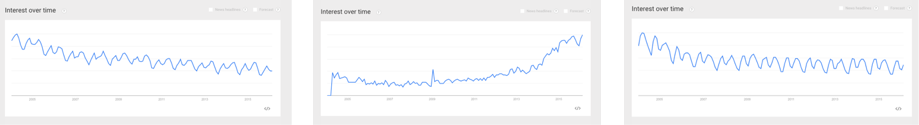
\includegraphics[width=12.76in]{images/googletrends} 

}

\caption{Google trends for different statistical package}\label{fig:googletrend}
\end{figure}

\begin{enumerate}
\def\labelenumi{\arabic{enumi}.}
\setcounter{enumi}{2}
\item
  R is incredibly versatile. You can use R to do everything from calculating simple summary statistics, to performing complex simulations to creating gorgeous plots. If you can imagine an analytical task, you can almost certainly implement it in R.
\item
  Using RStudio, a program to help you write R code, You can easily and seamlessly combine R code, analyses, plots, and written text into elegant documents all in one place using Sweave (R and Latex) or RMarkdown. In fact, I translated this entire book (the text, formatting, plots, code\ldots yes, everything) in RStudio using Sweave. With RStudio and Sweave, instead of trying to manage two or three programs, say Excel, Word and (sigh) SPSS, where you find yourself spending half your time copying, pasting and formatting data, images and test, you can do everything in one place so nothing gets misread, mistyped, or forgotten.
\item
  Analyses conducted in R are transparent, easily shareable, and reproducible. If you ask an SPSS user how they conducted a specific analyses, they will either A) Not remember, B) Try (nervously) to construct an analysis procedure on the spot that makes sense - which may or may not correspond to what they actually did months or years ago, or C) Ask you what you are doing in their house. I used to primarily use SPSS, so I speak from experience on this. If you ask an R user (who uses good programming techniques!) how they conducted an analysis, they should always be able to show you the exact code they used. Of course, this doesn't mean that they used the appropriate analysis or interpreted it correctly, but with all the original code, any problems should be completely transparent!
\end{enumerate}

\hypertarget{rrelationship}{%
\section{Why R is like a relationship\ldots{}}\label{rrelationship}}

Yes, R is very much like a relationship. Like relationships, there are two major truths to R programming:

\begin{figure}

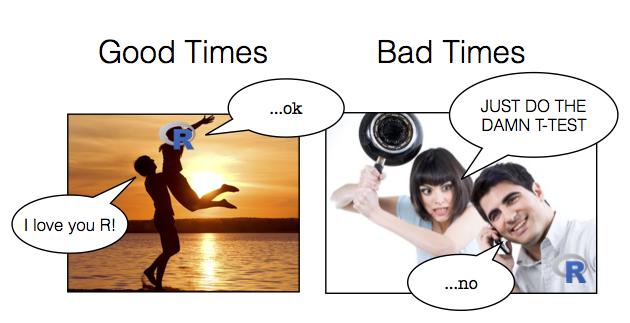
\includegraphics[width=8.75in]{images/rrelationship} \hfill{}

\caption{R will become both your best friend and your worst nightmare. The bad times will make the good times oh so much sweeter.}\label{fig:relationship}
\end{figure}

\begin{enumerate}
\def\labelenumi{\arabic{enumi}.}
\item
  There is nothing more \emph{frustrating} than when your code does \emph{not} work
\item
  There is nothing more \emph{satisfying} than when your code \emph{does} work!
\end{enumerate}

Anything worth doing, from losing weight to getting a degree, takes time. Learning R is no different. Especially if this is your first experience programming, you are going to experience a \emph{lot} of headaches when you get started. You will run into error after error and pound your fists against the table screaming: ``WHY ISN'T MY CODE WORKING?!?!? There must be something wrong with this stupid software!!!'' You will spend hours trying to find a bug in your code, only to find that - frustratingly enough, you had had an extra space or missed a comma somewhere. You'll then wonder why you ever decided to learn R when (::sigh::) SPSS was so ``nice and easy.''

\begin{figure}

{\centering 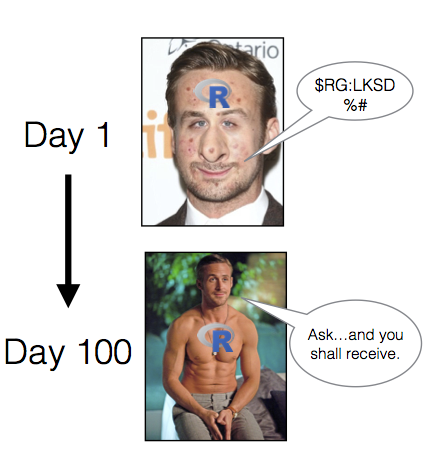
\includegraphics[width=5.99in]{images/gosling} 

}

\caption{When you first meet R, it will look so fugly that you'll wonder if this is all some kind of sick joke. But trust me, once you learn how to talk to it, and clean it up a bit, all your friends will be crazy jealous.}\label{fig:gosling}
\end{figure}

\textbf{Fun Fact!} SPSS stands for ``Shitty Piece of Shitty Shit''. True story.

This is perfectly normal! Don't get discouraged and DON'T GO BACK TO SPSS! That would be quitting on exercise altogether because you had a tough workout.

Trust me, as you gain more programming experience, you'll experience fewer and fewer bugs (though they'll never go away completely). Once you get over the initial barriers, you'll find yourself conducting analyses much, much faster than you ever did before.

\hypertarget{r-resources}{%
\section{R resources}\label{r-resources}}

\hypertarget{r-cheatsheets}{%
\subsection{R Cheatsheets}\label{r-cheatsheets}}

\begin{figure}

{\centering 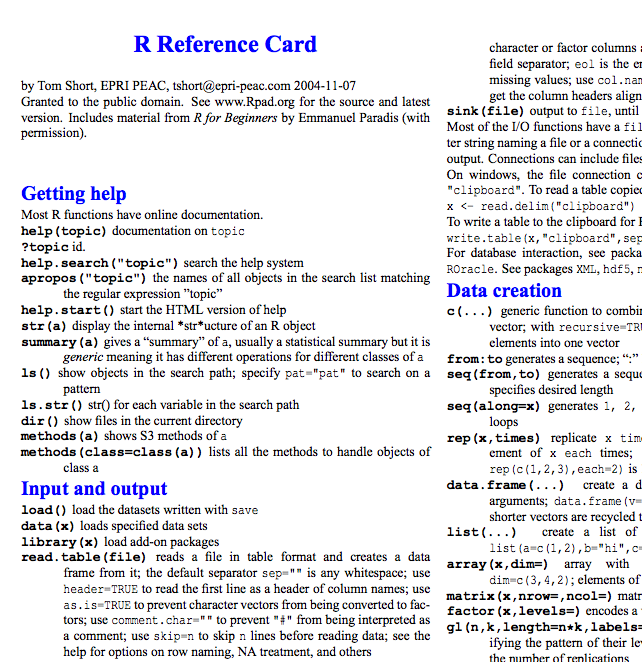
\includegraphics[width=0.75\linewidth]{images/rreferencess} 

}

\caption{The R reference card written by Tom Short is absolutely indispensable!}\label{fig:rreferencecard}
\end{figure}

Over the course of this book, you will be learning \emph{lots} of new functions. Wouldn't it be nice if someone created a Cheatsheet / Dictionary of many common R functions? Yes it would, and thankfully several friendly R programmers have done just that. Below is a table of some of them that I recommend. I highly encourage you to print these out and start highlighting functions as you learn them!

\begin{longtable}[]{@{}lll@{}}
\toprule
\begin{minipage}[b]{0.37\columnwidth}\raggedright
CheatSheet\strut
\end{minipage} & \begin{minipage}[b]{0.18\columnwidth}\raggedright
Author\strut
\end{minipage} & \begin{minipage}[b]{0.36\columnwidth}\raggedright
Link\strut
\end{minipage}\tabularnewline
\midrule
\endhead
\begin{minipage}[t]{0.37\columnwidth}\raggedright
R Basics\strut
\end{minipage} & \begin{minipage}[t]{0.18\columnwidth}\raggedright
Tom Short\strut
\end{minipage} & \begin{minipage}[t]{0.36\columnwidth}\raggedright
\url{https://cran.r-project.org/doc/contrib/Short-refcard.pdf}\strut
\end{minipage}\tabularnewline
\begin{minipage}[t]{0.37\columnwidth}\raggedright
Advanced R\strut
\end{minipage} & \begin{minipage}[t]{0.18\columnwidth}\raggedright
Arianne Colton and Sean Chen\strut
\end{minipage} & \begin{minipage}[t]{0.36\columnwidth}\raggedright
\href{https://www.rstudio.com/wp-content/uploads/2016/02/advancedR.pdf}{hhttps://www.rstudio.com/wp-content/uploads/2016/02/advancedR.pdf}\strut
\end{minipage}\tabularnewline
\begin{minipage}[t]{0.37\columnwidth}\raggedright
Base R\strut
\end{minipage} & \begin{minipage}[t]{0.18\columnwidth}\raggedright
\href{http://mhairihmcneill.com/}{Mhairi McNeill}\strut
\end{minipage} & \begin{minipage}[t]{0.36\columnwidth}\raggedright
\url{http://github.com/rstudio/cheatsheets/raw/master/base-r.pdf}\strut
\end{minipage}\tabularnewline
\begin{minipage}[t]{0.37\columnwidth}\raggedright
Strings\strut
\end{minipage} & \begin{minipage}[t]{0.18\columnwidth}\raggedright
\href{https://www.rstudio.com}{RStudio}\strut
\end{minipage} & \begin{minipage}[t]{0.36\columnwidth}\raggedright
\url{https://github.com/rstudio/cheatsheets/raw/master/strings.pdf}\strut
\end{minipage}\tabularnewline
\begin{minipage}[t]{0.37\columnwidth}\raggedright
Data import\strut
\end{minipage} & \begin{minipage}[t]{0.18\columnwidth}\raggedright
\href{https://www.rstudio.com}{RStudio}\strut
\end{minipage} & \begin{minipage}[t]{0.36\columnwidth}\raggedright
\url{https://github.com/rstudio/cheatsheets/raw/master/data-import.pdf}\strut
\end{minipage}\tabularnewline
\begin{minipage}[t]{0.37\columnwidth}\raggedright
Data transformation\strut
\end{minipage} & \begin{minipage}[t]{0.18\columnwidth}\raggedright
\href{https://www.rstudio.com}{RStudio}\strut
\end{minipage} & \begin{minipage}[t]{0.36\columnwidth}\raggedright
\url{https://github.com/rstudio/cheatsheets/raw/master/data-import.pdf}\strut
\end{minipage}\tabularnewline
\begin{minipage}[t]{0.37\columnwidth}\raggedright
RStudio application\strut
\end{minipage} & \begin{minipage}[t]{0.18\columnwidth}\raggedright
\href{https://www.rstudio.com}{RStudio}\strut
\end{minipage} & \begin{minipage}[t]{0.36\columnwidth}\raggedright
\url{https://github.com/rstudio/cheatsheets/raw/master/rstudio-ide.pdf}\strut
\end{minipage}\tabularnewline
\begin{minipage}[t]{0.37\columnwidth}\raggedright
Plotting with ggplot2\strut
\end{minipage} & \begin{minipage}[t]{0.18\columnwidth}\raggedright
\href{https://www.rstudio.com}{RStudio}\strut
\end{minipage} & \begin{minipage}[t]{0.36\columnwidth}\raggedright
\url{https://github.com/rstudio/cheatsheets/raw/master/data-visualization-2.1.pdf}\strut
\end{minipage}\tabularnewline
\begin{minipage}[t]{0.37\columnwidth}\raggedright
RMarkdown\strut
\end{minipage} & \begin{minipage}[t]{0.18\columnwidth}\raggedright
\href{https://www.rstudio.com}{RStudio}\strut
\end{minipage} & \begin{minipage}[t]{0.36\columnwidth}\raggedright
\url{https://www.rstudio.com/wp-content/uploads/2015/03/rmarkdown-reference.pdf}\strut
\end{minipage}\tabularnewline
\bottomrule
\end{longtable}

\hypertarget{getting-r-help-and-inspiration-online}{%
\subsection{Getting R help and inspiration online}\label{getting-r-help-and-inspiration-online}}

Here are some great resources for R help and inspiration:

\begin{longtable}[]{@{}ll@{}}
\toprule
\begin{minipage}[b]{0.42\columnwidth}\raggedright
Site\strut
\end{minipage} & \begin{minipage}[b]{0.52\columnwidth}\raggedright
Description\strut
\end{minipage}\tabularnewline
\midrule
\endhead
\begin{minipage}[t]{0.42\columnwidth}\raggedright
\href{http://www.google.com}{www.google.com}\strut
\end{minipage} & \begin{minipage}[t]{0.52\columnwidth}\raggedright
Seriously, Google is any programmer's best friend. More likely than not you will be directed to \url{www.stackoverflow.com} or \url{www.stackexchange.com}\strut
\end{minipage}\tabularnewline
\begin{minipage}[t]{0.42\columnwidth}\raggedright
\href{http://www.r-bloggers.com}{www.r-bloggers.com}\strut
\end{minipage} & \begin{minipage}[t]{0.52\columnwidth}\raggedright
R bloggers is my go-to place to discover the latest and greatest with R.\strut
\end{minipage}\tabularnewline
\begin{minipage}[t]{0.42\columnwidth}\raggedright
\href{http://blog.revolutionanalytics.com}{blog.revolutionanalytics.com}\strut
\end{minipage} & \begin{minipage}[t]{0.52\columnwidth}\raggedright
Revolution analytics always has great R related material.\strut
\end{minipage}\tabularnewline
\bottomrule
\end{longtable}

\hypertarget{other-r-books}{%
\subsection{Other R books}\label{other-r-books}}

There are many, many excellent (non-pirate) books on R, some of which are available online for free. Here are some that I highly recommend:

\begin{longtable}[]{@{}ll@{}}
\toprule
\begin{minipage}[b]{0.42\columnwidth}\raggedright
Book\strut
\end{minipage} & \begin{minipage}[b]{0.52\columnwidth}\raggedright
Description\strut
\end{minipage}\tabularnewline
\midrule
\endhead
\begin{minipage}[t]{0.42\columnwidth}\raggedright
\href{http://r4ds.had.co.nz/}{R for Data Science by Garrett Grolemund and Hadley Wickham}\strut
\end{minipage} & \begin{minipage}[t]{0.52\columnwidth}\raggedright
The best book to learn the latest tools for elegantly doing data science.\strut
\end{minipage}\tabularnewline
\begin{minipage}[t]{0.42\columnwidth}\raggedright
\href{http://www.cookbook-r.com/Graphs/}{R Graphics Cookbook by Winston Chang}\strut
\end{minipage} & \begin{minipage}[t]{0.52\columnwidth}\raggedright
is indispensible for creating graphics.\strut
\end{minipage}\tabularnewline
\begin{minipage}[t]{0.42\columnwidth}\raggedright
\href{https://rc2e.com/index.html}{R Cookbook by James (JD) Long and Paul Teetor}\strut
\end{minipage} & \begin{minipage}[t]{0.52\columnwidth}\raggedright
is a useful bag of tips and tricks to get started with R .\strut
\end{minipage}\tabularnewline
\begin{minipage}[t]{0.42\columnwidth}\raggedright
\href{https://www.amazon.com/Discovering-Statistics-Using-Andy-Field/dp/1446200469/ref=sr_1_2?ie=UTF8\&qid=1487759316\&sr=8-2\&keywords=statistics+with+r}{Discovering Statistics with R by Field, Miles and Field}\strut
\end{minipage} & \begin{minipage}[t]{0.52\columnwidth}\raggedright
A classic text focusing on the theory and practice of statistical analysis with R\strut
\end{minipage}\tabularnewline
\bottomrule
\end{longtable}

\hypertarget{started}{%
\chapter{Getting Started}\label{started}}

\hypertarget{installing-base-r-and-rstudio}{%
\section{Installing Base-R and RStudio}\label{installing-base-r-and-rstudio}}

To use R, we'll need to download two software packages: \textbf{Base-R}, and \textbf{RStudio}. Base-R is the basic software which contains the R programming language. RStudio is software that makes R programming easier. In everyday parlance, R is the engine and RStudio is the car's frame. Just like you can transfer an engine to different car frames, you can use R using other platforms. But I will use RStudio. Of course, they are totally free and open source.

\hypertarget{check-for-version-updates}{%
\subsection{Check for version updates}\label{check-for-version-updates}}

R and RStudio have been around for several years -- however, they are \emph{constantly} being updated with new features and bug-fixes. At the time that I am writing this sentence (10:00, Friday, 6 Sep 2019), the latest version of Base-R is 3.6.1 which was released on 5 Jul 2019, and the latest version of RStudio is 1.2.1335 released on 8 Apr 2019.

\begin{figure}

{\centering \includegraphics[width=0.4\linewidth]{images/rlogo} 

}

\caption{R logo}\label{fig:rlogo}
\end{figure}

To install Base-R, click on one of the following links and follow the instructions.

\begin{longtable}[]{@{}ll@{}}
\toprule
Operating System & Link\tabularnewline
\midrule
\endhead
Windows & \url{http://cran.r-project.org/bin/windows/base/}\tabularnewline
Mac & \url{http://cran.r-project.org/bin/macosx/}\tabularnewline
\bottomrule
\end{longtable}

Once you've installed base-R on your computer, try opening it. When you do you should see a screen like the one in Figure \ref{fig:rscreenshot} (this is the Windows version). As you can see, base R is very much bare-bones software. It's kind of the equivalent of a simple text editor that comes with your computer.

\begin{figure}

{\centering 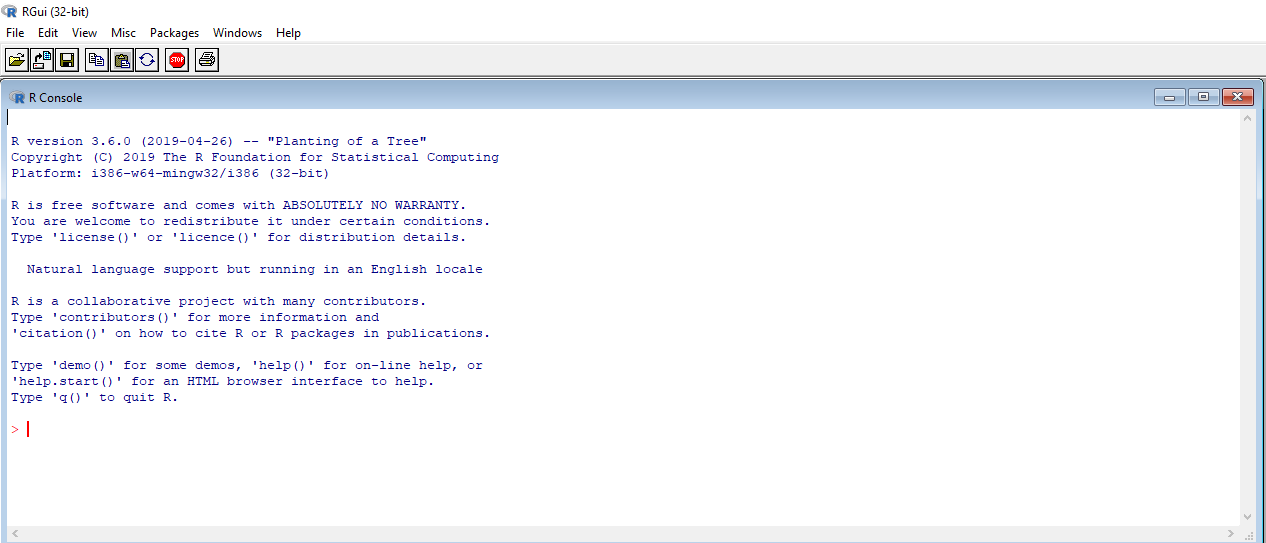
\includegraphics[width=0.75\linewidth]{images/RScreenshot} 

}

\caption{Here is how the base R application looks. While you can use the base R application alone, most people I know use RStudio -- software that helps you to write and use R code more efficiently!}\label{fig:rscreenshot}
\end{figure}

\begin{figure}

{\centering 
\includegraphics[width=0.4\linewidth]{images/RStudio} 

}

\caption{RStudio logo}\label{fig:rstudiologo}
\end{figure}

While you can do pretty much everything you want within base-R, you'll find that most people these days do their R programming in an application called RStudio. RStudio is a graphical user interface (GUI)-like interface for R that makes programming in R a bit easier. In fact, once you've installed RStudio, you'll likely never need to open the base R application again. To download and install RStudio (around 40mb), go to\url{http://www.rstudio.com/products/rstudio/download/}\textbar{} and follow the instructions.

Let's go ahead and boot up RStudio and see how she looks!

\hypertarget{the-four-rstudio-windows}{%
\section{The four RStudio Windows}\label{the-four-rstudio-windows}}

When you open RStudio, you'll see the following four windows (also called panes) shown in in Figure \ref{fig:rstudiowindows}. However, your windows might be in a different order that those in Figure \ref{fig:rstudiowindows}. If you'd like, you can change the order of the windows under RStudio preferences. You can also change their shape by either clicking the minimize or maximize buttons on the top right of each panel, or by clicking and dragging the middle of the borders of the windows.

\begin{figure}

{\centering 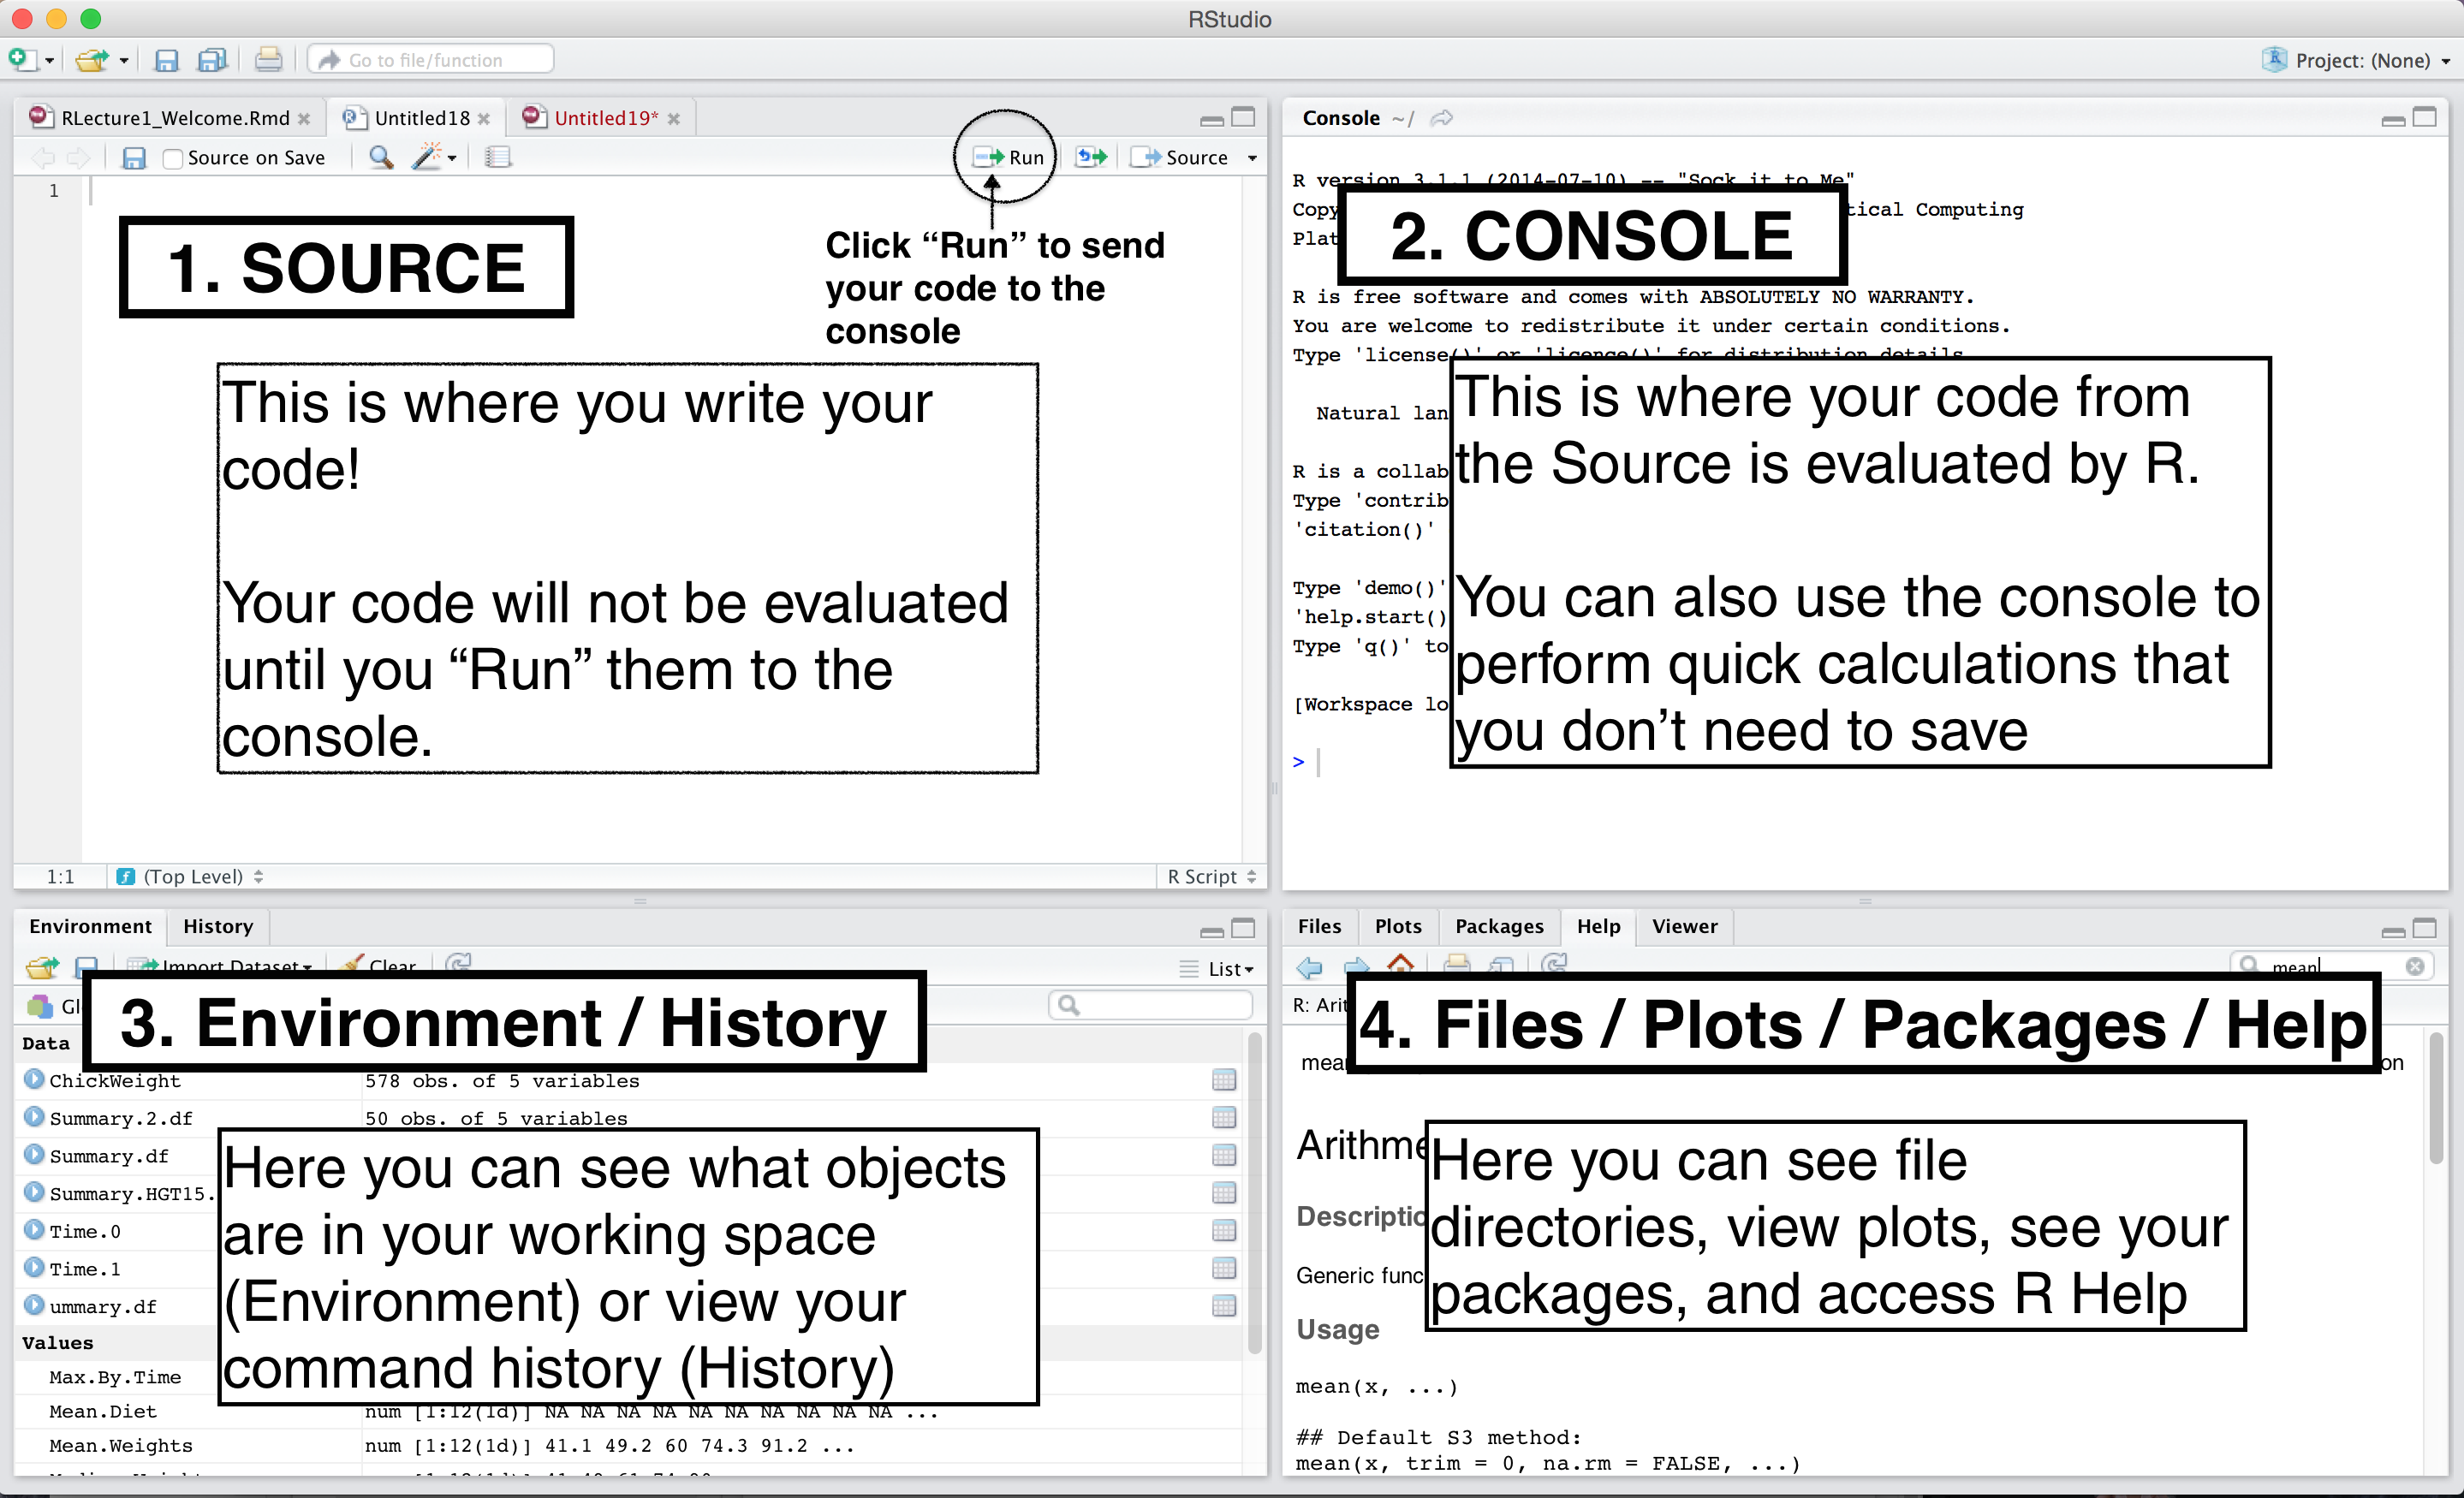
\includegraphics[width=1\linewidth]{images/RStudio_Screenshot_Labels} 

}

\caption{The four panes of RStudio.}\label{fig:rstudiowindows}
\end{figure}

Now, let's see what each window does in detail.

\hypertarget{source---your-notepad-for-code}{%
\subsection{Source - Your notepad for code}\label{source---your-notepad-for-code}}

\begin{figure}

{\centering 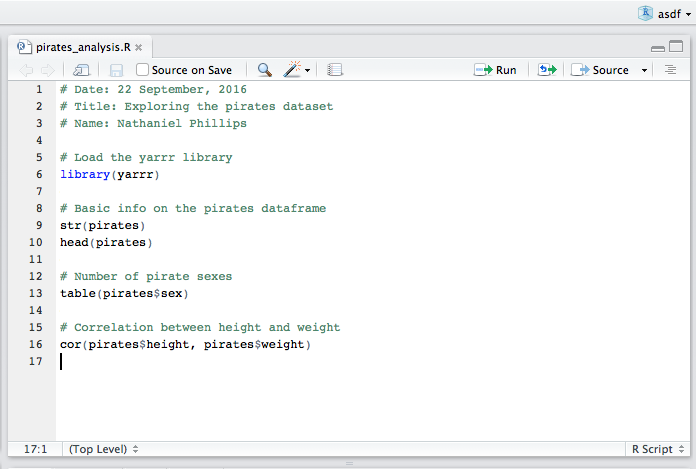
\includegraphics[width=1\linewidth]{images/piratesanalysisss} 

}

\caption{The Source contains all of your individual R scripts. The code won't be evaluated until you send it to the Console.}\label{fig:sourcewindow}
\end{figure}

The source pane is where you create and edit ``R Scripts'' - your collections of code. Don't worry, R scripts are just text files with the ``.R'' extension. When you open RStudio, it will automatically start a new Untitled script. Before you start typing in an untitled R script, you should always save the file under a new file name (like, ``StatsAnal.R''). That way, if something on your computer crashes while you're working, R will have your code waiting for you when you re-open RStudio.

You'll notice that when you're typing code in a script in the Source panel, R won't actually evaluate the code as you type. To have R actually evaluate your code, you need to first `send' the code to the Console (we'll talk about this in the next section).

There are many ways to send your code from the Source to the console. The slowest way is to copy and paste. A faster way is to highlight the code you wish to evaluate and clicking on the ``Run'' button on the top right of the Source. Alternatively, you can use the hot-key ``Command + Return'' on Mac, or ``Control + Enter'' on PC to send all highlighted code to the console.

\hypertarget{console-rs-heart}{%
\subsection{Console: R's Heart}\label{console-rs-heart}}

\begin{figure}
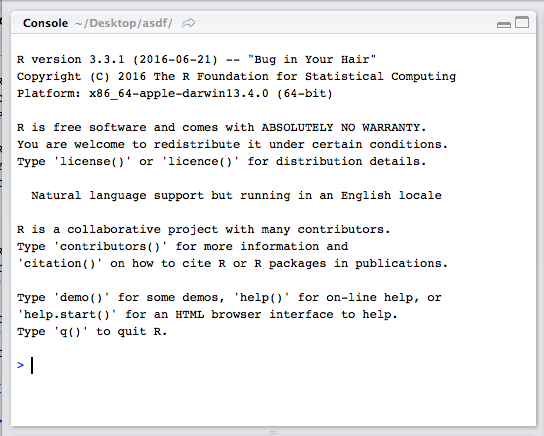
\includegraphics[width=0.75\linewidth]{images/consoless} \caption{The console the calculation heart of R. All of your code will (eventually) go through here.}\label{fig:consolewindow}
\end{figure}

The console is the heart of R. Here is where R actually evaluates code. At the beginning of the console you'll see the character \texttt{>}. This is a prompt that tells you that R is ready for new code. You can type code directly into the console after the \texttt{>} prompt and get an immediate response. For example, if you type 1+1 into the console and press enter, you'll see that R immediately gives an output of 2.

\begin{Shaded}
\begin{Highlighting}[]
\DecValTok{1}\OperatorTok{+}\DecValTok{1}
\end{Highlighting}
\end{Shaded}

\begin{verbatim}
## [1] 2
\end{verbatim}

Try calculating 1+1 by typing the code directly into the console - then press Enter. You should see the result {[}1{]} 2. Don't worry about the {[}1{]} for now, we'll get to that later. For now, we're happy if we just see the 2. Then, type the same code into the Source, and then send the code to the Console by highlighting the code and clicking the ``Run" button on the top right hand corner of the Source window. Alternatively, you can use the hot-key ``Command + Return'' on Mac or ``Control + Enter'' on Windows.

\textbf{Tip}: Try to write most of your code in a document in the Source. Only type directly into the Console to de-bug or do quick analyses.

So as you can see, you can execute code either by running it from the Source or by typing it directly into the Console. However, 99\% most of the time, you should be using the Source rather than the Console. The reason for this is straightforward: If you type code into the console, it won't be saved (though you can look back on your command History). And if you make a mistake in typing code into the console, you'd have to re-type everything all over again. Instead, it's better to write all your code in the Source. When you are ready to execute some code, you can then send ``Run'' it to the console.

\hypertarget{environment-history}{%
\subsection{Environment / History}\label{environment-history}}

\begin{figure}
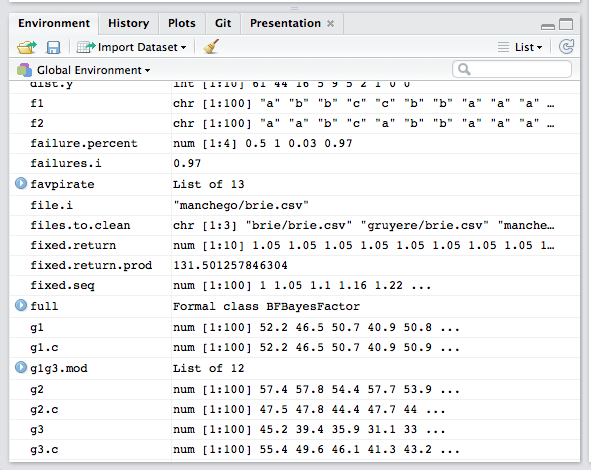
\includegraphics[width=0.75\linewidth]{images/environmentss} \caption{The environment panel shows you all the objects you have defined in your current workspace. You'll learn more about workspaces in Chapter 7.}\label{fig:environwindow}
\end{figure}

The Environment tab of this panel shows you the names of all the data objects (like vectors, matrices, and dataframes) that you've defined in your current R session. You can also see information like the number of observations and rows in data objects. The tab also has a few clickable actions like ``Import Dataset" which will open a graphical user interface (GUI) for important data into R. However, I almost never look at this menu.

The History tab of this panel simply shows you a history of all the code you've previously evaluated in the Console. To be honest, I never look at this. In fact, I didn't realize it was even there until I started writing this tutorial.

As you get more comfortable with R, you might find the Environment / History panel useful. But for now you can just ignore it. If you want to declutter your screen, you can even just minimize the window by clicking the minimize button on the top right of the panel.

\hypertarget{files-plots-packages-help}{%
\subsection{Files / Plots / Packages / Help}\label{files-plots-packages-help}}

The Files / Plots / Packages / Help panel shows you lots of helpful information. Let's go through each tab in detail:

\begin{enumerate}
\def\labelenumi{\arabic{enumi}.}
\item
  Files - The files panel gives you access to the file directory on your hard drive. One nice feature of the ``Files'' panel is that you can use it to set your working directory - once you navigate to a folder you want to read and save files to, click ``More'' and then ``Set As Working Directory.'' We'll talk about working directories in more detail soon.
\item
  Plots - The Plots panel (no big surprise), shows all your plots. There are buttons for opening the plot in a separate window and exporting the plot as a pdf or jpeg (though you can also do this with code using the \texttt{pdf()} or \texttt{jpeg()} functions.)
\end{enumerate}

Let's see how plots are displayed in the Plots panel. Run the code on the right to display a histogram of the weights of chickens stored in the \texttt{ChickWeight} dataset. When you do, you should see a plot similar to the one in Figure \ref{fig:plotpanel} show up in the Plots panel.

\begin{Shaded}
\begin{Highlighting}[]
\KeywordTok{hist}\NormalTok{(}\DataTypeTok{x =}\NormalTok{ ChickWeight}\OperatorTok{$}\NormalTok{weight,}
     \DataTypeTok{main =} \StringTok{"Chicken Weights"}\NormalTok{,}
     \DataTypeTok{xlab =} \StringTok{"Weight"}\NormalTok{,}
     \DataTypeTok{col =} \StringTok{"skyblue"}\NormalTok{,}
     \DataTypeTok{border =} \StringTok{"white"}\NormalTok{)}
\end{Highlighting}
\end{Shaded}

\begin{figure}
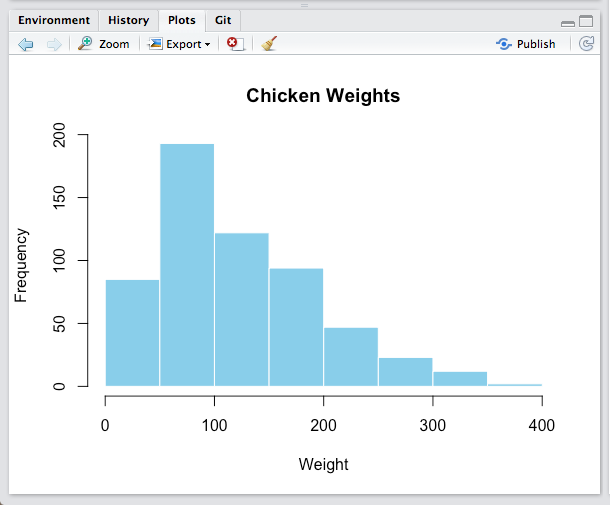
\includegraphics[width=0.75\linewidth]{images/plotpanelss} \caption{The plot panel contains all of your plots, like this histogram of the distribution of chicken weights.}\label{fig:plotpanel}
\end{figure}

\begin{enumerate}
\def\labelenumi{\arabic{enumi}.}
\setcounter{enumi}{2}
\item
  Packages - Shows a list of all the R packages installed on your harddrive and indicates whether or not they are currently loaded. Packages that are loaded in the current session are checked while those that are installed but not yet loaded are unchecked. We'll discuss packages in more detail in the next section.
\item
  Help - Help menu for R functions. You can either type the name of a function in the search window, or use the code \texttt{?function.name} to search for a function with the name \texttt{function.name}
\end{enumerate}

\begin{Shaded}
\begin{Highlighting}[]
\NormalTok{?hist   }\CommentTok{# How does the histogram function work?}
\NormalTok{?t.test }\CommentTok{# What about a t-test?}
\end{Highlighting}
\end{Shaded}

\hypertarget{reading-and-writing-code}{%
\section{Reading and writing Code}\label{reading-and-writing-code}}

\hypertarget{code-chunks}{%
\subsection{Code Chunks}\label{code-chunks}}

In this book, R code is (almost) always presented in a separate gray box like this one:

\begin{Shaded}
\begin{Highlighting}[]
\CommentTok{# A code chunk}

\CommentTok{# Define a vector a as the integers from 1 to 5}
\NormalTok{a <-}\StringTok{ }\DecValTok{1}\OperatorTok{:}\DecValTok{5}

\CommentTok{# Print a}
\NormalTok{a}
\end{Highlighting}
\end{Shaded}

\begin{verbatim}
## [1] 1 2 3 4 5
\end{verbatim}

\begin{Shaded}
\begin{Highlighting}[]
\CommentTok{# What is the mean of a?}
\KeywordTok{mean}\NormalTok{(a)}
\end{Highlighting}
\end{Shaded}

\begin{verbatim}
## [1] 3
\end{verbatim}

This is called a \emph{code chunk}. You should always be able to copy and paste code chunks directly into R. If you copy a chunk and it does not work for you, it is most likely because the code refers to a package, function, or object that I defined in a previous chunk. If so, read back and look for a previous chunk that contains the missing definition.

\hypertarget{comments-with}{%
\subsection{Comments with \#}\label{comments-with}}

Lines that begin with \# are comments. If you evaluate any code that starts with \#, R will just ignore that line. In this book, comments will be either be literal comments that I write directly to explain code, or they will be \emph{output} generated automatically from R. For example, in the code chunk below, you see lines starting with \#\#. These are the output from the previous line(s) of code. When you run the code yourself, you should see the same output in your \emph{console}.

\begin{Shaded}
\begin{Highlighting}[]
\CommentTok{# This is a comment I wrote}

\DecValTok{1} \OperatorTok{+}\StringTok{ }\DecValTok{2}
\end{Highlighting}
\end{Shaded}

\begin{verbatim}
## [1] 3
\end{verbatim}

\begin{Shaded}
\begin{Highlighting}[]
\CommentTok{# The line above (## [1] 3) is the output from the previous code that has been 'commented out'}
\end{Highlighting}
\end{Shaded}

\hypertarget{element-numbers-in-output-1}{%
\subsection{Element numbers in output {[}1{]}}\label{element-numbers-in-output-1}}

The output you see will often start with one or more number(s) in brackets such as {[}1{]}. This is just a visual way of telling you where the numbers occur in the output. For example, in the code below, I will print a long vector containing the multiples of 2 from 0 to 100:

\begin{Shaded}
\begin{Highlighting}[]
\KeywordTok{seq}\NormalTok{(}\DataTypeTok{from =} \DecValTok{0}\NormalTok{, }\DataTypeTok{to =} \DecValTok{100}\NormalTok{, }\DataTypeTok{by =} \DecValTok{2}\NormalTok{)}
\end{Highlighting}
\end{Shaded}

\begin{verbatim}
##  [1]   0   2   4   6   8  10  12  14  16  18  20  22  24  26  28  30  32  34  36
## [20]  38  40  42  44  46  48  50  52  54  56  58  60  62  64  66  68  70  72  74
## [39]  76  78  80  82  84  86  88  90  92  94  96  98 100
\end{verbatim}

As you can see, the first line of the output starts with \#\# {[}1{]}, and the next two lines start with {[}18{]} and {[}35{]}. This is just telling you that 0 is the {[}1{]}st element, 34 is the {[}18{]}th element, and 68 is the {[}35{]}th element. Sometimes this information will be helpful, but most of the time you can just ignore it.

\hypertarget{debugging}{%
\section{Debugging}\label{debugging}}

When you are programming, you will always, and I do mean always, make errors (also called bugs) in your code. You might misspell a function, include an extra comma, or some days\ldots R just won't want to work with you (again, see section \protect\hyperlink{rrelationship}{Why R is like a Relationship}).

Debugging will always be a challenge. However, over time you'll learn which bugs are the most common and get faster and faster at finding and correcting them.

Here are the most common bugs you'll run into as you start your R journey.

\hypertarget{r-is-not-ready}{%
\subsection{R is not ready (\textgreater)}\label{r-is-not-ready}}

Another very common problem occurs when R does not seem to be responding to your code. That is, you might run some code like \texttt{mean(x)} expecting some output, but instead, nothing happens. This can be very frustrating because, rather than getting an error, just nothing happens at all. The most common reason for this is because R isn't \emph{ready} for new code, instead, it is \emph{waiting} for you to finish code you started earlier, but never properly finished.

Think about it this way, R can be in one of two states: it is either \textbf{Ready} (\textgreater) for new code, or it is \textbf{Waiting} (+) for you to finish old code. To see which state R is in, all you have to do is look at the symbol on the console. The \texttt{\textgreater{}} symbol means that R is Ready for new code -- this is usually what you want to see. The \texttt{+} symbol means that R is Waiting for you to (properly) finish code you started before. If you see the \texttt{+} symbol, then no matter how much new code you write, R won't actually evaluate it until you finish the code you started before.

Thankfully there is an easy solution to this problem (See Figure \ref{fig:rstate}): Just hit the escape key on your keyboard. This will cancel R's waiting state and make it Ready!

\begin{figure}

{\centering 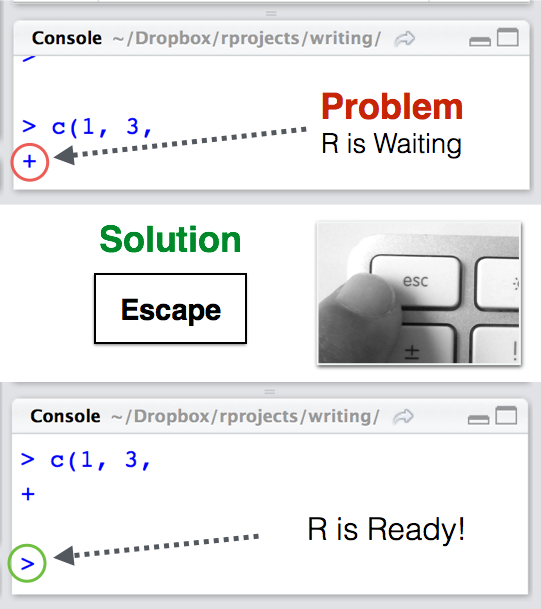
\includegraphics[width=0.5\linewidth]{images/escapesolution} 

}

\caption{To turn R from a Waiting (+) state to a Ready (>) state, just hit Escape.}\label{fig:rstate}
\end{figure}

\hypertarget{misspelled-object-or-function}{%
\subsection{Misspelled object or function}\label{misspelled-object-or-function}}

If you spell an object or function incorrectly, you'll receive an error like \texttt{Error:\ could\ not\ find\ function} or \texttt{Error:\ object\ \textquotesingle{}x\textquotesingle{}\ not\ found}.

In the code below, I'll try to take the mean of a vector \texttt{data}, but I will misspell the function \texttt{mean()}

\begin{Shaded}
\begin{Highlighting}[]
\NormalTok{data <-}\StringTok{ }\KeywordTok{c}\NormalTok{(}\DecValTok{1}\NormalTok{, }\DecValTok{4}\NormalTok{, }\DecValTok{3}\NormalTok{, }\DecValTok{2}\NormalTok{, }\DecValTok{1}\NormalTok{)}

\CommentTok{# Misspelled function: should be mean(x), not meeen(x)}
\KeywordTok{meeen}\NormalTok{(data)}
\end{Highlighting}
\end{Shaded}

\begin{error}

Error: could not find function ``meeen''

\end{error}

Now, I'll misspell the object \texttt{data} as \texttt{dta}:

\begin{Shaded}
\begin{Highlighting}[]
\CommentTok{# Misspelled object: should be data, not dta}
\KeywordTok{mean}\NormalTok{(dta)}
\end{Highlighting}
\end{Shaded}

\begin{error}

Error: object `dta' not found

\end{error}

R is case-sensitive, so if you don't use the correct capitalization you'll receive an error. In the code below, I'll use \texttt{Mean()} instead of the correct version \texttt{mean()}

\begin{Shaded}
\begin{Highlighting}[]
\CommentTok{# Capitalization is wrong: should be mean(), not Mean()}
\KeywordTok{Mean}\NormalTok{(data)}
\end{Highlighting}
\end{Shaded}

\begin{error}

Error: could not find function ``Mean''

\end{error}

Here is the correct version where both the object \texttt{data} and function \texttt{mean()} are correctly spelled:

\begin{Shaded}
\begin{Highlighting}[]
\CommentTok{# Correct: both the object and function are correctly spelled}
\KeywordTok{mean}\NormalTok{(data)}
\end{Highlighting}
\end{Shaded}

\begin{verbatim}
## [1] 2.2
\end{verbatim}

\hypertarget{punctuation-problems}{%
\subsection{Punctuation problems}\label{punctuation-problems}}

Another common error is having bad coding ``punctuation''. By that, I mean having an extra space, missing a comma, or using a comma (,) instead of a period (.). In the code below, I'll try to create a vector using periods instead of commas:

\begin{Shaded}
\begin{Highlighting}[]
\CommentTok{# Wrong: Using periods (.) instead of commas (,)}
\KeywordTok{mean}\NormalTok{(}\KeywordTok{c}\NormalTok{(}\FloatTok{1.} \FloatTok{4.} \DecValTok{2}\NormalTok{))}
\end{Highlighting}
\end{Shaded}

\begin{error}

Error: unexpected numeric constant in ``mean(c(1. 4.''

\end{error}

Because I used periods instead of commas, I get the above error. Here is the correct version

\begin{Shaded}
\begin{Highlighting}[]
\CommentTok{# Correct}
\KeywordTok{mean}\NormalTok{(}\KeywordTok{c}\NormalTok{(}\DecValTok{1}\NormalTok{, }\DecValTok{4}\NormalTok{, }\DecValTok{2}\NormalTok{))}
\end{Highlighting}
\end{Shaded}

\begin{verbatim}
## [1] 2.333333
\end{verbatim}

If you include an extra space in the middle of the name of an object or function, you'll receive an error. In the code below, I'll accidentally write \texttt{Chick\ Weight} instead of \texttt{ChickWeight}:

\begin{Shaded}
\begin{Highlighting}[]
\CommentTok{# Wrong: Extra space in the ChickWeight object name}
\KeywordTok{head}\NormalTok{(Chick Weight)}
\end{Highlighting}
\end{Shaded}

\begin{error}

Error: unexpected symbol in ``head(Chick Weight''

\end{error}

Because I had an extra space in the object name, I get the above error. Here is the correction:

\begin{Shaded}
\begin{Highlighting}[]
\CommentTok{# Correct:}
\KeywordTok{head}\NormalTok{(ChickWeight)}
\end{Highlighting}
\end{Shaded}

\hypertarget{learning-check}{%
\section*{Learning check}\label{learning-check}}
\addcontentsline{toc}{section}{Learning check}

\begin{enumerate}
\def\labelenumi{\arabic{enumi}.}
\item
  Download R software and RStudio software
\item
  Open up RStudio software and type the following code below into the \textbf{console}. What does it give you?
\end{enumerate}

\begin{Shaded}
\begin{Highlighting}[]
\DecValTok{1}\OperatorTok{+}\DecValTok{10}
\end{Highlighting}
\end{Shaded}

\begin{enumerate}
\def\labelenumi{\arabic{enumi}.}
\setcounter{enumi}{2}
\tightlist
\item
  Look at the code below. What will R return after the third line? Make a prediction, then test the code yourself.
\end{enumerate}

\begin{Shaded}
\begin{Highlighting}[]
\NormalTok{a <-}\StringTok{ }\DecValTok{10}
\NormalTok{a }\OperatorTok{+}\StringTok{ }\DecValTok{10}
\NormalTok{a}
\end{Highlighting}
\end{Shaded}

\hypertarget{basics}{%
\chapter{The Basics}\label{basics}}

\hypertarget{download-and-load-libraries}{%
\section{Download and load libraries}\label{download-and-load-libraries}}

Libraries are like your iphone apps. The iphone comes with some basic functionality, e.g.~weather. If you wanted more, you have to download. Subsequent chapters are going to start with this code chunk. This is only needed if you are running one chapter independent from others. Notice how I am using the package called \texttt{pacman}. This is a package manager, which loads any package you typed into it, and if it is not available, download it automatically from CRAN and load it.

\begin{Shaded}
\begin{Highlighting}[]
\ControlFlowTok{if}\NormalTok{ (}\OperatorTok{!}\KeywordTok{require}\NormalTok{(}\StringTok{"pacman"}\NormalTok{)) }\KeywordTok{install.packages}\NormalTok{(}\StringTok{"pacman"}\NormalTok{)}
\NormalTok{pacman}\OperatorTok{::}\KeywordTok{p_load}\NormalTok{(tidyverse, }\CommentTok{# All purpose wrangling for dataframes}
\NormalTok{               readr, }\CommentTok{# importing and writing data}
\NormalTok{               readxl,}\CommentTok{# read and write excel documents}
\NormalTok{               purrr, }\CommentTok{# for piping %>%}
\NormalTok{               corrplot, }\CommentTok{# for correlation}
\NormalTok{               knitr,}
\NormalTok{               yarrr)}
\end{Highlighting}
\end{Shaded}

If you're like most people, you think of R as a statistics program. However, while R is definitely the coolest, most badass, pirate-y way to conduct statistics -- it's not really a program. Rather, it's a programming \emph{language} that was written by and for statisticians.

In this chapter, we'll go over the basics of the R language and the RStudio programming environment.

\hypertarget{the-command-line-console}{%
\section{The command-line (Console)}\label{the-command-line-console}}

\begin{figure}

{\centering 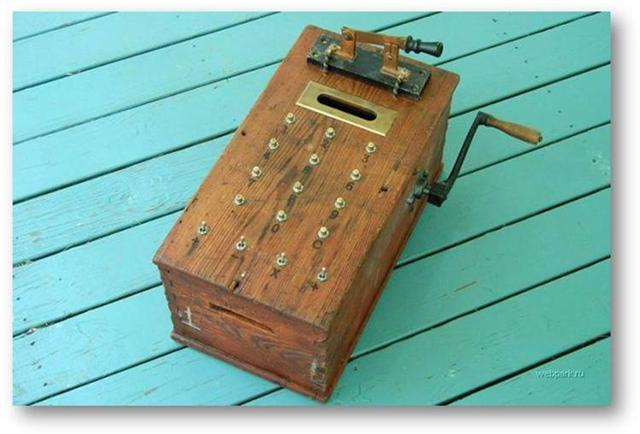
\includegraphics[width=0.5\linewidth]{images/woodcalc} 

}

\caption{Yep. R is really just a fancy calculator. This R programming device was found on a shipwreck on the Bodensee in Germany. I stole it from a museum and made a pretty sweet plot with it. But I don't want to show it to you.}\label{fig:unnamed-chunk-2}
\end{figure}

R code, on its own, is just text. You can write R code in a new script within R or RStudio, or in any text editor. Hell, you can write R code on Twitter if you want. However, just writing the code won't do the whole job -- in order for your code to be executed (aka, interpreted) you need to send it to R's \emph{command-line interpreter}. In RStudio, the command-line interpreter is called the Console.

\begin{figure}

{\centering 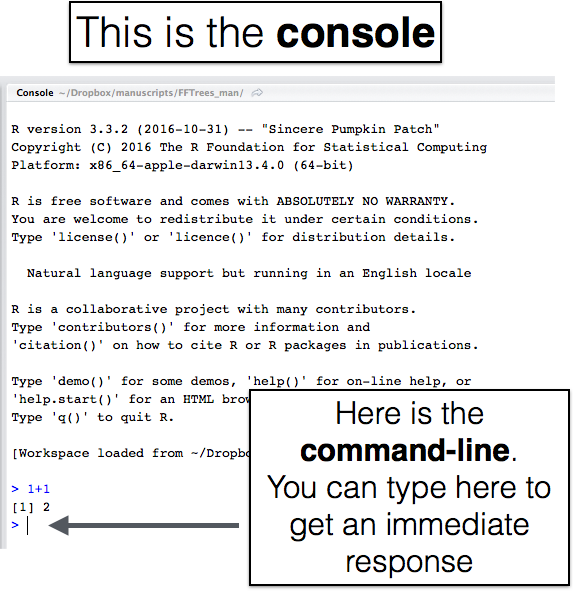
\includegraphics[width=0.75\linewidth]{images/commandline} 

}

\caption{You can always type code directly into the command line to get an immediate response.}\label{fig:unnamed-chunk-3}
\end{figure}

In R, the command-line interpreter starts with the \texttt{\textgreater{}} symbol. This is called the \textbf{prompt}. Why is it called the prompt? Well, it's ``prompting'' you to feed it with some R code. The fastest way to have R evaluate code is to type your R code directly into the command-line interpreter. For example, if you type \texttt{1+1} into the interpreter and hit enter you'll see the following

\begin{Shaded}
\begin{Highlighting}[]
\DecValTok{1}\OperatorTok{+}\DecValTok{1}
\end{Highlighting}
\end{Shaded}

\begin{verbatim}
## [1] 2
\end{verbatim}

As you can see, R returned the (thankfully correct) value of 2. You'll notice that the console also returns the text {[}1{]}. This is just telling you you the index of the value next to it. Don't worry about this for now, it will make more sense later. As you can see, R can, thankfully, do basic calculations. In fact, at its heart, R is technically just a fancy calculator. But that's like saying Michael Jordan is \emph{just} a fancy ball bouncer or Donald Trump is \emph{just} an orange with a dead fox on his head. It (and they), are much more than that.

\hypertarget{writing-r-scripts-in-an-editor}{%
\section{Writing R scripts in an editor}\label{writing-r-scripts-in-an-editor}}

There are certainly many cases where it makes sense to type code directly into the console. For example, to open a help menu for a new function with the ? command, to take a quick look at a dataset with the \texttt{head()} function, or to do simple calculations like \texttt{1+1}, you should type directly into the console. However, the problem with writing all your code in the console is that nothing that you write will be saved. So if you make an error, or want to make a change to some earlier code, you have to type it all over again. Not very efficient. For this (and many more reasons), you'll should write any important code that you want to save as an R script. An R script is just a bunch of R code in a single file. You can write an R script in any text editor, but you should save it with the \texttt{.R} suffix to make it clear that it contains R code.\} in an editor.

In RStudio, you'll write your R code in the\ldots wait for it\ldots{}\emph{Source} window. To start writing a new R script in RStudio, click File -- New File -- R Script.

When you open a new script, you'll see a blank page waiting for you to write as much R code as you'd like. In Figure \ref{fig:editor}, I have a new script called \texttt{examplescript} with a few random calculations.

\begin{figure}

{\centering 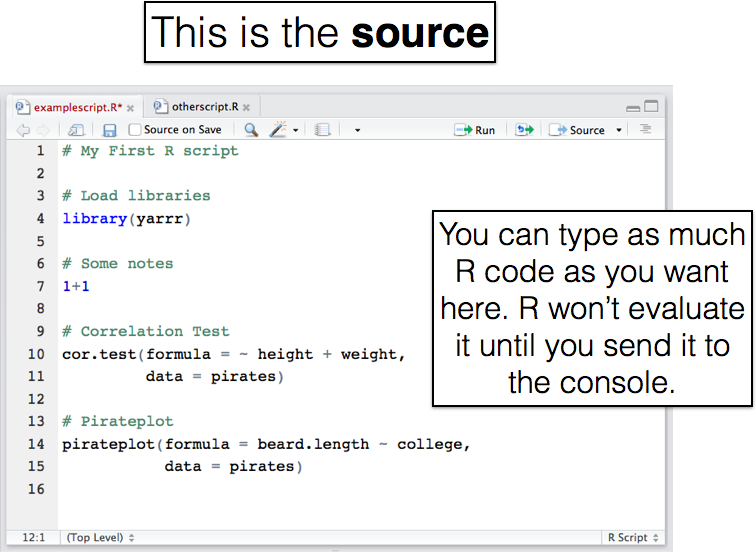
\includegraphics[width=0.75\linewidth]{images/sourcess} 

}

\caption{Here's how a new script looks in the editor window on RStudio. The code you type won't be executed until you send it to the console.}\label{fig:editor}
\end{figure}

You can have several R scripts open in the source window in separate tabs (like I have above).

\hypertarget{send-code-from-a-source-to-the-console}{%
\subsection{Send code from a source to the console}\label{send-code-from-a-source-to-the-console}}

\begin{figure}

{\centering 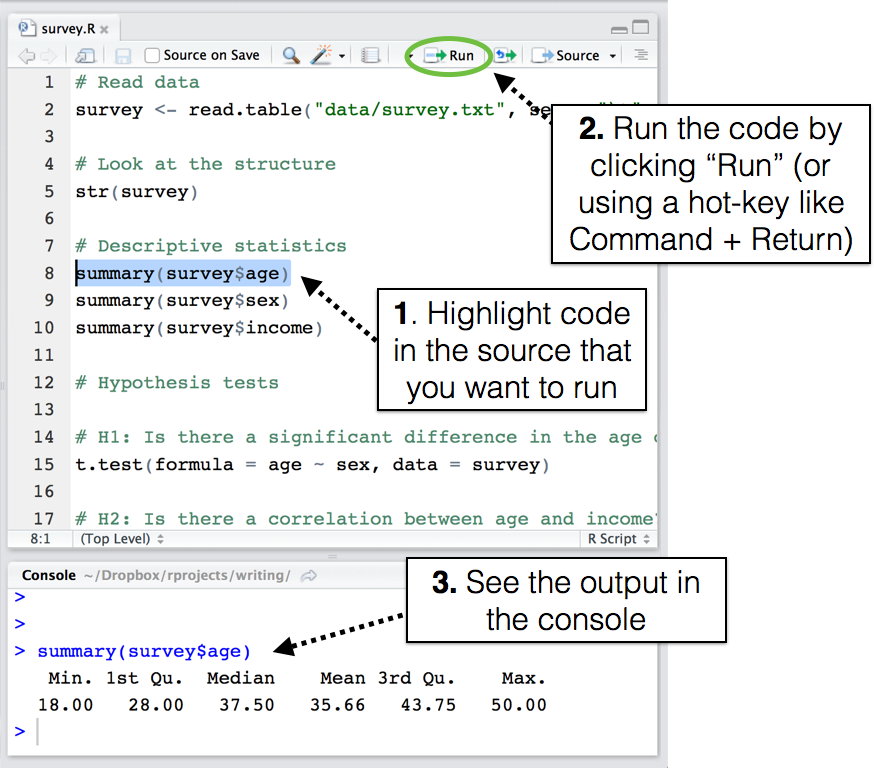
\includegraphics[width=0.75\linewidth]{images/runningcode} 

}

\caption{To evaluate code from the source, highlight it and run it.}\label{fig:runcode}
\end{figure}

When you type code into an R script, you'll notice that, unlike typing code into the Console, nothing happens. In order for R to interpret the code, you need to send it from the Editor to the Console. There are a few ways to do this, here are the three most common ways:

\begin{enumerate}
\def\labelenumi{\arabic{enumi}.}
\item
  Copy (using Crtl+C) the code from the Editor (or anywhere that has valid R code), and paste it into the Console (using Crtl+V).
\item
  Highlight the code you want to run (with your mouse or by holding Shift), then use the Alt+Enter shortcut.
\item
  Place the cursor on a single line you want to run, then use the Alt+Enter shortcut to run just that line.
\end{enumerate}

99\% of the time, I use method 2, where I highlight the code I want, then use the Command--Return shortcut . However, method 3 is great for trouble-shooting code line-by-line.

\hypertarget{writing-r-scripts-using-notebooks}{%
\section{Writing R scripts using notebooks}\label{writing-r-scripts-using-notebooks}}

To start writing a new R notebook in RStudio, in the \texttt{+} image under File, click on it and you should see an image below.

\begin{figure}

{\centering 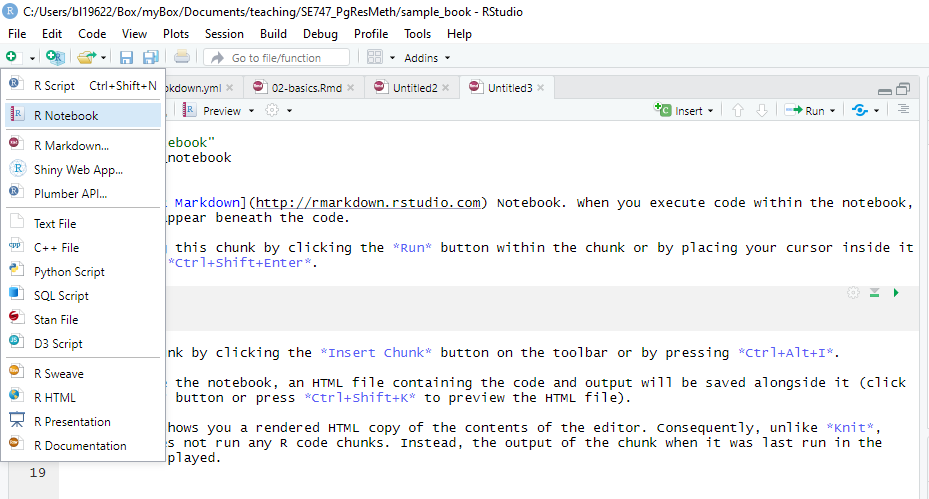
\includegraphics[width=0.75\linewidth]{images/new_notebook} 

}

\caption{How to create a new notebook.}\label{fig:newnotebook}
\end{figure}

Click on \texttt{R\ Notebook} and you should see a blank notebook. What you see in the image below is a new notebook. A notebook is a special type of script that allows you to view the results below the code. As you can see, there are instructions that tells you how to function in a notebook.

\begin{figure}

{\centering 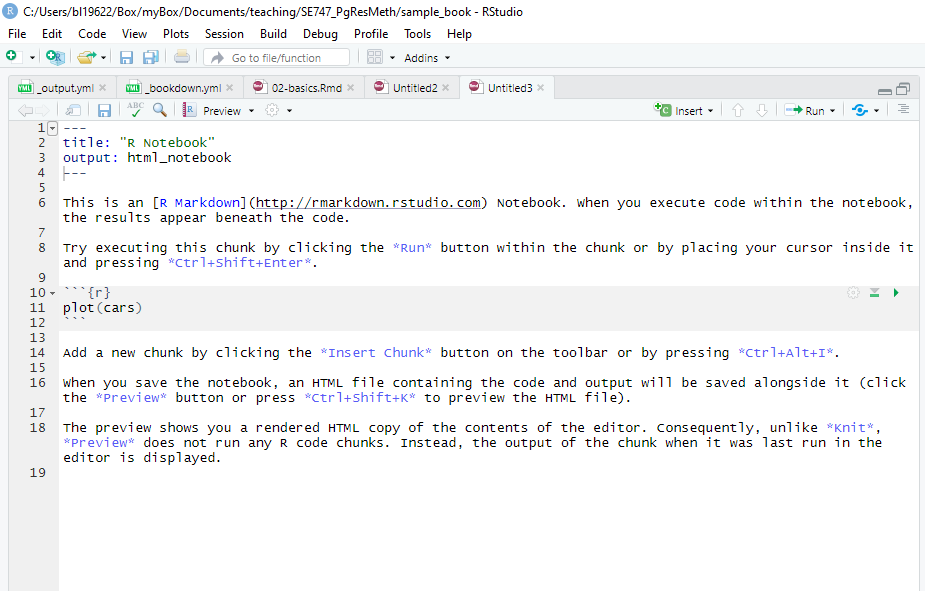
\includegraphics[width=0.75\linewidth]{images/notebook_in_source} 

}

\caption{What a notebook looks like.}\label{fig:notebookview}
\end{figure}

The notebook is a very systematic way of analysing your data, because you can add comments before the code chunk (reminding you of what you did), keep the codes you painfully typed out, and see the results below. You can add more code chunks by pressing the \texttt{Insert} button and selecting the \texttt{R} option. \textbf{I recommend this way of working.}

\begin{figure}

{\centering 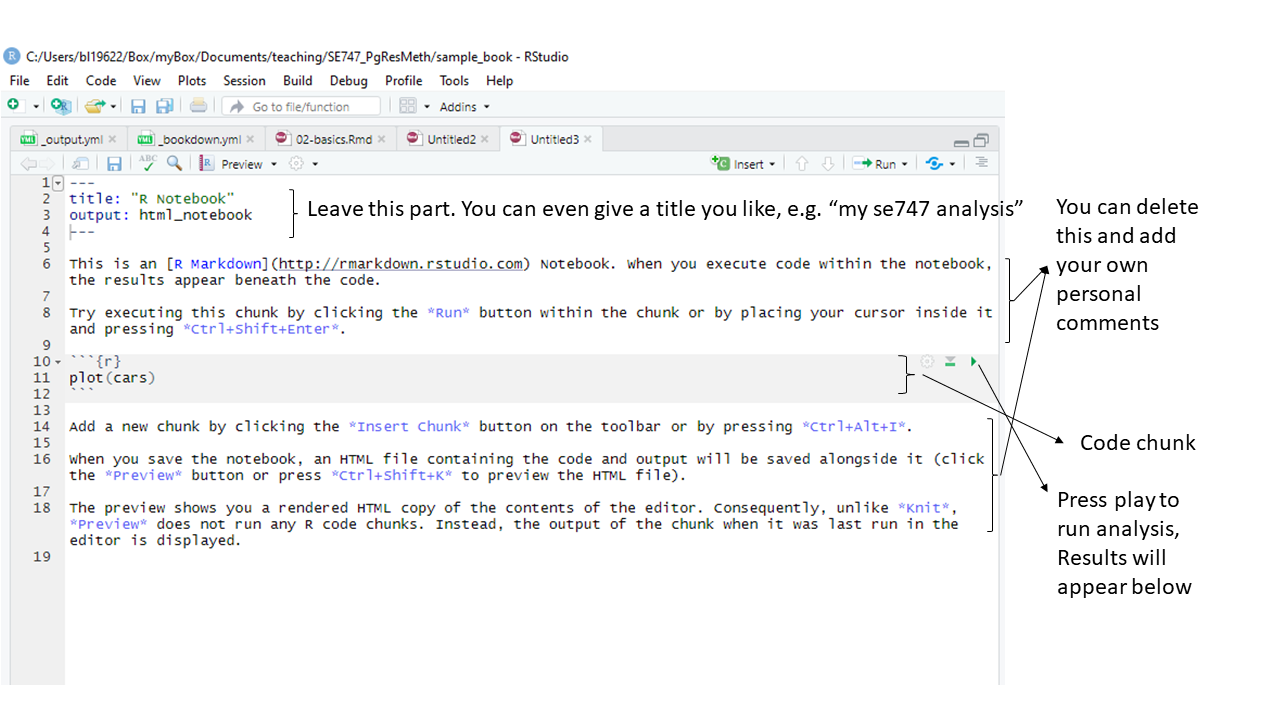
\includegraphics[width=0.75\linewidth]{images/notebook_instruc} 

}

\caption{How to work in a notebook }\label{fig:notebookinstruc}
\end{figure}

\hypertarget{a-brief-style-guide-commenting-and-spacing}{%
\section{A brief style guide: Commenting and spacing}\label{a-brief-style-guide-commenting-and-spacing}}

Like all programming languages, R isn't just meant to be read by a computer, it's also meant to be read by other humans -- or very well-trained dolphins. For this reason, it's important that your code looks nice and is understandable to other people and your future self. To keep things brief, I won't provide a complete style guide -- instead I'll focus on the two most critical aspects of good style: commenting and spacing.

\begin{figure}

{\centering 
\includegraphics[width=0.5\linewidth]{images/futureself} 

}

\caption{As Stan discovered in season six of South Park, your future self is a lazy, possibly intoxicated moron. So do your future self a favor and make your code look nice. Also maybe go for a run once in a while.}\label{fig:futureself}
\end{figure}

\hypertarget{commenting-code-with-the-pound-sign}{%
\subsection{Commenting code with the \# (pound) sign}\label{commenting-code-with-the-pound-sign}}

Comments are completely ignored by R and are just there for whomever is reading the code. You can use comments to explain what a certain line of code is doing, or just to visually separate meaningful chunks of code from each other. Comments in R are designated by a \# (pound) sign. Whenever R encounters a \# sign, it will ignore \textbf{all} the code after the \# sign on that line. Additionally, in most coding editors (like RStudio) the editor will display comments in a separate color than standard R code to remind you that it's a comment:

Here is an example of a short script that is nicely commented. Try to make your scripts look like this!

\begin{Shaded}
\begin{Highlighting}[]
\CommentTok{# Author: Pirate Jack}
\CommentTok{# Title: My nicely commented R Script}
\CommentTok{# Date: None today :(}

\CommentTok{# Step 1: Load the yarrr package}
\KeywordTok{library}\NormalTok{(yarrr)}

\CommentTok{# Step 2: See the column names in the movies dataset}
\KeywordTok{names}\NormalTok{(movies)}

\CommentTok{# Step 3: Calculations}

\CommentTok{# What percent of movies are sequels?}
\KeywordTok{mean}\NormalTok{(movies}\OperatorTok{$}\NormalTok{sequel, }\DataTypeTok{na.rm =}\NormalTok{ T)}

\CommentTok{# How much did Pirate's of the Caribbean: On Stranger Tides make?}
\NormalTok{movies}\OperatorTok{$}\NormalTok{revenue.all[movies}\OperatorTok{$}\NormalTok{name }\OperatorTok{==}\StringTok{ 'Pirates of the Caribbean: On Stranger Tides'}\NormalTok{]}
\end{Highlighting}
\end{Shaded}

I cannot stress enough how important it is to comment your code! Trust me, even if you don't plan on sharing your code with anyone else, keep in mind that your future self will be reading it in the future.

\hypertarget{spacing}{%
\subsection{Spacing}\label{spacing}}

Howwouldyouliketoreadabookiftherewerenospacesbetweenwords?
I'mguessingyouwouldn't.
Soeverytimeyouwritecodewithoutproperspacing,rememberthissentence.

Commenting isn't the only way to make your code legible. It's important to make appropriate use of spaces and line breaks. For example, I include spaces between arithmetic operators (like =, + and -) and after commas (which we'll get to later). For example, look at the following code:

\begin{figure}

{\centering 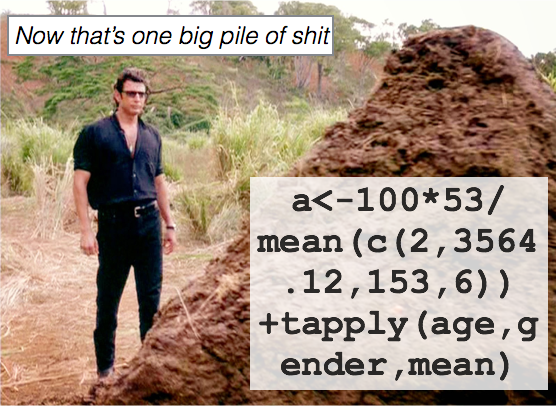
\includegraphics[width=0.5\linewidth]{images/pileofshit} 

}

\caption{Don't make your code look like what a sick Triceratops with diarrhea left behind for Jeff Goldblum.}\label{fig:pileofshit}
\end{figure}

\begin{Shaded}
\begin{Highlighting}[]
\CommentTok{# Shitty looking code}
\NormalTok{a<-(}\DecValTok{100}\OperatorTok{+}\DecValTok{3}\NormalTok{)}\OperatorTok{-}\DecValTok{2}
\KeywordTok{mean}\NormalTok{(}\KeywordTok{c}\NormalTok{(a}\OperatorTok{/}\DecValTok{100}\NormalTok{,}\FloatTok{642564624.34}\NormalTok{))}
\KeywordTok{t.test}\NormalTok{(}\DataTypeTok{formula=}\NormalTok{revenue.all}\OperatorTok{~}\NormalTok{sequel,}\DataTypeTok{data=}\NormalTok{movies)}
\KeywordTok{plot}\NormalTok{(}\DataTypeTok{x=}\NormalTok{movies}\OperatorTok{$}\NormalTok{budget,}\DataTypeTok{y=}\NormalTok{movies}\OperatorTok{$}\NormalTok{dvd.usa,}\DataTypeTok{main=}\StringTok{"myplot"}\NormalTok{)}
\end{Highlighting}
\end{Shaded}

That code looks like shit. Don't write code like that. It makes my eyes hurt. Now, let's use some liberal amounts of commenting and spacing to make it look less shitty.

\begin{Shaded}
\begin{Highlighting}[]
\CommentTok{# Some meaningless calculations. Not important}

\NormalTok{a <-}\StringTok{ }\NormalTok{(}\DecValTok{100} \OperatorTok{+}\StringTok{ }\DecValTok{3}\NormalTok{) }\OperatorTok{-}\StringTok{ }\DecValTok{2}
\KeywordTok{mean}\NormalTok{(}\KeywordTok{c}\NormalTok{(a }\OperatorTok{/}\StringTok{ }\DecValTok{100}\NormalTok{, }\FloatTok{642564624.34}\NormalTok{))}

\CommentTok{# t.test comparing revenue of sequels v non-sequels}

\KeywordTok{t.test}\NormalTok{(}\DataTypeTok{formula =}\NormalTok{ revenue.all }\OperatorTok{~}\StringTok{ }\NormalTok{sequel,}
       \DataTypeTok{data =}\NormalTok{ movies)}

\CommentTok{# A scatterplot of budget and dvd revenue. }
\CommentTok{#  Hard to see a relationship}

\KeywordTok{plot}\NormalTok{(}\DataTypeTok{x =}\NormalTok{ movies}\OperatorTok{$}\NormalTok{budget,}
     \DataTypeTok{y =}\NormalTok{ movies}\OperatorTok{$}\NormalTok{dvd.usa,}
     \DataTypeTok{main =} \StringTok{"myplot"}\NormalTok{)}
\end{Highlighting}
\end{Shaded}

See how much better that second chunk of code looks? Not only do the comments tell us the purpose behind the code, but there are spaces and line-breaks separating distinct elements.

\hypertarget{objects-and-functions}{%
\section{Objects and functions}\label{objects-and-functions}}

To understand how R works, you need to know that R revolves around two things: objects and functions. Almost everything in R is either an object or a function. In the following code chunk, I'll define a simple object called \texttt{tattoos} using a function \texttt{c()}:

\begin{Shaded}
\begin{Highlighting}[]
\CommentTok{# 1: Create a vector object called tattoos}
\NormalTok{tattoos <-}\StringTok{ }\KeywordTok{c}\NormalTok{(}\DecValTok{4}\NormalTok{, }\DecValTok{67}\NormalTok{, }\DecValTok{23}\NormalTok{, }\DecValTok{4}\NormalTok{, }\DecValTok{10}\NormalTok{, }\DecValTok{35}\NormalTok{)}

\CommentTok{# 2: Apply the mean() function to the tattoos object}
\KeywordTok{mean}\NormalTok{(tattoos)}
\end{Highlighting}
\end{Shaded}

\begin{verbatim}
## [1] 23.83333
\end{verbatim}

What is an object? An object is a thing -- like a number, a dataset, a summary statistic like a mean or standard deviation, or a statistical test. Objects come in many different shapes and sizes in R. There are simple objects like \textit{scalars} which represent single numbers, \textbf{vectors} (like our \texttt{tattoos} object above) which represent several numbers, more complex objects like \textbf{dataframes} which represent tables of data, and even more complex objects like \textbf{hypothesis tests} or \textbf{regression} which contain all sorts of statistical information.

Different types of objects have different \emph{attributes}. For example, a vector of data has a length attribute (i.e.; how many numbers are in the vector), while a hypothesis test has many attributes such as a test-statistic and a p-value. Don't worry if this is a bit confusing now -- it will all become clearer when you meet these new objects in person in later chapters. For now, just know that objects in R are things, and different objects have different attributes.

What is a function? A function is a \emph{procedure} that typically takes one or more objects as arguments (aka, inputs), does something with those objects, then returns a new object. For example, the \texttt{mean()} function we used above takes a vector object, like \texttt{tattoos}, of numeric data as an argument, calculates the arithmetic mean of those data, then returns a single number (a scalar) as a result.A great thing about R is that you can easily create your own functions that do whatever you want -- but we'll get to that much later in the book. Thankfully, R has hundreds (thousands?) of built-in functions that perform most of the basic analysis tasks you can think of.

99\% of the time you are using R, you will do the following: 1) Define objects. 2) Apply functions to those objects. 3) Repeat!. Seriously, that's about it. However, as you'll soon learn, the hard part is knowing how to define objects they way you want them, and knowing which function(s) will accomplish the task you want for your objects.

\hypertarget{numbers-versus-characters}{%
\subsection{Numbers versus characters}\label{numbers-versus-characters}}

For the most part, objects in R come in one of two flavors: \textbf{numeric} and \textbf{character}. It is very important to keep these two separate as certain functions, like \texttt{mean()}, and \texttt{max()} will only work for numeric objects, while functions like \texttt{grep()} and \texttt{strtrim()} only work for character objects.

A numeric object is just a number like \texttt{1}, \texttt{10} or \texttt{3.14}. You don't have to do anything special to create a numeric object, just type it like you were using a calculator.

\begin{Shaded}
\begin{Highlighting}[]
\CommentTok{# These are all numeric objects}
\DecValTok{1}
\DecValTok{10}
\FloatTok{3.14}
\end{Highlighting}
\end{Shaded}

A \textbf{character} object is a name like \texttt{"Madisen"}, \texttt{"Brian"}, or \texttt{"University\ of\ Konstanz"}. To specify a character object, you need to include quotation marks \texttt{""} around the text.

\begin{Shaded}
\begin{Highlighting}[]
\CommentTok{# These are all character objects}
\StringTok{"Madisen"}
\StringTok{"Brian"}
\StringTok{"10"}
\end{Highlighting}
\end{Shaded}

If you try to perform a function or operation meant for a numeric object on a character object (and vice-versa), R will yell at you. For example, here's what happens when I try to take the mean of the two character objects \texttt{"1"} and \texttt{"10"}:

\begin{Shaded}
\begin{Highlighting}[]
\CommentTok{# This will return an error because the arguments are not numeric!}
\KeywordTok{mean}\NormalTok{(}\KeywordTok{c}\NormalTok{(}\StringTok{"1"}\NormalTok{, }\StringTok{"10"}\NormalTok{))}
\end{Highlighting}
\end{Shaded}

\begin{error}

Warning message: argument is not numeric or logical, returning NA

\end{error}

If I make sure that the arguments are numeric (by not including the quotation marks), I won't receive the error:

\begin{Shaded}
\begin{Highlighting}[]
\CommentTok{# This is ok!}
\KeywordTok{mean}\NormalTok{(}\KeywordTok{c}\NormalTok{(}\DecValTok{1}\NormalTok{, }\DecValTok{10}\NormalTok{))}
\end{Highlighting}
\end{Shaded}

\begin{verbatim}
## [1] 5.5
\end{verbatim}

\hypertarget{creating-new-objects-with--}{%
\subsection{Creating new objects with \textless-}\label{creating-new-objects-with--}}

By now you know that you can use R to do simple calculations. But to really take advantage of R, you need to know how to create and manipulate objects. All of the data, analyses, and even plots, you use and create are, or can be, saved as objects in R. For example the \texttt{movies} dataset which we've used before is an object stored in the \texttt{yarrr} package. This object was defined in the \texttt{yarrr} package with the name \texttt{movies}. When you loaded the \texttt{yarrr} package with the \texttt{library(\textquotesingle{}yarrr\textquotesingle{})} command, you told R to give you access to the \texttt{movies} object. Once the object was loaded, we could use it to calculate descriptive statistics, hypothesis tests, and to create plots.

To create new objects in R, you need to do \emph{object assignment}. Object assignment is our way of storing information, such as a number or a statistical test, into something we can easily refer to later. This is a pretty big deal. Object assignment allows us to store data objects under relevant names which we can then use to slice and dice specific data objects anytime we'd like to.

To do an assignment, we use the almighty \texttt{\textless{}-} operator called \emph{assign} To assign something to a new object (or to change an existing object), use the notation \texttt{object\ \textless{}-\ ...}\}, where \texttt{object} is the new (or updated) object, and \texttt{...} is whatever you want to store in \texttt{object}. Let's start by creating a very simple object called \texttt{a} and assigning the value of 100 to it:

Good object names strike a balance between being easy to type (i.e.; short names) and interpret. If you have several datasets, it's probably not a good idea to name them \texttt{a}, \texttt{b}, \texttt{c} because you'll forget which is which. However, using long names like \texttt{March2015Group1OnlyFemales} will give you carpal tunnel syndrome.

\begin{Shaded}
\begin{Highlighting}[]
\CommentTok{# Create a new object called a with a value of 100}
\NormalTok{a <-}\StringTok{ }\DecValTok{100}
\end{Highlighting}
\end{Shaded}

Once you run this code, you'll notice that R doesn't tell you anything. However, as long as you didn't type something wrong, R should now have a new object called \texttt{a} which contains the number 100. If you want to see the value, you need to call the object by just executing its name. This will print the value of the object to the console:

\begin{Shaded}
\begin{Highlighting}[]
\CommentTok{# Print the object a}
\NormalTok{a}
\end{Highlighting}
\end{Shaded}

\begin{verbatim}
## [1] 100
\end{verbatim}

Now, R will print the value of \texttt{a} (in this case 100) to the console. If you try to evaluate an object that is not yet defined, R will return an error. For example, let's try to print the object \texttt{b} which we haven't yet defined:

\begin{Shaded}
\begin{Highlighting}[]
\NormalTok{b}
\end{Highlighting}
\end{Shaded}

\begin{error}

Error: object `b' not found

\end{error}

As you can see, R yelled at us because the object \texttt{b} hasn't been defined yet.

Once you've defined an object, you can combine it with other objects using basic arithmetic. Let's create objects \texttt{a} and \texttt{b} and play around with them.

\begin{Shaded}
\begin{Highlighting}[]
\NormalTok{a <-}\StringTok{ }\DecValTok{1}
\NormalTok{b <-}\StringTok{ }\DecValTok{100}

\CommentTok{# What is a + b?}
\NormalTok{a }\OperatorTok{+}\StringTok{ }\NormalTok{b}
\end{Highlighting}
\end{Shaded}

\begin{verbatim}
## [1] 101
\end{verbatim}

\begin{Shaded}
\begin{Highlighting}[]
\CommentTok{# Assign a + b to a new object (c)}
\NormalTok{c <-}\StringTok{ }\NormalTok{a }\OperatorTok{+}\StringTok{ }\NormalTok{b}

\CommentTok{# What is c?}
\NormalTok{c}
\end{Highlighting}
\end{Shaded}

\begin{verbatim}
## [1] 101
\end{verbatim}

\hypertarget{to-change-an-object-you-must-assign-it-again}{%
\subsubsection{To change an object, you must assign it again!}\label{to-change-an-object-you-must-assign-it-again}}

Normally I try to avoid excessive emphasis, but because this next sentence is so important, I have to just go for it. Here it goes\ldots{}

\textbf{To change an object, you \textit{must} assign it again!}

No matter what you do with an object, if you don't assign it again, it won't change. For example, let's say you have an object \texttt{z} with a value of 0. You'd like to add 1 to \texttt{z} in order to make it 1. To do this, you might want to just enter \texttt{z\ +\ 1} -- but that won't do the job. Here's what happens if you \textbf{don't} assign it again:

\begin{Shaded}
\begin{Highlighting}[]
\NormalTok{z <-}\StringTok{ }\DecValTok{0}
\NormalTok{z }\OperatorTok{+}\StringTok{ }\DecValTok{1}
\end{Highlighting}
\end{Shaded}

\begin{verbatim}
## [1] 1
\end{verbatim}

Ok! Now let's see the value of \texttt{z}

\begin{Shaded}
\begin{Highlighting}[]
\NormalTok{z}
\end{Highlighting}
\end{Shaded}

\begin{verbatim}
## [1] 0
\end{verbatim}

Damn! As you can see, the value of z is still 0! What went wrong? Oh yeah\ldots{}

\textbf{To change an object, you \emph{must} assign it again!}

The problem is that when we wrote \texttt{z\ +\ 1} on the second line, R thought we just wanted it to calculate and print the value of \texttt{z\ +\ 1}, without storing the result as a new \texttt{z} object. If we want to actually update the value of \texttt{z}, we need to reassign the result back to \texttt{z} as follows:

\begin{Shaded}
\begin{Highlighting}[]
\NormalTok{z <-}\StringTok{ }\DecValTok{0}
\NormalTok{z <-}\StringTok{ }\NormalTok{z }\OperatorTok{+}\StringTok{ }\DecValTok{1}  \CommentTok{# Now I'm REALLY changing z}
\NormalTok{z}
\end{Highlighting}
\end{Shaded}

\begin{verbatim}
## [1] 1
\end{verbatim}

Phew, z is now 1. Because we used assignment, z has been updated. About freaking time.

\hypertarget{how-to-name-objects}{%
\subsection{How to name objects}\label{how-to-name-objects}}

You can create object names using any combination of letters and a few special characters (like \texttt{.} and \texttt{\_}). Here are some valid object names

\begin{Shaded}
\begin{Highlighting}[]
\CommentTok{# Valid object names}
\NormalTok{group.mean <-}\StringTok{ }\FloatTok{10.21}
\NormalTok{my.age <-}\StringTok{ }\DecValTok{32}
\NormalTok{FavoritePirate <-}\StringTok{ "Jack Sparrow"}
\NormalTok{sum.}\FloatTok{1.}\NormalTok{to}\FloatTok{.5}\NormalTok{ <-}\StringTok{ }\DecValTok{1} \OperatorTok{+}\StringTok{ }\DecValTok{2} \OperatorTok{+}\StringTok{ }\DecValTok{3} \OperatorTok{+}\StringTok{ }\DecValTok{4} \OperatorTok{+}\StringTok{ }\DecValTok{5}
\end{Highlighting}
\end{Shaded}

All the object names above are perfectly valid. Now, let's look at some examples of \emph{invalid} object names. These object names are all invalid because they either contain spaces, start with numbers, or have invalid characters:

\begin{Shaded}
\begin{Highlighting}[]
\CommentTok{# Invalid object names!}
\NormalTok{famale ages <-}\StringTok{ }\DecValTok{50} \CommentTok{# spaces}
\NormalTok{5experiment <-}\StringTok{ }\DecValTok{50} \CommentTok{# starts with a number}
\NormalTok{a}\OperatorTok{!}\StringTok{ }\ErrorTok{<}\OperatorTok{-}\StringTok{ }\DecValTok{50} \CommentTok{# has an invalid character}
\end{Highlighting}
\end{Shaded}

If you try running the code above in R, you will receive a warning message starting with

\begin{error}

Error: unexpected symbol

\end{error}

. Anytime you see this warning in R, it almost always means that you have a naming error of some kind.

\hypertarget{r-is-case-sensitive}{%
\subsubsection{R is case-sensitive!}\label{r-is-case-sensitive}}

\begin{figure}

{\centering 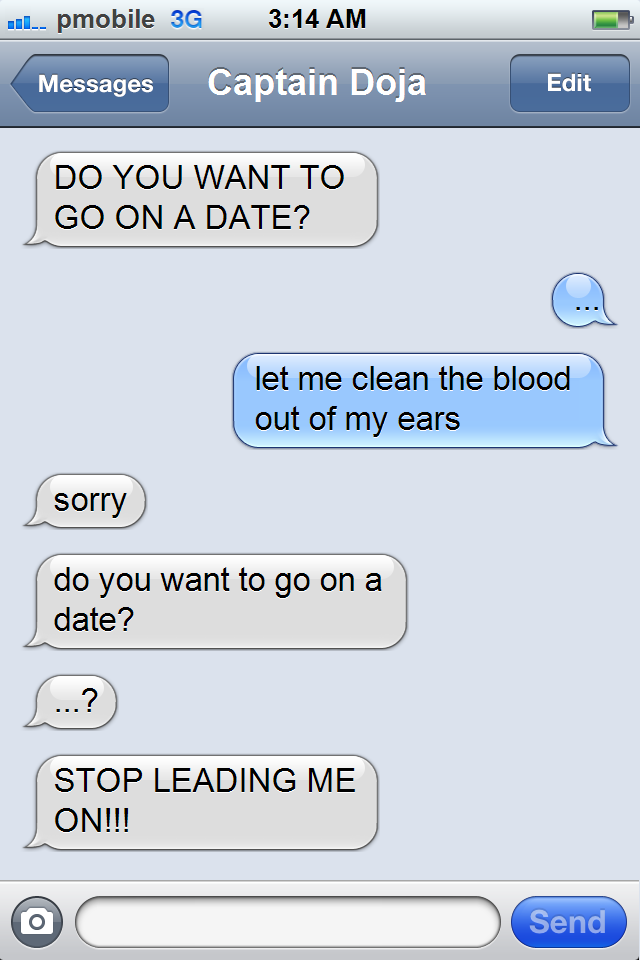
\includegraphics[width=0.5\linewidth]{images/datetext} 

}

\caption{Like a text message, you should probably watch your use of capitalization in R.}\label{fig:datetext}
\end{figure}

Like English, R is case-sensitive -- it R treats capital letters differently from lower-case letters. For example, the four following objects \texttt{Plunder}, \texttt{plunder} and \texttt{PLUNDER} are totally different objects in R:

\begin{Shaded}
\begin{Highlighting}[]
\CommentTok{# These are all different objects}
\NormalTok{Plunder <-}\StringTok{ }\DecValTok{1}
\NormalTok{plunder <-}\StringTok{ }\DecValTok{100}
\NormalTok{PLUNDER <-}\StringTok{ }\DecValTok{5}
\end{Highlighting}
\end{Shaded}

I try to avoid using too many capital letters in object names because they require me to hold the shift key. This may sound silly, but you'd be surprised how much easier it is to type \texttt{mydata} than \texttt{MyData} 100 times.

\#\#\#Example: Pirates of The Caribbean

Let's do a more practical example -- we'll define an object called \texttt{blackpearl.usd} which has the global revenue of Pirates of the Caribbean: Curse of the Black Pearl in U.S. dollars. A quick Google search showed me that the revenue was \$634,954,103. I'll create the new object using assignment:

\begin{Shaded}
\begin{Highlighting}[]
\NormalTok{blackpearl.usd <-}\StringTok{ }\DecValTok{634954103}
\end{Highlighting}
\end{Shaded}

Now, my fellow European pirates might want to know how much this is in Euros. Let's create a new object called \texttt{\{blackpearl.eur} which converts our original value to Euros by multiplying the original amount by 0.88 (assuming 1 USD = 0.88 EUR)

\begin{Shaded}
\begin{Highlighting}[]
\NormalTok{blackpearl.eur <-}\StringTok{ }\NormalTok{blackpearl.usd }\OperatorTok{*}\StringTok{ }\FloatTok{0.88}
\NormalTok{blackpearl.eur}
\end{Highlighting}
\end{Shaded}

\begin{verbatim}
## [1] 558759611
\end{verbatim}

It looks like the movie made 558,759,611 in Euros. Not bad. Now, let's see how much more Pirates of the Caribbean 2: Dead Man's Chest made compared to ``Curse of the Black Pearl.'' Another Google search uncovered that Dead Man's Chest made \$1,066,215,812 (that wasn't a mistype, the freaking movie made over a billion dollars).

\begin{Shaded}
\begin{Highlighting}[]
\NormalTok{deadman.usd <-}\StringTok{ }\DecValTok{1066215812}
\end{Highlighting}
\end{Shaded}

Now, I'll divide \texttt{deadman.usd} by \texttt{blackpearl.usd}:

\begin{Shaded}
\begin{Highlighting}[]
\NormalTok{deadman.usd }\OperatorTok{/}\StringTok{ }\NormalTok{blackpearl.usd}
\end{Highlighting}
\end{Shaded}

\begin{verbatim}
## [1] 1.679201
\end{verbatim}

It looks like ``Dead Man's Chest'' made 168\% as much as ``Curse of the Black Pearl'' - not bad for two movies based off of a ride from Disneyland.

\hypertarget{NavigatingTheSoftware}{%
\chapter{Navigating the Software}\label{NavigatingTheSoftware}}

\hypertarget{introduction}{%
\section*{Introduction}\label{introduction}}
\addcontentsline{toc}{section}{Introduction}

Both R and RStudio are big chunks of software, first and foremost. You will inevitably
spend time doing what one does with any big piece of software:
configuring it, customizing it, updating it, and fitting it into your
computing environment. This chapter will help you perform those tasks.
There is nothing here about numerics, statistics, or graphics. This is
all about dealing with R and RStudio as software.

\hypertarget{download-and-load-libraries}{%
\section*{Download and load libraries}\label{download-and-load-libraries}}
\addcontentsline{toc}{section}{Download and load libraries}

\begin{Shaded}
\begin{Highlighting}[]
\ControlFlowTok{if}\NormalTok{ (}\OperatorTok{!}\KeywordTok{require}\NormalTok{(}\StringTok{"pacman"}\NormalTok{)) }\KeywordTok{install.packages}\NormalTok{(}\StringTok{"pacman"}\NormalTok{)}
\NormalTok{pacman}\OperatorTok{::}\KeywordTok{p_load}\NormalTok{(tidyverse, }\CommentTok{# All purpose wrangling for dataframes}
\NormalTok{               readr, }\CommentTok{# importing and writing data}
\NormalTok{               readxl,}\CommentTok{# read and write excel documents}
\NormalTok{               purrr, }\CommentTok{# for piping %>%}
\NormalTok{               corrplot, }\CommentTok{# for correlation}
\NormalTok{               knitr,}
\NormalTok{               yarrr)}
\end{Highlighting}
\end{Shaded}

\begin{figure}

{\centering 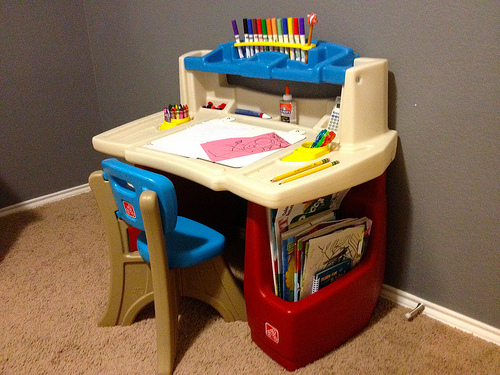
\includegraphics[width=0.75\linewidth]{images/workspace} 

}

\caption{Your workspace -- all the objects, functions, and delicious glue you've defined in your current session.}\label{fig:workspace}
\end{figure}

Remember way back in Chapter 2 when I said everything in R is an object? Well, that's still true. In this chapter, we'll cover the basics of R object management. We'll cover how to load new objects like external datasets into R, how to manage the objects that you already have, and how to export objects from R into external files that you can share with other people or store for your own future use.

\hypertarget{getting-and-setting-the-working-directory}{%
\section{Getting and Setting the Working Directory}\label{getting-and-setting-the-working-directory}}

Your computer is a maze of folders, files. Outside of R, when you want to open a specific file, you probably open up an explorer window that allows you to visually search through the folders on your computer. Or, maybe you select recent files, or type the name of the file in a search box to let your computer do the searching for you. While this system usually works for non-programming tasks, it is a no-go for R. Why? Well, the main problem is that all of these methods require you to \emph{visually} scan your folders and move your mouse to select folders and files that match what you are looking for. When you are programming in R, you need to specify \emph{all} steps in your analyses in a way that can be easily replicated by others and your future self. This means you can't just say: ``Find this one file I emailed to myself a week ago'' or ``Look for a file that looks something like \texttt{experimentAversion3.txt}.'' Instead, need to be able to write R code that tells R \emph{exactly} where to find critical files -- either on your computer or on the web.

To make this job easier, R uses \textbf{working directories}.

You want to change your working directory, or you just want to know what
it is.

\begin{description}
\item[RStudio]
Navigate to a directory in the Files pane. Then from the Files pane, select More → Set As Working Directory, as shown in Figure \ref{fig:workingdir}.
\end{description}

\begin{figure}
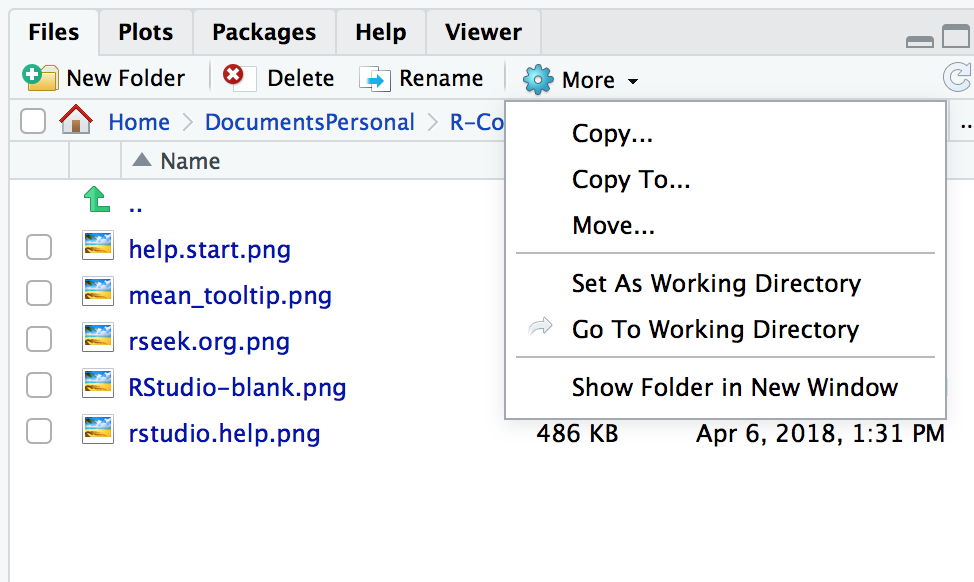
\includegraphics[width=13.53in]{images/rstudio.files} \caption{RStudio: Set As Working Directory}\label{fig:workingdir}
\end{figure}

\begin{description}
\item[Console]
Use \texttt{getwd} to report the working directory, and use \texttt{setwd} to
change it:
\end{description}

\begin{Shaded}
\begin{Highlighting}[]
\KeywordTok{getwd}\NormalTok{()}
\end{Highlighting}
\end{Shaded}

\begin{verbatim}
## [1] "C:/Users/liew_/Box/myBox/Documents/teaching/SE747_PgResMeth/se747_stats_book"
\end{verbatim}

Saving the working directory path into an object called \texttt{currwd}

\begin{Shaded}
\begin{Highlighting}[]
\NormalTok{currwd <-}\StringTok{ }\KeywordTok{getwd}\NormalTok{()}
\end{Highlighting}
\end{Shaded}

\begin{Shaded}
\begin{Highlighting}[]
\CommentTok{# setting it manually with copy + paste}
\KeywordTok{setwd}\NormalTok{(}\StringTok{"C:/Users/bl19622/Box/myBox/Documents/teaching/SE747_PgResMeth/sample_book"}\NormalTok{)}

\CommentTok{#  setting it using the object we created}
\KeywordTok{setwd}\NormalTok{ (currwd)}
\end{Highlighting}
\end{Shaded}

Your working directory is important because it is the default location
for all file input and output---including reading and writing data files,
opening and saving script files, and saving your workspace image. When
you open a file and do not specify an absolute path, R will assume that
the file is in your working directory.

If you're using RStudio projects, your default working directory will be the home directory of the project.

\hypertarget{creating-a-new-rstudio-project}{%
\section{Creating a new Rstudio project}\label{creating-a-new-rstudio-project}}

You want to create a new RStudio project to keep all your files related to a specific project.
Click File → New Project as in Figure \ref{fig:filenew-drop}. ** I ALWAYS use this approach, please use it too**

\begin{figure}
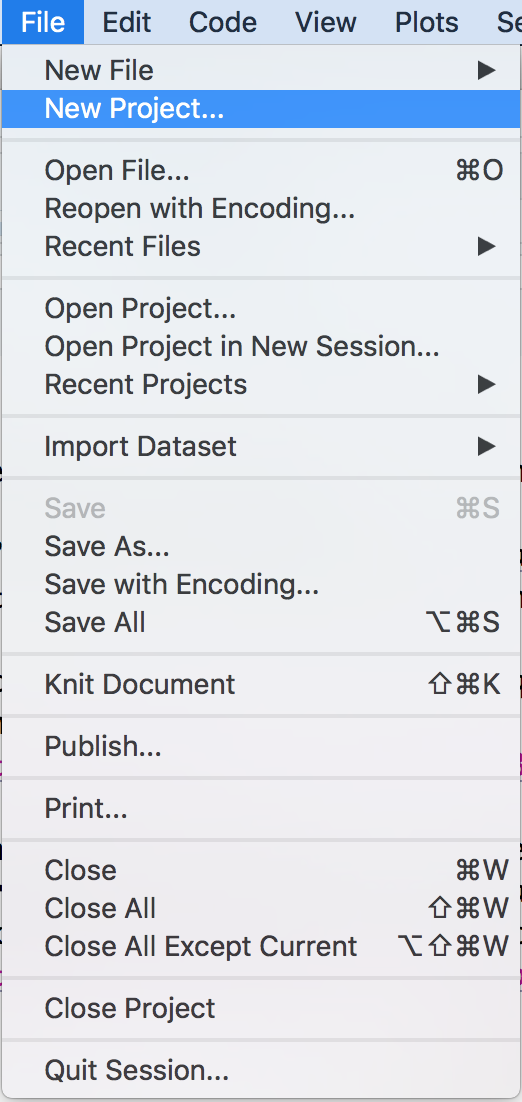
\includegraphics[width=7.25in]{images/rstudio.file.newproject} \caption{Selecting New Project}\label{fig:filenew-drop}
\end{figure}

This will open the New Project dialog box and allow you to choose which type of project you would like to create, as shown in Figure \ref{fig:filenewmenu}.

\begin{figure}
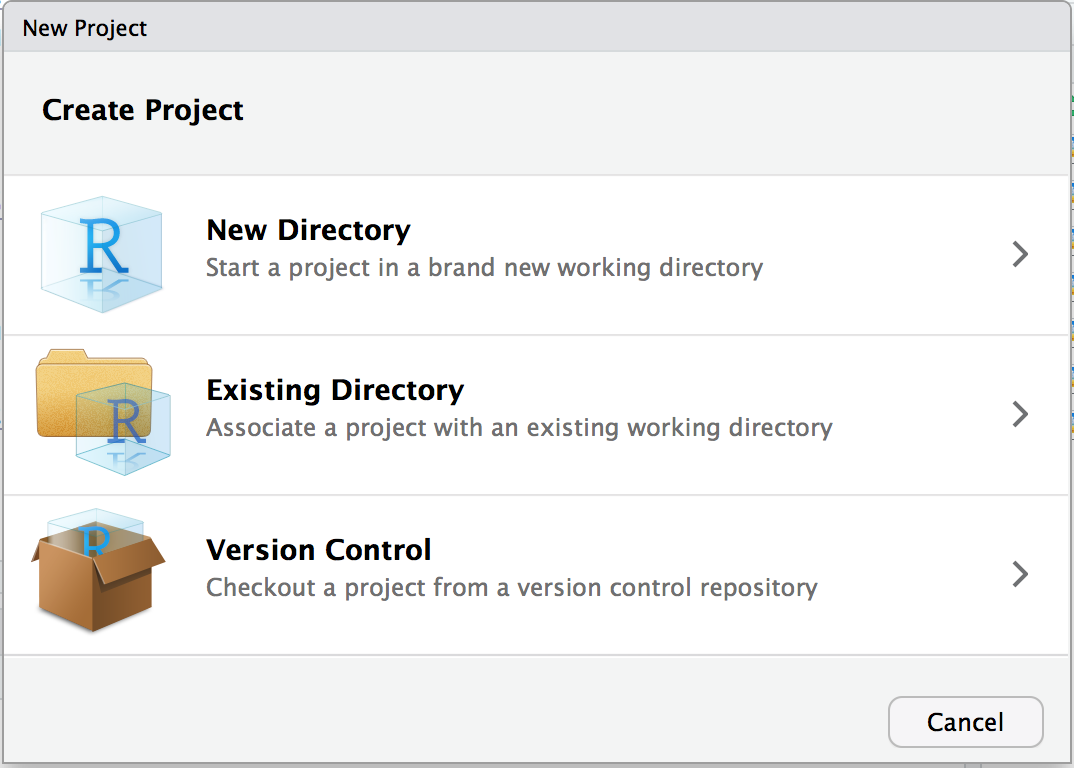
\includegraphics[width=14.92in]{images/rstudio.newproject.dialog} \caption{New Project dialog}\label{fig:filenewmenu}
\end{figure}

Projects are a powerful concept that's specific to RStudio. They help you by doing the following:

\begin{itemize}
\tightlist
\item
  Setting your working directory to the project directory.
\item
  Preserving window state in RStudio so when you return to a project your windows are all as you left them. This includes opening any files you had open when you last saved your project.
\item
  Preserving RStudio project settings.
\end{itemize}

To hold your project settings, RStudio creates a project file with an \emph{.Rproj} extension in the project directory. If you open the project file in RStudio, it works like a shortcut for opening the project. In addition, RStudio creates a hidden directory named \emph{.Rproj.user} to house temporary files related to your project.

Any time you're working on something nontrivial in R we recommend creating an RStudio project. Projects help you stay organized and make your project workflow easier.

\hypertarget{viewing-your-command-history}{%
\section{Viewing Your Command History}\label{viewing-your-command-history}}

You want to see your recent sequence of commands.

Depending on what you are trying to accomplish, you can use a few different methods to access your prior command history. If you are in the RStudio console pane, you can press the up arrow to interactively scroll through past commands.

If you want to see a listing of past commands, you can either execute the \texttt{history}
function or access the History pane in RStudio to view your most recent input:

\begin{Shaded}
\begin{Highlighting}[]
\KeywordTok{history}\NormalTok{()}
\end{Highlighting}
\end{Shaded}

In RStudio typing \texttt{history()} into the console simply activates the History pane in RStudio (Figure \ref{fig:history}). You could also make that pane visible by clicking on it with your cursor.

\begin{figure}
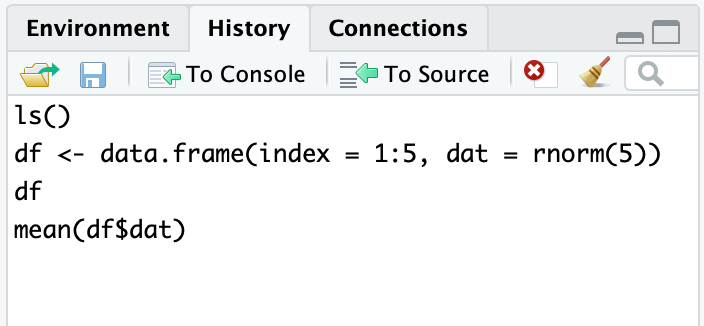
\includegraphics[width=9.78in]{images/history} \caption{RStudio History pane}\label{fig:history}
\end{figure}

The \texttt{history} function displays your most recent commands. In RStudio the \texttt{history} command will activate the History pane. If you were running R outside of RStudio, \texttt{history} shows the most recent 25 lines, but you can request more like so:

\begin{Shaded}
\begin{Highlighting}[]
\KeywordTok{history}\NormalTok{(}\DecValTok{100}\NormalTok{)          }\CommentTok{# Show 100 most recent lines of history}
\KeywordTok{history}\NormalTok{(}\OtherTok{Inf}\NormalTok{)          }\CommentTok{# Show entire saved history}
\end{Highlighting}
\end{Shaded}

From within RStudio, the History tab shows an exhaustive list of past commands in chronological order, with the most recent at the bottom of the list. You can highlight past commands with your cursor, then click on ``To Console'' or ``To Source'' to copy past commands into the console or source editor, respectively. This can be terribly handy when you've done interactive data analysis and then decide you want to save some past steps to a source file for later use.

From the console you can see your history by simply pressing the up arrow to scroll backward through your input, which causes your previous typing to reappear, one line at a time.

If you've exited from R or RStudio, you can still see your command history. R
saves the history in a file called \emph{.Rhistory} in the working directory. Open the file with a text editor and then scroll to the
bottom; you will see your most recent typing.

\hypertarget{installing-packages}{%
\section{Installing Packages}\label{installing-packages}}

When you download and install R for the first time, you are installing the Base R software. Base R will contain most of the functions you'll use on a daily basis like \texttt{mean()} and \texttt{hist()}. However, only functions written by the original authors of the R language will appear here. If you want to access data and code written by other people, you'll need to install it as a \emph{package}. An R package is simply a bunch of data, from functions, to help menus, to vignettes (examples), stored in one neat package.

\begin{figure}

{\centering 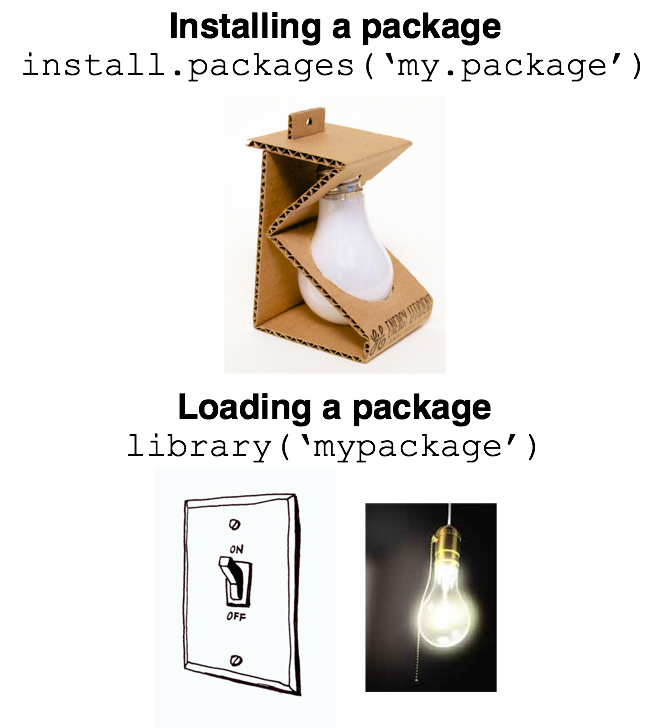
\includegraphics[width=0.5\linewidth]{images/packagebulb} 

}

\caption{An R package is like a lightbulb. First you need to order it with install.packages(). Then, every time you want to use it, you need to turn it on with library()}\label{fig:package}
\end{figure}

A package is like a light bulb. In order to use it, you first need to order it to your house (i.e.; your computer) by \emph{installing} it. Once you've installed a package, you never need to install it again. However, every time you want to actually use the package, you need to turn it on by \emph{loading} it. Here's how to do it.

\hypertarget{installing-a-new-package}{%
\subsection{Installing a new package}\label{installing-a-new-package}}

Installing a package simply means downloading the package code onto your personal computer. There are two main ways to install new packages. The first, and most common, method is to download them from the Comprehensive R Archive Network (CRAN). CRAN is the central repository for R packages. To install a new R package from CRAN, you can simply run the code \texttt{install.packages("name")}, where ``name'' is the name of the package. For example, to download the \texttt{yarrr} package, which contains several data sets and functions we will use in this book, you should run the following:

\begin{figure}

{\centering 
\includegraphics[width=0.5\linewidth]{images/cran} 

}

\caption{CRAN (Comprehensive R Archive Network) is the main source of R packages}\label{fig:cran}
\end{figure}

\begin{Shaded}
\begin{Highlighting}[]
\CommentTok{# Install the yarrr package from CRAN}
\CommentTok{#   You only need to install a package once!}
\KeywordTok{install.packages}\NormalTok{(}\StringTok{"yarrr"}\NormalTok{)}
\end{Highlighting}
\end{Shaded}

When you run \texttt{install.packages("name")} R will download the package from CRAN. If everything works, you should see some information about where the package is being downloaded from, in addition to a progress bar.

\begin{figure}

{\centering 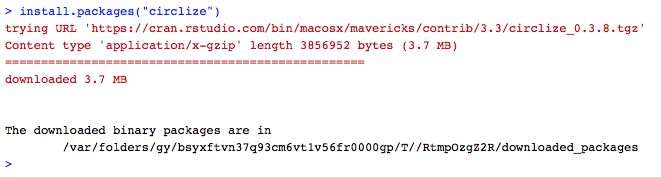
\includegraphics[width=0.75\linewidth]{images/installingpackages} 

}

\caption{When you install a new package, you'll see some random text like this you the download progress. You don't need to memorize this.}\label{fig:installingpackages}
\end{figure}

Like ordering a light bulb, once you've installed a package on your computer you never need to install it again (unless you want to try to install a new version of the package). However, every time you want to use it, you need to turn it on by loading it.

\hypertarget{loading-a-package}{%
\subsection{Loading a package}\label{loading-a-package}}

Once you've installed a package, it's on your computer. However, just because it's on your computer doesn't mean R is ready to use it. If you want to use something, like a function or dataset, from a package you \emph{always} need to \emph{load} the package in your R session first. Just like a light bulb, you need to turn it on to use it!

To load a package, you use the \texttt{library()} function. For example, now that we've installed the \texttt{yarrr} package, we can load it with \texttt{library("yarrr")}:

\begin{Shaded}
\begin{Highlighting}[]
\CommentTok{# Load the yarrr package so I can use it!}
\CommentTok{#   You have to load a package in every new R session!}
\KeywordTok{library}\NormalTok{(}\StringTok{"yarrr"}\NormalTok{)}
\end{Highlighting}
\end{Shaded}

Now that you've loaded the \texttt{yarrr} package, you can use any of its functions! One of the coolest functions in this package is called \texttt{pirateplot()}. Rather than telling you what a pirateplot is, let's just make one. Run the following code chunk to make your own pirateplot. Don't worry about the specifics of the code below, you'll learn more about how all this works later. For now, just run the code and marvel at your pirateplot.

\begin{Shaded}
\begin{Highlighting}[]
\CommentTok{# Make a pirateplot using the pirateplot() function}
\CommentTok{#  from the yarrr package!}

\KeywordTok{pirateplot}\NormalTok{(}\DataTypeTok{formula =}\NormalTok{ weight }\OperatorTok{~}\StringTok{ }\NormalTok{Time, }
           \DataTypeTok{data =}\NormalTok{ ChickWeight,}
           \DataTypeTok{pal =} \StringTok{"xmen"}\NormalTok{)}
\end{Highlighting}
\end{Shaded}

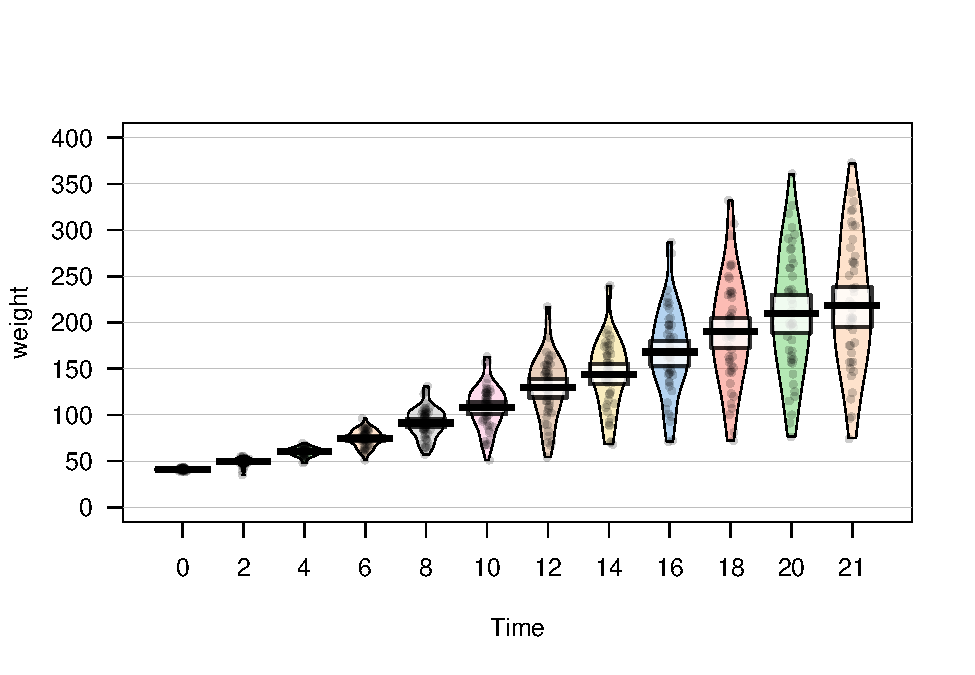
\includegraphics{03-navigatingworkspace_files/figure-latex/unnamed-chunk-9-1.pdf}

There is one way in R to temporarily load a package without using the \texttt{library()} function. To do this, you can simply use the notation \texttt{package::function} notation. This notation simply tells R to load the package just for this one chunk of code. For example, I could use the \texttt{pirateplot} function from \texttt{yarrr} package as follows:

\begin{Shaded}
\begin{Highlighting}[]
\CommentTok{# Use the pirateplot() function without loading the yarrr package first}
\NormalTok{yarrr}\OperatorTok{::}\KeywordTok{pirateplot}\NormalTok{(}\DataTypeTok{formula =}\NormalTok{ weight }\OperatorTok{~}\StringTok{ }\NormalTok{Diet,}
                  \DataTypeTok{data =}\NormalTok{ ChickWeight)}
\end{Highlighting}
\end{Shaded}

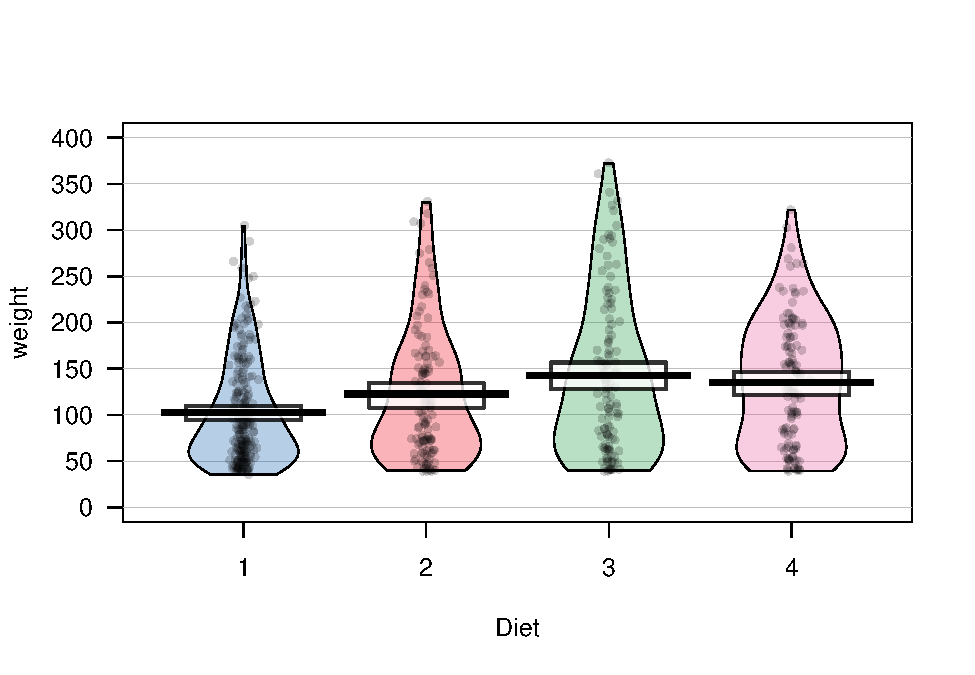
\includegraphics{03-navigatingworkspace_files/figure-latex/unnamed-chunk-10-1.pdf}

Again, you can think about the \texttt{package::function} method as a way to temporarily loading a package for a single line of code. One benefit of using the \texttt{package::function} notation is that it's immediately clear to anyone reading the code which package contains the function. However, a drawback is that if you are using a function from a package often, it forces you to constantly retype the package name. You can use whichever method makes sense for you.

\hypertarget{learning-check}{%
\section*{Learning check}\label{learning-check}}
\addcontentsline{toc}{section}{Learning check}

\begin{enumerate}
\def\labelenumi{\arabic{enumi}.}
\item
  Create a folder called \texttt{se747} on your computer desktop.
\item
  Create a new project in the folder \texttt{se747}, click File -- New Project -- New Directory -- New Project -- Browse, sear for \texttt{se747} folder -- under Directory name, type \texttt{analysis}.
\item
  Create a new R script, click File -- New File -- R Script.
\item
  Save the new R script, click File -- Save As. Use the file name \texttt{new\_script}. It will have the extension \texttt{.R}
\item
  Enter the code below into your new script, and save it.
\end{enumerate}

\begin{Shaded}
\begin{Highlighting}[]
\NormalTok{a <-}\StringTok{ }\DecValTok{10}
\NormalTok{a }\OperatorTok{+}\StringTok{ }\DecValTok{10}
\NormalTok{a}
\end{Highlighting}
\end{Shaded}

\begin{enumerate}
\def\labelenumi{\arabic{enumi}.}
\setcounter{enumi}{5}
\item
  Close RStudio, reopen RStudio. In the Files tab on the bottom right, you should see the script you created \texttt{new\_script.R}. Click on it to open and you should see the code you typed.
\item
  Create a new R notebook, click File -- New File -- R Notebook.
\item
  Save the new R notebook, click File -- Save As. Use the file name \texttt{practice}. It will have the extension \texttt{.Rmd}
\item
  Clear all the default comments after the headers and before the code chunk. Insert the code chunk below in the notebook and type a few comments before the code to remind you what you executed.
\end{enumerate}

\begin{Shaded}
\begin{Highlighting}[]
\ControlFlowTok{if}\NormalTok{ (}\OperatorTok{!}\KeywordTok{require}\NormalTok{(}\StringTok{"pacman"}\NormalTok{)) }\KeywordTok{install.packages}\NormalTok{(}\StringTok{"pacman"}\NormalTok{)}
\NormalTok{pacman}\OperatorTok{::}\KeywordTok{p_load}\NormalTok{(tidyverse, }\CommentTok{# All purpose wrangling for dataframes}
\NormalTok{               readr, }\CommentTok{# importing and writing data}
\NormalTok{               openxlsx) }\CommentTok{# writing excel documents}
\end{Highlighting}
\end{Shaded}

\begin{enumerate}
\def\labelenumi{\arabic{enumi}.}
\setcounter{enumi}{7}
\tightlist
\item
  Remember to save the notebook.
\end{enumerate}

\hypertarget{input-and-output}{%
\chapter{Input and Output}\label{input-and-output}}

\hypertarget{download-and-load-libraries}{%
\section*{Download and load libraries}\label{download-and-load-libraries}}
\addcontentsline{toc}{section}{Download and load libraries}

\begin{Shaded}
\begin{Highlighting}[]
\ControlFlowTok{if}\NormalTok{ (}\OperatorTok{!}\KeywordTok{require}\NormalTok{(}\StringTok{"pacman"}\NormalTok{)) }\KeywordTok{install.packages}\NormalTok{(}\StringTok{"pacman"}\NormalTok{)}
\NormalTok{pacman}\OperatorTok{::}\KeywordTok{p_load}\NormalTok{(tidyverse, }\CommentTok{# All purpose wrangling for dataframes}
\NormalTok{               readr, }\CommentTok{# importing and writing data}
\NormalTok{               openxlsx) }\CommentTok{# writing excel documents}
\end{Highlighting}
\end{Shaded}

\hypertarget{dealing-with-cannot-open-file-in-windows}{%
\section{Dealing with ``Cannot Open File'' in Windows}\label{dealing-with-cannot-open-file-in-windows}}

You are running R on Windows, and you are using filenames such as
\texttt{C:\textbackslash{}data\textbackslash{}sample.txt}. R says it cannot open the file, but you know the
file does exist.

The backslashes in the filepath are causing trouble. You can solve this
problem in one of two ways:

\begin{itemize}
\item
  Change the backslashes to forward slashes: \texttt{"C:/data/sample.txt"}.
\item
  Double the backslashes: \texttt{"C:\textbackslash{}\textbackslash{}data\textbackslash{}\textbackslash{}sample.txt"}.
\end{itemize}

When you open a file in R, you give the filename as a character string.
Problems arise when the name contains backslashes (\texttt{\textbackslash{}}) because
backslashes have a special meaning inside strings. You'll probably get
something like this:

\begin{Shaded}
\begin{Highlighting}[]
\NormalTok{samp <-}\StringTok{ }\KeywordTok{read.table}\NormalTok{(}\StringTok{"data\textbackslash{}STRENGTH.txt"}\NormalTok{)}
\end{Highlighting}
\end{Shaded}

\begin{verbatim}
## Error: '\S' is an unrecognized escape in character string starting ""data\S"
\end{verbatim}

R escapes every character that follows a backslash and then removes the
backslashes. That leaves a meaningless filepath, such as
\texttt{C:Datasample-data.csv} in this example.

The simple solution is to use forward slashes instead of backslashes. R
leaves the forward slashes alone, and Windows treats them just like
backslashes. Problem solved:

\begin{Shaded}
\begin{Highlighting}[]
\NormalTok{samp <-}\StringTok{ }\KeywordTok{read_csv}\NormalTok{(}\StringTok{"data/STRENGTH.txt"}\NormalTok{)}
\end{Highlighting}
\end{Shaded}

An alternative solution is to double the backslashes, since R replaces
two consecutive backslashes with a single backslash:

\begin{Shaded}
\begin{Highlighting}[]
\NormalTok{samp <-}\StringTok{ }\KeywordTok{read_csv}\NormalTok{(}\StringTok{"data}\CharTok{\textbackslash{}\textbackslash{}}\StringTok{STRENGTH.txt"}\NormalTok{)}
\end{Highlighting}
\end{Shaded}

\hypertarget{reading-in-.txt-data}{%
\section{Reading in ``.txt'' data}\label{reading-in-.txt-data}}

If you have a .txt file that you want to read into R, use the \texttt{read\_delim()} function in the \texttt{readr} package.

\begin{longtable}[]{@{}ll@{}}
\toprule
\begin{minipage}[b]{0.19\columnwidth}\raggedright
Argument\strut
\end{minipage} & \begin{minipage}[b]{0.75\columnwidth}\raggedright
Description\strut
\end{minipage}\tabularnewline
\midrule
\endhead
\begin{minipage}[t]{0.19\columnwidth}\raggedright
\texttt{file}\strut
\end{minipage} & \begin{minipage}[t]{0.75\columnwidth}\raggedright
The document's file path relative to the working directory unless specified otherwise. For example \texttt{file\ =\ "SubjectData.txt"} looks for the text file directly in the working directory, while \texttt{file\ =\ "data/SubjectData.txt"} will look for the file in an existing folder called \texttt{data} inside the working directory.If the file is outside of your working directory, you can also specify a full file path (\texttt{file\ =\ "C:/Users/bl19622/Box/myBox/Documents/teaching/se747\_ResearchMeth/sample\_book/data/SubjectData.txt"})\strut
\end{minipage}\tabularnewline
\begin{minipage}[t]{0.19\columnwidth}\raggedright
\texttt{col\_names}\strut
\end{minipage} & \begin{minipage}[t]{0.75\columnwidth}\raggedright
A logical value indicating whether the data has a header row -- that is, whether the first row of the data represents the column names.\strut
\end{minipage}\tabularnewline
\begin{minipage}[t]{0.19\columnwidth}\raggedright
\texttt{delim}\strut
\end{minipage} & \begin{minipage}[t]{0.75\columnwidth}\raggedright
A string indicating how the columns are separated. For comma separated files, use \texttt{delim\ =\ ","}, for tab--delimited files, use \texttt{delim\ =\ "\textbackslash{}t"}\strut
\end{minipage}\tabularnewline
\bottomrule
\end{longtable}

The three critical arguments to \texttt{read\_delim()} are \texttt{file}, \texttt{delim}, and \texttt{col\_names}. The \texttt{file} argument is a character value telling R where to find the file. If the file is in a folder in your working directory, just specify the path within your working directory (e.g.; \texttt{file\ =\ data/SubjectData.txt}. The \texttt{delim} argument tells R how the columns are separated in the file (again, for a comma--separated file, use \texttt{delim\ =\ ","}\}, for a tab--delimited file, use \texttt{delim\ =\ "\textbackslash{}t"}. The \texttt{col\_names} argument is a logical value (TRUE or FALSE) telling R whether or not the first row in the data is the name of the data columns.

Let's test this function out by reading in a text file titled \texttt{SubjectData.txt}. Since the text file is located in a folder called \texttt{data} in my working directory, I'll use the file path \texttt{file\ =\ "data/SubjectData.txt"} and since the file is tab--delimited, I'll use the argument \texttt{delim\ =\ "\textbackslash{}t"}:

In your project folder, create another folder called \texttt{data}. Place all your data files in any formats (excels, text files, etc.) into the \texttt{data} folder. We will load the data into R using different packages and function depending on your file format.

\begin{Shaded}
\begin{Highlighting}[]
\NormalTok{subjdat <-}\StringTok{  }\KeywordTok{read_delim}\NormalTok{ (}\DataTypeTok{file =} \StringTok{"data/SubjectData.txt"}\NormalTok{, }\CommentTok{# file name}
                        \DataTypeTok{delim =} \StringTok{"}\CharTok{\textbackslash{}t}\StringTok{"}\NormalTok{, }\CommentTok{# file separater}
                        \DataTypeTok{col_names =} \OtherTok{TRUE}\NormalTok{) }\CommentTok{# the first row of the data is a header row}

\NormalTok{scalfac <-}\StringTok{  }\KeywordTok{read_delim}\NormalTok{ (}\DataTypeTok{file =} \StringTok{"data/ScaleFact.txt"}\NormalTok{, }\CommentTok{# file name}
                        \DataTypeTok{delim =} \StringTok{"}\CharTok{\textbackslash{}t}\StringTok{"}\NormalTok{, }\CommentTok{# file separater}
                        \DataTypeTok{col_names =} \OtherTok{TRUE}\NormalTok{) }\CommentTok{# the first row of the data is a header row}
\end{Highlighting}
\end{Shaded}

\hypertarget{writing-to-.txt-data}{%
\section{writing to ``.txt'' data}\label{writing-to-.txt-data}}

For exporting data you created in R into a txt document.

\begin{Shaded}
\begin{Highlighting}[]
\KeywordTok{write_delim}\NormalTok{ (scalfac,}
            \DataTypeTok{path =} \StringTok{"data/ScaleFact_write.txt"}\NormalTok{, }\CommentTok{# file name}
            \DataTypeTok{delim =} \StringTok{"}\CharTok{\textbackslash{}t}\StringTok{"}\NormalTok{) }\CommentTok{# file separater)}
\end{Highlighting}
\end{Shaded}

\hypertarget{reading-in-.xlsx-excel-data}{%
\section{Reading in ``.xlsx'' Excel data}\label{reading-in-.xlsx-excel-data}}

The \texttt{openxlsx} package makes reading in Excel files relatively easy. While there are lots of options in \texttt{openxlsx}, a typical pattern is to specify an Excel filename and a sheet name

\begin{Shaded}
\begin{Highlighting}[]
\NormalTok{strn <-}\StringTok{  }\KeywordTok{read.xlsx}\NormalTok{ (}\DataTypeTok{xlsxFile =} \StringTok{"data/STRENGTH.xlsx"}\NormalTok{)}
\end{Highlighting}
\end{Shaded}

\hypertarget{writing-a-data-frame-to-excel}{%
\section{Writing a Data Frame to Excel}\label{writing-a-data-frame-to-excel}}

You want to write an R data frame to an Excel file.

The \texttt{openxlsx} package makes writing to Excel files relatively easy. While there are lots of options in \texttt{openxlsx}, a typical pattern is to specify an Excel filename and a sheet name:

\begin{Shaded}
\begin{Highlighting}[]
\KeywordTok{write.xlsx}\NormalTok{(strn,}
           \DataTypeTok{sheetName =} \StringTok{"strength"}\NormalTok{,}
           \DataTypeTok{file =} \StringTok{"data/STRENGTH_write.xlsx"}\NormalTok{)}
\end{Highlighting}
\end{Shaded}

\hypertarget{saving-and-loading-into-.rdata-files}{%
\section{Saving and loading into .RData files}\label{saving-and-loading-into-.rdata-files}}

The best way to store objects from R is with \texttt{.RData\ files}. \texttt{.RData} files are specific to R and can store as many objects as you'd like within a single file. Think about that. If you are conducting an analysis with 10 different dataframes and 5 hypothesis tests, you can save \textbf{all} of those objects in a single file called \texttt{ExperimentResults.RData}.

\hypertarget{saving-a-few-items-in-workspace}{%
\subsection{Saving a few items in workspace}\label{saving-a-few-items-in-workspace}}

To save selected objects into one \texttt{.RData} file, use the \texttt{save()} function. When you run the \texttt{save()} function with specific objects as arguments, (like \texttt{save(a,\ b,\ c,\ file\ =\ "myobjects.RData"}) all of those objects will be saved in a single file called \texttt{myobjects.RData}

\begin{figure}

{\centering 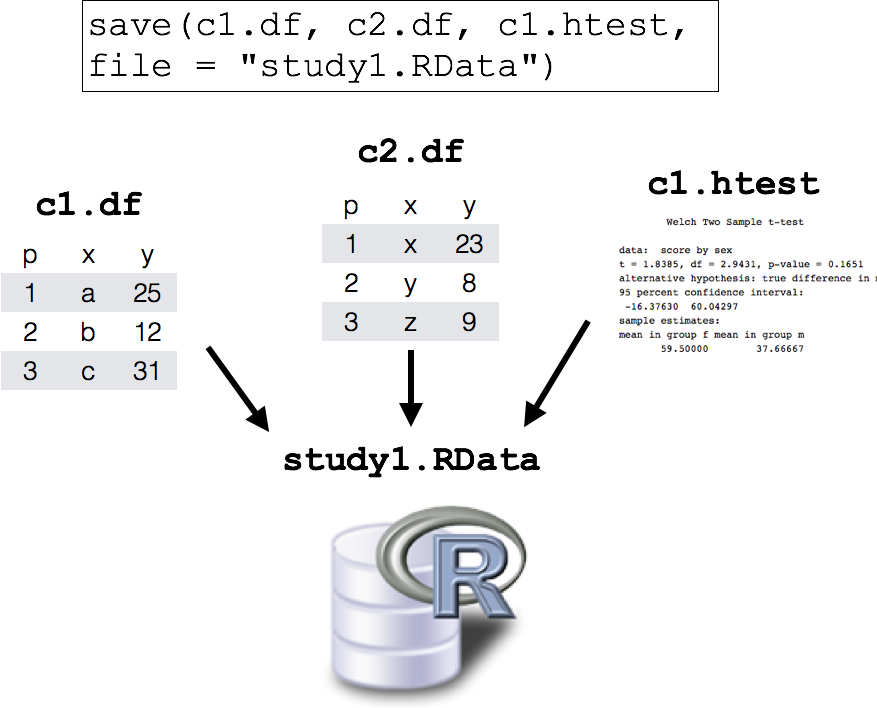
\includegraphics[width=0.75\linewidth]{images/rdata_example} 

}

\caption{Saving multiple objects into a single .RData file.}\label{fig:rdata}
\end{figure}

Now we will save all three objects that we imported into R, in an a file called \texttt{study1.RData} in the data folder of my current working directory. To do this, you can run the following

\begin{Shaded}
\begin{Highlighting}[]
\CommentTok{# Save three objects as a new .RData file}
\CommentTok{#   in the data folder of my current working directory}

\KeywordTok{save}\NormalTok{(scalfac, }
\NormalTok{     strn, }
\NormalTok{     subjdat,}
     \DataTypeTok{file =} \StringTok{"data/study1.RData"}\NormalTok{)}
\end{Highlighting}
\end{Shaded}

\begin{figure}

{\centering 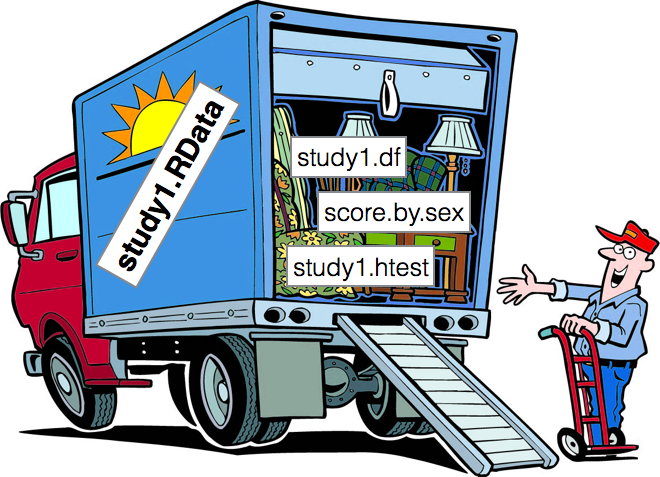
\includegraphics[width=0.75\linewidth]{images/rdatavan} 

}

\caption{Our new study1.RData file is like a van filled with our objects.}\label{fig:rdatavan}
\end{figure}

Once you do this, you should see the \texttt{study1.RData} file in the data folder of your working directory. This file now contains all of your objects that you can easily access later using the \texttt{load()} function (we'll go over this in a second\ldots).

\hypertarget{saving-entire-workspace}{%
\subsection{Saving entire workspace}\label{saving-entire-workspace}}

If you have many objects that you want to save, then using \texttt{save} can be tedious as you'd have to type the name of every object. To save \emph{all} the objects in your workspace as a .RData file, use the \texttt{save.image()} function. For example, to save my workspace in the \texttt{data} folder located in my working directory, I'd run the following:

\begin{Shaded}
\begin{Highlighting}[]
\CommentTok{# Save my workspace to complete_image.RData in th,e}
\CommentTok{#  data folder of my working directory}
\KeywordTok{save.image}\NormalTok{(}\DataTypeTok{file =} \StringTok{"data/projectimage.RData"}\NormalTok{)}
\end{Highlighting}
\end{Shaded}

\hypertarget{reading-in-the-saved-workspace}{%
\subsection{Reading in the saved workspace}\label{reading-in-the-saved-workspace}}

To load an \texttt{.RData} file, that is, to import all of the objects contained in the \texttt{.RData} file into your current workspace, use the \texttt{load()} function. For example, to load the three specific objects that I saved earlier (\texttt{study1.df}, \texttt{score.by.sex}, and \texttt{study1.htest}) in \texttt{study1.RData}, I'd run the following:

\begin{Shaded}
\begin{Highlighting}[]
\CommentTok{# Load objects in study1.RData into my workspace}
\KeywordTok{load}\NormalTok{(}\DataTypeTok{file =} \StringTok{"data/study1.RData"}\NormalTok{)}
\end{Highlighting}
\end{Shaded}

To load all of the objects in the workspace that I just saved to the data folder in my working directory in \texttt{projectimage.RData}, I'd run the following:

\begin{Shaded}
\begin{Highlighting}[]
\CommentTok{# Load objects in projectimage.RData into my workspace}
\KeywordTok{load}\NormalTok{(}\DataTypeTok{file =} \StringTok{"data/projectimage.RData"}\NormalTok{)}
\end{Highlighting}
\end{Shaded}

I hope you realize how awesome loading .RData files is. With R, you can store all of your objects, from dataframes to hypothesis tests, in a single \texttt{.RData} file. And then load them into any R session at any time using \texttt{load()}.

\hypertarget{clearing-the-workspace}{%
\section{Clearing the workspace}\label{clearing-the-workspace}}

To remove objects from your workspace, use the \texttt{rm()} function. Why would you want to remove objects? At some points in your analyses, you may find that your workspace is filled up with one or more objects that you don't need -- either because they're slowing down your computer, or because they're just distracting.

To remove specific objects, enter the objects as arguments to \texttt{rm()}. For example, to remove a huge dataframe called \texttt{scalfac}, I'd run the following;

\begin{Shaded}
\begin{Highlighting}[]
\CommentTok{# Remove scalfac from workspace}
\KeywordTok{rm}\NormalTok{(scalfac)}
\end{Highlighting}
\end{Shaded}

If you want to remove \emph{all} of the objects in your working directory, enter the argument \texttt{list\ =\ ls()}

\begin{Shaded}
\begin{Highlighting}[]
\CommentTok{# Remove ALL objects from workspace}
\KeywordTok{rm}\NormalTok{(}\DataTypeTok{list =} \KeywordTok{ls}\NormalTok{())}
\end{Highlighting}
\end{Shaded}

\textbf{Important!!!} Once you remove an object, you \textbf{cannot} get it back without running the code that originally generated the object! That is, you can't simply click `Undo' to get an object back. Thankfully, if your R code is complete and well-documented, you should easily be able to either re-create a lost object (e.g.; the results of a regression analysis), or re-load it from an external file.

\hypertarget{learning-check}{%
\section*{Learning check}\label{learning-check}}
\addcontentsline{toc}{section}{Learning check}

\begin{enumerate}
\def\labelenumi{\arabic{enumi}.}
\item
  Open up your \texttt{practice.Rmd}. Run the code chunks you created in sequential order.
\item
  Create a code chunk and open up the three files above into the R workspace.
\item
  Copy and Paste the three files \texttt{SubjectData.txt}, \texttt{scaleFact.txt}, \texttt{STRENGTH.xlsx}, from this books \texttt{data} folder, into your \texttt{se747/analysis/data} folder.
\item
  Open up your \texttt{practice.Rmd}. Run the code chunks you created in sequential order.
\item
  Create a code chunk and open up the three files above into the R workspace. Assign the data from \texttt{scaleFact.txt} to \texttt{scalfac}, \texttt{STRENGTH.xlsx} to \texttt{strn}, and \texttt{SubjectData.txt} to \texttt{subjdat}
\end{enumerate}

\hypertarget{part-data-manipulation-via-tidyverse}{%
\part{Data manipulation via tidyverse}\label{part-data-manipulation-via-tidyverse}}

\hypertarget{data-manipulation}{%
\chapter{Data manipulation}\label{data-manipulation}}

\hypertarget{download-and-load-libraries}{%
\section*{Download and load libraries}\label{download-and-load-libraries}}
\addcontentsline{toc}{section}{Download and load libraries}

\begin{Shaded}
\begin{Highlighting}[]
\ControlFlowTok{if}\NormalTok{ (}\OperatorTok{!}\KeywordTok{require}\NormalTok{(}\StringTok{"pacman"}\NormalTok{)) }\KeywordTok{install.packages}\NormalTok{(}\StringTok{"pacman"}\NormalTok{)}
\NormalTok{pacman}\OperatorTok{::}\KeywordTok{p_load}\NormalTok{(tidyverse, }\CommentTok{# All purpose wrangling for dataframes}
\NormalTok{               readr, }\CommentTok{# importing and writing data}
\NormalTok{               openxlsx, }\CommentTok{# writing excel documents}
\NormalTok{               purrr, }\CommentTok{# for piping %>%}
\NormalTok{               corrplot, }\CommentTok{# for correlation}
\NormalTok{               knitr,}
\NormalTok{               yarrr)}
\end{Highlighting}
\end{Shaded}

\hypertarget{import-data}{%
\section*{Import data}\label{import-data}}
\addcontentsline{toc}{section}{Import data}

Let's load the 3 files from \texttt{data} folder into the workspace again.

\begin{Shaded}
\begin{Highlighting}[]
\NormalTok{subjdat <-}\StringTok{  }\KeywordTok{read_delim}\NormalTok{ (}\DataTypeTok{file =} \StringTok{"data/SubjectData.txt"}\NormalTok{, }\CommentTok{# file name}
                        \DataTypeTok{delim =} \StringTok{"}\CharTok{\textbackslash{}t}\StringTok{"}\NormalTok{, }\CommentTok{# file separater}
                        \DataTypeTok{col_names =} \OtherTok{TRUE}\NormalTok{) }\CommentTok{# the first row of the data is a header row}

\NormalTok{scalfac <-}\StringTok{  }\KeywordTok{read_delim}\NormalTok{ (}\DataTypeTok{file =} \StringTok{"data/ScaleFact.txt"}\NormalTok{, }\CommentTok{# file name}
                        \DataTypeTok{delim =} \StringTok{"}\CharTok{\textbackslash{}t}\StringTok{"}\NormalTok{, }\CommentTok{# file separater}
                        \DataTypeTok{col_names =} \OtherTok{TRUE}\NormalTok{) }\CommentTok{# the first row of the data is a header row}

\NormalTok{strn <-}\StringTok{  }\KeywordTok{read.xlsx}\NormalTok{ (}\DataTypeTok{xlsxFile =} \StringTok{"data/STRENGTH.xlsx"}\NormalTok{)}
\end{Highlighting}
\end{Shaded}

\hypertarget{data-overview}{%
\section*{Data overview}\label{data-overview}}
\addcontentsline{toc}{section}{Data overview}

Design: This is a randomized controlled trial of two groups undergoing two strength training programs. Each subject was tested before and after training for their ankle and knee extensor strength variables.

Number of Subjects:32
Number of Groups: 2
Number of sides: 2
Number of repetitions: variable between 2 to 4

\hypertarget{peeking-at-the-data}{%
\section{Peeking at the Data}\label{peeking-at-the-data}}

Let's take a look at the first 6 (by default) rows of data:

\begin{Shaded}
\begin{Highlighting}[]
\KeywordTok{head}\NormalTok{(subjdat) }\CommentTok{#look at the top rows}
\end{Highlighting}
\end{Shaded}

\begin{verbatim}
## # A tibble: 6 x 17
##    SUBJ GROUP   AGE    WT    HT   BMI `RunExp ` RunFreq6wks RunFreq12mths
##   <dbl> <chr> <dbl> <dbl> <dbl> <dbl>     <dbl>       <dbl>         <dbl>
## 1     1 G        29  82.3  182   24.8        10           3             3
## 2     2 G        34  42.3  161   16.3         5           2             2
## 3     3 T        36  90.5  166   32.8         3           5             3
## 4     4 G        42  82.8  183   24.7        10           1             1
## 5     5 T        28  66.3  169   23.2         5           5             4
## 6     6 T        34  72.8  172.  24.5        16           6             6
## # ... with 8 more variables: RunDistWkly6wks <dbl>, RunDistWkly12mths <dbl>,
## #   LoadRunExp <chr>, RunLoad <dbl>, HxLoad <chr>, WtTrainFreq6wks <dbl>,
## #   WtTrainFreq12mths <dbl>, WtTrainStatus <chr>
\end{verbatim}

\begin{Shaded}
\begin{Highlighting}[]
\KeywordTok{tail}\NormalTok{ (subjdat) }\CommentTok{#look at the bottom rows}
\end{Highlighting}
\end{Shaded}

\begin{verbatim}
## # A tibble: 6 x 17
##    SUBJ GROUP   AGE    WT    HT   BMI `RunExp ` RunFreq6wks RunFreq12mths
##   <dbl> <chr> <dbl> <dbl> <dbl> <dbl>     <dbl>       <dbl>         <dbl>
## 1    27 T        20  57.5  168.  20.4        10           4             3
## 2    28 T        26  62.8  157.  25.6         2           1             3
## 3    29 T        18  83.4  183.  24.8         3           3             4
## 4    30 G        29  83.9  178.  26.4        15           4             2
## 5    31 G        32  67.9  177   21.7         5           1             2
## 6    32 G        19  47.7  167   17.1        10           3             1
## # ... with 8 more variables: RunDistWkly6wks <dbl>, RunDistWkly12mths <dbl>,
## #   LoadRunExp <chr>, RunLoad <dbl>, HxLoad <chr>, WtTrainFreq6wks <dbl>,
## #   WtTrainFreq12mths <dbl>, WtTrainStatus <chr>
\end{verbatim}

\hypertarget{checking-the-number-of-rows-and-columns-we-have-in-our-strength-data}{%
\section{Checking the number of rows and columns we have in our strength data}\label{checking-the-number-of-rows-and-columns-we-have-in-our-strength-data}}

I like to do this first, as it is the most basic check - does the number columns and rows conform to the number of variables you entered and the number of observations measured.

\begin{Shaded}
\begin{Highlighting}[]
\NormalTok{dimn <-}\StringTok{ }\KeywordTok{dim}\NormalTok{(strn)}

\CommentTok{# Print the number }
\KeywordTok{cat}\NormalTok{ (}\StringTok{"The number of rows is:"}\NormalTok{,  dimn[}\DecValTok{1}\NormalTok{], }\StringTok{"}\CharTok{\textbackslash{}n}\StringTok{"}\NormalTok{)}
\end{Highlighting}
\end{Shaded}

\begin{verbatim}
## The number of rows is: 992
\end{verbatim}

\begin{Shaded}
\begin{Highlighting}[]
\KeywordTok{cat}\NormalTok{ (}\StringTok{"The number of cols is:"}\NormalTok{,  dimn[}\DecValTok{2}\NormalTok{], }\StringTok{"}\CharTok{\textbackslash{}n}\StringTok{"}\NormalTok{)}
\end{Highlighting}
\end{Shaded}

\begin{verbatim}
## The number of cols is: 12
\end{verbatim}

\hypertarget{tidy-data}{%
\section{Tidy data}\label{tidy-data}}

You can represent the same underlying data in multiple ways. The example below shows the same data organised in four different ways. This dataset is \textbf{not the data you loaded}, but rather came with the \texttt{tidyverse\ package}. Each dataset shows the same values of four variables \emph{country}, \emph{year}, \emph{population}, and \emph{cases}, but each dataset organises the values in a different way.

\begin{Shaded}
\begin{Highlighting}[]
\NormalTok{table1}
\end{Highlighting}
\end{Shaded}

\begin{verbatim}
## # A tibble: 6 x 4
##   country      year  cases population
##   <chr>       <int>  <int>      <int>
## 1 Afghanistan  1999    745   19987071
## 2 Afghanistan  2000   2666   20595360
## 3 Brazil       1999  37737  172006362
## 4 Brazil       2000  80488  174504898
## 5 China        1999 212258 1272915272
## 6 China        2000 213766 1280428583
\end{verbatim}

\begin{Shaded}
\begin{Highlighting}[]
\NormalTok{table2}
\end{Highlighting}
\end{Shaded}

\begin{verbatim}
## # A tibble: 12 x 4
##    country      year type            count
##    <chr>       <int> <chr>           <int>
##  1 Afghanistan  1999 cases             745
##  2 Afghanistan  1999 population   19987071
##  3 Afghanistan  2000 cases            2666
##  4 Afghanistan  2000 population   20595360
##  5 Brazil       1999 cases           37737
##  6 Brazil       1999 population  172006362
##  7 Brazil       2000 cases           80488
##  8 Brazil       2000 population  174504898
##  9 China        1999 cases          212258
## 10 China        1999 population 1272915272
## 11 China        2000 cases          213766
## 12 China        2000 population 1280428583
\end{verbatim}

\begin{Shaded}
\begin{Highlighting}[]
\NormalTok{table3}
\end{Highlighting}
\end{Shaded}

\begin{verbatim}
## # A tibble: 6 x 3
##   country      year rate             
## * <chr>       <int> <chr>            
## 1 Afghanistan  1999 745/19987071     
## 2 Afghanistan  2000 2666/20595360    
## 3 Brazil       1999 37737/172006362  
## 4 Brazil       2000 80488/174504898  
## 5 China        1999 212258/1272915272
## 6 China        2000 213766/1280428583
\end{verbatim}

\begin{Shaded}
\begin{Highlighting}[]
\CommentTok{# Spread across two tables}
\NormalTok{table4a  }\CommentTok{# cases}
\end{Highlighting}
\end{Shaded}

\begin{verbatim}
## # A tibble: 3 x 3
##   country     `1999` `2000`
## * <chr>        <int>  <int>
## 1 Afghanistan    745   2666
## 2 Brazil       37737  80488
## 3 China       212258 213766
\end{verbatim}

\begin{Shaded}
\begin{Highlighting}[]
\NormalTok{table4b  }\CommentTok{# population}
\end{Highlighting}
\end{Shaded}

\begin{verbatim}
## # A tibble: 3 x 3
##   country         `1999`     `2000`
## * <chr>            <int>      <int>
## 1 Afghanistan   19987071   20595360
## 2 Brazil       172006362  174504898
## 3 China       1272915272 1280428583
\end{verbatim}

These are all representations of the same underlying data, but they are not equally easy to use. One dataset, the tidy dataset, will be much easier to work with.

There are three interrelated rules which make a dataset tidy:

\begin{enumerate}
\def\labelenumi{\arabic{enumi}.}
\tightlist
\item
  Each variable must have its own column.
\item
  Each observation must have its own row.
\item
  Each value must have its own cell.
\end{enumerate}

Figure \ref{fig:tidy-structure} shows the rules visually.

\begin{figure}
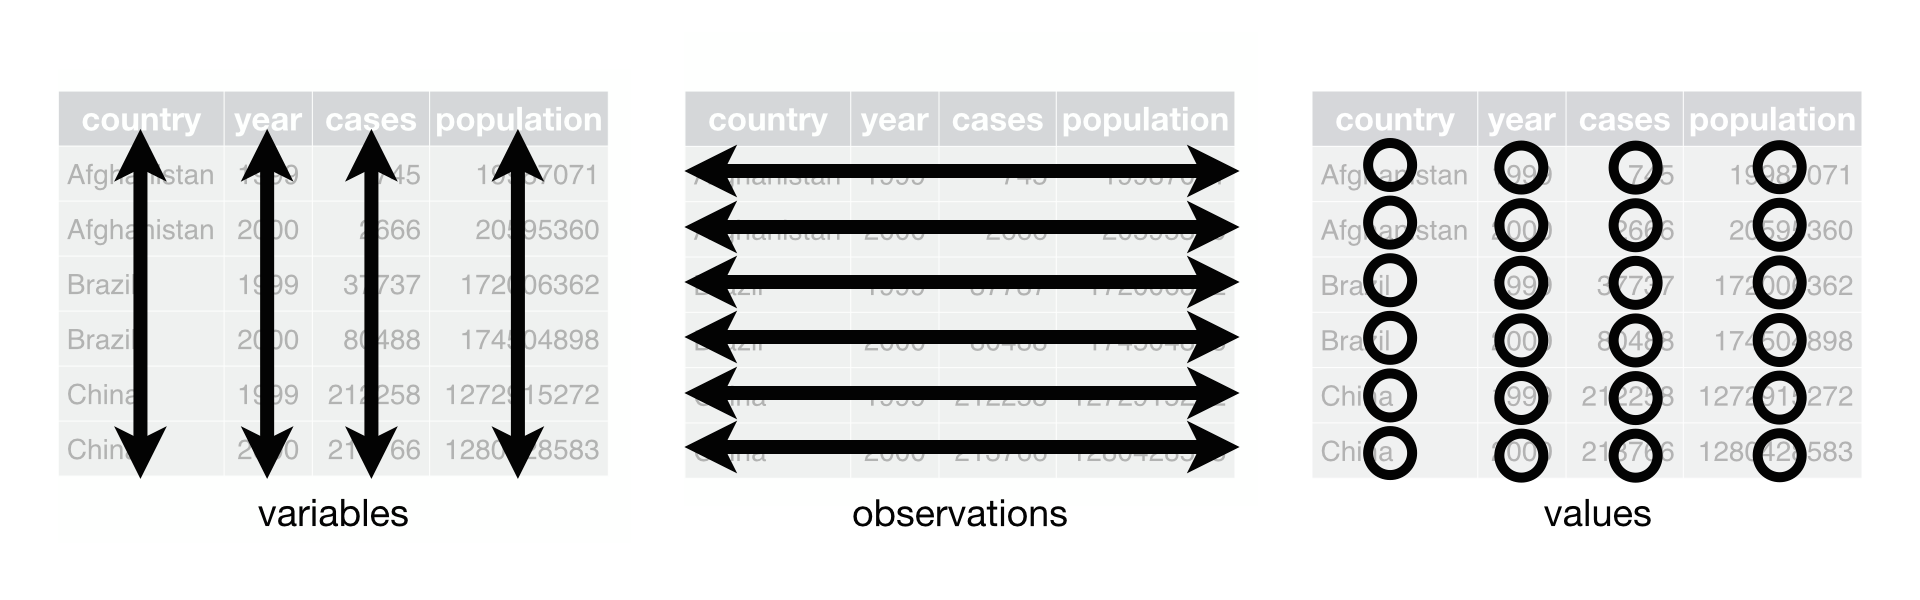
\includegraphics[width=1\linewidth]{images/tidy-1} \caption{Following three rules makes a dataset tidy: variables are in columns, observations are in rows, and values are in cells.}\label{fig:tidy-structure}
\end{figure}

These three rules are interrelated because it's impossible to only satisfy two of the three.

In this example, only \texttt{table1} is tidy. It's the only representation where each column is a variable.

Why ensure that your data is tidy? There are two main advantages:

\begin{enumerate}
\def\labelenumi{\arabic{enumi}.}
\item
  There's a general advantage to picking one consistent way of storing
  data. If you have a consistent data structure, it's easier to learn the
  tools that work with it because they have an underlying uniformity.
\item
  There's a specific advantage to placing variables in columns because
  it allows R's vectorised nature to shine. As you learned in
  \protect\hyperlink{mutate-funs}{mutate} and \protect\hyperlink{summary-funs}{summary functions}, most
  built-in R functions work with vectors of values. That makes transforming
  tidy data feel particularly natural.
\end{enumerate}

Let's have a look at our data \texttt{strn} which is in a tidy format. \textbf{the ``right'' way}

\begin{Shaded}
\begin{Highlighting}[]
\KeywordTok{head}\NormalTok{(strn) }\CommentTok{#look at the top rows}
\end{Highlighting}
\end{Shaded}

\begin{verbatim}
##   SUBJ GROUP TIME SIDE SET REP AEXTTORQ AEXTWORK AEXTPOW KEXTTORQ KEXTWORK
## 1    1     G  PRE    R   1   1       70       34      58      111      107
## 2    1     G  PRE    R   1   2       72       36      70      137      113
## 3    1     G  PRE    R   1   3       73       37      67      160      130
## 4    1     G  PRE    R   1   4       73       35      69      137      115
## 5    1     G  PRE    R   2   1       72       36      65      160      140
## 6    1     G  PRE    R   2   2       72       32      51      163      139
##   KEXTPOW
## 1      92
## 2     139
## 3     136
## 4     121
## 5     164
## 6     165
\end{verbatim}

\hypertarget{spreading-and-gathering}{%
\section{Spreading and gathering}\label{spreading-and-gathering}}

The principles of tidy data seem so obvious that you might wonder if you'll ever encounter a dataset that isn't tidy. Unfortunately, however, most data that you will encounter will be untidy. There are two main reasons:

\begin{enumerate}
\def\labelenumi{\arabic{enumi}.}
\item
  Most people aren't familiar with the principles of tidy data, and it's hard
  to derive them yourself unless you spend a \emph{lot} of time working with data.
\item
  Data is often organised to facilitate some use other than analysis. For
  example, data is often organised to make entry as easy as possible.
\end{enumerate}

This means for most real analyses, you'll need to do some tidying. The first step is always to figure out what the variables and observations are. Sometimes this is easy; other times you'll need to consult with the people who originally generated the data.
The second step is to resolve one of two common problems:

\begin{enumerate}
\def\labelenumi{\arabic{enumi}.}
\item
  One variable might be spread across multiple columns.
\item
  One observation might be scattered across multiple rows.
\end{enumerate}

Typically a dataset will only suffer from one of these problems; it'll only suffer from both if you're really unlucky! To fix these problems, you'll need the two most important functions in tidyr: \texttt{gather()} and \texttt{spread()}.

\hypertarget{spreading}{%
\subsection*{Spreading}\label{spreading}}
\addcontentsline{toc}{subsection}{Spreading}

Let's make it wide. This is how you probably entered your data.

\begin{Shaded}
\begin{Highlighting}[]
\NormalTok{wide <-}\StringTok{ }\NormalTok{strn }\OperatorTok\StringTok{ }\CommentTok{# original data}
\StringTok{  }\KeywordTok{unite}\NormalTok{ (}\StringTok{"time_side_set_rep"}\NormalTok{, }\CommentTok{# give the new variable a name}
\NormalTok{         TIME, SIDE, SET, REP, }\CommentTok{# merged different columns of data into one}
         \DataTypeTok{sep =} \StringTok{"_"}\NormalTok{) }\OperatorTok\StringTok{ }\CommentTok{# choose a separator. I like "_"}
\StringTok{  }\KeywordTok{select}\NormalTok{ (SUBJ, GROUP, time_side_set_rep, AEXTTORQ) }\OperatorTok\StringTok{ }\CommentTok{# choose columns which I want and discard the rest}
\StringTok{  }\KeywordTok{spread}\NormalTok{ (}\DataTypeTok{key =}\NormalTok{ time_side_set_rep, }\DataTypeTok{value =}\NormalTok{ AEXTTORQ) }\CommentTok{# spread it}

\KeywordTok{head}\NormalTok{ (wide)}
\end{Highlighting}
\end{Shaded}

\begin{verbatim}
##   SUBJ GROUP POST_L_1_1 POST_L_1_2 POST_L_1_3 POST_L_1_4 POST_L_2_1 POST_L_2_2
## 1    1     G         73         79         78         76         79         81
## 2    2     G         60         56         58         61         57         60
## 3    3     T         72         75         76         68         74         64
## 4    4     G         90         95         94         89        104        100
## 5    5     T        100         93         91         98        101        106
## 6    6     T        109        115        113        102        109        117
##   POST_L_2_3 POST_L_2_4 POST_R_1_1 POST_R_1_2 POST_R_1_3 POST_R_1_4 POST_R_2_1
## 1         78         79         74         76         77         80         86
## 2         64         64         60         66         64         68         58
## 3         84         74         94         92         93         94         88
## 4        105        111         93         92         92         92        108
## 5        104        104         92         94         92         89         93
## 6        118        118        108        111        105        120        127
##   POST_R_2_2 POST_R_2_3 POST_R_2_4 PRE_L_1_1 PRE_L_1_2 PRE_L_1_3 PRE_L_1_4
## 1         88         89         85        66        59        66        63
## 2         62         62         62        41        44        42        41
## 3         87         86         88        55        45        54        58
## 4        107        104        106        58        60        57        58
## 5         87         92         85        62        64        57        57
## 6        120        120        121        84        88        80        78
##   PRE_L_2_1 PRE_L_2_2 PRE_L_2_3 PRE_L_2_4 PRE_R_1_1 PRE_R_1_2 PRE_R_1_3
## 1        64        72        66        67    70.000    72.000   73.0000
## 2        42        41        40        33    52.000    54.000   60.0000
## 3        54        56        53        52    57.000    64.000   65.0000
## 4        58        59        61        65    58.000    50.000   65.0000
## 5        70        68        69        71    68.132    65.249   67.9594
## 6        85        79        82        86    76.000   100.000   89.0000
##   PRE_R_1_4 PRE_R_2_1 PRE_R_2_2 PRE_R_2_3 PRE_R_2_4
## 1   73.0000   72.0000   72.0000    67.000   72.0000
## 2   56.0000   47.0000   47.0000    50.000   54.0000
## 3   62.0000   76.0000   75.0000    86.000   82.0000
## 4   71.0000   75.0000   65.0000    71.000   75.0000
## 5   63.5177   60.1266   58.8245    63.419   58.0649
## 6   90.0000   88.0000   80.0000    86.000   88.0000
\end{verbatim}

\hypertarget{gathering}{%
\subsection*{Gathering}\label{gathering}}
\addcontentsline{toc}{subsection}{Gathering}

If your data is wide originally, make sure you have a very consistent labelling system. Then you can convert between formats easily.

Let's make it tall again. Converting messy data to tidy data. Why is it important to have a consistent naming terminology? It is a bad idea to use mathematical operators (e.g.~"*``,''-``,''") when naming, bad idea to have spaces when naming, and long names (e.g.``ankle\_kinematics\_sagittal\_plane'').

\begin{Shaded}
\begin{Highlighting}[]
\NormalTok{tall  <-}\StringTok{  }\NormalTok{wide }\OperatorTok
\StringTok{  }\KeywordTok{gather}\NormalTok{ (}\OperatorTok{-}\KeywordTok{c}\NormalTok{(}\DecValTok{1}\OperatorTok{:}\DecValTok{2}\NormalTok{), }\CommentTok{# I want to gather all columns except the first two columns}
          \DataTypeTok{key =}\NormalTok{ time_side_set_rep, }\CommentTok{# column name which contains the variable names}
          \DataTypeTok{value =}\NormalTok{ AEXTTORQ) }\OperatorTok\StringTok{ }\CommentTok{# column name containing the values}
\StringTok{  }\KeywordTok{separate}\NormalTok{ (time_side_set_rep, }\CommentTok{# split a long word in one column}
            \DataTypeTok{into =} \KeywordTok{c}\NormalTok{(}\StringTok{"TIME"}\NormalTok{, }\StringTok{"SIDE"}\NormalTok{, }\StringTok{"SET"}\NormalTok{, }\StringTok{"REP"}\NormalTok{), }\DataTypeTok{sep =} \StringTok{"_"}\NormalTok{) }\CommentTok{# give it column names}

\KeywordTok{head}\NormalTok{ (tall)}\CommentTok{# see how I recreate the original data?}
\end{Highlighting}
\end{Shaded}

\begin{verbatim}
##   SUBJ GROUP TIME SIDE SET REP AEXTTORQ
## 1    1     G POST    L   1   1       73
## 2    2     G POST    L   1   1       60
## 3    3     T POST    L   1   1       72
## 4    4     G POST    L   1   1       90
## 5    5     T POST    L   1   1      100
## 6    6     T POST    L   1   1      109
\end{verbatim}

\hypertarget{renaming-variables-and-values}{%
\section{Renaming variables and values}\label{renaming-variables-and-values}}

\hypertarget{rename-variable-names}{%
\subsection*{Rename variable names}\label{rename-variable-names}}
\addcontentsline{toc}{subsection}{Rename variable names}

I dislike excessively using capitals. It is alot of effort.

\begin{Shaded}
\begin{Highlighting}[]
\CommentTok{# Upper to lower caps}
\KeywordTok{colnames}\NormalTok{ (strn) <-}\StringTok{  }\KeywordTok{tolower}\NormalTok{(}\KeywordTok{colnames}\NormalTok{ (strn)) }\CommentTok{# captials to lower caps}

\CommentTok{# Manually create new names}
\NormalTok{strn <-}\StringTok{ }\NormalTok{strn }\OperatorTok
\StringTok{  }\KeywordTok{rename}\NormalTok{ (}\DataTypeTok{atorq =}\NormalTok{ aexttorq, }\CommentTok{# new name = old name}
          \DataTypeTok{awork =}\NormalTok{ aextwork,}
          \DataTypeTok{apow =}\NormalTok{ aextpow,}
          \DataTypeTok{ktorq =}\NormalTok{ kexttorq,}
          \DataTypeTok{kwork =}\NormalTok{ kextwork,}
          \DataTypeTok{kpow =}\NormalTok{ kextpow)}

\KeywordTok{head}\NormalTok{ (strn)}
\end{Highlighting}
\end{Shaded}

\begin{verbatim}
##   subj group time side set rep atorq awork apow ktorq kwork kpow
## 1    1     G  PRE    R   1   1    70    34   58   111   107   92
## 2    1     G  PRE    R   1   2    72    36   70   137   113  139
## 3    1     G  PRE    R   1   3    73    37   67   160   130  136
## 4    1     G  PRE    R   1   4    73    35   69   137   115  121
## 5    1     G  PRE    R   2   1    72    36   65   160   140  164
## 6    1     G  PRE    R   2   2    72    32   51   163   139  165
\end{verbatim}

\hypertarget{rename-values-in-variable-names}{%
\subsection*{Rename values in variable names}\label{rename-values-in-variable-names}}
\addcontentsline{toc}{subsection}{Rename values in variable names}

Let's us rename the values within the variable called GROUP. Instead of G, call it general; instead of T, call it target

\begin{Shaded}
\begin{Highlighting}[]
\NormalTok{strn <-}\StringTok{ }\NormalTok{strn }\OperatorTok
\StringTok{  }\KeywordTok{mutate}\NormalTok{ (}\DataTypeTok{group =} \KeywordTok{recode}\NormalTok{ (group, }\CommentTok{# the variable name}
                          \StringTok{"G"}\NormalTok{ =}\StringTok{ "general"}\NormalTok{, }\CommentTok{# old label = new label}
                          \StringTok{"T"}\NormalTok{ =}\StringTok{ "target"}\NormalTok{)) }\CommentTok{# old label = new label}

\KeywordTok{head}\NormalTok{ (strn)}
\end{Highlighting}
\end{Shaded}

\begin{verbatim}
##   subj   group time side set rep atorq awork apow ktorq kwork kpow
## 1    1 general  PRE    R   1   1    70    34   58   111   107   92
## 2    1 general  PRE    R   1   2    72    36   70   137   113  139
## 3    1 general  PRE    R   1   3    73    37   67   160   130  136
## 4    1 general  PRE    R   1   4    73    35   69   137   115  121
## 5    1 general  PRE    R   2   1    72    36   65   160   140  164
## 6    1 general  PRE    R   2   2    72    32   51   163   139  165
\end{verbatim}

\hypertarget{creating-factors}{%
\subsection*{Creating factors}\label{creating-factors}}
\addcontentsline{toc}{subsection}{Creating factors}

Since R can handle factor variables (see \texttt{?factor}), we can recode the levels to be more intuitive. Why do you need to convert categorical variables to factors? For now, let's accept it, for every statistical thing you do with categorical variables must be factors.

Make group, time, side, a factor

\begin{Shaded}
\begin{Highlighting}[]
\NormalTok{strn <-}\StringTok{  }\NormalTok{strn }\OperatorTok
\StringTok{  }\KeywordTok{mutate}\NormalTok{ (}\DataTypeTok{group =} \KeywordTok{factor}\NormalTok{ (group, }\DataTypeTok{levels =} \KeywordTok{c}\NormalTok{(}\StringTok{"general"}\NormalTok{, }\StringTok{"target"}\NormalTok{)), }\CommentTok{# levels = c(first, second)}
          \DataTypeTok{time =} \KeywordTok{factor}\NormalTok{ (time, }\DataTypeTok{levels =} \KeywordTok{c}\NormalTok{(}\StringTok{"PRE"}\NormalTok{, }\StringTok{"POST"}\NormalTok{)),}
          \DataTypeTok{side =} \KeywordTok{factor}\NormalTok{ (side, }\DataTypeTok{levels =} \KeywordTok{c}\NormalTok{(}\StringTok{"L"}\NormalTok{, }\StringTok{"R"}\NormalTok{)))}

\KeywordTok{head}\NormalTok{ (strn)}
\end{Highlighting}
\end{Shaded}

\begin{verbatim}
##   subj   group time side set rep atorq awork apow ktorq kwork kpow
## 1    1 general  PRE    R   1   1    70    34   58   111   107   92
## 2    1 general  PRE    R   1   2    72    36   70   137   113  139
## 3    1 general  PRE    R   1   3    73    37   67   160   130  136
## 4    1 general  PRE    R   1   4    73    35   69   137   115  121
## 5    1 general  PRE    R   2   1    72    36   65   160   140  164
## 6    1 general  PRE    R   2   2    72    32   51   163   139  165
\end{verbatim}

\hypertarget{making-a-new-variable}{%
\section{Making a new variable}\label{making-a-new-variable}}

I want to:

\begin{enumerate}
\def\labelenumi{\arabic{enumi}.}
\tightlist
\item
  add ankle torque and knee torque to create a new variable called total torque
\item
  subtract their torques to create a variable called dtorq
\end{enumerate}

\begin{Shaded}
\begin{Highlighting}[]
\NormalTok{strn <-}\StringTok{  }\NormalTok{strn }\OperatorTok
\StringTok{  }\KeywordTok{mutate}\NormalTok{ (}\DataTypeTok{ttorq =}\NormalTok{ atorq }\OperatorTok{+}\StringTok{ }\NormalTok{ktorq, }\CommentTok{# this will add a new variable called ttorq}
          \DataTypeTok{dtorq =}\NormalTok{ atorq }\OperatorTok{-}\StringTok{ }\NormalTok{ktorq) }\CommentTok{# this will add a new variable called dtorq}
\KeywordTok{head}\NormalTok{ (strn)}
\end{Highlighting}
\end{Shaded}

\begin{verbatim}
##   subj   group time side set rep atorq awork apow ktorq kwork kpow ttorq dtorq
## 1    1 general  PRE    R   1   1    70    34   58   111   107   92   181   -41
## 2    1 general  PRE    R   1   2    72    36   70   137   113  139   209   -65
## 3    1 general  PRE    R   1   3    73    37   67   160   130  136   233   -87
## 4    1 general  PRE    R   1   4    73    35   69   137   115  121   210   -64
## 5    1 general  PRE    R   2   1    72    36   65   160   140  164   232   -88
## 6    1 general  PRE    R   2   2    72    32   51   163   139  165   235   -91
\end{verbatim}

You are only interested in the change scores of each subject's average strength

\begin{Shaded}
\begin{Highlighting}[]
\NormalTok{strn_change <-}\StringTok{  }\NormalTok{strn }\OperatorTok\StringTok{ }\CommentTok{# original data}
\StringTok{  }\KeywordTok{group_by}\NormalTok{(subj, group, time) }\OperatorTok\StringTok{ }\CommentTok{# calculate an outcome per group}
\StringTok{  }\KeywordTok{summarize}\NormalTok{ (}\DataTypeTok{atorq =} \KeywordTok{mean}\NormalTok{ (atorq)) }\OperatorTok\StringTok{ }\CommentTok{# in this case you want to calculate average}
\StringTok{  }\KeywordTok{spread}\NormalTok{ (}\DataTypeTok{key =}\NormalTok{ time, }\DataTypeTok{value =}\NormalTok{ atorq) }\OperatorTok\StringTok{ }\CommentTok{# spread it}
\StringTok{  }\KeywordTok{mutate}\NormalTok{ (}\DataTypeTok{atorq_diff =}\NormalTok{ POST}\OperatorTok{-}\NormalTok{PRE)  }\OperatorTok\StringTok{ }\CommentTok{# find the difference}
\StringTok{  }\KeywordTok{ungroup}\NormalTok{ ()}
\end{Highlighting}
\end{Shaded}

\begin{verbatim}
## `summarise()` regrouping output by 'subj', 'group' (override with `.groups` argument)
\end{verbatim}

\begin{Shaded}
\begin{Highlighting}[]
\KeywordTok{head}\NormalTok{ (strn)}
\end{Highlighting}
\end{Shaded}

\begin{verbatim}
##   subj   group time side set rep atorq awork apow ktorq kwork kpow ttorq dtorq
## 1    1 general  PRE    R   1   1    70    34   58   111   107   92   181   -41
## 2    1 general  PRE    R   1   2    72    36   70   137   113  139   209   -65
## 3    1 general  PRE    R   1   3    73    37   67   160   130  136   233   -87
## 4    1 general  PRE    R   1   4    73    35   69   137   115  121   210   -64
## 5    1 general  PRE    R   2   1    72    36   65   160   140  164   232   -88
## 6    1 general  PRE    R   2   2    72    32   51   163   139  165   235   -91
\end{verbatim}

\hypertarget{transforming-a-variable}{%
\section{Transforming a variable}\label{transforming-a-variable}}

The subject's mass is stored in another file called \texttt{subjdat}. we need to merge two documents making sure each row is joined correctly.

\begin{Shaded}
\begin{Highlighting}[]
\CommentTok{# convert names to lower cases}
\KeywordTok{colnames}\NormalTok{ (subjdat)  <-}\StringTok{  }\KeywordTok{tolower}\NormalTok{ (}\KeywordTok{colnames}\NormalTok{ (subjdat))}

\CommentTok{# create another object, keeping only two variables of }
\NormalTok{subj_mass <-}\StringTok{  }\KeywordTok{select}\NormalTok{ (subjdat, }\CommentTok{# original dataframe}
\NormalTok{                      subj, wt) }\CommentTok{# two variables}

\CommentTok{# }
\NormalTok{strn_scal <-}\StringTok{  }\NormalTok{subj_mass }\OperatorTok
\StringTok{  }\KeywordTok{inner_join}\NormalTok{(strn, }\DataTypeTok{by =} \StringTok{"subj"}\NormalTok{) }\OperatorTok\StringTok{ }\CommentTok{# combine two dataframes, ensuring each rows are combined exactly}
\StringTok{  }\KeywordTok{mutate}\NormalTok{ (}\DataTypeTok{ttorq_s =}\NormalTok{ ttorq}\OperatorTok{/}\NormalTok{wt, }\CommentTok{# divide total torque by weight}
          \DataTypeTok{dtorq_s =}\NormalTok{ dtorq}\OperatorTok{/}\NormalTok{wt) }\CommentTok{# divide difference torque by weight}

\KeywordTok{head}\NormalTok{ (strn_scal)}
\end{Highlighting}
\end{Shaded}

\begin{verbatim}
## # A tibble: 6 x 17
##    subj    wt group  time  side    set   rep atorq awork  apow ktorq kwork  kpow
##   <dbl> <dbl> <fct>  <fct> <fct> <dbl> <dbl> <dbl> <dbl> <dbl> <dbl> <dbl> <dbl>
## 1     1  82.3 gener~ PRE   R         1     1    70    34    58   111   107    92
## 2     1  82.3 gener~ PRE   R         1     2    72    36    70   137   113   139
## 3     1  82.3 gener~ PRE   R         1     3    73    37    67   160   130   136
## 4     1  82.3 gener~ PRE   R         1     4    73    35    69   137   115   121
## 5     1  82.3 gener~ PRE   R         2     1    72    36    65   160   140   164
## 6     1  82.3 gener~ PRE   R         2     2    72    32    51   163   139   165
## # ... with 4 more variables: ttorq <dbl>, dtorq <dbl>, ttorq_s <dbl>,
## #   dtorq_s <dbl>
\end{verbatim}

\hypertarget{filtering}{%
\section{Filtering}\label{filtering}}

Filtering is removing rows you do not want and keeping rows you want based on some condition(s).

\hypertarget{keep-rows-based-on-category-you-wish-to-keep}{%
\subsection{Keep rows based on category you wish to keep}\label{keep-rows-based-on-category-you-wish-to-keep}}

You are only interested in keeping pre strength variables

\begin{Shaded}
\begin{Highlighting}[]
\NormalTok{strn_pre <-}\StringTok{  }\NormalTok{strn }\OperatorTok
\StringTok{      }\KeywordTok{filter}\NormalTok{ (time }\OperatorTok{==}\StringTok{ "PRE"}\NormalTok{)}

\KeywordTok{head}\NormalTok{ (strn_pre)}
\end{Highlighting}
\end{Shaded}

\begin{verbatim}
##   subj   group time side set rep atorq awork apow ktorq kwork kpow ttorq dtorq
## 1    1 general  PRE    R   1   1    70    34   58   111   107   92   181   -41
## 2    1 general  PRE    R   1   2    72    36   70   137   113  139   209   -65
## 3    1 general  PRE    R   1   3    73    37   67   160   130  136   233   -87
## 4    1 general  PRE    R   1   4    73    35   69   137   115  121   210   -64
## 5    1 general  PRE    R   2   1    72    36   65   160   140  164   232   -88
## 6    1 general  PRE    R   2   2    72    32   51   163   139  165   235   -91
\end{verbatim}

\hypertarget{include-rows-based-on-a-numerical-range}{%
\subsection{Include rows based on a numerical range}\label{include-rows-based-on-a-numerical-range}}

Keep ankle torque values less than 100 in magnitude and knee torque more than 150

\begin{Shaded}
\begin{Highlighting}[]
\NormalTok{strn_filt <-}\StringTok{  }\NormalTok{strn }\OperatorTok
\StringTok{      }\KeywordTok{filter}\NormalTok{ (atorq }\OperatorTok{<}\StringTok{ }\DecValTok{100} \OperatorTok{&}\StringTok{ }\NormalTok{ktorq }\OperatorTok{>}\StringTok{ }\DecValTok{150}\NormalTok{)}

\KeywordTok{head}\NormalTok{ (strn_filt)}
\end{Highlighting}
\end{Shaded}

\begin{verbatim}
##   subj   group time side set rep atorq awork apow ktorq kwork kpow ttorq dtorq
## 1    1 general  PRE    R   1   3    73    37   67   160   130  136   233   -87
## 2    1 general  PRE    R   2   1    72    36   65   160   140  164   232   -88
## 3    1 general  PRE    R   2   2    72    32   51   163   139  165   235   -91
## 4    1 general  PRE    R   2   3    67    34   63   157   133  155   224   -90
## 5    1 general  PRE    R   2   4    72    36   66   165   145  158   237   -93
## 6    1 general  PRE    L   2   1    64    33   63   170   168  165   234  -106
\end{verbatim}

\hypertarget{exclude-rows-variables-based-on-a-numerical-range}{%
\subsection{Exclude rows variables based on a numerical range}\label{exclude-rows-variables-based-on-a-numerical-range}}

Exclude ankle torque values less than 100

\begin{Shaded}
\begin{Highlighting}[]
\CommentTok{# notice the !. It is equivalent to saying "not". Not less than 100 in this instance}

\NormalTok{strn_filt <-}\StringTok{  }\NormalTok{strn }\OperatorTok
\StringTok{      }\KeywordTok{filter}\NormalTok{ (}\OperatorTok{!}\NormalTok{atorq }\OperatorTok{<}\StringTok{ }\DecValTok{100}\NormalTok{) }

\KeywordTok{head}\NormalTok{ (strn_filt)}
\end{Highlighting}
\end{Shaded}

\begin{verbatim}
##   subj   group time side set rep atorq awork apow ktorq kwork kpow ttorq dtorq
## 1    4 general POST    R   2   1   108    50   76   182   194  177   290   -74
## 2    4 general POST    R   2   2   107    49   79   179   182  185   286   -72
## 3    4 general POST    R   2   3   104    44   74   169   180  175   273   -65
## 4    4 general POST    R   2   4   106    49   86   176   185  173   282   -70
## 5    4 general POST    L   2   1   104    50   95   138   166  141   242   -34
## 6    4 general POST    L   2   2   100    48   98   141   158  145   241   -41
\end{verbatim}

\hypertarget{selecting}{%
\section{Selecting}\label{selecting}}

Selecting removing columns you do not want and keeping columns you want

You are only interested in keeping columns \texttt{subj}, \texttt{group} in dataframe \texttt{strn}

\begin{Shaded}
\begin{Highlighting}[]
\NormalTok{strn.subset <-}\StringTok{  }\NormalTok{strn }\OperatorTok
\StringTok{      }\KeywordTok{select}\NormalTok{ (subj, group)}

\KeywordTok{head}\NormalTok{ (strn.subset)}
\end{Highlighting}
\end{Shaded}

\begin{verbatim}
##   subj   group
## 1    1 general
## 2    1 general
## 3    1 general
## 4    1 general
## 5    1 general
## 6    1 general
\end{verbatim}

\hypertarget{check-for-missing-na-values}{%
\section{Check for missing NA values}\label{check-for-missing-na-values}}

\hypertarget{check-if-there-is-any-missing}{%
\subsection{Check if there is any missing}\label{check-if-there-is-any-missing}}

\begin{Shaded}
\begin{Highlighting}[]
\NormalTok{na_count <-}\StringTok{  }\KeywordTok{sum}\NormalTok{ (}\KeywordTok{is.na}\NormalTok{ (strn))}

\KeywordTok{cat}\NormalTok{ (}\StringTok{"The number of missing values ="}\NormalTok{, na_count)}
\end{Highlighting}
\end{Shaded}

\begin{verbatim}
## The number of missing values = 0
\end{verbatim}

For the sick of practice, let me create a dataset with NA in each. You do not have to know this.

\begin{Shaded}
\begin{Highlighting}[]
\NormalTok{strn.miss <-}\StringTok{ }\NormalTok{strn}

\NormalTok{strn.miss[,}\KeywordTok{c}\NormalTok{(}\DecValTok{7}\OperatorTok{:}\DecValTok{14}\NormalTok{)] <-}\StringTok{  }\KeywordTok{map_df}\NormalTok{(strn.miss [,}\KeywordTok{c}\NormalTok{(}\DecValTok{7}\OperatorTok{:}\DecValTok{14}\NormalTok{)],}
                               \ControlFlowTok{function}\NormalTok{(x) \{x[}\KeywordTok{sample}\NormalTok{(}\KeywordTok{c}\NormalTok{(}\OtherTok{TRUE}\NormalTok{, }\OtherTok{NA}\NormalTok{), }
                                                     \DataTypeTok{prob =} \KeywordTok{c}\NormalTok{(}\FloatTok{0.9}\NormalTok{, }\FloatTok{0.1}\NormalTok{), }
                                                     \DataTypeTok{size =} \KeywordTok{length}\NormalTok{(x),}
                                                     \DataTypeTok{replace =} \OtherTok{TRUE}\NormalTok{)]\})}

\NormalTok{strn.miss [}\DecValTok{100}\NormalTok{,}\KeywordTok{c}\NormalTok{(}\DecValTok{7}\OperatorTok{:}\DecValTok{14}\NormalTok{)] =}\StringTok{ }\OtherTok{NA}

\NormalTok{na_count =}\StringTok{ }\KeywordTok{sum}\NormalTok{ (}\KeywordTok{is.na}\NormalTok{ (strn.miss))}

\KeywordTok{cat}\NormalTok{ (}\StringTok{"The number of missing values is now ="}\NormalTok{, na_count)}
\end{Highlighting}
\end{Shaded}

\begin{verbatim}
## The number of missing values is now = 854
\end{verbatim}

\hypertarget{find-the-number-of-missing-values-per-column}{%
\subsection{Find the number of missing values per column}\label{find-the-number-of-missing-values-per-column}}

\begin{Shaded}
\begin{Highlighting}[]
\NormalTok{na_count <-}\StringTok{  }\NormalTok{strn.miss }\OperatorTok
\StringTok{  }\KeywordTok{select}\NormalTok{(}\KeywordTok{everything}\NormalTok{()) }\OperatorTok\StringTok{  }\CommentTok{# replace to your needs}
\StringTok{  }\KeywordTok{summarise_all}\NormalTok{(}\KeywordTok{funs}\NormalTok{(}\KeywordTok{sum}\NormalTok{(}\KeywordTok{is.na}\NormalTok{(.))))}
\end{Highlighting}
\end{Shaded}

\begin{verbatim}
## Warning: `funs()` is deprecated as of dplyr 0.8.0.
## Please use a list of either functions or lambdas: 
## 
##   # Simple named list: 
##   list(mean = mean, median = median)
## 
##   # Auto named with `tibble::lst()`: 
##   tibble::lst(mean, median)
## 
##   # Using lambdas
##   list(~ mean(., trim = .2), ~ median(., na.rm = TRUE))
## This warning is displayed once every 8 hours.
## Call `lifecycle::last_warnings()` to see where this warning was generated.
\end{verbatim}

\begin{Shaded}
\begin{Highlighting}[]
\KeywordTok{kable}\NormalTok{ (na_count, }\DataTypeTok{caption =} \StringTok{"Number of missing per col"}\NormalTok{) }
\end{Highlighting}
\end{Shaded}

\begin{table}

\caption{\label{tab:unnamed-chunk-18}Number of missing per col}
\centering
\begin{tabular}[t]{r|r|r|r|r|r|r|r|r|r|r|r|r|r}
\hline
subj & group & time & side & set & rep & atorq & awork & apow & ktorq & kwork & kpow & ttorq & dtorq\\
\hline
0 & 0 & 0 & 0 & 0 & 0 & 103 & 108 & 92 & 102 & 125 & 100 & 111 & 113\\
\hline
\end{tabular}
\end{table}

\hypertarget{keep-rows-with-100-no-na-across-any-columns}{%
\subsection{Keep rows with 100\% no NA across any columns}\label{keep-rows-with-100-no-na-across-any-columns}}

\begin{Shaded}
\begin{Highlighting}[]
\NormalTok{strn_compl <-}\StringTok{  }\NormalTok{strn.miss }\OperatorTok
\StringTok{  }\KeywordTok{na.omit}\NormalTok{ ()}
\end{Highlighting}
\end{Shaded}

\hypertarget{keep-rows-with-100-no-na-across-the-columns-you-want}{%
\subsection{Keep rows with 100\% no NA across the columns you want}\label{keep-rows-with-100-no-na-across-the-columns-you-want}}

\begin{Shaded}
\begin{Highlighting}[]
\NormalTok{col2filt =}\StringTok{ }\KeywordTok{c}\NormalTok{(}\StringTok{"atorq"}\NormalTok{, }\StringTok{"ktorq"}\NormalTok{) }\CommentTok{# add as many variables you want}

\NormalTok{strn_compl <-}\StringTok{  }\NormalTok{strn.miss }\OperatorTok
\StringTok{  }\KeywordTok{filter_at}\NormalTok{(}\KeywordTok{vars}\NormalTok{(col2filt), }\KeywordTok{all_vars}\NormalTok{(}\KeywordTok{complete.cases}\NormalTok{(.)))}
\end{Highlighting}
\end{Shaded}

\begin{verbatim}
## Note: Using an external vector in selections is ambiguous.
## i Use `all_of(col2filt)` instead of `col2filt` to silence this message.
## i See <https://tidyselect.r-lib.org/reference/faq-external-vector.html>.
## This message is displayed once per session.
\end{verbatim}

\begin{Shaded}
\begin{Highlighting}[]
\KeywordTok{head}\NormalTok{ (strn_compl)}
\end{Highlighting}
\end{Shaded}

\begin{verbatim}
##   subj   group time side set rep atorq awork apow ktorq kwork kpow ttorq dtorq
## 1    1 general  PRE    R   1   1    70    34   58   111    NA   NA   181   -41
## 2    1 general  PRE    R   1   3    73    NA   67   160   130  136   233   -87
## 3    1 general  PRE    R   1   4    73    35   69   137   115  121   210   -64
## 4    1 general  PRE    R   2   1    72    NA   65   160   140  164   232   -88
## 5    1 general  PRE    R   2   2    72    NA   51   163   139  165   235   -91
## 6    1 general  PRE    R   2   3    67    34   63   157   133  155   224   -90
\end{verbatim}

\hypertarget{keep-rows-with-na-across-columns-you-want.}{%
\subsection{\texorpdfstring{Keep rows \textbf{with} NA across columns you want.}{Keep rows with NA across columns you want.}}\label{keep-rows-with-na-across-columns-you-want.}}

Keeping NA is useful if you want to inspect if the missing-ness is due to data entry errors, etc\ldots{}

\begin{Shaded}
\begin{Highlighting}[]
\NormalTok{col2filt =}\StringTok{ }\KeywordTok{c}\NormalTok{(}\StringTok{"atorq"}\NormalTok{, }\StringTok{"ktorq"}\NormalTok{) }\CommentTok{# add as many variables you want}

\NormalTok{strn_miss <-}\StringTok{  }\NormalTok{strn.miss }\OperatorTok
\StringTok{  }\KeywordTok{filter_at}\NormalTok{(}\KeywordTok{vars}\NormalTok{(col2filt), }\KeywordTok{all_vars}\NormalTok{(}\OperatorTok{!}\KeywordTok{complete.cases}\NormalTok{(.))) }

\KeywordTok{head}\NormalTok{ (strn_miss)}
\end{Highlighting}
\end{Shaded}

\begin{verbatim}
##   subj   group time side set rep atorq awork apow ktorq kwork kpow ttorq dtorq
## 1    1 general POST    L   2   3    NA    41   NA    NA   164   NA   224   -68
## 2    4 general  PRE    R   1   4    NA    NA   NA    NA    NA   NA    NA    NA
## 3    7 general  PRE    R   2   4    NA    36   75    NA   120  129   201    NA
## 4   17 general POST    L   2   1    NA    36   71    NA    91   86   162   -18
## 5   26 general POST    L   2   1    NA    44   91    NA   126  134    NA   -45
## 6   27  target POST    L   2   1    NA    40   76    NA    NA  153   208   -50
\end{verbatim}

\hypertarget{learning-check}{%
\section*{Learning check}\label{learning-check}}
\addcontentsline{toc}{section}{Learning check}

\begin{enumerate}
\def\labelenumi{\arabic{enumi}.}
\item
  Open up your \texttt{practice.Rmd}. Run the code chunks you created in sequential order.
\item
  Create a code chunk and open up the three files above into the R workspace. Subsequently, any task should automatically be associated with creating a new code chunk. If unsure, have more chunks.
\item
  Make all column header names to lowercases.
\item
  Remove \texttt{aexttorq} values that are below 75, and assign this new data to an object called \texttt{strn.sub}. How many rows are left in the new dataframe.
\end{enumerate}

\hypertarget{general-statistics}{%
\chapter{General statistics}\label{general-statistics}}

\hypertarget{download-and-load-libraries}{%
\section*{Download and load libraries}\label{download-and-load-libraries}}
\addcontentsline{toc}{section}{Download and load libraries}

\begin{Shaded}
\begin{Highlighting}[]
\ControlFlowTok{if}\NormalTok{ (}\OperatorTok{!}\KeywordTok{require}\NormalTok{(}\StringTok{"pacman"}\NormalTok{)) }\KeywordTok{install.packages}\NormalTok{(}\StringTok{"pacman"}\NormalTok{)}
\NormalTok{pacman}\OperatorTok{::}\KeywordTok{p_load}\NormalTok{(tidyverse, }\CommentTok{# All purpose wrangling for dataframes}
\NormalTok{               readr, }\CommentTok{# importing and writing data}
\NormalTok{               openxlsx, }\CommentTok{# writing excel documents}
\NormalTok{               purrr, }\CommentTok{# for piping %>%}
\NormalTok{               corrplot, }\CommentTok{# for correlation}
\NormalTok{               knitr,}
\NormalTok{               yarrr)}
\end{Highlighting}
\end{Shaded}

\hypertarget{import-data}{%
\section*{Import data}\label{import-data}}
\addcontentsline{toc}{section}{Import data}

Let's load the 3 files from \texttt{data} folder into the workspace again.

\begin{Shaded}
\begin{Highlighting}[]
\NormalTok{subjdat <-}\StringTok{  }\KeywordTok{read_delim}\NormalTok{ (}\DataTypeTok{file =} \StringTok{"data/SubjectData.txt"}\NormalTok{, }\CommentTok{# file name}
                        \DataTypeTok{delim =} \StringTok{"}\CharTok{\textbackslash{}t}\StringTok{"}\NormalTok{, }\CommentTok{# file separater}
                        \DataTypeTok{col_names =} \OtherTok{TRUE}\NormalTok{) }\CommentTok{# the first row of the data is a header row}

\NormalTok{scalfac <-}\StringTok{  }\KeywordTok{read_delim}\NormalTok{ (}\DataTypeTok{file =} \StringTok{"data/ScaleFact.txt"}\NormalTok{, }\CommentTok{# file name}
                        \DataTypeTok{delim =} \StringTok{"}\CharTok{\textbackslash{}t}\StringTok{"}\NormalTok{, }\CommentTok{# file separater}
                        \DataTypeTok{col_names =} \OtherTok{TRUE}\NormalTok{) }\CommentTok{# the first row of the data is a header row}

\NormalTok{strn <-}\StringTok{  }\KeywordTok{read.xlsx}\NormalTok{ (}\DataTypeTok{xlsxFile =} \StringTok{"data/STRENGTH.xlsx"}\NormalTok{)}
\end{Highlighting}
\end{Shaded}

\hypertarget{rename-column-names}{%
\section*{Rename column names}\label{rename-column-names}}
\addcontentsline{toc}{section}{Rename column names}

\begin{Shaded}
\begin{Highlighting}[]
\CommentTok{# Method 1:}
\KeywordTok{colnames}\NormalTok{ (strn) <-}\StringTok{  }\KeywordTok{tolower}\NormalTok{(}\KeywordTok{colnames}\NormalTok{ (strn)) }\CommentTok{# captials to lower caps}

\CommentTok{# Method 2: Define new names}
\NormalTok{newnames <-}\StringTok{ }\KeywordTok{c}\NormalTok{(}\StringTok{"atorq"}\NormalTok{, }\StringTok{"awork"}\NormalTok{, }\StringTok{"apow"}\NormalTok{, }\StringTok{"ktorq"}\NormalTok{, }\StringTok{"kwork"}\NormalTok{, }\StringTok{"kpow"}\NormalTok{)}
\CommentTok{# [7:12] tells the system the column numbers you want to replace. In this instance it is columns 7 to 12}
\KeywordTok{colnames}\NormalTok{ (strn)[}\DecValTok{7}\OperatorTok{:}\DecValTok{12}\NormalTok{] =}\StringTok{ }\NormalTok{newnames}
\end{Highlighting}
\end{Shaded}

\hypertarget{summarizing-your-data}{%
\section{Summarizing your data}\label{summarizing-your-data}}

The Solution exhibits the summary of a vector. The \texttt{1st\ Qu.} and \texttt{3rd\ Qu.} are the first and third quartile, respectively. Having both the median and mean is useful because you can
quickly detect skew.

\begin{Shaded}
\begin{Highlighting}[]
\CommentTok{# Quick way}
\KeywordTok{summary}\NormalTok{ (strn)}
\end{Highlighting}
\end{Shaded}

\begin{verbatim}
##       subj          group               time               side          
##  Min.   : 1.00   Length:992         Length:992         Length:992        
##  1st Qu.: 8.00   Class :character   Class :character   Class :character  
##  Median :17.00   Mode  :character   Mode  :character   Mode  :character  
##  Mean   :16.61                                                           
##  3rd Qu.:25.00                                                           
##  Max.   :32.00                                                           
##       set           rep           atorq            awork            apow       
##  Min.   :1.0   Min.   :1.00   Min.   : 33.00   Min.   :17.00   Min.   : 18.00  
##  1st Qu.:1.0   1st Qu.:1.75   1st Qu.: 67.00   1st Qu.:32.00   1st Qu.: 60.51  
##  Median :1.5   Median :2.50   Median : 82.00   Median :39.00   Median : 74.50  
##  Mean   :1.5   Mean   :2.50   Mean   : 83.94   Mean   :40.03   Mean   : 76.01  
##  3rd Qu.:2.0   3rd Qu.:3.25   3rd Qu.: 99.00   3rd Qu.:47.00   3rd Qu.: 90.00  
##  Max.   :2.0   Max.   :4.00   Max.   :145.00   Max.   :72.00   Max.   :151.00  
##      ktorq           kwork            kpow      
##  Min.   : 75.0   Min.   : 78.0   Min.   : 24.0  
##  1st Qu.:120.8   1st Qu.:124.0   1st Qu.:106.0  
##  Median :146.0   Median :145.0   Median :134.0  
##  Mean   :150.2   Mean   :151.8   Mean   :135.8  
##  3rd Qu.:175.0   3rd Qu.:172.0   3rd Qu.:165.0  
##  Max.   :322.0   Max.   :324.0   Max.   :328.0
\end{verbatim}

\begin{Shaded}
\begin{Highlighting}[]
\CommentTok{# Tidy way}

\NormalTok{strn }\OperatorTok
\StringTok{  }\KeywordTok{summarize}\NormalTok{ (}\DataTypeTok{Mean =} \KeywordTok{mean}\NormalTok{ (atorq, }\DataTypeTok{na.rm =}\NormalTok{ T),}
             \DataTypeTok{Median =} \KeywordTok{median}\NormalTok{ (atorq, }\DataTypeTok{na.rm =}\NormalTok{ T),}
             \DataTypeTok{Max =} \KeywordTok{max}\NormalTok{ (atorq, }\DataTypeTok{na.rm =}\NormalTok{ T),}
             \DataTypeTok{Min =} \KeywordTok{min}\NormalTok{ (atorq, }\DataTypeTok{na.rm =}\NormalTok{ T),}
             \DataTypeTok{Sd =} \KeywordTok{sd}\NormalTok{ (atorq, }\DataTypeTok{na.rm =}\NormalTok{ T),}
             \DataTypeTok{Iqr =} \KeywordTok{IQR}\NormalTok{ (atorq, }\DataTypeTok{na.rm =}\NormalTok{ T),}
             \DataTypeTok{quant25 =} \KeywordTok{quantile}\NormalTok{ (atorq, }\DataTypeTok{probs =} \FloatTok{0.25}\NormalTok{, }\DataTypeTok{na.rm =}\NormalTok{ T),}
             \DataTypeTok{quant75 =} \KeywordTok{quantile}\NormalTok{ (atorq, }\DataTypeTok{probs =} \FloatTok{0.75}\NormalTok{, }\DataTypeTok{na.rm =}\NormalTok{ T))}
\end{Highlighting}
\end{Shaded}

\begin{verbatim}
##       Mean Median Max Min       Sd Iqr quant25 quant75
## 1 83.94082     82 145  33 22.23734  32      67      99
\end{verbatim}

\hypertarget{finding-the-correlation-between-variables}{%
\section{Finding the correlation between variables}\label{finding-the-correlation-between-variables}}

Applicable only to numeric variables, e.g.~between height and weight

\begin{Shaded}
\begin{Highlighting}[]
\NormalTok{M <-}\StringTok{ }\KeywordTok{cor}\NormalTok{(strn[, }\KeywordTok{c}\NormalTok{(}\DecValTok{7}\OperatorTok{:}\DecValTok{12}\NormalTok{)]) }\CommentTok{# if you are interested in correlation between columns 7 to 9, change it to [7:9]}
\KeywordTok{corrplot}\NormalTok{(M, }\DataTypeTok{method=}\StringTok{"circle"}\NormalTok{)}
\end{Highlighting}
\end{Shaded}

\includegraphics{06-general_statistics_files/figure-latex/unnamed-chunk-5-1.pdf}

\begin{Shaded}
\begin{Highlighting}[]
\NormalTok{M}
\end{Highlighting}
\end{Shaded}

\begin{verbatim}
##           atorq     awork      apow     ktorq     kwork      kpow
## atorq 1.0000000 0.9774470 0.8962872 0.6178820 0.5823672 0.3975232
## awork 0.9774470 1.0000000 0.8920214 0.5954282 0.5573902 0.3642013
## apow  0.8962872 0.8920214 1.0000000 0.5554066 0.5152769 0.3254336
## ktorq 0.6178820 0.5954282 0.5554066 1.0000000 0.9524378 0.7824349
## kwork 0.5823672 0.5573902 0.5152769 0.9524378 1.0000000 0.8075578
## kpow  0.3975232 0.3642013 0.3254336 0.7824349 0.8075578 1.0000000
\end{verbatim}

\hypertarget{summarizing-your-data-at-a-group-level}{%
\section{Summarizing your data at a group level}\label{summarizing-your-data-at-a-group-level}}

If you have two or more groups per variable, and multiple variables, and you want a summary at each combination of factors.

\begin{Shaded}
\begin{Highlighting}[]
\CommentTok{# grouped summaries}
\NormalTok{strn }\OperatorTok
\StringTok{  }\KeywordTok{group_by}\NormalTok{(group, time) }\OperatorTok
\StringTok{  }\KeywordTok{summarize}\NormalTok{ (}\DataTypeTok{Mean =} \KeywordTok{mean}\NormalTok{ (atorq, }\DataTypeTok{na.rm =}\NormalTok{ T),}
             \DataTypeTok{Median =} \KeywordTok{median}\NormalTok{ (atorq, }\DataTypeTok{na.rm =}\NormalTok{ T),}
             \DataTypeTok{Max =} \KeywordTok{max}\NormalTok{ (atorq, }\DataTypeTok{na.rm =}\NormalTok{ T),}
             \DataTypeTok{Min =} \KeywordTok{min}\NormalTok{ (atorq, }\DataTypeTok{na.rm =}\NormalTok{ T),}
             \DataTypeTok{Sd =} \KeywordTok{sd}\NormalTok{ (atorq, }\DataTypeTok{na.rm =}\NormalTok{ T),}
             \DataTypeTok{Iqr =} \KeywordTok{IQR}\NormalTok{ (atorq, }\DataTypeTok{na.rm =}\NormalTok{ T),}
             \DataTypeTok{quant25 =} \KeywordTok{quantile}\NormalTok{ (atorq, }\DataTypeTok{probs =} \FloatTok{0.25}\NormalTok{, }\DataTypeTok{na.rm =}\NormalTok{ T),}
             \DataTypeTok{quant75 =} \KeywordTok{quantile}\NormalTok{ (atorq, }\DataTypeTok{probs =} \FloatTok{0.75}\NormalTok{, }\DataTypeTok{na.rm =}\NormalTok{ T))}
\end{Highlighting}
\end{Shaded}

\begin{verbatim}
## `summarise()` regrouping output by 'group' (override with `.groups` argument)
\end{verbatim}

\begin{verbatim}
## # A tibble: 4 x 10
## # Groups:   group [2]
##   group time   Mean Median   Max   Min    Sd   Iqr quant25 quant75
##   <chr> <chr> <dbl>  <dbl> <dbl> <dbl> <dbl> <dbl>   <dbl>   <dbl>
## 1 G     POST   95.4   95     145    56  19.8  26.2    80      106.
## 2 G     PRE    72.7   70.5   122    33  17.0  21      61       82 
## 3 T     POST   92.8   91.5   140    45  23.1  32.5    77.8    110.
## 4 T     PRE    74.9   76     124    33  18.7  26.2    60.8     87
\end{verbatim}

\hypertarget{testing-the-mean-of-a-sample-t-test}{%
\section{Testing the Mean of a Sample (t Test)}\label{testing-the-mean-of-a-sample-t-test}}

You have a sample from a population. Given this sample, you want to know
if the mean of the population could reasonably be a particular value \emph{m}.

Apply the \texttt{t.test} function to the sample \emph{x} with the argument \texttt{mu\ =\ m}:

\begin{Shaded}
\begin{Highlighting}[]
\NormalTok{m <-}\StringTok{ }\DecValTok{50}

\KeywordTok{t.test}\NormalTok{(}\DataTypeTok{x =}\NormalTok{ strn}\OperatorTok{$}\NormalTok{atorq, }\CommentTok{# data$variable_name}
       \DataTypeTok{mu =}\NormalTok{ m)}
\end{Highlighting}
\end{Shaded}

The output includes a \emph{p}-value. Conventionally, if \emph{p} \textless{} 0.05 then
the population mean is unlikely to be \emph{m}, whereas \emph{p} \textgreater{} 0.05 provides
no such evidence.

If your sample size \emph{n} is small, then the underlying population must be
normally distributed in order to derive meaningful results from the \emph{t}
test. A good rule of thumb is that ``small'' means \emph{n} \textless{} 30.

The \emph{t} test is a workhorse of statistics, and this is one of its basic
uses: making inferences about a population mean from a sample. The
following example simulates sampling from a normal population with mean
\emph{μ} = 100. It uses the \emph{t} test to ask if the population mean could be
95, and \texttt{t.test} reports a \emph{p}-value of 0.005:

\begin{Shaded}
\begin{Highlighting}[]
\NormalTok{x <-}\StringTok{ }\KeywordTok{rnorm}\NormalTok{(}\DecValTok{75}\NormalTok{, }\DataTypeTok{mean =} \DecValTok{100}\NormalTok{, }\DataTypeTok{sd =} \DecValTok{15}\NormalTok{)}
\KeywordTok{t.test}\NormalTok{(x, }\DataTypeTok{mu =} \DecValTok{95}\NormalTok{)}
\end{Highlighting}
\end{Shaded}

\begin{verbatim}
## 
## 	One Sample t-test
## 
## data:  x
## t = 2.9576, df = 74, p-value = 0.004159
## alternative hypothesis: true mean is not equal to 95
## 95 percent confidence interval:
##   96.86608 104.57155
## sample estimates:
## mean of x 
##  100.7188
\end{verbatim}

The \emph{p}-value is small and so it's unlikely (based on the sample data)
that 95 could be the mean of the population.

Informally, we could interpret the low \emph{p}-value as follows. If the
population mean were really 95, then the probability of observing our
test statistic (\emph{t} = 2.8898 or something more extreme) would be only
0.005. That is very improbable, yet that is the value we observed.
Hence we conclude that the null hypothesis is wrong; therefore, the
sample data does not support the claim that the population mean is 95.

In sharp contrast, testing for a mean of 100 gives a \emph{p}-value of
0.9:

\begin{Shaded}
\begin{Highlighting}[]
\KeywordTok{t.test}\NormalTok{(x, }\DataTypeTok{mu =} \DecValTok{100}\NormalTok{)}
\end{Highlighting}
\end{Shaded}

\begin{verbatim}
## 
## 	One Sample t-test
## 
## data:  x
## t = 0.37176, df = 74, p-value = 0.7111
## alternative hypothesis: true mean is not equal to 100
## 95 percent confidence interval:
##   96.86608 104.57155
## sample estimates:
## mean of x 
##  100.7188
\end{verbatim}

The large \emph{p}-value indicates that the sample is consistent with
assuming a population mean \emph{μ} of 100. In statistical terms, the data
does not provide evidence against the true mean being 100.

A common case is testing for a mean of zero. If you omit the \texttt{mu}
argument, it defaults to zero.

\hypertarget{comparing-the-means-of-two-samples}{%
\section{Comparing the Means of Two Samples}\label{comparing-the-means-of-two-samples}}

You have one sample each from two populations. You want to know if the
two populations could have the same mean.

Perform a \emph{t} test by calling the \texttt{t.test} function:

\begin{Shaded}
\begin{Highlighting}[]
\CommentTok{# Fictitious data}
\NormalTok{x <-}\StringTok{ }\KeywordTok{rnorm}\NormalTok{(}\DecValTok{100}\NormalTok{, }\DataTypeTok{mean =} \DecValTok{0}\NormalTok{, }\DataTypeTok{sd =} \DecValTok{1}\NormalTok{)}
\NormalTok{y <-}\StringTok{ }\KeywordTok{rnorm}\NormalTok{(}\DecValTok{100}\NormalTok{, }\DataTypeTok{mean =} \DecValTok{0}\NormalTok{, }\DataTypeTok{sd =} \DecValTok{2}\NormalTok{)}

\KeywordTok{t.test}\NormalTok{(x, y)}
\end{Highlighting}
\end{Shaded}

By default, \texttt{t.test} assumes that your data are not paired. If the
observations are paired (i.e., if each \emph{x\textsubscript{i}} is paired with one
\emph{y\textsubscript{i}}), then specify \texttt{paired=TRUE}:

\begin{Shaded}
\begin{Highlighting}[]
\KeywordTok{t.test}\NormalTok{(x, y, }\DataTypeTok{paired =} \OtherTok{TRUE}\NormalTok{)}
\end{Highlighting}
\end{Shaded}

In either case, \texttt{t.test} will compute a \emph{p}-value. Conventionally, if
\emph{p} \textless{} 0.05 then the means are likely different, whereas \emph{p} \textgreater{} 0.05
provides no such evidence:

\begin{itemize}
\item
  If either sample size is small, then the populations must be
  normally distributed. Here, ``small'' means fewer than 20 data points.
\item
  If the two populations have the same variance, specify
  \texttt{var.equal=TRUE} to obtain a less conservative test.
\end{itemize}

We often use the \emph{t} test to get a quick sense of the difference between
two population means. It requires that the samples be large enough (i.e., both
samples have 20 or more observations) or that the underlying populations
be normally distributed. We don't take the ``normally distributed'' part
too literally. Being bell-shaped and reasonably symmetrical should be good enough.

A key distinction here is whether or not your data contains paired
observations, since the results may differ in the two cases. Suppose we
want to know if coffee in the morning improves scores on SATs. We
could run the experiment two ways:

\begin{itemize}
\item
  Randomly select one group of people. Give them the SAT twice,
  once with morning coffee and once without morning coffee. For each
  person, we will have two SAT scores. These are paired observations.
\item
  Randomly select two groups of people. One group has a cup of morning
  coffee and takes the SAT. The other group just takes the test.
  We have a score for each person, but the scores are not paired in
  any way.
\end{itemize}

Statistically, these experiments are quite different. In experiment 1,
there are two observations for each person (caffeinated and decaf) and
they are not statistically independent. In experiment 2, the data are
independent.

If you have paired observations (experiment 1) and erroneously analyze
them as unpaired observations (experiment 2), then you could get this
result with a \emph{p}-value of 0.3:

\begin{Shaded}
\begin{Highlighting}[]
\KeywordTok{load}\NormalTok{(}\StringTok{"data/sat.rdata"}\NormalTok{)}
\KeywordTok{t.test}\NormalTok{(x, y)}
\end{Highlighting}
\end{Shaded}

\begin{verbatim}
## 
## 	Welch Two Sample t-test
## 
## data:  x and y
## t = -0.95364, df = 197.97, p-value = 0.3414
## alternative hypothesis: true difference in means is not equal to 0
## 95 percent confidence interval:
##  -46.42359  16.15942
## sample estimates:
## mean of x mean of y 
##  1053.733  1068.865
\end{verbatim}

The large \emph{p}-value forces you to conclude there is no difference
between the groups. Contrast that result with the one that follows from
analyzing the same data but correctly identifying it as paired:

\begin{Shaded}
\begin{Highlighting}[]
\KeywordTok{t.test}\NormalTok{(x, y, }\DataTypeTok{paired =} \OtherTok{TRUE}\NormalTok{)}
\end{Highlighting}
\end{Shaded}

\begin{verbatim}
## 
## 	Paired t-test
## 
## data:  x and y
## t = -18.08, df = 99, p-value < 2.2e-16
## alternative hypothesis: true difference in means is not equal to 0
## 95 percent confidence interval:
##  -16.79278 -13.47139
## sample estimates:
## mean of the differences 
##               -15.13208
\end{verbatim}

The \emph{p}-value plummets to 2e-16, and we reach the exactly opposite
conclusion.

\hypertarget{comparing-the-means-of-two-samples-nonparametrically}{%
\section{Comparing the means of Two Samples Nonparametrically}\label{comparing-the-means-of-two-samples-nonparametrically}}

If the populations are not normally distributed (bell-shaped) and either
sample is small, consider using the Wilcoxon--Mann--Whitney test.

You have samples from two populations. You don't know the distribution
of the populations, but you know they have similar means. You want to
know: Is one population's mean different from the other?

You can use a nonparametric test, the Wilcoxon--Mann--Whitney test, which
is implemented by the \texttt{wilcox.test} function. For paired observations
(every \emph{x}\textsubscript{\emph{i}} is paired with \emph{y}\textsubscript{\emph{i}}), set \texttt{paired=TRUE}:

\begin{verbatim}
## 
## 	Wilcoxon signed rank test
## 
## data:  x and y
## V = 169, p-value = 0.1981
## alternative hypothesis: true location shift is not equal to 0
\end{verbatim}

For unpaired observations, let \texttt{paired} default to \texttt{FALSE}:

\begin{Shaded}
\begin{Highlighting}[]
\KeywordTok{wilcox.test}\NormalTok{(x, y, }\OtherTok{FALSE}\NormalTok{)}
\end{Highlighting}
\end{Shaded}

The test output includes a \emph{p}-value. Conventionally, a \emph{p}-value of
less than 0.05 indicates that the second population is different with respect to the first population, whereas a \emph{p}-value exceeding 0.05 provides no such evidence.

When we stop making assumptions regarding the distributions of
populations, we enter the world of nonparametric statistics. The
Wilcoxon--Mann--Whitney test is nonparametric and so can be applied to
more datasets than the \emph{t} test, which requires that the data be
normally distributed (for small samples). This test's only assumption is
that the two populations have the same shape.

In this recipe, we are asking: Is the second population shifted left or
right with respect to the first? This is similar to asking whether the
average of the second population is smaller or larger than the first.
However, the Wilcoxon--Mann--Whitney test answers a different question: it
tells us whether the central locations of the two populations are
significantly different or, equivalently, whether their relative
frequencies are different.

\hypertarget{learning-check}{%
\section*{Learning check}\label{learning-check}}
\addcontentsline{toc}{section}{Learning check}

\begin{enumerate}
\def\labelenumi{\arabic{enumi}.}
\item
  Open up your \texttt{practice.Rmd}. Run the code chunks you created in sequential order.
\item
  Quickly generate a simple summary of the \texttt{strn} data using the \texttt{summary\ ()} function.
\item
  Calculate the mean and standard deviation values of \texttt{aexttorq} per \texttt{group} per \texttt{time}, and assign this values to an object name \texttt{summ}.
\end{enumerate}

\hypertarget{data-visualisation}{%
\chapter{Data visualisation}\label{data-visualisation}}

\hypertarget{download-and-load-libraries}{%
\section*{Download and load libraries}\label{download-and-load-libraries}}
\addcontentsline{toc}{section}{Download and load libraries}

\begin{Shaded}
\begin{Highlighting}[]
\ControlFlowTok{if}\NormalTok{ (}\OperatorTok{!}\KeywordTok{require}\NormalTok{(}\StringTok{"pacman"}\NormalTok{)) }\KeywordTok{install.packages}\NormalTok{(}\StringTok{"pacman"}\NormalTok{)}
\NormalTok{pacman}\OperatorTok{::}\KeywordTok{p_load}\NormalTok{(tidyverse, }\CommentTok{# All purpose wrangling for dataframes}
\NormalTok{               readr, }\CommentTok{# importing and writing data}
\NormalTok{               openxlsx, }\CommentTok{# writing excel documents}
\NormalTok{               purrr, }\CommentTok{# for piping %>%}
\NormalTok{               corrplot, }\CommentTok{# for correlation}
\NormalTok{               knitr,}
\NormalTok{               mosaic,}
\NormalTok{               yarrr,}
\NormalTok{               ez)}
\end{Highlighting}
\end{Shaded}

\hypertarget{import-data}{%
\section*{Import data}\label{import-data}}
\addcontentsline{toc}{section}{Import data}

Let's load the 3 files from \texttt{data} folder into the workspace again.

\begin{Shaded}
\begin{Highlighting}[]
\NormalTok{subjdat <-}\StringTok{  }\KeywordTok{read_delim}\NormalTok{ (}\DataTypeTok{file =} \StringTok{"data/SubjectData.txt"}\NormalTok{, }\CommentTok{# file name}
                        \DataTypeTok{delim =} \StringTok{"}\CharTok{\textbackslash{}t}\StringTok{"}\NormalTok{, }\CommentTok{# file separater}
                        \DataTypeTok{col_names =} \OtherTok{TRUE}\NormalTok{) }\CommentTok{# the first row of the data is a header row}

\NormalTok{scalfac <-}\StringTok{  }\KeywordTok{read_delim}\NormalTok{ (}\DataTypeTok{file =} \StringTok{"data/ScaleFact.txt"}\NormalTok{, }\CommentTok{# file name}
                        \DataTypeTok{delim =} \StringTok{"}\CharTok{\textbackslash{}t}\StringTok{"}\NormalTok{, }\CommentTok{# file separater}
                        \DataTypeTok{col_names =} \OtherTok{TRUE}\NormalTok{) }\CommentTok{# the first row of the data is a header row}

\NormalTok{strn <-}\StringTok{  }\KeywordTok{read.xlsx}\NormalTok{ (}\DataTypeTok{xlsxFile =} \StringTok{"data/STRENGTH.xlsx"}\NormalTok{)}
\end{Highlighting}
\end{Shaded}

\hypertarget{rename-column-names}{%
\section*{Rename column names}\label{rename-column-names}}
\addcontentsline{toc}{section}{Rename column names}

\begin{Shaded}
\begin{Highlighting}[]
\CommentTok{# Method 1:}
\KeywordTok{colnames}\NormalTok{ (strn) <-}\StringTok{  }\KeywordTok{tolower}\NormalTok{(}\KeywordTok{colnames}\NormalTok{ (strn)) }\CommentTok{# captials to lower caps}

\CommentTok{# Method 2: Define new names}
\NormalTok{newnames <-}\StringTok{ }\KeywordTok{c}\NormalTok{(}\StringTok{"atorq"}\NormalTok{, }\StringTok{"awork"}\NormalTok{, }\StringTok{"apow"}\NormalTok{, }\StringTok{"ktorq"}\NormalTok{, }\StringTok{"kwork"}\NormalTok{, }\StringTok{"kpow"}\NormalTok{)}
\CommentTok{# [7:12] tells the system the column numbers you want to replace. In this instance it is columns 7 to 12}
\KeywordTok{colnames}\NormalTok{ (strn)[}\DecValTok{7}\OperatorTok{:}\DecValTok{12}\NormalTok{] =}\StringTok{ }\NormalTok{newnames}
\end{Highlighting}
\end{Shaded}

\hypertarget{intro-Graphics}{%
\section*{Introduction}\label{intro-Graphics}}
\addcontentsline{toc}{section}{Introduction}

Graphics is a great strength of R. The \texttt{graphics} package is part of the
standard distribution and contains many useful functions for creating a
variety of graphic displays. The base functionality has been expanded and made easier with \texttt{ggplot2}, part of the tidyverse of packages. In this chapter we will focus on examples using \texttt{ggplot2}.

Graphics is a vast subject, and we can only scratch the surface here.
Winston Chang's \href{http://shop.oreilly.com/product/0636920063704.do}{\emph{R Graphics Cookbook, 2nd Edition}}, is part of the O'Reilly Cookbook series
and walks through many useful recipes with a focus on \texttt{ggplot2}.
If you want to delve deeper, we recommend \emph{R Graphics} by Paul Murrell
(Chapman \& Hall, 2006). \emph{R Graphics} discusses the paradigms behind R
graphics, explains how to use the graphics functions, and contains
numerous examples---including the code to re-create them. Some of the
examples are pretty amazing.

\hypertarget{the-illustrations}{%
\subsection*{The Illustrations}\label{the-illustrations}}
\addcontentsline{toc}{subsection}{The Illustrations}

The graphs in this chapter are mostly plain and unadorned. We did that
intentionally. When you call the \texttt{ggplot} function, as in:

\begin{Shaded}
\begin{Highlighting}[]
\KeywordTok{ggplot}\NormalTok{(strn, }\KeywordTok{aes}\NormalTok{(ktorq, atorq)) }\OperatorTok{+}
\StringTok{  }\KeywordTok{geom_point}\NormalTok{()}
\end{Highlighting}
\end{Shaded}

\begin{figure}
\centering
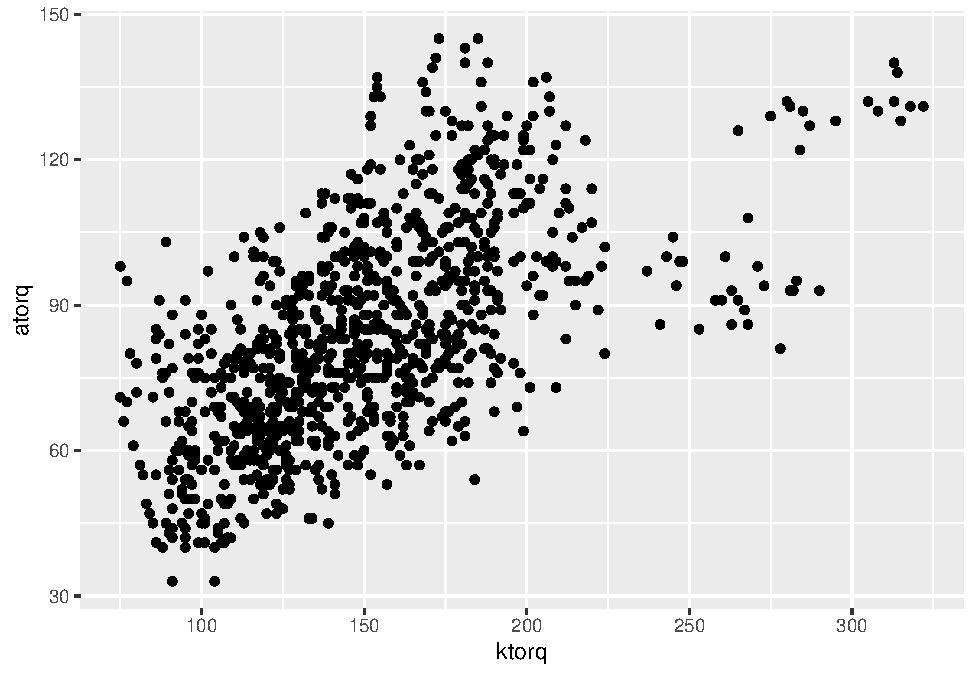
\includegraphics{07-visualization_files/figure-latex/simpleplot-1.pdf}
\caption{\label{fig:simpleplot}Simple plot}
\end{figure}

you get a plain, graphical representation of \emph{x} and \emph{y} as shown in Figure \ref{fig:simpleplot}.
You could adorn the graph with colors, a title, labels, a legend, text, and so forth, but
then the call to \texttt{ggplot} becomes more and more crowded, obscuring the
basic intention.

\begin{Shaded}
\begin{Highlighting}[]
\KeywordTok{ggplot}\NormalTok{(strn, }\KeywordTok{aes}\NormalTok{(ktorq, atorq)) }\OperatorTok{+}
\StringTok{  }\KeywordTok{geom_point}\NormalTok{() }\OperatorTok{+}
\StringTok{  }\KeywordTok{labs}\NormalTok{(}
    \DataTypeTok{title =} \StringTok{"Simple Plot Example"}\NormalTok{,}
    \DataTypeTok{subtitle =} \StringTok{"with a subtitle"}\NormalTok{,}
    \DataTypeTok{x =} \StringTok{"x-values"}\NormalTok{,}
    \DataTypeTok{y =} \StringTok{"y-values"}
\NormalTok{  ) }\OperatorTok{+}
\StringTok{  }\KeywordTok{theme}\NormalTok{(}\DataTypeTok{panel.background =} \KeywordTok{element_rect}\NormalTok{(}\DataTypeTok{fill =} \StringTok{"white"}\NormalTok{, }\DataTypeTok{colour =} \StringTok{"grey50"}\NormalTok{))}
\end{Highlighting}
\end{Shaded}

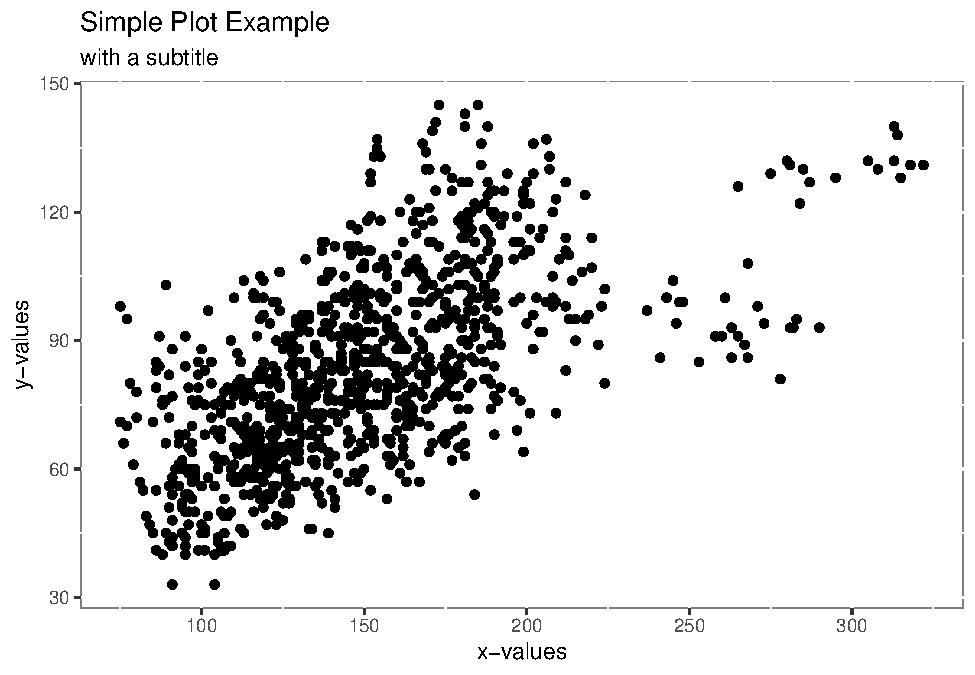
\includegraphics{07-visualization_files/figure-latex/complicatedplot-1.pdf}
The resulting plot is shown in Figure \ref{fig:complicatedplot}. We want to keep the recipes clean, so we emphasize the basic plot and then show later how to add adornments.

\hypertarget{notes-on-ggplot2-basics}{%
\subsection*{Notes on ggplot2 basics}\label{notes-on-ggplot2-basics}}
\addcontentsline{toc}{subsection}{Notes on ggplot2 basics}

While the package is called \texttt{ggplot2}, the primary plotting function in the package is called \texttt{ggplot}. It is important to understand the basic pieces of a \texttt{ggplot2} graph. In the preceding examples, you can see that we pass data into \texttt{ggplot}, then define how the graph is created by stacking together small phrases that describe some aspect of the plot. This stacking together of phrases is part of the ``grammar of graphics'' ethos (that's where the \texttt{gg} comes from).
To learn more, you can read \href{http://vita.had.co.nz/papers/layered-grammar.pdf}{``A Layered Grammar of Graphics''} written by \texttt{ggplot2} author Hadley Wickham.
The ``grammar of graphics'' concept originated with Leland Wilkinson, who articulated the idea of building graphics up from a set of primitives (i.e., verbs and nouns). With \texttt{ggplot}, the underlying data need not be fundamentally reshaped for each type of graphical representation. In general, the data stays the same and the user then changes syntax slightly to illustrate the data differently. This is significantly more consistent than base graphics, which often require reshaping the data in order to change the way it is visualized.

As we talk about \texttt{ggplot} graphics, it's worth defining the components of a \texttt{ggplot} graph:

\begin{description}
\item[\texttt{geometric\ object\ functions}]
These are geometric objects that describe the type of graph being created. These start with \texttt{geom\_} and examples include \texttt{geom\_line}, \texttt{geom\_boxplot}, and \texttt{geom\_point,} along with dozens more.
\item[\texttt{aesthetics}]
The aesthetics, or aesthetic mappings, communicate to \texttt{ggplot} which fields in the source data get mapped to which visual elements in the graphic. This is the \texttt{aes} line in a \texttt{ggplot} call.
\item[\texttt{stats}]
Stats are statistical transformations that are done before displaying the data. Not all graphs will have stats, but a few common stats are \texttt{stat\_ecdf} (the empirical cumulative distribution function) and \texttt{stat\_identity}, which tells \texttt{ggplot} to pass the data without doing any stats at all.
\item[\texttt{facet\ functions}]
Facets are subplots where each small plot represents a subgroup of the data. The faceting functions include \texttt{facet\_wrap} and \texttt{facet\_grid}.
\item[\texttt{themes}]
Themes are the visual elements of the plot that are not tied to data. These might include titles, margins, table of contents locations, or font choices.
\item[\texttt{layer}]
A layer is a combination of data, aesthetics, a geometric object, a stat, and other options to produce a visual layer in the \texttt{ggplot} graphic.
\end{description}

\hypertarget{long-versus-wide-data-with-ggplot}{%
\subsection*{``Long'' Versus ``Wide'' Data with ggplot}\label{long-versus-wide-data-with-ggplot}}
\addcontentsline{toc}{subsection}{``Long'' Versus ``Wide'' Data with ggplot}

One of the first sources of confusion for new \texttt{ggplot} users is that they are inclined to reshape their data to be ``wide'' before plotting it. ``Wide'' here means every variable they are plotting is its own column in the underlying data frame. This is an approach that many users develop while using Excel and then bring with them to R. \texttt{ggplot} works most easily with ``long'' data where additional variables are added as rows in the data frame rather than columns. The great side effect of adding more measurements as rows is that any properly constructed \texttt{ggplot} graphs will automatically update to reflect the new data without changing the \texttt{ggplot} code. If each additional variable were added as a column, then the plotting code would have to be changed to introduce additional variables. This idea of ``long'' versus ``wide'' data will become more obvious in the examples in the rest of this chapter.

\hypertarget{creating-a-scatter-plot}{%
\section{Creating a Scatter Plot}\label{creating-a-scatter-plot}}

We can plot the data by calling \texttt{ggplot}, passing in the data frame, and invoking a geometric point function:

\begin{Shaded}
\begin{Highlighting}[]
\KeywordTok{ggplot}\NormalTok{(strn, }\KeywordTok{aes}\NormalTok{(ktorq, atorq)) }\OperatorTok{+}
\StringTok{  }\KeywordTok{geom_point}\NormalTok{()}
\end{Highlighting}
\end{Shaded}

In this example, the data frame is called \texttt{strn} and the \emph{x} and \emph{y} data are in fields named \texttt{ktorq} and \texttt{atorq}, which we pass to the aesthetic in the call \texttt{aes(x,\ y)}.

A scatter plot is a common first attack on a new dataset. It's a quick
way to see the relationship, if any, between \emph{x} and \emph{y}.

Plotting with \texttt{ggplot} requires telling \texttt{ggplot} what data frame to use, then what type of graph to create, and which aesthetic mapping (\texttt{aes}) to use. The \texttt{aes} in this case defines which field from \texttt{df} goes into which axis on the plot. Then the command \texttt{geom\_point} communicates that you want a point graph, as opposed to a line or other type of graphic.

\hypertarget{cleaveland-dotplots}{%
\section{Cleaveland dotplots}\label{cleaveland-dotplots}}

One of the most important types of scatterplot is a cleaveland dotplot. It plots individual data points of a variable for every single row of your data. Useful for outlier detection, different spread of data a covariate.

\begin{Shaded}
\begin{Highlighting}[]
\CommentTok{# Save the figure into an object called f1}
\KeywordTok{ggplot}\NormalTok{(}\DataTypeTok{data =}\NormalTok{ strn) }\OperatorTok{+}\StringTok{ }
\StringTok{  }\KeywordTok{geom_point}\NormalTok{(}\KeywordTok{aes}\NormalTok{(}\DataTypeTok{y =} \KeywordTok{seq}\NormalTok{(}\DecValTok{1}\NormalTok{,}\KeywordTok{nrow}\NormalTok{(strn),}\DecValTok{1}\NormalTok{), }\DataTypeTok{x =}\NormalTok{ atorq)) }\OperatorTok{+}
\StringTok{  }\KeywordTok{ylab}\NormalTok{ (}\StringTok{"row number"}\NormalTok{) }\OperatorTok{+}\StringTok{ }\CommentTok{# Label you like}
\StringTok{  }\KeywordTok{xlab}\NormalTok{ (}\StringTok{"ankle torque"}\NormalTok{) }\CommentTok{# Label you like}
\end{Highlighting}
\end{Shaded}

\begin{figure}
\centering
\includegraphics{07-visualization_files/figure-latex/unnamed-chunk-5-1.pdf}
\caption{\label{fig:unnamed-chunk-5}Ankle torque by group and time}
\end{figure}

\hypertarget{adding-a-title-and-labels}{%
\section{Adding a Title and Labels}\label{adding-a-title-and-labels}}

You want to add a title to your plot or add labels for the axes.

With \texttt{ggplot} we add a \texttt{labs} element that controls the labels for the title and axes.

When calling \texttt{labs} in \texttt{ggplot}, specify:

\begin{description}
\item[\texttt{title}]
The desired title text
\item[\texttt{x}]
x-axis label
\item[\texttt{y}]
y-axis label
\end{description}

\begin{Shaded}
\begin{Highlighting}[]
\KeywordTok{ggplot}\NormalTok{(strn, }\KeywordTok{aes}\NormalTok{(ktorq, atorq)) }\OperatorTok{+}
\StringTok{  }\KeywordTok{geom_point}\NormalTok{() }\OperatorTok{+}
\StringTok{  }\KeywordTok{labs}\NormalTok{(}\DataTypeTok{title =} \StringTok{"The Title"}\NormalTok{,}
       \DataTypeTok{x =} \StringTok{"knee torque"}\NormalTok{,}
       \DataTypeTok{y =} \StringTok{"ankle torque"}\NormalTok{)}
\end{Highlighting}
\end{Shaded}

A title and better labels will make a graph more interesting and easier to interpret.

\hypertarget{adding-or-removing-a-grid}{%
\section{Adding (or Removing) a Grid}\label{adding-or-removing-a-grid}}

You want to change the background grid to your graphic.

With \texttt{ggplot} background grids come as a default, as you have seen in other recipes. However, we can alter the background grid using the \texttt{theme} function or by applying a prepackaged theme to our graph.
We can use \texttt{theme} to alter the background panel of our graphic:

\begin{Shaded}
\begin{Highlighting}[]
\KeywordTok{ggplot}\NormalTok{(strn, }\KeywordTok{aes}\NormalTok{(ktorq, atorq)) }\OperatorTok{+}
\StringTok{  }\KeywordTok{geom_point}\NormalTok{() }\OperatorTok{+}
\StringTok{  }\KeywordTok{theme}\NormalTok{(}\DataTypeTok{panel.background =} \KeywordTok{element_rect}\NormalTok{(}\DataTypeTok{fill =} \StringTok{"white"}\NormalTok{, }\DataTypeTok{colour =} \StringTok{"grey50"}\NormalTok{))}
\end{Highlighting}
\end{Shaded}

\begin{figure}
\centering
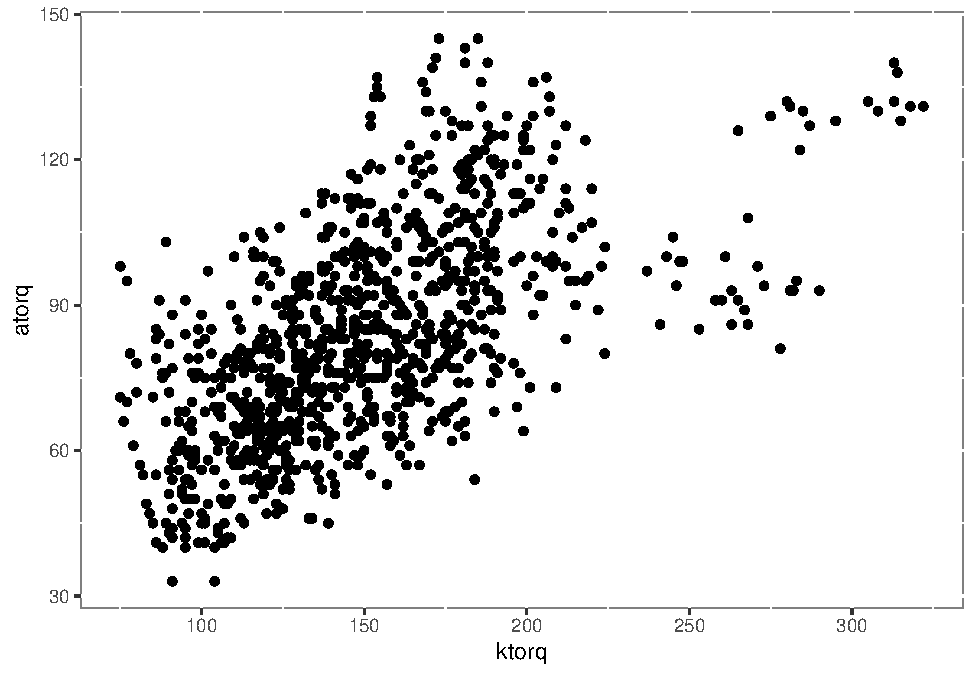
\includegraphics{07-visualization_files/figure-latex/whitebackground-1.pdf}
\caption{\label{fig:whitebackground}White background}
\end{figure}

\texttt{ggplot} fills in the background with a grey grid by default. So you may find yourself wanting to remove that grid completely or change it to something else. Let's create a \texttt{ggplot} graphic and then incrementally change the background style.

We can add or change aspects of our graphic by creating a \texttt{ggplot} object, then calling the object and using the \texttt{+} to add to it. The background shading in a \texttt{ggplot} graphic is actually three different graph elements:

\texttt{panel.grid.major}:

These are white by default and heavy.

\texttt{panel.grid.minor}:

These are white by default and light.

\texttt{panel.background}:

\hypertarget{applying-a-theme-to-a-ggplot-figure}{%
\section{Applying a Theme to a ggplot Figure}\label{applying-a-theme-to-a-ggplot-figure}}

You want your plot to use a preset collection of colors, styles, and formatting.

\texttt{ggplot} supports \emph{themes}, which are collections of settings for your figures. To use one of the themes, just add the desired theme function to your \texttt{ggplot} with a \texttt{+}:

\begin{Shaded}
\begin{Highlighting}[]
\KeywordTok{ggplot}\NormalTok{(strn, }\KeywordTok{aes}\NormalTok{(ktorq, atorq)) }\OperatorTok{+}
\StringTok{  }\KeywordTok{geom_point}\NormalTok{() }\OperatorTok{+}
\StringTok{  }\KeywordTok{theme_bw}\NormalTok{()}
\end{Highlighting}
\end{Shaded}

The \texttt{ggplot2} package contains the following themes Figure \ref{fig:ggthemes}:

\begin{verbatim}
theme_bw()
theme_dark() 
theme_classic()
theme_gray()
theme_linedraw()
theme_light()
theme_minimal()
theme_test()
theme_void()
\end{verbatim}

\begin{figure}

{\centering 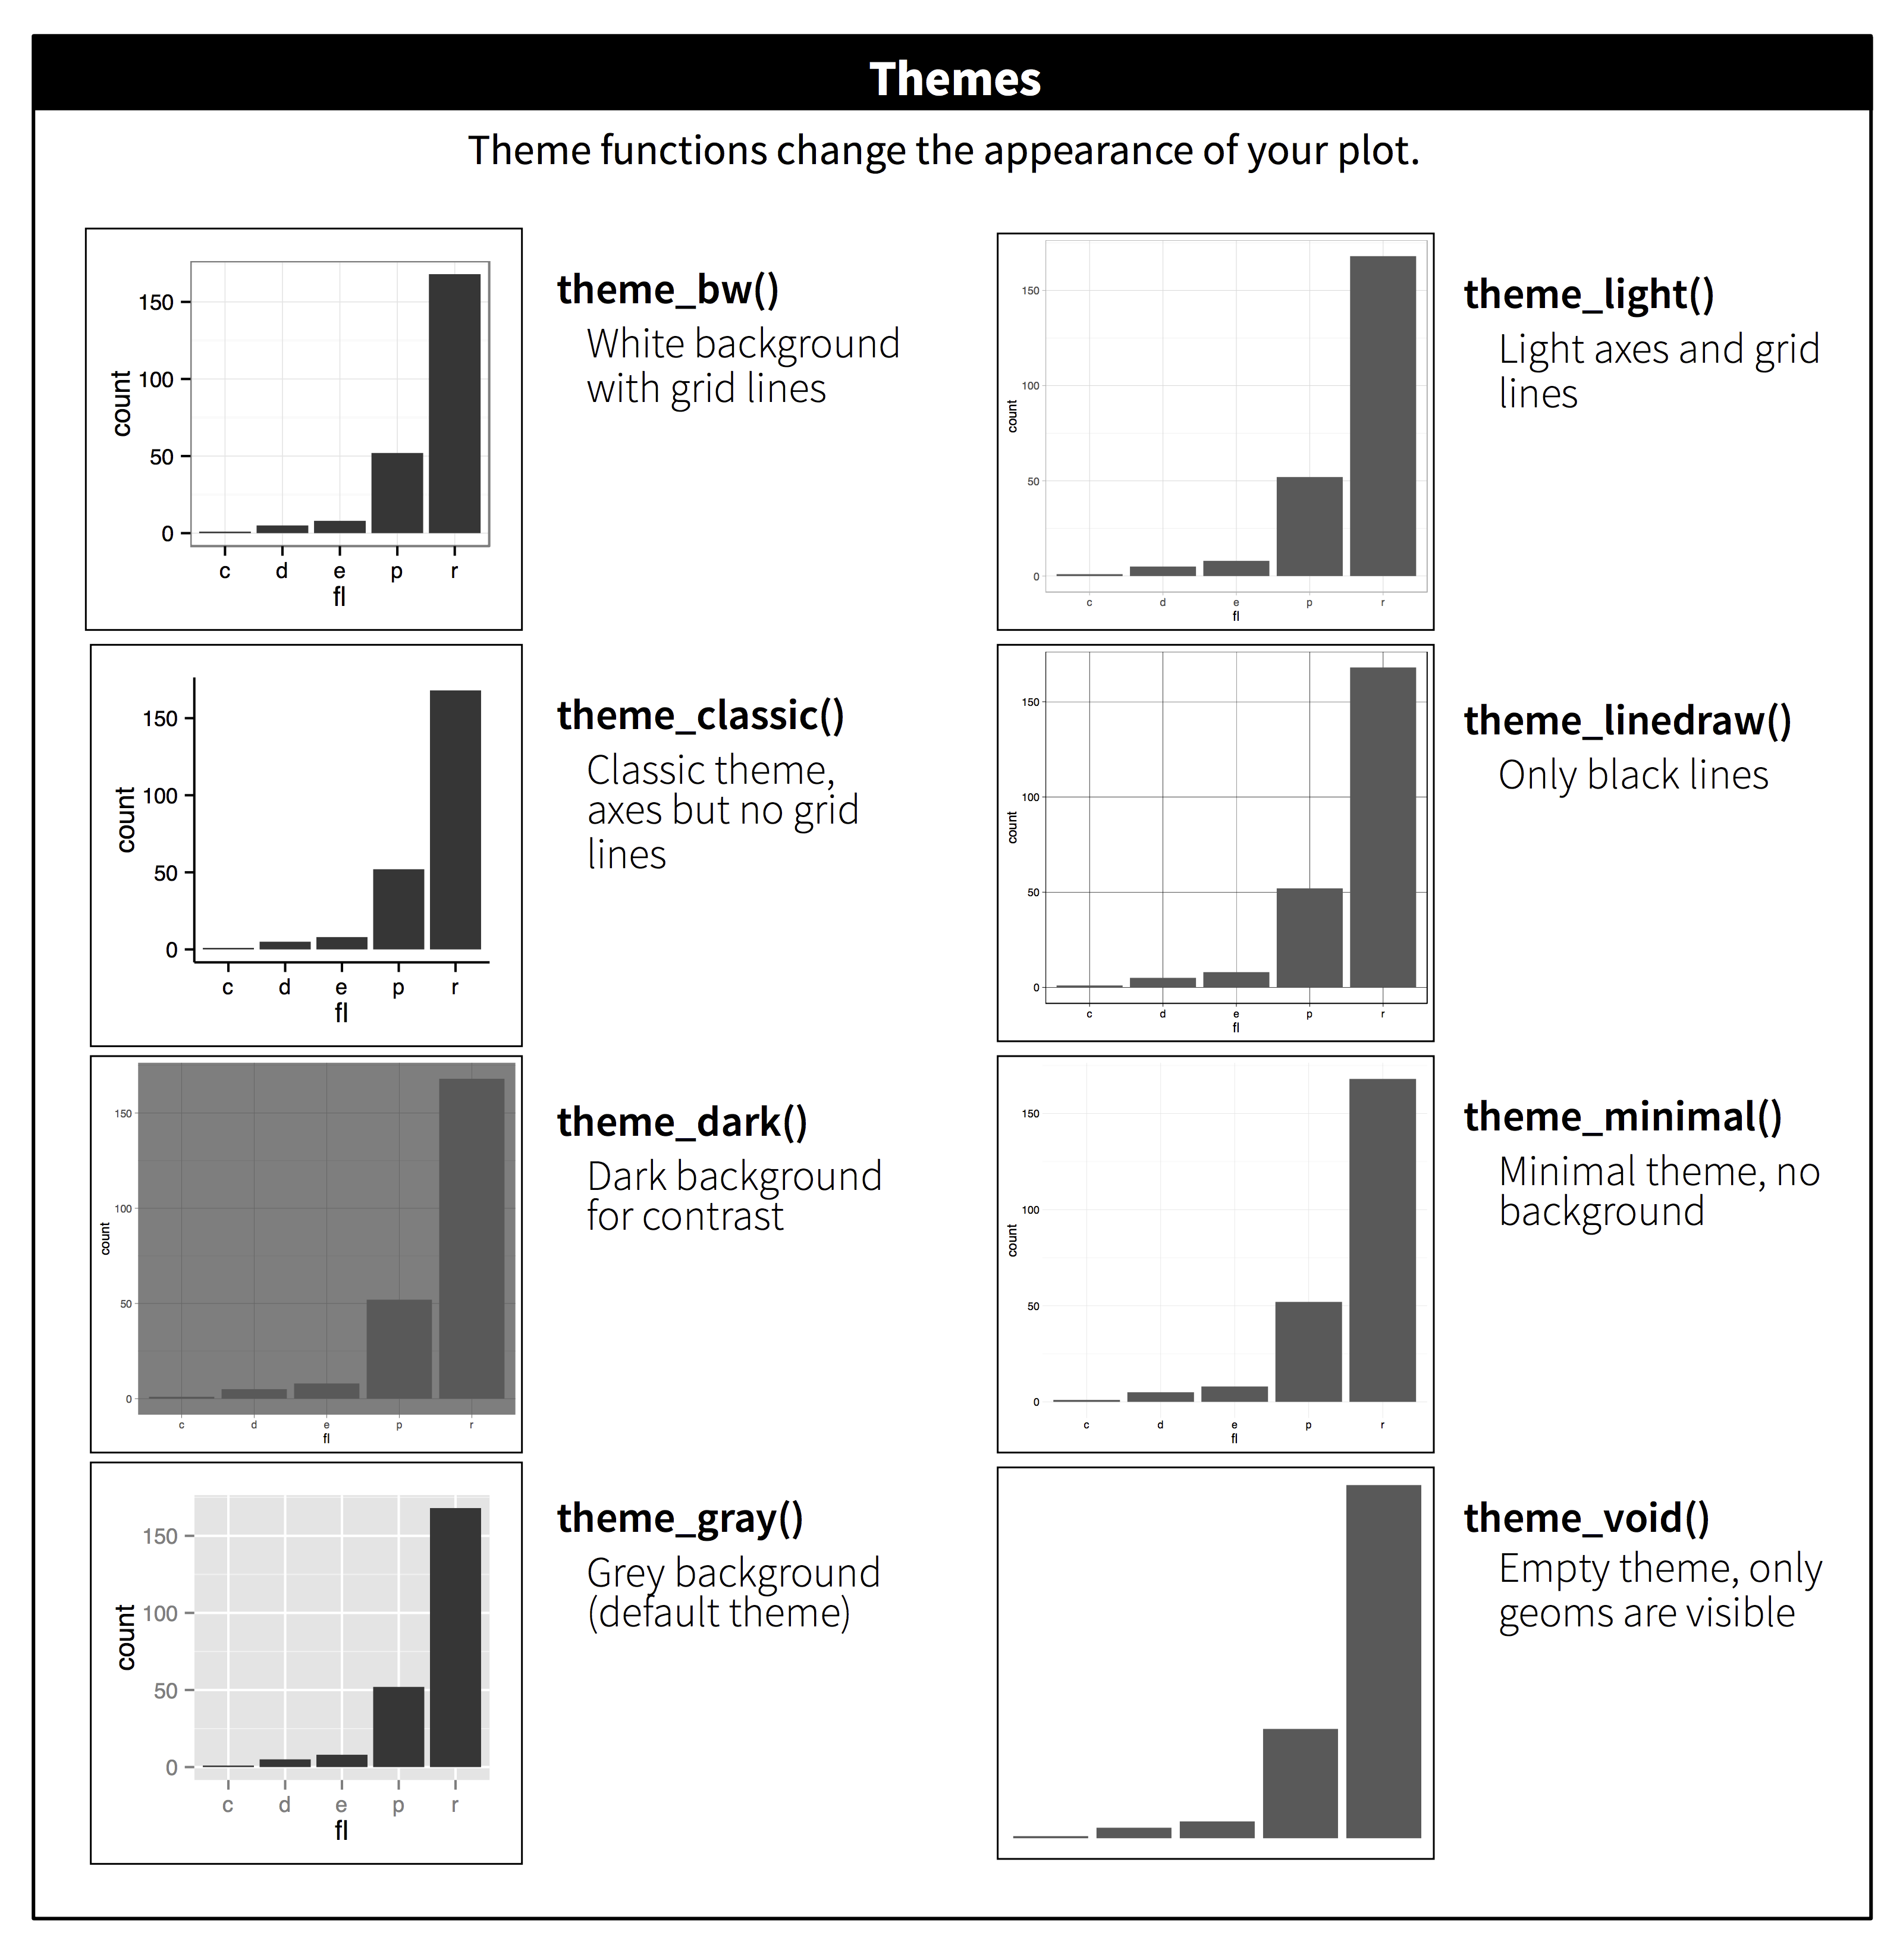
\includegraphics[width=0.5\linewidth]{images/visualization-themes} 

}

\caption{Default themes in ggplot.}\label{fig:ggthemes}
\end{figure}

\hypertarget{creating-a-scatter-plot-of-multiple-groups}{%
\section{Creating a Scatter Plot of Multiple Groups}\label{creating-a-scatter-plot-of-multiple-groups}}

You have data in a data frame with multiple observations per record: \emph{x}, \emph{y}, and a
factor \emph{f} that indicates the group. You want to create a scatter
plot of \emph{x} and \emph{y} that distinguishes among the groups.

With \texttt{ggplot} we control the mapping of shapes to the factor \texttt{group} by passing \texttt{shape\ =\ group} to the \texttt{aes}.

\begin{Shaded}
\begin{Highlighting}[]
\KeywordTok{ggplot}\NormalTok{(strn, }\KeywordTok{aes}\NormalTok{(ktorq, atorq, }\DataTypeTok{shape =}\NormalTok{ group)) }\OperatorTok{+}
\StringTok{  }\KeywordTok{geom_point}\NormalTok{()}
\end{Highlighting}
\end{Shaded}

Plotting multiple groups in one scatter plot creates an uninformative
mess unless we distinguish one group from another. We make this distinction in \texttt{ggplot} by setting the \texttt{shape} parameter of the \texttt{aes} function.

We can add \texttt{shape\ =\ group} and \texttt{color\ =\ group} to our \texttt{aes} call, to get each species with a different shape and color, shown in Figure \ref{fig:strnshape}.

\begin{Shaded}
\begin{Highlighting}[]
\KeywordTok{ggplot}\NormalTok{(strn, }\KeywordTok{aes}\NormalTok{(ktorq, atorq, }\DataTypeTok{shape =}\NormalTok{ group, }\DataTypeTok{color =}\NormalTok{group)) }\OperatorTok{+}
\StringTok{  }\KeywordTok{geom_point}\NormalTok{()}
\end{Highlighting}
\end{Shaded}

\begin{figure}
\centering
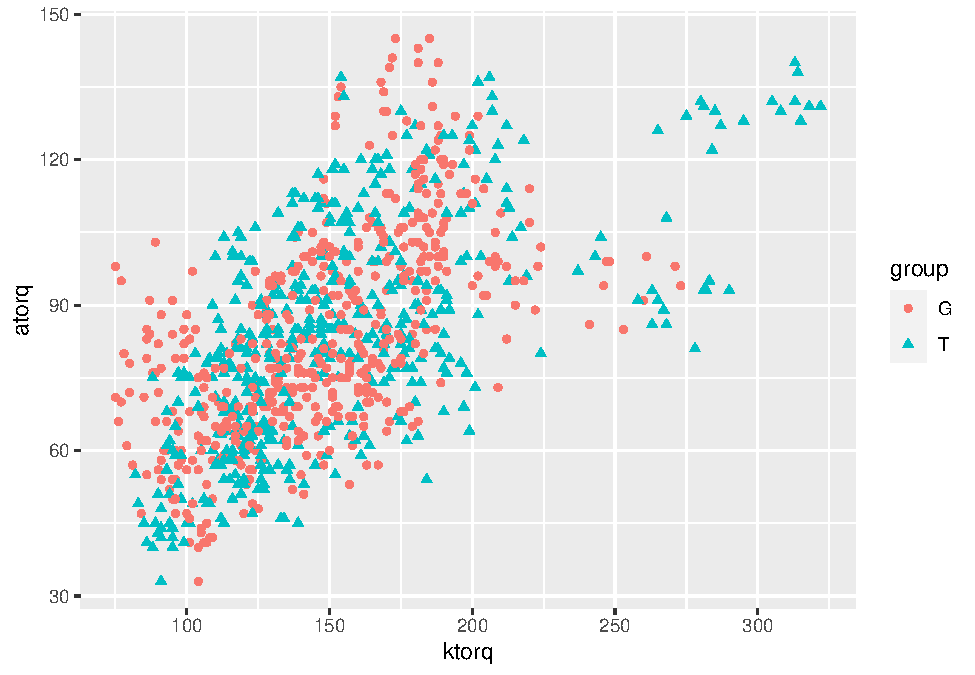
\includegraphics{07-visualization_files/figure-latex/strnshape-1.pdf}
\caption{\label{fig:strnshape}strength: shape and color}
\end{figure}

\texttt{ggplot} conveniently sets up a legend for you as well, which is handy.

\hypertarget{adding-or-removing-a-legend}{%
\section{Adding (or Removing) a Legend}\label{adding-or-removing-a-legend}}

You want your plot to include a \emph{legend}, the little box that decodes
the graphic for the viewer.

In most cases \texttt{ggplot} will add the legends automatically, as you can see in the previous recipe. If you do not have explicit grouping in the \texttt{aes}, then \texttt{ggplot} will not show a legend by default. If we want to force \texttt{ggplot} to show a legend, we can set the shape or line type of our graph to a constant. \texttt{ggplot} will then show a legend with one group. We then use \texttt{guides} to guide \texttt{ggplot} in how to label the legend.

This can be illustrated with our \texttt{strn} scatter plot:

\begin{Shaded}
\begin{Highlighting}[]
\KeywordTok{ggplot}\NormalTok{(strn, }\KeywordTok{aes}\NormalTok{(ktorq, atorq, }\DataTypeTok{color =}\NormalTok{group)) }\OperatorTok{+}
\StringTok{  }\KeywordTok{geom_point}\NormalTok{() }\OperatorTok{+}
\StringTok{  }\KeywordTok{guides}\NormalTok{(}\DataTypeTok{color =}\KeywordTok{guide_legend}\NormalTok{(}\DataTypeTok{title=}\StringTok{"My Legend Title"}\NormalTok{)) }
\end{Highlighting}
\end{Shaded}

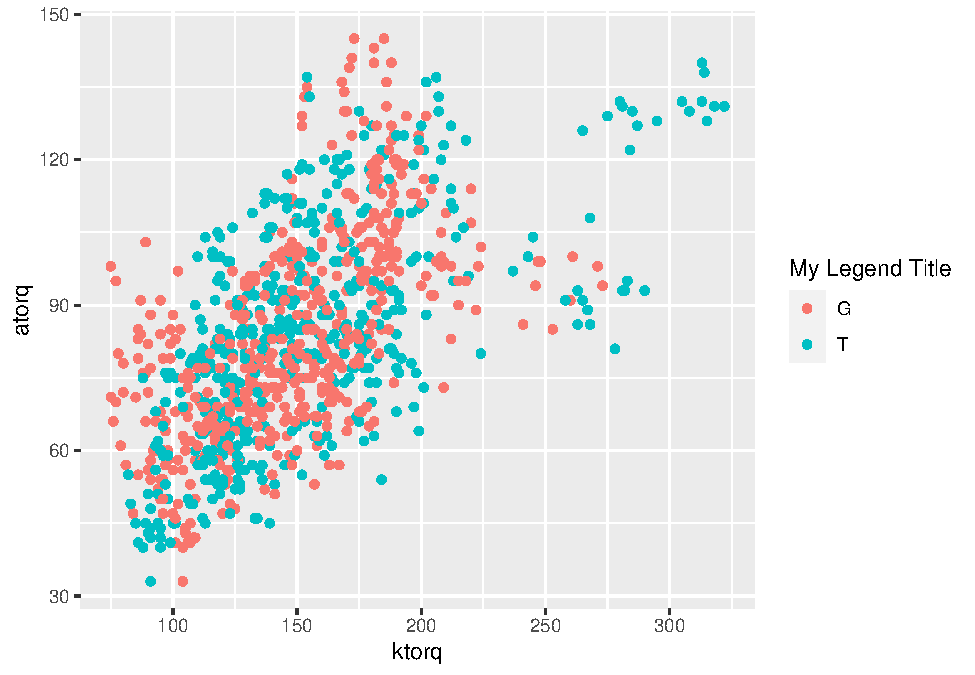
\includegraphics{07-visualization_files/figure-latex/needslegend-1.pdf}
Figure \ref{fig:needslegend} illustrates the result of setting the shape to a string value and then relabeling the legend using \texttt{guides}.

More commonly, you may want to turn legends off, which you can do by setting the \texttt{legend.position\ =\ "none"} in the \texttt{theme}. We can use the \texttt{strn} plot from the prior recipe and add the \texttt{theme} call as shown in Figure \ref{fig:shapelegend}:

\begin{Shaded}
\begin{Highlighting}[]
\KeywordTok{ggplot}\NormalTok{(strn, }\KeywordTok{aes}\NormalTok{(ktorq, atorq, }\DataTypeTok{color =}\NormalTok{group)) }\OperatorTok{+}
\StringTok{  }\KeywordTok{geom_point}\NormalTok{() }\OperatorTok{+}
\StringTok{  }\KeywordTok{theme}\NormalTok{(}\DataTypeTok{legend.position =} \StringTok{"none"}\NormalTok{)}
\end{Highlighting}
\end{Shaded}

\begin{figure}
\centering
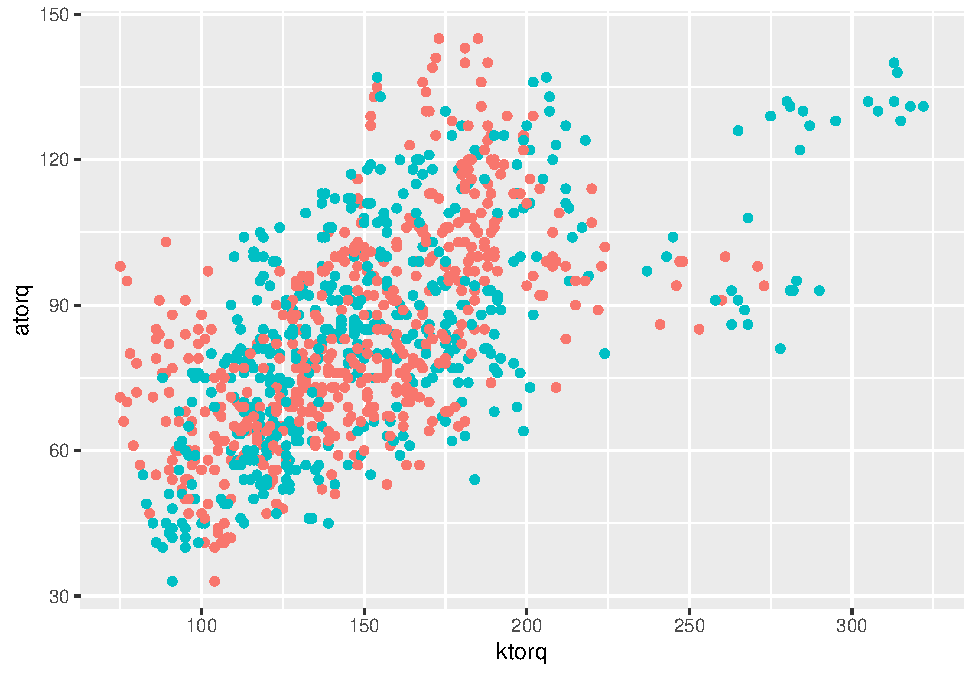
\includegraphics{07-visualization_files/figure-latex/shapelegend-1.pdf}
\caption{\label{fig:shapelegend}Legend removed}
\end{figure}

Adding legends to \texttt{ggplot} when there is no grouping is an exercise in ``tricking'' \texttt{ggplot} into showing the legend by passing a string to a grouping parameter in \texttt{aes}. While this will not change the grouping (as there is only one group), it will result in a legend being shown with a name.

Then we can use \texttt{guides} to alter the legend title. It's worth noting that we are not changing anything about the data, just exploiting settings in order to coerce \texttt{ggplot} into showing a legend when it typically would not.

One of the huge benefits of \texttt{ggplot} is its very good defaults. Getting positions and correspondence between labels and their point types is done automatically, but can be overridden if needed. To remove a legend totally, we set \texttt{theme} parameters with \texttt{theme(legend.position\ =\ "none")}. In addition to \texttt{"none"} you can set the \texttt{legend.position} to be \texttt{"left"}, \texttt{"right"}, \texttt{"bottom"}, \texttt{"top"}, or a two-element numeric vector. Use a two-element numeric vector in order to pass \texttt{ggplot} specific coordinates of where you want the legend. If you're using the coordinate positions, the values passed are between 0 and 1 for the \emph{x} and \emph{y} position, respectively.

Figure \ref{fig:shapelegend-moved} shows an example of a legend positioned at the bottom, created with this adjustment to the \texttt{legend.position}:

\begin{Shaded}
\begin{Highlighting}[]
\KeywordTok{ggplot}\NormalTok{(strn, }\KeywordTok{aes}\NormalTok{(ktorq, atorq, }\DataTypeTok{color =}\NormalTok{group)) }\OperatorTok{+}
\StringTok{  }\KeywordTok{geom_point}\NormalTok{() }\OperatorTok{+}\StringTok{ }
\StringTok{  }\KeywordTok{theme}\NormalTok{(}\DataTypeTok{legend.position =} \StringTok{"bottom"}\NormalTok{)}
\end{Highlighting}
\end{Shaded}

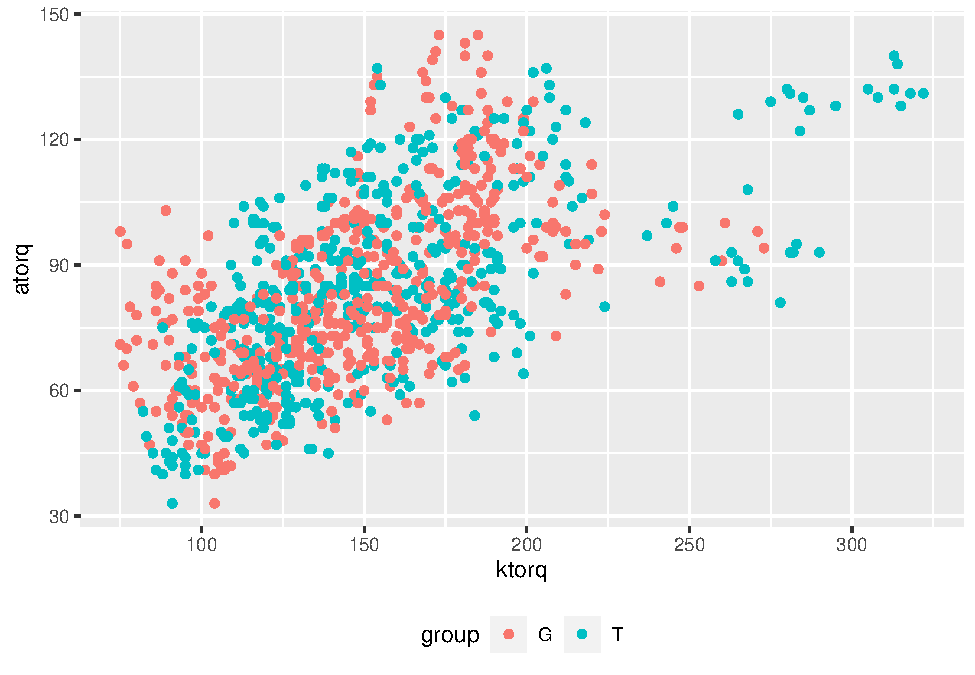
\includegraphics{07-visualization_files/figure-latex/shapelegend-moved-1.pdf}
Or we could use the two-element numeric vector to put the legend in a specific location, as in Figure \ref{fig:shapelegend-moved2}. The example puts the center of the legend at 80\% to the right and 20\% up from the bottom.

\begin{Shaded}
\begin{Highlighting}[]
\KeywordTok{ggplot}\NormalTok{(strn, }\KeywordTok{aes}\NormalTok{(ktorq, atorq, }\DataTypeTok{color =}\NormalTok{group)) }\OperatorTok{+}
\StringTok{  }\KeywordTok{geom_point}\NormalTok{() }\OperatorTok{+}\StringTok{ }
\StringTok{  }\KeywordTok{theme}\NormalTok{(}\DataTypeTok{legend.position =} \KeywordTok{c}\NormalTok{(.}\DecValTok{8}\NormalTok{, }\FloatTok{.2}\NormalTok{))}
\end{Highlighting}
\end{Shaded}

\begin{figure}
\centering
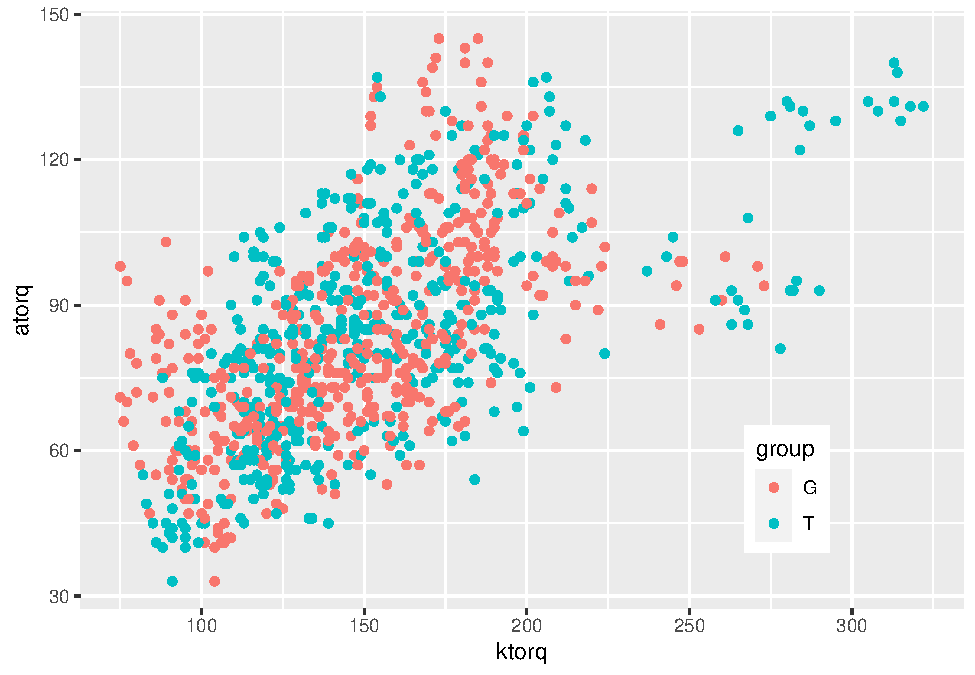
\includegraphics{07-visualization_files/figure-latex/shapelegend-moved2-1.pdf}
\caption{\label{fig:shapelegend-moved2}Legend at a point}
\end{figure}

In many aspects beyond legends, \texttt{ggplot} uses sane defaults but offers the flexibility to override them and tweak the details. You can find more details on \texttt{ggplot} options related to legends in the help for \texttt{theme} by typing \texttt{**?theme**} or looking in the \texttt{ggplot} \href{http://ggplot2.tidyverse.org/reference/theme.html}{online reference material}.

\hypertarget{creating-one-scatter-plot-for-each-group}{%
\section{Creating One Scatter Plot for Each Group}\label{creating-one-scatter-plot-for-each-group}}

Your dataset contains (at least) two numeric variables and a factor or character field defining a group. You want to create several scatter plots for the numeric variables, with one
scatter plot for each level of the factor or character field.

We produce this kind of plot, called a \emph{conditioning plot}, in \texttt{ggplot} by adding \texttt{facet\_wrap} to our plot.
In this example we use the data frame \texttt{strn}, which contains three columns: \emph{x}, \emph{y}, and \emph{f}, with \emph{f} being a factor (or a character string).

\begin{Shaded}
\begin{Highlighting}[]
\KeywordTok{ggplot}\NormalTok{(strn, }\KeywordTok{aes}\NormalTok{(ktorq, atorq)) }\OperatorTok{+}
\StringTok{  }\KeywordTok{geom_point}\NormalTok{() }\OperatorTok{+}
\StringTok{  }\KeywordTok{facet_wrap}\NormalTok{( }\OperatorTok{~}\StringTok{ }\NormalTok{group)}
\end{Highlighting}
\end{Shaded}

\hypertarget{creating-a-bar-chart}{%
\section{Creating a Bar Chart}\label{creating-a-bar-chart}}

You want to create a bar chart.

A common situation is to have a column of data that represents a group and then another column that represents a measure about that group. This format is ``long'' data because the data runs vertically instead of having a column for each group.

Using the \texttt{geom\_bar} function in \texttt{ggplot}, we can plot the heights as bars. If the data is already aggregated, we add \texttt{stat\ =\ "identity"} so that \texttt{ggplot} knows it needs to do no aggregation on the groups of values before plotting.

The first thing to do when trying to generate nice plots is to create a dataframe of the values you want to plot. In this case, since I want to plot the mean group by time values of \texttt{ktorq}, and include one standard deviation error bars, I need to generate these values.

In \texttt{ggplot} we can use the \texttt{fill} parameter in \texttt{aes} to tell \texttt{ggplot} what field to base the colors on. If we pass a numeric field to \texttt{ggplot}, we will get a continuous gradient of colors; and if we pass a factor or character field to \texttt{fill}, we will get contrasting colors for each group.

\begin{Shaded}
\begin{Highlighting}[]
\CommentTok{# generate a summarized dataframe }
\NormalTok{df.plot =}\StringTok{ }\NormalTok{strn }\OperatorTok
\StringTok{  }\KeywordTok{group_by}\NormalTok{(group, time) }\OperatorTok
\StringTok{  }\KeywordTok{summarize}\NormalTok{ (}\DataTypeTok{Mean =} \KeywordTok{mean}\NormalTok{ (ktorq, }\DataTypeTok{na.rm =}\NormalTok{ T), }\CommentTok{# change ktorq to other variables you desire}
             \DataTypeTok{Sd =} \KeywordTok{sd}\NormalTok{ (ktorq, }\DataTypeTok{na.rm =}\NormalTok{ T)) }\OperatorTok
\StringTok{  }\KeywordTok{ungroup}\NormalTok{()}

\CommentTok{# Combined plot}
\KeywordTok{ggplot}\NormalTok{(}\DataTypeTok{data =}\NormalTok{ df.plot) }\OperatorTok{+}\StringTok{ }
\KeywordTok{geom_bar}\NormalTok{ (}\KeywordTok{aes}\NormalTok{(}\DataTypeTok{y =}\NormalTok{ Mean, }\DataTypeTok{x =}\NormalTok{ group, }\DataTypeTok{fill =}\NormalTok{ time), }\DataTypeTok{stat =} \StringTok{"identity"}\NormalTok{, }\DataTypeTok{color=}\StringTok{"black"}\NormalTok{, }\DataTypeTok{position=}\KeywordTok{position_dodge}\NormalTok{()) }\OperatorTok{+}
\KeywordTok{ylab}\NormalTok{ (}\StringTok{"Knee torque"}\NormalTok{) }\OperatorTok{+}
\KeywordTok{xlab}\NormalTok{ (}\StringTok{"Group"}\NormalTok{)}
\end{Highlighting}
\end{Shaded}

\begin{figure}
\centering
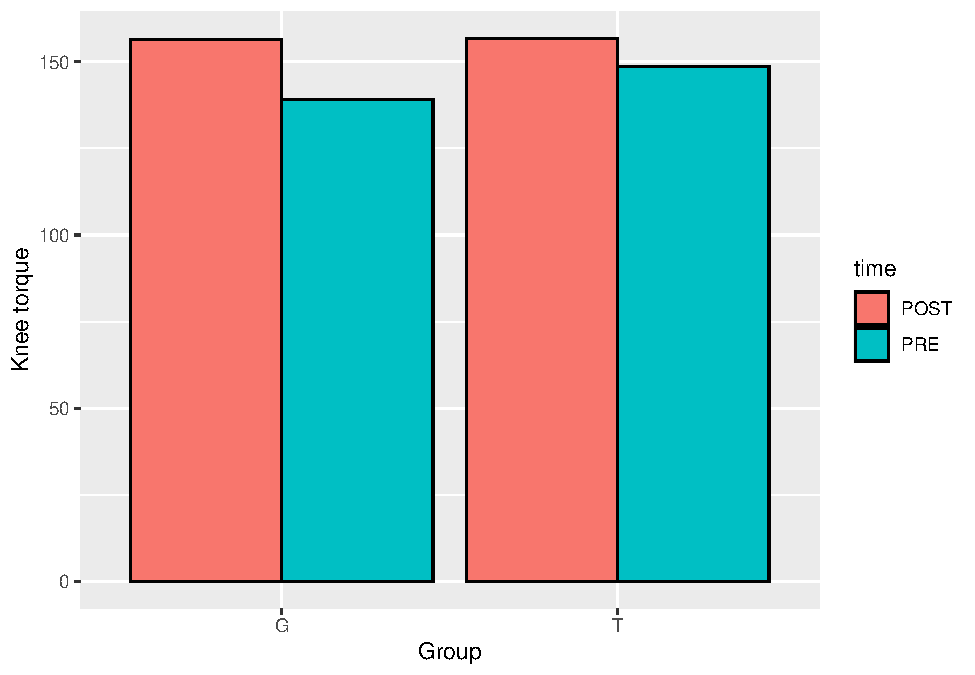
\includegraphics{07-visualization_files/figure-latex/ktorqbar-1.pdf}
\caption{\label{fig:ktorqbar}Knee torque by group}
\end{figure}

Figure \ref{fig:ktorqbar} shows the resulting bar chart.

This example uses \texttt{stat\ =\ "identity"}, which assumes that the heights of your bars are conveniently stored as a value in one field with only one record per column.

\hypertarget{adding-standard-deviation-error-bars-to-a-bar-chart}{%
\section{Adding standard deviation error bars to a Bar Chart}\label{adding-standard-deviation-error-bars-to-a-bar-chart}}

You want to augment a bar chart with standard deviation.

\begin{Shaded}
\begin{Highlighting}[]
\KeywordTok{ggplot}\NormalTok{(}\DataTypeTok{data =}\NormalTok{ df.plot) }\OperatorTok{+}\StringTok{ }
\KeywordTok{geom_bar}\NormalTok{ (}\KeywordTok{aes}\NormalTok{(}\DataTypeTok{y =}\NormalTok{ Mean, }\DataTypeTok{x =}\NormalTok{ group, }\DataTypeTok{fill =}\NormalTok{ time), }\DataTypeTok{stat =} \StringTok{"identity"}\NormalTok{, }\DataTypeTok{color=}\StringTok{"black"}\NormalTok{, }\DataTypeTok{position=}\KeywordTok{position_dodge}\NormalTok{()) }\OperatorTok{+}
\KeywordTok{geom_errorbar}\NormalTok{(}\KeywordTok{aes}\NormalTok{(}\DataTypeTok{ymin=}\NormalTok{Mean }\OperatorTok{-}\NormalTok{Sd, }\DataTypeTok{ymax=}\NormalTok{Mean }\OperatorTok{+}\NormalTok{Sd, }\DataTypeTok{x =}\NormalTok{ group, }\DataTypeTok{colour =}\NormalTok{ time), }
              \DataTypeTok{width=}\NormalTok{.}\DecValTok{2}\NormalTok{,}
               \DataTypeTok{position=}\KeywordTok{position_dodge}\NormalTok{(}\FloatTok{0.9}\NormalTok{)) }\OperatorTok{+}
\KeywordTok{ylab}\NormalTok{ (}\StringTok{"Knee torque"}\NormalTok{) }\OperatorTok{+}
\KeywordTok{xlab}\NormalTok{ (}\StringTok{"Group"}\NormalTok{)}
\end{Highlighting}
\end{Shaded}

\begin{figure}
\centering
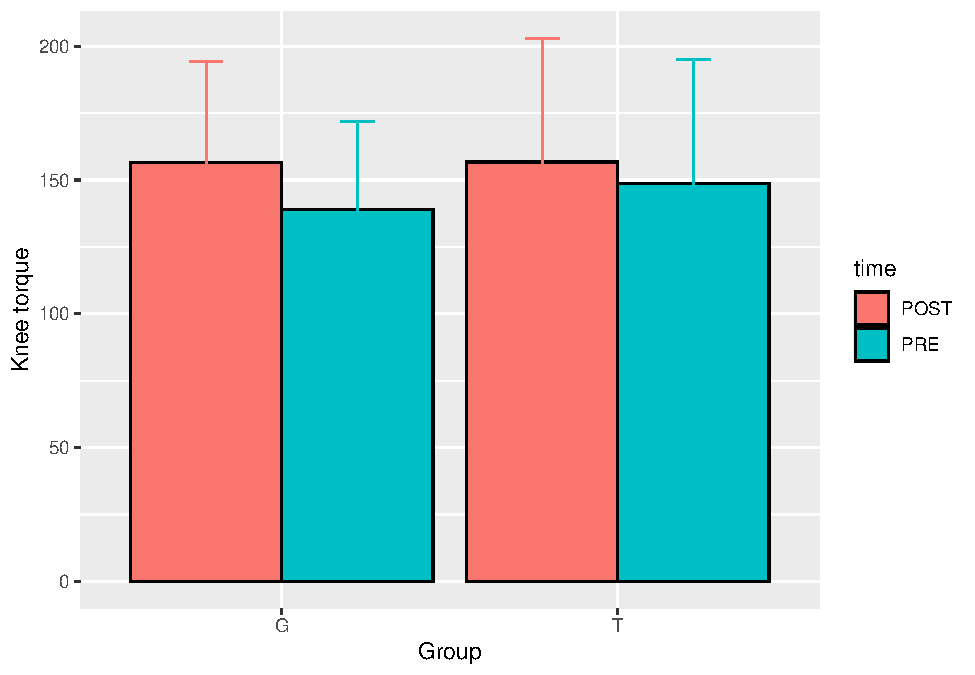
\includegraphics{07-visualization_files/figure-latex/ktorqbarerrors-1.pdf}
\caption{\label{fig:ktorqbarerrors}Knee torque by group with error bars as 1SD}
\end{figure}

\hypertarget{custom-coloring-a-bar-chart}{%
\section{Custom coloring a Bar Chart}\label{custom-coloring-a-bar-chart}}

You want to manually customize the color or shade the bars of a bar chart.

We can customize the colour using the \texttt{scale\_fill\_manual} and/or the \texttt{scale\_colour\_manual} commands. When you include \texttt{fill} in \texttt{aes}, customize the colour using \texttt{scale\_fill\_manual}, and if you include \texttt{colour} in \texttt{aes}, customize using \texttt{scale\_colour\_manual}. You can change colours by keying in the actual names of different colours after the \texttt{value} command. The order of colours matches the order of levels in the factor.{[}This is a link of the myriad colours and their names available in ggplot{]} (\url{http://sape.inf.usi.ch/quick-reference/ggplot2/colour})

\begin{Shaded}
\begin{Highlighting}[]
\KeywordTok{ggplot}\NormalTok{(}\DataTypeTok{data =}\NormalTok{ df.plot) }\OperatorTok{+}\StringTok{ }
\KeywordTok{geom_bar}\NormalTok{ (}\KeywordTok{aes}\NormalTok{(}\DataTypeTok{y =}\NormalTok{ Mean, }\DataTypeTok{x =}\NormalTok{ group, }\DataTypeTok{fill =}\NormalTok{ time), }\DataTypeTok{stat =} \StringTok{"identity"}\NormalTok{, }\DataTypeTok{color=}\StringTok{"black"}\NormalTok{, }\DataTypeTok{position=}\KeywordTok{position_dodge}\NormalTok{()) }\OperatorTok{+}
\KeywordTok{geom_errorbar}\NormalTok{(}\KeywordTok{aes}\NormalTok{(}\DataTypeTok{ymin=}\NormalTok{Mean }\OperatorTok{-}\NormalTok{Sd, }\DataTypeTok{ymax=}\NormalTok{Mean }\OperatorTok{+}\NormalTok{Sd, }\DataTypeTok{x =}\NormalTok{ group, }\DataTypeTok{colour =}\NormalTok{ time), }
              \DataTypeTok{width=}\NormalTok{.}\DecValTok{2}\NormalTok{,}
               \DataTypeTok{position=}\KeywordTok{position_dodge}\NormalTok{(}\FloatTok{0.9}\NormalTok{)) }\OperatorTok{+}
\KeywordTok{scale_fill_manual}\NormalTok{(}\DataTypeTok{values =} \KeywordTok{c}\NormalTok{(}\StringTok{"blue"}\NormalTok{, }\StringTok{"red"}\NormalTok{)) }\OperatorTok{+}
\KeywordTok{scale_colour_manual}\NormalTok{(}\DataTypeTok{values =} \KeywordTok{c}\NormalTok{(}\StringTok{"blue"}\NormalTok{, }\StringTok{"red"}\NormalTok{)) }\OperatorTok{+}
\KeywordTok{ylab}\NormalTok{ (}\StringTok{"Knee torque"}\NormalTok{) }\OperatorTok{+}
\KeywordTok{xlab}\NormalTok{ (}\StringTok{"Group"}\NormalTok{)}
\end{Highlighting}
\end{Shaded}

\begin{figure}
\centering
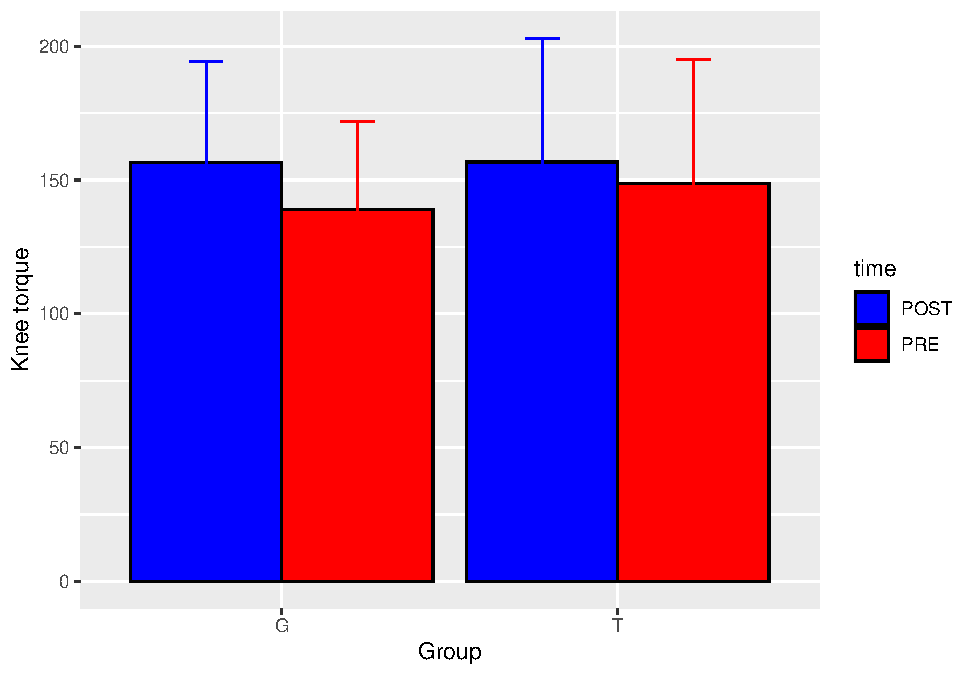
\includegraphics{07-visualization_files/figure-latex/customcol-1.pdf}
\caption{\label{fig:customcol}Knee torque by group with error bars as 1SD}
\end{figure}

\hypertarget{histogram}{%
\section{Histogram}\label{histogram}}

Useful for outlier detection, different spread of data a covariate

Knee torque by group and time

The \texttt{geom\_histogram} function must decide how many cells (bins) to create for
binning the data. In this example, the default algorithm chose 30
bins. If we wanted fewer bins, we would include the \texttt{bins} parameter to tell \texttt{geom\_histogram} how many bins we want:

\begin{Shaded}
\begin{Highlighting}[]
\KeywordTok{ggplot}\NormalTok{(}\DataTypeTok{data =}\NormalTok{ strn) }\OperatorTok{+}
\KeywordTok{geom_histogram}\NormalTok{(}\KeywordTok{aes}\NormalTok{(}\DataTypeTok{x =}\NormalTok{ ktorq, }\DataTypeTok{fill =}\NormalTok{ group), }\DataTypeTok{binwidth =} \DecValTok{10}\NormalTok{) }\OperatorTok{+}\StringTok{ }\CommentTok{# try binwidth of 0.1, 1, 10, 100}
\KeywordTok{facet_wrap}\NormalTok{(  }\OperatorTok{~}\StringTok{ }\NormalTok{time, }\DataTypeTok{scales =} \StringTok{"fixed"}\NormalTok{) }\OperatorTok{+}
\KeywordTok{ylab}\NormalTok{ (}\StringTok{"Frequency"}\NormalTok{) }\OperatorTok{+}
\KeywordTok{xlab}\NormalTok{ (}\StringTok{"knee torque"}\NormalTok{)}
\end{Highlighting}
\end{Shaded}

\begin{figure}
\centering
\includegraphics{07-visualization_files/figure-latex/kneehist-1.pdf}
\caption{\label{fig:kneehist}Histogram of knee torque}
\end{figure}

\hypertarget{creating-a-boxplot}{%
\section{Creating a Boxplot}\label{creating-a-boxplot}}

You want to create a boxplot of your data.

Use \texttt{geom\_boxplot} from \texttt{ggplot} to add a boxplot geom to a \texttt{ggplot} graphic. Using the \texttt{strn} data frame from the prior recipe, we can create a boxplot of the values in the \texttt{y} column. The resulting graph is shown in Figure \ref{fig:boxplot}.Provides interquartile range (25th, 75th percentile), median, outliers. Useful for detecing outliers, and spread of data per covariate.

\begin{Shaded}
\begin{Highlighting}[]
\KeywordTok{ggplot}\NormalTok{(}\DataTypeTok{data =}\NormalTok{ strn) }\OperatorTok{+}
\StringTok{  }\KeywordTok{geom_boxplot}\NormalTok{(}\KeywordTok{aes}\NormalTok{(}\DataTypeTok{y =}\NormalTok{ ktorq, }\DataTypeTok{x =}\NormalTok{ group, }\DataTypeTok{fill =}\NormalTok{ time)) }\OperatorTok{+}
\StringTok{  }\KeywordTok{scale_fill_manual}\NormalTok{(}\DataTypeTok{values =} \KeywordTok{c}\NormalTok{(}\StringTok{"blue"}\NormalTok{, }\StringTok{"red"}\NormalTok{)) }\OperatorTok{+}
\StringTok{  }\KeywordTok{ylab}\NormalTok{ (}\StringTok{"Knee torque"}\NormalTok{) }\OperatorTok{+}
\StringTok{  }\KeywordTok{xlab}\NormalTok{ (}\StringTok{"Group"}\NormalTok{)}
\end{Highlighting}
\end{Shaded}

\begin{figure}
\centering
\includegraphics{07-visualization_files/figure-latex/boxplot-1.pdf}
\caption{\label{fig:boxplot}Boxplot of knee torque by group and time}
\end{figure}

A boxplot provides a quick and easy visual summary of a dataset.

\begin{itemize}
\item
  The thick line in the middle is the median.
\item
  The box surrounding the median identifies the first and third
  quartiles; the bottom of the box is Q1, and the top is Q3.
\item
  The ``whiskers'' above and below the box show the range of the data,
  excluding outliers.
\item
  The circles identify outliers. By default, an outlier is defined as
  any value that is farther than 1.5×IQR away from the box. (IQR is
  the \emph{interquartile range}, or Q3--Q1.) In this example, there are
  a few outliers on the high side.
\end{itemize}

\hypertarget{recipe-id188}{%
\section{Writing Your Plot to a File}\label{recipe-id188}}

You want to save your graphics in a file, such as a PNG, JPEG, or
PostScript file.

With \texttt{ggplot} figures we can use \texttt{ggsave} to save a displayed image to a file. \texttt{ggsave} will make some default assumptions about size and file type for you, allowing you to specify only a filename:

\begin{Shaded}
\begin{Highlighting}[]
\NormalTok{fig <-}\StringTok{ }\KeywordTok{ggplot}\NormalTok{(}\DataTypeTok{data =}\NormalTok{ strn) }\OperatorTok{+}
\StringTok{  }\KeywordTok{geom_boxplot}\NormalTok{(}\KeywordTok{aes}\NormalTok{(}\DataTypeTok{y =}\NormalTok{ ktorq, }\DataTypeTok{x =}\NormalTok{ group, }\DataTypeTok{fill =}\NormalTok{ time)) }\OperatorTok{+}
\StringTok{  }\KeywordTok{scale_fill_manual}\NormalTok{(}\DataTypeTok{values =} \KeywordTok{c}\NormalTok{(}\StringTok{"blue"}\NormalTok{, }\StringTok{"red"}\NormalTok{)) }\OperatorTok{+}
\StringTok{  }\KeywordTok{ylab}\NormalTok{ (}\StringTok{"Knee torque"}\NormalTok{) }\OperatorTok{+}
\StringTok{  }\KeywordTok{xlab}\NormalTok{ (}\StringTok{"Group"}\NormalTok{)}

\KeywordTok{ggsave}\NormalTok{(}\DataTypeTok{filename =} \StringTok{"export/fig.jpg"}\NormalTok{, }\CommentTok{# folder/filename}
       \DataTypeTok{plot =}\NormalTok{ fig, }\CommentTok{# the figure you want to export}
       \DataTypeTok{units =} \StringTok{"in"}\NormalTok{, }
       \DataTypeTok{width =} \DecValTok{5}\NormalTok{, }
       \DataTypeTok{height =} \DecValTok{4}\NormalTok{) }
\end{Highlighting}
\end{Shaded}

The file type is derived from the extension you use in the filename you pass to \texttt{ggsave}. You can control details of size, file type, and scale by passing parameters to \texttt{ggsave}. See \texttt{?ggsave} for specific details.

In RStudio, a shortcut is to click on \texttt{Export} in the Plots window and then click on ``Save as Image,'' ``Save as PDF,'' or ``Copy to Clipboard.'' The save options will prompt you for a file type
and a filename before writing the file. The ``Copy to Clipboard'' option can be handy if you are manually copying and pasting your graphics into a presentation or word processor.

Remember that the file will be written to your current working directory
(unless you use an absolute filepath), so be certain you know which
directory is your working directory before calling \texttt{savePlot}.

In a noninteractive script using \texttt{ggplot}, you can pass plot objects directly to \texttt{ggsave} so they need not be displayed before saving. In the prior recipe we created a plot object called \texttt{g1}. We can save it to a file like this:

Note that the units for \texttt{height} and \texttt{width} in \texttt{ggsave} are specified with the \texttt{units} parameter. In this case we used \texttt{in} for inches, but \texttt{ggsave} also supports \texttt{mm} and \texttt{cm} for the more metricly inclined.

\hypertarget{learning-check}{%
\section*{Learning check}\label{learning-check}}
\addcontentsline{toc}{section}{Learning check}

\begin{enumerate}
\def\labelenumi{\arabic{enumi}.}
\item
  Open up your \texttt{practice.Rmd}. Run the code chunks you created in sequential order.
\item
  Generate a cleaveland dotplot of \texttt{aexttorq}.
\item
  Create a barplot with mean and error bars as standard deviation of \texttt{kexttorq} per \texttt{group} per \texttt{time}, and assign this figure to an object name \texttt{fig}.
\end{enumerate}

\hypertarget{part-statistical-inference-via-infer}{%
\part{Statistical Inference via infer}\label{part-statistical-inference-via-infer}}

\hypertarget{sampling}{%
\chapter{Sampling}\label{sampling}}

Chapter \ref{sampling}, \ref{confidence-intervals}, \ref{hypothesis-testing}, are taken from the online book below, which I highly recommend:

\begin{longtable}[]{@{}ll@{}}
\toprule
\begin{minipage}[b]{0.42\columnwidth}\raggedright
Book\strut
\end{minipage} & \begin{minipage}[b]{0.52\columnwidth}\raggedright
Description\strut
\end{minipage}\tabularnewline
\midrule
\endhead
\begin{minipage}[t]{0.42\columnwidth}\raggedright
{[}ModernDive. Statistical Inference via Data Science by Chester Ismay and Albert Kim{]} (\url{https://moderndive.com/})\strut
\end{minipage} & \begin{minipage}[t]{0.52\columnwidth}\raggedright
\strut
\end{minipage}\tabularnewline
\bottomrule
\end{longtable}

In this chapter, we kick off this book on statistical inference by learning about \emph{sampling}. The concepts behind sampling form the basis of confidence intervals and hypothesis testing, which we'll cover in Chapters \ref{confidence-intervals} and \ref{hypothesis-testing}. We will see that the tools that you learned in the data science portion of this book, in particular data visualization and data wrangling, will also play an important role in the development of your understanding. As mentioned before, the concepts throughout this text all build into a culmination allowing you to ``tell the story with data.''

\hypertarget{needed-packages}{%
\subsection*{Needed packages}\label{needed-packages}}
\addcontentsline{toc}{subsection}{Needed packages}

\begin{Shaded}
\begin{Highlighting}[]
\ControlFlowTok{if}\NormalTok{ (}\OperatorTok{!}\KeywordTok{require}\NormalTok{(}\StringTok{"pacman"}\NormalTok{)) }\KeywordTok{install.packages}\NormalTok{(}\StringTok{"pacman"}\NormalTok{)}
\NormalTok{pacman}\OperatorTok{::}\KeywordTok{p_load}\NormalTok{(tidyverse, }\CommentTok{# All purpose wrangling for dataframes}
\NormalTok{               readr, }\CommentTok{# importing and writing data}
\NormalTok{               openxlsx, }\CommentTok{# writing excel documents}
\NormalTok{               purrr, }\CommentTok{# for piping %>%}
\NormalTok{               corrplot, }\CommentTok{# for correlation}
\NormalTok{               knitr,}
\NormalTok{               moderndive,}
\NormalTok{               kableExtra,}
\NormalTok{               cowplot)}
\end{Highlighting}
\end{Shaded}

\hypertarget{sampling-activity}{%
\section{Sampling bowl activity}\label{sampling-activity}}

Let's start with a hands-on activity.

\hypertarget{what-proportion-of-this-bowls-balls-are-red}{%
\subsection{What proportion of this bowl's balls are red?}\label{what-proportion-of-this-bowls-balls-are-red}}

Take a look at the bowl in Figure \ref{fig:sampling-exercise-1}. It has a certain number of red and a certain number of white balls all of equal size. Furthermore, it appears the bowl has been mixed beforehand, as there does not seem to be any coherent pattern to the spatial distribution of the red and white balls.

Let's now ask ourselves, what proportion of this bowl's balls are red?

\begin{figure}
\includegraphics[width=0.8\linewidth]{images/sampling/balls/sampling_bowl_1} \caption{A bowl with red and white balls.}\label{fig:sampling-exercise-1}
\end{figure}

One way to answer this question would be to perform an exhaustive count: remove each ball individually, count the number of red balls and the number of white balls, and divide the number of red balls by the total number of balls. However, this would be a long and tedious process.

\hypertarget{using-the-shovel-once}{%
\subsection{Using the shovel once}\label{using-the-shovel-once}}

Instead of performing an exhaustive count, let's insert a shovel into the bowl as seen in Figure \ref{fig:sampling-exercise-2}. Using the shovel let's remove 5 \(\times\) 10 = 50 balls, as seen in Figure \ref{fig:sampling-exercise-3}.

\begin{figure}
\includegraphics[width=0.8\linewidth]{images/sampling/balls/sampling_bowl_2} \caption{Inserting a shovel into the bowl.}\label{fig:sampling-exercise-2}
\end{figure}

\begin{figure}
\includegraphics[width=0.8\linewidth]{images/sampling/balls/sampling_bowl_3_cropped} \caption{Fifty balls from the bowl.}\label{fig:sampling-exercise-3}
\end{figure}

Observe that 17 of the balls are red and thus 0.34 = 34\% of the shovel's balls are red. We can view the proportion of balls that are red in this shovel as a guess of the proportion of balls that are red in the entire bowl. While not as exact as doing an exhaustive count of all the balls in the bowl, our guess of 34\% took much less time and energy to make.

However, say, we started this activity over from the beginning. In other words, we replace the 50 balls back into the bowl and start over. Would we remove exactly 17 red balls again? In other words, would our guess at the proportion of the bowl's balls that are red be exactly 34\% again? Maybe?

What if we repeated this activity several times? Would we obtain exactly 17 red balls each time? In other words, would our guess at the proportion of the bowl's balls that are red be exactly 34\% every time? Surely not. Let's repeat this exercise several times with the help of 33 groups of friends to understand how the value differs with repetition.

\hypertarget{student-shovels}{%
\subsection{Using the shovel 33 times}\label{student-shovels}}

Each of our 33 groups of friends will do the following:

\begin{itemize}
\tightlist
\item
  Use the shovel to remove 50 balls each.
\item
  Count the number of red balls and thus compute the proportion of the 50 balls that are red.
\item
  Return the balls into the bowl.
\item
  Mix the contents of the bowl a little to not let a previous group's results influence the next group's.
\end{itemize}

\begin{figure}
\includegraphics[width=0.3\linewidth]{images/sampling/balls/tactile_2_a} \includegraphics[width=0.3\linewidth]{images/sampling/balls/tactile_2_b} \includegraphics[width=0.3\linewidth]{images/sampling/balls/tactile_2_c} \caption{Repeating sampling activity 33 times.}\label{fig:sampling-exercise-3b}
\end{figure}

Before returning the balls into the bowl, each of our 33 groups of friends are going to mark their proportion of the 50 balls that were red in a hand-drawn histogram as seen in Figure \ref{fig:sampling-exercise-4}.

\begin{figure}
\includegraphics[width=0.8\linewidth]{images/sampling/balls/tactile_3_a} \caption{Constructing a histogram of proportions.}\label{fig:sampling-exercise-4}
\end{figure}

Histograms allow us to visualize the \emph{distribution} \index{distribution} of a numerical variable. In particular, where the center of the values falls and how the values vary. A partially completed histogram of the first 10 out of 33 groups of friends' results can be seen in Figure \ref{fig:sampling-exercise-5}.

\begin{figure}
\includegraphics[width=0.8\linewidth]{images/sampling/balls/tactile_3_c} \caption{Hand-drawn histogram of first 10 out of 33 proportions.}\label{fig:sampling-exercise-5}
\end{figure}

Observe the following in the histogram in Figure \ref{fig:sampling-exercise-5}:

\begin{itemize}
\tightlist
\item
  At the low end, one group removed 50 balls from the bowl with proportion between 0.20 and 0.25.
\item
  At the high end, another group removed 50 balls from the bowl with proportion between 0.45 and 0.5 red.
\item
  However the most frequently occurring proportions were between 0.30 and 0.35 red, right in the middle of the distribution.
\item
  The shape of this distribution is somewhat bell-shaped.
\end{itemize}

Let's construct this same hand-drawn histogram in R using your data visualization skills that you honed. We saved our 33 groups of friends' results in a data frame \texttt{tactile\_prop\_red} included in the \texttt{moderndive} package. Run the following to display the first 10 of 33 rows:

\begin{Shaded}
\begin{Highlighting}[]
\NormalTok{tactile_prop_red}
\end{Highlighting}
\end{Shaded}

\begin{verbatim}
## # A tibble: 33 x 4
##    group            replicate red_balls prop_red
##    <chr>                <int>     <int>    <dbl>
##  1 Ilyas, Yohan             1        21     0.42
##  2 Morgan, Terrance         2        17     0.34
##  3 Martin, Thomas           3        21     0.42
##  4 Clark, Frank             4        21     0.42
##  5 Riddhi, Karina           5        18     0.36
##  6 Andrew, Tyler            6        19     0.38
##  7 Julia                    7        19     0.38
##  8 Rachel, Lauren           8        11     0.22
##  9 Daniel, Caroline         9        15     0.3 
## 10 Josh, Maeve             10        17     0.34
## # ... with 23 more rows
\end{verbatim}

Observe for each \texttt{group} that we have their names, the number of \texttt{red\_balls} they obtained, and the corresponding proportion out of 50 balls that were red named \texttt{prop\_red}. We also have a variable \texttt{replicate} enumerating each of the 33 groups; we chose this name because each row can be viewed as one instance of a replicated (in other words repeated) activity: using the shovel to remove 50 balls and computing the proportion of those balls that are red.

Let's visualize the distribution of these 33 proportions using a \texttt{geom\_histogram()} with \texttt{binwidth\ =\ 0.05} in Figure \ref{fig:samplingdistribution-tactile}. This is a computerized and complete version of the partially completed hand-drawn histogram you saw in Figure \ref{fig:sampling-exercise-5}.

\begin{Shaded}
\begin{Highlighting}[]
\KeywordTok{ggplot}\NormalTok{(tactile_prop_red, }\KeywordTok{aes}\NormalTok{(}\DataTypeTok{x =}\NormalTok{ prop_red)) }\OperatorTok{+}
\StringTok{  }\KeywordTok{geom_histogram}\NormalTok{(}\DataTypeTok{binwidth =} \FloatTok{0.05}\NormalTok{, }\DataTypeTok{boundary =} \FloatTok{0.4}\NormalTok{, }\DataTypeTok{color =} \StringTok{"white"}\NormalTok{) }\OperatorTok{+}
\StringTok{  }\KeywordTok{labs}\NormalTok{(}\DataTypeTok{x =} \StringTok{"Proportion of 50 balls that were red"}\NormalTok{, }
       \DataTypeTok{title =} \StringTok{"Distribution of 33 proportions red"}\NormalTok{) }
\end{Highlighting}
\end{Shaded}

\begin{figure}
\centering
\includegraphics{08-sampling_files/figure-latex/samplingdistribution-tactile-1.pdf}
\caption{\label{fig:samplingdistribution-tactile}Distribution of 33 proportions based on 33 samples of size 50.}
\end{figure}

\hypertarget{what-did-we-just-do}{%
\subsection{What did we just do?}\label{what-did-we-just-do}}

What we just demonstrated in this activity is the statistical concept of \index{sampling} \emph{sampling}. We would like to know the proportion of the bowl's balls that are red. However, because the bowl has a very large number of balls, performing an exhaustive count of the red and white balls would be very time-consuming. We therefore extracted a \emph{sample} of 50 balls using the shovel to make an \emph{estimate}. Using this sample of 50 balls, we estimated the proportion of the \emph{bowl's} balls that are red to be 34\%.

Moreover, because we mixed the balls before each use of the shovel, the samples were randomly drawn. Because each sample was drawn at random, the samples were different from each other. Because the samples were different from each other, we obtained the different proportions red observed in Figure \ref{fig:samplingdistribution-tactile}. This is known as the concept of \emph{sampling variation}. \index{sampling!variation}

The purpose of this sampling activity was to develop an understanding of two key concepts relating to sampling:

\begin{enumerate}
\def\labelenumi{\arabic{enumi}.}
\tightlist
\item
  Understanding the effect of sampling variation.
\item
  Understanding the effect of sample size on sampling variation.
\end{enumerate}

In Section \ref{sampling-simulation}, we'll mimic the hands-on sampling activity we just performed on a computer. This will allow us not only to repeat the sampling exercise much more than 33 times, but it will also allow us to use shovels with different numbers of slots than just 50.

Afterwards, we'll present you with definitions, terminology, and notation related to sampling in Section \ref{sampling-framework}. As in many disciplines, such necessary background knowledge may seem very inaccessible and even confusing at first. However, as with many difficult topics, if you truly understand the underlying concepts and practice, practice, practice, you'll be able to master them.

To tie the contents of this chapter to the real-word, we'll present an example of one of the most recognizable uses of sampling: polls. In Section \ref{sampling-case-study} we'll look at a particular case study: a 2013 poll on then U.S. President Obama's popularity among young Americans, conducted by the Harvard Kennedy School's Institute of Politics.

To close this chapter we'll generalize the previous ``sampling from a bowl'' exercise to other sampling scenarios, present an important theoretical result known as the \emph{Central Limit Theorem}, and present a few mathematical formulas related to sampling.

\hypertarget{sampling-simulation}{%
\section{Virtual sampling}\label{sampling-simulation}}

In the previous Section \ref{sampling-activity}, we performed a \emph{tactile} sampling activity by hand. In other words, we used a physical bowl of balls and a physical shovel. We performed this sampling activity by hand first so that we develop a firm understanding of the root ideas behind sampling. In this section, we'll mimic this tactile sampling activity with a \emph{virtual} sampling activity using a computer. In other words, we'll use a virtual analog to the bowl of balls and a virtual analog to the shovel.

\hypertarget{using-the-virtual-shovel-once}{%
\subsection{Using the virtual shovel once}\label{using-the-virtual-shovel-once}}

Let's start by performing the virtual analog of the tactile sampling exercise we performed in Section \ref{sampling-activity}. We first need a virtual analog of the bowl seen in Figure \ref{fig:sampling-exercise-1}. To this end, we included a data frame \texttt{bowl} in the \texttt{moderndive} package. The rows of \texttt{bowl} correspond exactly with the contents of the actual bowl.

\begin{Shaded}
\begin{Highlighting}[]
\NormalTok{bowl}
\end{Highlighting}
\end{Shaded}

\begin{verbatim}
## # A tibble: 2,400 x 2
##    ball_ID color
##      <int> <chr>
##  1       1 white
##  2       2 white
##  3       3 white
##  4       4 red  
##  5       5 white
##  6       6 white
##  7       7 red  
##  8       8 white
##  9       9 red  
## 10      10 white
## # ... with 2,390 more rows
\end{verbatim}

Observe that \texttt{bowl} has 2400 rows, telling us that the bowl contains 2400 equally-sized balls. The first variable \texttt{ball\_ID} is used as an \emph{identification variable}; none of the balls in the actual bowl are marked with numbers. The second variable \texttt{color} indicates whether a particular virtual ball is red or white. View the contents of the bowl in RStudio's data viewer and scroll through the contents to convince yourself that \texttt{bowl} is indeed a virtual analog of the actual bowl in Figure \ref{fig:sampling-exercise-1}.

Now that we have a virtual analog of our bowl, we now need a virtual analog to the shovel seen in Figure \ref{fig:sampling-exercise-2} to generate virtual samples of 50 balls. We're going to use the \texttt{rep\_sample\_n()} function included in the \texttt{moderndive} package. This function allows us to take \texttt{rep}eated, or \texttt{rep}licated, \texttt{samples} of size \texttt{n}.

\begin{Shaded}
\begin{Highlighting}[]
\NormalTok{virtual_shovel <-}\StringTok{ }\NormalTok{bowl }\OperatorTok\StringTok{ }
\StringTok{  }\KeywordTok{rep_sample_n}\NormalTok{(}\DataTypeTok{size =} \DecValTok{50}\NormalTok{)}
\NormalTok{virtual_shovel}
\end{Highlighting}
\end{Shaded}

\begin{verbatim}
## # A tibble: 50 x 3
## # Groups:   replicate [1]
##    replicate ball_ID color
##        <int>   <int> <chr>
##  1         1    1416 red  
##  2         1    1895 white
##  3         1    1414 white
##  4         1    1666 red  
##  5         1     285 red  
##  6         1    2079 red  
##  7         1    2370 white
##  8         1    1105 white
##  9         1     110 white
## 10         1     731 white
## # ... with 40 more rows
\end{verbatim}

Observe that \texttt{virtual\_shovel} has 50 rows corresponding to our virtual sample of size 50. The \texttt{ball\_ID} variable identifies which of the 2400 balls from \texttt{bowl} are included in our sample of 50 balls while \texttt{color} denotes its color. However what does the \texttt{replicate} variable indicate? In \texttt{virtual\_shovel}'s case, \texttt{replicate} is equal to 1 for all 50 rows. This is telling us that these 50 rows correspond to the first repeated/replicated use of the shovel, in our case our first sample. We'll see in what follows when we ``virtually'' take 33 samples, \texttt{replicate} will take values between 1 and 33.

Let's compute the proportion of balls in our virtual sample that are red. First, for each of our 50 sampled balls, let's identify if it is red or not using a test for equality using \texttt{==}. Let's create a new Boolean variable \texttt{is\_red} using the \texttt{mutate()} function:

\begin{Shaded}
\begin{Highlighting}[]
\NormalTok{virtual_shovel }\OperatorTok\StringTok{ }
\StringTok{  }\KeywordTok{mutate}\NormalTok{(}\DataTypeTok{is_red =}\NormalTok{ (color }\OperatorTok{==}\StringTok{ "red"}\NormalTok{))}
\end{Highlighting}
\end{Shaded}

\begin{verbatim}
## # A tibble: 50 x 4
## # Groups:   replicate [1]
##    replicate ball_ID color is_red
##        <int>   <int> <chr> <lgl> 
##  1         1    1416 red   TRUE  
##  2         1    1895 white FALSE 
##  3         1    1414 white FALSE 
##  4         1    1666 red   TRUE  
##  5         1     285 red   TRUE  
##  6         1    2079 red   TRUE  
##  7         1    2370 white FALSE 
##  8         1    1105 white FALSE 
##  9         1     110 white FALSE 
## 10         1     731 white FALSE 
## # ... with 40 more rows
\end{verbatim}

Observe that for every row where \texttt{color\ ==\ "red"}, the Boolean \texttt{TRUE} is returned and for every row where \texttt{color} is not equal to \texttt{"red"}, the Boolean \texttt{FALSE} is returned.

Second, let's compute the number of balls out of 50 that are red using the \texttt{summarize()} function. Recall that \texttt{summarize()} takes a data frame with many rows and returns a data frame with a single row containing summary statistics, like the \texttt{mean()} or \texttt{median()}. In this case, we use the \texttt{sum()}:

\begin{Shaded}
\begin{Highlighting}[]
\NormalTok{virtual_shovel }\OperatorTok\StringTok{ }
\StringTok{  }\KeywordTok{mutate}\NormalTok{(}\DataTypeTok{is_red =}\NormalTok{ (color }\OperatorTok{==}\StringTok{ "red"}\NormalTok{)) }\OperatorTok\StringTok{ }
\StringTok{  }\KeywordTok{summarize}\NormalTok{(}\DataTypeTok{num_red =} \KeywordTok{sum}\NormalTok{(is_red))}
\end{Highlighting}
\end{Shaded}

\begin{verbatim}
## `summarise()` ungrouping output (override with `.groups` argument)
\end{verbatim}

\begin{verbatim}
## # A tibble: 1 x 2
##   replicate num_red
##       <int>   <int>
## 1         1      22
\end{verbatim}

\begin{verbatim}
## `summarise()` ungrouping output (override with `.groups` argument)
\end{verbatim}

Why does this work? Because R treats \texttt{TRUE} like the number \texttt{1} and \texttt{FALSE} like the number \texttt{0}. So summing the number of \texttt{TRUE}'s and \texttt{FALSE}'s is equivalent to summing \texttt{1}'s and \texttt{0}'s. In the end, this operation counts the number of balls where \texttt{color} is \texttt{red}. In our case, 22 of the 50 balls were red. However, you might've gotten a different number red because of the randomness of the virtual sampling.

Third and lastly, let's compute the proportion of the 50 sampled balls that are red by dividing \texttt{num\_red} by 50:

\begin{Shaded}
\begin{Highlighting}[]
\NormalTok{prop_red <-}\StringTok{ }\NormalTok{virtual_shovel }\OperatorTok\StringTok{ }
\StringTok{  }\KeywordTok{mutate}\NormalTok{(}\DataTypeTok{is_red =}\NormalTok{ color }\OperatorTok{==}\StringTok{ "red"}\NormalTok{) }\OperatorTok\StringTok{ }
\StringTok{  }\KeywordTok{summarize}\NormalTok{(}\DataTypeTok{num_red =} \KeywordTok{sum}\NormalTok{(is_red)) }\OperatorTok\StringTok{ }
\StringTok{  }\KeywordTok{mutate}\NormalTok{(}\DataTypeTok{prop_red =}\NormalTok{ num_red }\OperatorTok{/}\StringTok{ }\DecValTok{50}\NormalTok{) }\OperatorTok
\StringTok{  }\KeywordTok{select}\NormalTok{ (prop_red)}
\end{Highlighting}
\end{Shaded}

\begin{verbatim}
## `summarise()` ungrouping output (override with `.groups` argument)
\end{verbatim}

In other words, 44\% of this virtual sample's balls were red. Let's make this code a little more compact and succinct by combining the first \texttt{mutate()} and the \texttt{summarize()} as follows:

\begin{Shaded}
\begin{Highlighting}[]
\NormalTok{virtual_shovel }\OperatorTok\StringTok{ }
\StringTok{  }\KeywordTok{summarize}\NormalTok{(}\DataTypeTok{num_red =} \KeywordTok{sum}\NormalTok{(color }\OperatorTok{==}\StringTok{ "red"}\NormalTok{)) }\OperatorTok\StringTok{ }
\StringTok{  }\KeywordTok{mutate}\NormalTok{(}\DataTypeTok{prop_red =}\NormalTok{ num_red }\OperatorTok{/}\StringTok{ }\DecValTok{50}\NormalTok{)}
\end{Highlighting}
\end{Shaded}

\begin{verbatim}
## `summarise()` ungrouping output (override with `.groups` argument)
\end{verbatim}

\begin{verbatim}
## # A tibble: 1 x 3
##   replicate num_red prop_red
##       <int>   <int>    <dbl>
## 1         1      22     0.44
\end{verbatim}

Great! 44\% of \texttt{virtual\_shovel}'s 50 balls were red! So based on this particular sample of 50 balls, our guess at the proportion of the \texttt{bowl}'s balls that are red is 44\%. But remember from our earlier tactile sampling activity that if we repeat this sampling, we will not necessarily obtain the same value of 44\% again. There will likely be some variation. In fact, our 33 groups of friends computed 33 such proportions whose distribution we visualized in Figure \ref{fig:sampling-exercise-5}. We saw that these estimates \emph{varied}. Let's now perform the virtual analog of having 33 groups of students use the sampling shovel!

\hypertarget{using-the-virtual-shovel-33-times}{%
\subsection{Using the virtual shovel 33 times}\label{using-the-virtual-shovel-33-times}}

Recall that in our tactile sampling exercise in Section \ref{sampling-activity} we had 33 groups of students each use the shovel, yielding 33 samples of size 50 balls. We then used these 33 samples to compute 33 proportions. In other words we repeated/replicated using the shovel 33 times. We can perform this repeated/replicated sampling virtually by once again using our virtual shovel function \texttt{rep\_sample\_n()}, but by adding the \texttt{reps\ =\ 33} argument. This is telling R that we want to repeat the sampling 33 times.

We'll save these results in a data frame called \texttt{virtual\_samples}. While we provide a preview of the first 10 rows of \texttt{virtual\_samples} in what follows, we highly suggest you scroll through its contents using RStudio's spreadsheet viewer by running \texttt{View(virtual\_samples)}.

\begin{Shaded}
\begin{Highlighting}[]
\NormalTok{virtual_samples <-}\StringTok{ }\NormalTok{bowl }\OperatorTok\StringTok{ }
\StringTok{  }\KeywordTok{rep_sample_n}\NormalTok{(}\DataTypeTok{size =} \DecValTok{50}\NormalTok{, }\DataTypeTok{reps =} \DecValTok{33}\NormalTok{)}
\NormalTok{virtual_samples}
\end{Highlighting}
\end{Shaded}

\begin{verbatim}
## # A tibble: 1,650 x 3
## # Groups:   replicate [33]
##    replicate ball_ID color
##        <int>   <int> <chr>
##  1         1      37 white
##  2         1    2395 red  
##  3         1     476 red  
##  4         1    1732 white
##  5         1     995 white
##  6         1     375 white
##  7         1     208 red  
##  8         1    1985 white
##  9         1       9 red  
## 10         1    1533 red  
## # ... with 1,640 more rows
\end{verbatim}

Observe in the spreadsheet viewer that the first 50 rows of \texttt{replicate} are equal to \texttt{1} while the next 50 rows of \texttt{replicate} are equal to \texttt{2}. This is telling us that the first 50 rows correspond to the first sample of 50 balls while the next 50 rows correspond to the second sample of 50 balls. This pattern continues for all \texttt{reps\ =\ 33} replicates and thus \texttt{virtual\_samples} has 33 \(\times\) 50 = 1650 rows.

Let's now take \texttt{virtual\_samples} and compute the resulting 33 proportions red. We'll use the same \texttt{dplyr} verbs as before, but this time with an additional \texttt{group\_by()} of the \texttt{replicate} variable. We display a preview of the first 10 out of 33 rows:

\begin{Shaded}
\begin{Highlighting}[]
\NormalTok{virtual_prop_red <-}\StringTok{ }\NormalTok{virtual_samples }\OperatorTok\StringTok{ }
\StringTok{  }\KeywordTok{group_by}\NormalTok{(replicate) }\OperatorTok\StringTok{ }
\StringTok{  }\KeywordTok{summarize}\NormalTok{(}\DataTypeTok{red =} \KeywordTok{sum}\NormalTok{(color }\OperatorTok{==}\StringTok{ "red"}\NormalTok{)) }\OperatorTok\StringTok{ }
\StringTok{  }\KeywordTok{mutate}\NormalTok{(}\DataTypeTok{prop_red =}\NormalTok{ red }\OperatorTok{/}\StringTok{ }\DecValTok{50}\NormalTok{)}
\end{Highlighting}
\end{Shaded}

\begin{verbatim}
## `summarise()` ungrouping output (override with `.groups` argument)
\end{verbatim}

\begin{Shaded}
\begin{Highlighting}[]
\NormalTok{virtual_prop_red}
\end{Highlighting}
\end{Shaded}

\begin{verbatim}
## # A tibble: 33 x 3
##    replicate   red prop_red
##        <int> <int>    <dbl>
##  1         1    22     0.44
##  2         2    19     0.38
##  3         3    17     0.34
##  4         4    17     0.34
##  5         5    15     0.3 
##  6         6    21     0.42
##  7         7    20     0.4 
##  8         8    22     0.44
##  9         9    22     0.44
## 10        10    18     0.36
## # ... with 23 more rows
\end{verbatim}

As with our 33 groups of friends' tactile samples, there is variation in the resulting 33 virtual proportions red. Let's visualize this variation in a histogram in Figure \ref{fig:samplingdistribution-virtual}. Note that we add \texttt{binwidth\ =\ 0.05} and \texttt{boundary\ =\ 0.4} arguments as well. Setting \texttt{boundary\ =\ 0.4} indicates that we want a binning scheme such that one of the bins' boundary is at 0.4. Since the \texttt{binwidth\ =\ 0.05} is also set, this will create bins with boundaries at 0.30, 0.35, 0.45, 0.5, etc as well.

\begin{Shaded}
\begin{Highlighting}[]
\KeywordTok{ggplot}\NormalTok{(virtual_prop_red, }\KeywordTok{aes}\NormalTok{(}\DataTypeTok{x =}\NormalTok{ prop_red)) }\OperatorTok{+}
\StringTok{  }\KeywordTok{geom_histogram}\NormalTok{(}\DataTypeTok{binwidth =} \FloatTok{0.05}\NormalTok{, }\DataTypeTok{boundary =} \FloatTok{0.4}\NormalTok{, }\DataTypeTok{color =} \StringTok{"white"}\NormalTok{) }\OperatorTok{+}
\StringTok{  }\KeywordTok{labs}\NormalTok{(}\DataTypeTok{x =} \StringTok{"Proportion of 50 balls that were red"}\NormalTok{, }
       \DataTypeTok{title =} \StringTok{"Distribution of 33 proportions red"}\NormalTok{) }
\end{Highlighting}
\end{Shaded}

\begin{figure}
\centering
\includegraphics{08-sampling_files/figure-latex/samplingdistribution-virtual-1.pdf}
\caption{\label{fig:samplingdistribution-virtual}Distribution of 33 proportions based on 33 samples of size 50.}
\end{figure}

Observe that we occasionally obtained proportions red that are less than 30\%. On the other hand, we occasionally obtained proportions that are greater than 45\%. However, the most frequently occurring proportions were between 35\% and 40\% (for 11 out of 33 samples). Why do we have these differences in proportions red? Because of \emph{sampling variation}.

Let's now compare our virtual results with our tactile results from the previous section in Figure \ref{fig:tactile-vs-virtual}. Observe that both histograms are somewhat similar in their center and variation, although not identical. These slight differences are again due to random sampling variation. Furthermore, observe that both distributions are somewhat bell-shaped.

\begin{figure}
\centering
\includegraphics{08-sampling_files/figure-latex/tactile-vs-virtual-1.pdf}
\caption{\label{fig:tactile-vs-virtual}Comparing 33 virtual and 33 tactile proportions red.}
\end{figure}

\hypertarget{shovel-1000-times}{%
\subsection{Using the virtual shovel 1000 times}\label{shovel-1000-times}}

Now say we want to study the effects of sampling variation not for 33 samples, but rather for a very large number of samples, say 1000. We have two choices at this point. We could have our groups of friends manually take 1000 samples of 50 balls and compute the corresponding 1000 proportions. However, this would be a very tedious and time-consuming task. This is where computers excel: automating long and repetitive tasks while performing them very quickly. Thus at this point we will abandon tactile sampling in favor of only virtual sampling. Let's once again use the \texttt{rep\_sample\_n()} function with sample \texttt{size} set to be 50 once again, but this time with the number of replicates \texttt{reps\ =\ 1000}. Be sure to scroll through the contents of \texttt{virtual\_samples} in RStudio's viewer.

\begin{Shaded}
\begin{Highlighting}[]
\NormalTok{virtual_samples <-}\StringTok{ }\NormalTok{bowl }\OperatorTok\StringTok{ }
\StringTok{  }\KeywordTok{rep_sample_n}\NormalTok{(}\DataTypeTok{size =} \DecValTok{50}\NormalTok{, }\DataTypeTok{reps =} \DecValTok{1000}\NormalTok{)}
\NormalTok{virtual_samples}
\end{Highlighting}
\end{Shaded}

\begin{verbatim}
## # A tibble: 50,000 x 3
## # Groups:   replicate [1,000]
##    replicate ball_ID color
##        <int>   <int> <chr>
##  1         1     583 white
##  2         1     260 white
##  3         1    1947 red  
##  4         1      19 white
##  5         1     393 white
##  6         1     282 white
##  7         1     438 white
##  8         1     622 red  
##  9         1     751 red  
## 10         1     354 red  
## # ... with 49,990 more rows
\end{verbatim}

Observe that now \texttt{virtual\_samples} has 1000 \(\times\) 50 = 50,000 rows, instead of the 33 \(\times\) 50 = 1650 rows from earlier. Using the same data wrangling code as earlier, let's take the data frame \texttt{virtual\_samples} with 1000 \(\times\) 50 = 50,000 and compute the resulting 1000 proportions red.

\begin{Shaded}
\begin{Highlighting}[]
\NormalTok{virtual_prop_red <-}\StringTok{ }\NormalTok{virtual_samples }\OperatorTok\StringTok{ }
\StringTok{  }\KeywordTok{group_by}\NormalTok{(replicate) }\OperatorTok\StringTok{ }
\StringTok{  }\KeywordTok{summarize}\NormalTok{(}\DataTypeTok{red =} \KeywordTok{sum}\NormalTok{(color }\OperatorTok{==}\StringTok{ "red"}\NormalTok{)) }\OperatorTok\StringTok{ }
\StringTok{  }\KeywordTok{mutate}\NormalTok{(}\DataTypeTok{prop_red =}\NormalTok{ red }\OperatorTok{/}\StringTok{ }\DecValTok{50}\NormalTok{)}
\end{Highlighting}
\end{Shaded}

\begin{verbatim}
## `summarise()` ungrouping output (override with `.groups` argument)
\end{verbatim}

\begin{Shaded}
\begin{Highlighting}[]
\NormalTok{virtual_prop_red}
\end{Highlighting}
\end{Shaded}

\begin{verbatim}
## # A tibble: 1,000 x 3
##    replicate   red prop_red
##        <int> <int>    <dbl>
##  1         1    14     0.28
##  2         2    21     0.42
##  3         3    20     0.4 
##  4         4    13     0.26
##  5         5    18     0.36
##  6         6    15     0.3 
##  7         7    17     0.34
##  8         8    14     0.28
##  9         9    18     0.36
## 10        10    13     0.26
## # ... with 990 more rows
\end{verbatim}

Observe that we now have 1000 replicates of \texttt{prop\_red}, the proportion of 50 balls that are red. Using the same code as earlier, let's now visualize the distribution of these 1000 replicates of \texttt{prop\_red} in a histogram in Figure \ref{fig:samplingdistribution-virtual-1000}.

\begin{Shaded}
\begin{Highlighting}[]
\KeywordTok{ggplot}\NormalTok{(virtual_prop_red, }\KeywordTok{aes}\NormalTok{(}\DataTypeTok{x =}\NormalTok{ prop_red)) }\OperatorTok{+}
\StringTok{  }\KeywordTok{geom_histogram}\NormalTok{(}\DataTypeTok{binwidth =} \FloatTok{0.05}\NormalTok{, }\DataTypeTok{boundary =} \FloatTok{0.4}\NormalTok{, }\DataTypeTok{color =} \StringTok{"white"}\NormalTok{) }\OperatorTok{+}
\StringTok{  }\KeywordTok{labs}\NormalTok{(}\DataTypeTok{x =} \StringTok{"Proportion of 50 balls that were red"}\NormalTok{, }
       \DataTypeTok{title =} \StringTok{"Distribution of 1000 proportions red"}\NormalTok{) }
\end{Highlighting}
\end{Shaded}

\begin{verbatim}
## `summarise()` ungrouping output (override with `.groups` argument)
\end{verbatim}

\begin{figure}
\centering
\includegraphics{08-sampling_files/figure-latex/samplingdistribution-virtual-1000-1.pdf}
\caption{\label{fig:samplingdistribution-virtual-1000}Distribution of 1000 proportions based on 33 samples of size 50.}
\end{figure}

Once again, the most frequently occurring proportions red occur between 35\% and 40\%. Every now and then, we obtain proportions as low as between 20\% and 25\%, and others as high as between 55\% and 60\%. These are rare, however. Furthermore, observe that we now have a much more symmetric and smoother bell-shaped distribution. This distribution is, in fact, a Normal distribution.

\hypertarget{different-shovels}{%
\subsection{Using different shovels}\label{different-shovels}}

Now say instead of just one shovel, you have three choices of shovels to extract a sample of balls with: shovels of size 25, 50, and 100.

\begin{figure}

{\centering \includegraphics[width=1\linewidth]{images/sampling/balls/three_shovels} 

}

\caption{Three shovels to extract three different sample sizes.}\label{fig:three-shovels}
\end{figure}

If your goal is still to estimate the proportion of the bowl's balls that are red, which shovel would you choose? In our experience, most people would choose the largest shovel with 100 slots because it would yield the ``best'' guess of the proportion of the bowl's balls that are red. Let's define some criteria for ``best'' in this subsection.

Using our newly developed tools for virtual sampling, let's unpack the effect of having different sample sizes! In other words, let's use \texttt{rep\_sample\_n()} with \texttt{size\ =\ 25}, \texttt{size\ =\ 50}, and \texttt{size\ =\ 100}, while keeping the number of repeated/replicated samples at 1000:

\begin{enumerate}
\def\labelenumi{\arabic{enumi}.}
\tightlist
\item
  Virtually use the appropriate shovel to generate 1000 samples with \texttt{size} balls.
\item
  Compute the resulting 1000 replicates of the proportion of the shovel's balls that are red.
\item
  Visualize the distribution of these 1000 proportions red using a histogram.
\end{enumerate}

Run each of the following code segments individually and then compare the three resulting histograms.

\begin{Shaded}
\begin{Highlighting}[]
\CommentTok{# Segment 1: sample size = 25 ------------------------------}
\CommentTok{# 1.a) Virtually use shovel 1000 times}
\NormalTok{virtual_samples_}\DecValTok{25}\NormalTok{ <-}\StringTok{ }\NormalTok{bowl }\OperatorTok\StringTok{ }
\StringTok{  }\KeywordTok{rep_sample_n}\NormalTok{(}\DataTypeTok{size =} \DecValTok{25}\NormalTok{, }\DataTypeTok{reps =} \DecValTok{1000}\NormalTok{)}

\CommentTok{# 1.b) Compute resulting 1000 replicates of proportion red}
\NormalTok{virtual_prop_red_}\DecValTok{25}\NormalTok{ <-}\StringTok{ }\NormalTok{virtual_samples_}\DecValTok{25} \OperatorTok\StringTok{ }
\StringTok{  }\KeywordTok{group_by}\NormalTok{(replicate) }\OperatorTok\StringTok{ }
\StringTok{  }\KeywordTok{summarize}\NormalTok{(}\DataTypeTok{red =} \KeywordTok{sum}\NormalTok{(color }\OperatorTok{==}\StringTok{ "red"}\NormalTok{)) }\OperatorTok\StringTok{ }
\StringTok{  }\KeywordTok{mutate}\NormalTok{(}\DataTypeTok{prop_red =}\NormalTok{ red }\OperatorTok{/}\StringTok{ }\DecValTok{25}\NormalTok{)}

\CommentTok{# 1.c) Plot distribution via a histogram}
\KeywordTok{ggplot}\NormalTok{(virtual_prop_red_}\DecValTok{25}\NormalTok{, }\KeywordTok{aes}\NormalTok{(}\DataTypeTok{x =}\NormalTok{ prop_red)) }\OperatorTok{+}
\StringTok{  }\KeywordTok{geom_histogram}\NormalTok{(}\DataTypeTok{binwidth =} \FloatTok{0.05}\NormalTok{, }\DataTypeTok{boundary =} \FloatTok{0.4}\NormalTok{, }\DataTypeTok{color =} \StringTok{"white"}\NormalTok{) }\OperatorTok{+}
\StringTok{  }\KeywordTok{labs}\NormalTok{(}\DataTypeTok{x =} \StringTok{"Proportion of 25 balls that were red"}\NormalTok{, }\DataTypeTok{title =} \StringTok{"25"}\NormalTok{) }


\CommentTok{# Segment 2: sample size = 50 ------------------------------}
\CommentTok{# 2.a) Virtually use shovel 1000 times}
\NormalTok{virtual_samples_}\DecValTok{50}\NormalTok{ <-}\StringTok{ }\NormalTok{bowl }\OperatorTok\StringTok{ }
\StringTok{  }\KeywordTok{rep_sample_n}\NormalTok{(}\DataTypeTok{size =} \DecValTok{50}\NormalTok{, }\DataTypeTok{reps =} \DecValTok{1000}\NormalTok{)}

\CommentTok{# 2.b) Compute resulting 1000 replicates of proportion red}
\NormalTok{virtual_prop_red_}\DecValTok{50}\NormalTok{ <-}\StringTok{ }\NormalTok{virtual_samples_}\DecValTok{50} \OperatorTok\StringTok{ }
\StringTok{  }\KeywordTok{group_by}\NormalTok{(replicate) }\OperatorTok\StringTok{ }
\StringTok{  }\KeywordTok{summarize}\NormalTok{(}\DataTypeTok{red =} \KeywordTok{sum}\NormalTok{(color }\OperatorTok{==}\StringTok{ "red"}\NormalTok{)) }\OperatorTok\StringTok{ }
\StringTok{  }\KeywordTok{mutate}\NormalTok{(}\DataTypeTok{prop_red =}\NormalTok{ red }\OperatorTok{/}\StringTok{ }\DecValTok{50}\NormalTok{)}

\CommentTok{# 2.c) Plot distribution via a histogram}
\KeywordTok{ggplot}\NormalTok{(virtual_prop_red_}\DecValTok{50}\NormalTok{, }\KeywordTok{aes}\NormalTok{(}\DataTypeTok{x =}\NormalTok{ prop_red)) }\OperatorTok{+}
\StringTok{  }\KeywordTok{geom_histogram}\NormalTok{(}\DataTypeTok{binwidth =} \FloatTok{0.05}\NormalTok{, }\DataTypeTok{boundary =} \FloatTok{0.4}\NormalTok{, }\DataTypeTok{color =} \StringTok{"white"}\NormalTok{) }\OperatorTok{+}
\StringTok{  }\KeywordTok{labs}\NormalTok{(}\DataTypeTok{x =} \StringTok{"Proportion of 50 balls that were red"}\NormalTok{, }\DataTypeTok{title =} \StringTok{"50"}\NormalTok{)  }


\CommentTok{# Segment 3: sample size = 100 ------------------------------}
\CommentTok{# 3.a) Virtually using shovel with 100 slots 1000 times}
\NormalTok{virtual_samples_}\DecValTok{100}\NormalTok{ <-}\StringTok{ }\NormalTok{bowl }\OperatorTok\StringTok{ }
\StringTok{  }\KeywordTok{rep_sample_n}\NormalTok{(}\DataTypeTok{size =} \DecValTok{100}\NormalTok{, }\DataTypeTok{reps =} \DecValTok{1000}\NormalTok{)}

\CommentTok{# 3.b) Compute resulting 1000 replicates of proportion red}
\NormalTok{virtual_prop_red_}\DecValTok{100}\NormalTok{ <-}\StringTok{ }\NormalTok{virtual_samples_}\DecValTok{100} \OperatorTok\StringTok{ }
\StringTok{  }\KeywordTok{group_by}\NormalTok{(replicate) }\OperatorTok\StringTok{ }
\StringTok{  }\KeywordTok{summarize}\NormalTok{(}\DataTypeTok{red =} \KeywordTok{sum}\NormalTok{(color }\OperatorTok{==}\StringTok{ "red"}\NormalTok{)) }\OperatorTok\StringTok{ }
\StringTok{  }\KeywordTok{mutate}\NormalTok{(}\DataTypeTok{prop_red =}\NormalTok{ red }\OperatorTok{/}\StringTok{ }\DecValTok{100}\NormalTok{)}

\CommentTok{# 3.c) Plot distribution via a histogram}
\KeywordTok{ggplot}\NormalTok{(virtual_prop_red_}\DecValTok{100}\NormalTok{, }\KeywordTok{aes}\NormalTok{(}\DataTypeTok{x =}\NormalTok{ prop_red)) }\OperatorTok{+}
\StringTok{  }\KeywordTok{geom_histogram}\NormalTok{(}\DataTypeTok{binwidth =} \FloatTok{0.05}\NormalTok{, }\DataTypeTok{boundary =} \FloatTok{0.4}\NormalTok{, }\DataTypeTok{color =} \StringTok{"white"}\NormalTok{) }\OperatorTok{+}
\StringTok{  }\KeywordTok{labs}\NormalTok{(}\DataTypeTok{x =} \StringTok{"Proportion of 100 balls that were red"}\NormalTok{, }\DataTypeTok{title =} \StringTok{"100"}\NormalTok{) }
\end{Highlighting}
\end{Shaded}

For easy comparison, we present the three resulting histograms in a single row with matching x and y axes in Figure \ref{fig:comparing-sampling-distributions}.

\begin{verbatim}
## `summarise()` ungrouping output (override with `.groups` argument)
## `summarise()` ungrouping output (override with `.groups` argument)
## `summarise()` ungrouping output (override with `.groups` argument)
\end{verbatim}

\begin{figure}
\centering
\includegraphics{08-sampling_files/figure-latex/comparing-sampling-distributions-1.pdf}
\caption{\label{fig:comparing-sampling-distributions}Comparing the distributions of proportion red for different sample sizes.}
\end{figure}

Observe that as the sample size increases, the variation of the 1000 replicates of the proportion of red decreases. In other words, as the sample size increases, there are fewer differences due to sampling variation and the distribution centers more tightly around the same value. Eyeballing Figure \ref{fig:comparing-sampling-distributions}, all three histograms appear to center around roughly 40\%.

We can be numerically explicit about the amount of variation in our 3 sets of 1000 values of \texttt{prop\_red} using the \emph{standard deviation} \index{standard deviation}. A standard deviation is a summary statistic that measures the amount of variation within a numerical variable. For all three sample sizes, let's compute the standard deviation of the 1000 proportions red by running the following data wrangling code that uses the \texttt{sd()} summary function.

\begin{Shaded}
\begin{Highlighting}[]
\CommentTok{# n = 25}
\NormalTok{virtual_prop_red_}\DecValTok{25} \OperatorTok\StringTok{ }
\StringTok{  }\KeywordTok{summarize}\NormalTok{(}\DataTypeTok{sd =} \KeywordTok{sd}\NormalTok{(prop_red))}

\CommentTok{# n = 50}
\NormalTok{virtual_prop_red_}\DecValTok{50} \OperatorTok\StringTok{ }
\StringTok{  }\KeywordTok{summarize}\NormalTok{(}\DataTypeTok{sd =} \KeywordTok{sd}\NormalTok{(prop_red))}

\CommentTok{# n = 100}
\NormalTok{virtual_prop_red_}\DecValTok{100} \OperatorTok\StringTok{ }
\StringTok{  }\KeywordTok{summarize}\NormalTok{(}\DataTypeTok{sd =} \KeywordTok{sd}\NormalTok{(prop_red))}
\end{Highlighting}
\end{Shaded}

Let's compare these three measures of variation of the distributions in Table \ref{tab:comparing-n}.

\begin{verbatim}
## `summarise()` ungrouping output (override with `.groups` argument)
\end{verbatim}

\begin{table}[!h]

\caption{\label{tab:comparing-n}Comparing standard deviations of proportions red for 3 different shovels.}
\centering
\fontsize{10}{12}\selectfont
\begin{tabular}[t]{rr}
\toprule
Number of slots in shovel & Standard deviation of proportions red\\
\midrule
25 & 0.099\\
50 & 0.071\\
100 & 0.048\\
\bottomrule
\end{tabular}
\end{table}

As we observed in Figure \ref{fig:comparing-sampling-distributions}, as the sample size increases, the variation decreases. In other words, there is less variation in the 1000 values of the proportion red. So as the sample size increases, our guesses at the true proportion of the bowl's balls that are red get more precise.

\hypertarget{sampling-framework}{%
\section{Sampling framework}\label{sampling-framework}}

In both our tactile and our virtual sampling activities, we used sampling for the purpose of estimation. We extracted samples in order to \emph{estimate} the proportion of the bowl's balls that are red. We used sampling as a less time consuming approach than to perform an exhaustive count of all the balls. Our virtual sampling activity built up to the results shown in Figure \ref{fig:comparing-sampling-distributions} and Table \ref{tab:comparing-n}: comparing 1000 proportions red based on samples of size 25, 50, and 100. This was our first attempt at understanding two key concepts relating to sampling for estimation:

\begin{enumerate}
\def\labelenumi{\arabic{enumi}.}
\tightlist
\item
  The effect of \emph{sampling variation} on our estimates.
\item
  The effect of sample size on \emph{sampling variation}.
\end{enumerate}

Let's now introduce some terminology and notation as well as statistical definitions related to sampling. Given the number of new words you'll need to learn, you will likely have to read this section a few times. Keep in mind, however, that all of the concepts underlying these terminology, notation, and definitions tie directly to the concepts underlying our tactile and virtual sampling activities. It will simply take time and practice to master them.

\hypertarget{terminology-and-notation}{%
\subsection{Terminology \& notation}\label{terminology-and-notation}}

Here is a list of terminology and mathematical notation relating to sampling.

First, A \textbf{(study) population} is a collection of individuals or observations about which we are interested in. We mathematically denote the population's size using upper case \(N\). In our sampling activities, the (study) population is the collection of \(N\) = 2400 identically sized red and white balls contained in the bowl.

Second, a \textbf{population parameter} is a numerical summary quantity about the population that is unknown, but you wish you knew. For example, when this quantity is a mean, the population parameter of interest is the \emph{population mean}. This is mathematically denoted with the Greek letter \(\mu\) pronounced ``mu'' (We'll see a sampling activity involving means in the upcoming Section \ref{resampling-tactile}). In our earlier sampling from the bowl activity however, since we were interested in the proportion of the bowl's balls that were red, the population parameter is the \emph{population proportion} . This is mathematically denoted with the letter \(p\).

Third, a \textbf{census} is an exhaustive enumeration or counting of all \(N\) individuals or observations in the population in order to compute the population parameter's value \emph{exactly}. In our sampling activity, this would correspond to counting the number of balls out of \(N\) = 2400 that are red and computing the \emph{population proportion} \(p\) that are red \emph{exactly}. When the number \(N\) of individuals or observations in our population is large as was the case with our bowl, a census can be very expensive in terms of time, energy, and money.

Fourth, \textbf{sampling} is the act of collecting a sample from the population when we don't have the means to perform a census. We mathematically denote the sample's size using lower case \(n\), as opposed to upper case \(N\) which denotes the population's size. Typically the sample size \(n\) is much smaller than the population size \(N\). Thus sampling is a much cheaper alternative than performing a census. In our sampling activities, we used shovels with 25, 50, and 100 slots to extract a sample of size \(n\) = 25, \(n\) = 50, and \(n\) = 100.

Fifth, A \textbf{point estimate (AKA sample statistic)} is a summary statistic computed from a sample that \emph{estimates} an unknown population parameter. In our sampling activities, recall that the unknown population parameter was the population proportion and that this is mathematically denoted with \(p\). Our point estimate is the \emph{sample proportion}: the proportion of the shovel's balls that are red. In other words, it is our guess of the proportion of the bowl's balls balls that are red. We mathematically denote the sample proportion using \(\widehat{p}\). The ``hat'' on top of the \(p\) indicates that it is an estimate of the unknown population proportion \(p\).

Sixth, the idea of \textbf{representative sampling}. A sample is said to be a \emph{representative sample} if it roughly \emph{looks like} the population. In other words, are the sample's characteristics a good representation of the population's characteristics? In our sampling activity, are the samples of \(n\) balls extracted using our shovels representative of the bowl's \(N\) = 2400 balls?

Seventh, the idea of \textbf{generalizability}. We say a sample is generalizable if any results based on the sample can generalize to the population. In other words, does the value of the point estimate \emph{generalize} to the population? In our sampling activity, can we generalize the sample proportion from our shovels to the entire bowl? Using our mathematical notation, this is akin to asking if \(\widehat{p}\) a ``good guess'' of \(p\)?

Eighth, we say \textbf{biased sampling} occurs if certain individuals or observations in a population have a higher chance of being included in a sample than others. We say a sampling procedure is \emph{unbiased} if every observation in a population had an equal chance of being sampled. In our sampling activities, since each equally sized balls had an equal chance of being sampled in our shovels, our samples were unbiased.

Ninth and lastly, the idea of \textbf{random sampling}. We say a sampling procedure is \emph{random} if we sample randomly from the population in an unbiased fashion. In our sampling activities, this would correspond to sufficiently mixing the bowl before each use of the shovel.

Phew, that's a lot of new terminology and notation to learn! Let's put them all together to describe the paradigm of sampling.

\textbf{In general}:

\begin{itemize}
\tightlist
\item
  If the sampling of a sample of size \(n\) is done at \textbf{random}, then
\item
  the sample is \textbf{unbiased} and \textbf{representative} of the population of size \(N\), thus
\item
  any result based on the sample can \textbf{generalize} to the population, thus
\item
  the point estimate is a \textbf{``good guess''} of the unknown population parameter, thus
\item
  instead of performing a census, we can \textbf{infer} about the population using sampling.
\end{itemize}

\textbf{Specific to our sampling activity:}:

\begin{itemize}
\tightlist
\item
  If we extract a sample of \(n=50\) balls at \textbf{random}, in other words, we mix e equally-sized balls before using the shovel, then
\item
  the contents of the shovel are an \textbf{unbiased representation} of the contents of the bowl's 2400 balls, thus
\item
  any result based on the shovel's balls can \textbf{generalize} to the bowl, thus
\item
  the sample proportion \(\widehat{p}\) of the \(n=50\) balls in the shovel that are red is a \textbf{``good guess''} of the population proportion \(p\) of the \(N\)=2400 balls that are red, thus
\item
  instead of manually going over all 2400 balls in the bowl, we can \textbf{infer} about the bowl using the shovel.
\end{itemize}

Note that last word we wrote in bold: \textbf{infer}. The act of ``inferring'' means to deduce or conclude (information) from evidence and reasoning. In our sampling activities, we wanted to infer about the proportion of the bowl's balls that are red. \emph{Statistical inference} is the ``theory, methods, and practice of forming judgments about the parameters of a population and the reliability of statistical relationships, typically on the basis of random sampling'' (Wikipedia). In other words, statistical inference is the act of inference via sampling. In the upcoming Chapter \ref{confidence-intervals} on confidence intervals, we'll introduce the \texttt{infer} package, which makes statistical inference ``tidy'' and transparent. It is why this third portion of the book is called ``Statistical inference via infer''.

\hypertarget{sampling-definitions}{%
\subsection{Statistical definitions}\label{sampling-definitions}}

Now for some important statistical definitions related to sampling. As a refresher of our 1000 repeated/replicated virtual samples of size \(n\) = 25, \(n\) = 50, and \(n\) = 100 in Section \ref{sampling-simulation}, let's display Figure \ref{fig:comparing-sampling-distributions} again.

\begin{figure}
\centering
\includegraphics{08-sampling_files/figure-latex/comparing-sampling-distributions-1b-1.pdf}
\caption{\label{fig:comparing-sampling-distributions-1b}Previously seen three sampling distributions of the sample proportion \(\widehat{p}\).}
\end{figure}

These types of distributions have a special name: \textbf{sampling distributions}; \index{sampling distributions} their visualization displays the effect of sampling variation on the distribution of any point estimate, in this case, the sample proportion \(\widehat{p}\). Using these sampling distributions, for a given sample size \(n\), we can make statements about what values we can typically expect.

For example, observe the centers of all three sampling distributions: they are all roughly centered around 0.4 = 40\%. Furthermore, observe that while we are somewhat likely to observe sample proportions red of 0.2 = 20\% when using the shovel with 25 slots, we will almost never observe a proportion of 20\% when using the shovel with 100 slots. Observe also the effect of sample size on the sampling variation. As the sample size \(n\) increases from 25 to 50 to 100, \index{sampling distribution!relationship to sample size} the variation of the sampling distribution decreases and thus the values cluster more and more tightly around the same center of around 40\%. We quantified this variation using the standard deviation of our sample proportions in Table \ref{tab:comparing-n}, which we display again:

\begin{verbatim}
## `summarise()` ungrouping output (override with `.groups` argument)
\end{verbatim}

\begin{table}[!h]

\caption{\label{tab:comparing-n-repeat}Previously seen comparing standard deviations of proportions red for 3 different shovels.}
\centering
\fontsize{10}{12}\selectfont
\begin{tabular}[t]{rr}
\toprule
Number of slots in shovel & Standard deviation of proportions red\\
\midrule
25 & 0.099\\
50 & 0.071\\
100 & 0.048\\
\bottomrule
\end{tabular}
\end{table}

So as the sample size increases, the standard deviation decreases. This type of standard deviation has another special name: \index{standard error} \textbf{standard error}. Standard errors quantify the effect of sampling variation induced on our estimates. In other words, they quantify how much we can expect different proportions of a shovel's balls that are red \emph{to vary} from one sample to another sample to another sample, and so on.

Unfortunately, these names confuse many people new to statistical inference. For example, it's common for people new to statistical inference to call the ``sampling distribution'' the ``sample distribution.'' Another additional source of confusion is the name ``standard deviation'' and ``standard error.'' Remember that a standard error is merely a \emph{kind} of standard deviation: the standard deviation of any point estimate from sampling. In other words, all standard errors are standard deviations, but not all standard deviations are necessarily a standard error.

To help reinforce these concepts, let's re-display Figure \ref{fig:comparing-sampling-distributions} but using our new terminology, notation, and definitions relating to sampling in Figure \ref{fig:comparing-sampling-distributions-2}.

\begin{figure}
\centering
\includegraphics{08-sampling_files/figure-latex/comparing-sampling-distributions-2-1.pdf}
\caption{\label{fig:comparing-sampling-distributions-2}Three sampling distributions of the sample proportion \(\widehat{p}\).}
\end{figure}

Furthermore, let's re-display Table \ref{tab:comparing-n} but using our new terminology, notation, and definitions relating to sampling in Table \ref{tab:comparing-n-2}.

\begin{verbatim}
## `summarise()` ungrouping output (override with `.groups` argument)
\end{verbatim}

\begin{table}[!h]

\caption{\label{tab:comparing-n-2}Three standard errors of the sample proportion based on n = 25, 50, 100.}
\centering
\fontsize{10}{12}\selectfont
\begin{tabular}[t]{lr}
\toprule
Sample size (n) & Standard error of \$\textbackslash{}widehat\{p\}\$\\
\midrule
n = 25 & 0.099\\
n = 50 & 0.071\\
n = 100 & 0.048\\
\bottomrule
\end{tabular}
\end{table}

Remember the key message of this last table: that as the sample size \(n\) goes up, the ``typical'' error of your point estimate will go down (as quantified by the \emph{standard error}).

\hypertarget{moral-of-the-story}{%
\subsection{The moral of the story}\label{moral-of-the-story}}

Let's recap this section so far. We've seen that if a sample is generated at random, then the resulting point estimate is a ``good guess'' of the true unknown population parameter. In our sampling activities, since we made sure to mix the balls first before extracting a sample with the shovel, the resulting sample proportion \(\widehat{p}\) of the shovel's balls that were red was a ``good guess'' of the population proportion \(p\) of the bowl's balls that were red.

However, what do we mean by our point estimate being a ``good guess''? Sometimes we'll get an estimate that is less than the true value of the population parameter, while at other times we'll get an estimate that is greater. This is due to sampling variation. However, despite this sampling variation, our estimates will ``on average'' be correct and thus will be centered at the true value. This is because our sampling was done at random and thus in an unbiased fashion.

In our sampling activities, sometimes our sample proportion \(\widehat{p}\) was less than the true population proportion \(p\), while at other times it was greater. This was due to the sampling variability. However, despite this sampling variation, our sample proportions \(\widehat{p}\) were ``on average'' correct and thus were centered at the true value of the population proportion \(p\). This is because we mixed our bowl before taking samples and thus the sampling was done at random and thus in an unbiased fashion. This is also known as having an \emph{accurate} estimate\index{accuracy}.

What was the value of the population proportion \(p\) of the \(N\) = 2400 balls in the actual bowl that were red? There were 900 red balls, for a proportion red of 900/2400 = 0.375 = 37.5\%! How do we know this? Did the authors do an exhaustive count of all the balls? No! They were listed in the contents of the box that the bowl came in! Hence we were able to make the contents of the virtual \texttt{bowl} match the tactile bowl:

\begin{Shaded}
\begin{Highlighting}[]
\NormalTok{bowl }\OperatorTok\StringTok{ }
\StringTok{  }\KeywordTok{summarize}\NormalTok{(}\DataTypeTok{sum_red =} \KeywordTok{sum}\NormalTok{(color }\OperatorTok{==}\StringTok{ "red"}\NormalTok{), }
            \DataTypeTok{sum_not_red =} \KeywordTok{sum}\NormalTok{(color }\OperatorTok{!=}\StringTok{ "red"}\NormalTok{))}
\end{Highlighting}
\end{Shaded}

\begin{verbatim}
## # A tibble: 1 x 2
##   sum_red sum_not_red
##     <int>       <int>
## 1     900        1500
\end{verbatim}

Let's re-display our sampling distributions from Figures \ref{fig:comparing-sampling-distributions} and \ref{fig:comparing-sampling-distributions-2}, but now with a vertical red line marking the true population proportion \(p\) of balls that are red = 37.5\% in Figure \ref{fig:comparing-sampling-distributions-3}. We see that while there is a certain amount of error in the sample proportions \(\widehat{p}\) for all three sampling distributions, on average the \(\widehat{p}\) are centered at the true population proportion red \(p\).

\begin{figure}
\centering
\includegraphics{08-sampling_files/figure-latex/comparing-sampling-distributions-3-1.pdf}
\caption{\label{fig:comparing-sampling-distributions-3}Three sampling distributions with population proportion \(p\) marked in red.}
\end{figure}

We also saw in this section that as your sample size \(n\) increases, your point estimates will vary less and less and be more and more concentrated around the true population parameter. This variation is quantified by the decreasing \emph{standard error}. In other words, the typical error of your point estimates will decrease. In our sampling exercise, as the sample size increased, the variation of our sample proportions \(\widehat{p}\) decreased. You can observe this behavior in Figure \ref{fig:comparing-sampling-distributions-3}. This is also known as having a \emph{precise} estimate\index{precision}.

So random and unbiased sampling ensures our point estimates are \emph{accurate}, while on the other hand having a large sample size ensures our point estimates are \emph{precise}. While the terms ``accuracy'' and ``precision'' may sound like they mean the same thing, there is a subtle difference. Accuracy describes how ``on target'' our estimates are, whereas precision describes how ``consistent'' our estimates are. Figure \ref{fig:accuracy-vs-precision} illustrates the difference.

\begin{figure}
\includegraphics[width=0.5\linewidth]{images/accuracy_vs_precision} \caption{Comparing accuracy and precision.}\label{fig:accuracy-vs-precision}
\end{figure}

As this point, you might be asking yourself: ``If we already knew the true proportion of the bowl's balls that are red was 37.5\%, then why did do any sampling?'' You might also be asking: ``Why did we take 1000 repeated samples of size n = 25, 50, and 100? Shouldn't we be taking only \emph{one} sample that's as large as possible?'' If you did ask yourself these questions, your suspicion is merited!

The sampling activity involving the bowl is merely an \emph{idealized version} of how sampling is done in real-life. We performed this exercise only to study and understand:

\begin{enumerate}
\def\labelenumi{\arabic{enumi}.}
\tightlist
\item
  The effect of sampling variation.
\item
  The effect of sample size on sampling variation.
\end{enumerate}

This not how sampling is done in real-life. In a real-life scenario, we won't know what the true value of the population parameter is. Furthermore we wouldn't take 1000 repeated/replicated samples, but rather a single sample that's as large as we can afford. In the next section, let's now study a real-life example of sampling: polls.

\hypertarget{sampling-case-study}{%
\section{Case study: Polls}\label{sampling-case-study}}

Let's now switch gears to a more realistic sampling scenario than our bowl activity: a poll. In practice, pollsters do not take 1000 repeated samples as we did in our previous sampling activities, but rather take only a \emph{single sample} that's as large as possible.

On December 4, 2013, National Public Radio in the US reported on a poll of President Obama's approval rating among young Americans aged 18-29 in an article \href{https://www.npr.org/sections/itsallpolitics/2013/12/04/248793753/poll-support-for-obama-among-young-americans-eroding}{``Poll: Support For Obama Among Young Americans Eroding''}. The poll was conducted by the Harvard University Institute of Politics. A quote from the article:

\begin{quote}
After voting for him in large numbers in 2008 and 2012, young Americans are souring on President Obama.

According to a new Harvard University Institute of Politics poll, just 41 percent of millennials --- adults ages 18-29 --- approve of Obama's job performance, his lowest-ever standing among the group and an 11-point drop from April.
\end{quote}

Let's tie elements of the real-life poll in this new article with our ``tactile'' and ``virtual'' bowl activity from Sections \ref{sampling-activity} and \ref{sampling-simulation} using the terminology, notations, and definitions we learned in Section \ref{sampling-framework}. You see that our sampling activity with the bowl is an idealized version of what pollsters are trying to do in real-life.

First, who is the \textbf{(Study) Population} of \(N\) individuals or observations of interest? \index{sampling!population}

\begin{itemize}
\tightlist
\item
  Bowl: \(N\) = 2400 identically-sized red and white balls
\item
  Obama poll: \(N\) = ? young Americans aged 18-29
\end{itemize}

Second, what is the \textbf{population parameter}? \index{sampling!population parameter}

\begin{itemize}
\tightlist
\item
  Bowl: The population proportion \(p\) of \emph{all} the balls in the bowl that are red.
\item
  Obama poll: The population proportion \(p\) of \emph{all} young Americans who approve of Obama's job performance.
\end{itemize}

Third, what would a \textbf{census} look like? \index{sampling!census}

\begin{itemize}
\tightlist
\item
  Bowl: Manually going over all \(N\) = 2400 balls and exactly computing the population proportion \(p\) of the balls that are red.
\item
  Obama poll: Locating all \(N\) young Americans and asking them all if they approve of Obama's job performance. In the case, we don't even know what the population size \(N\) is!
\end{itemize}

Fourth, how do you perform \textbf{sampling} to obtain a sample of size \(n\)? \index{sampling}

\begin{itemize}
\tightlist
\item
  Bowl: Using a shovel with \(n\) slots.
\item
  Obama poll: One method is to get a list of phone numbers of all young Americans and pick out \(n\) phone numbers. In this poll's case, the sample size of this poll was \(n\) = 2089 young Americans.
\end{itemize}

Fifth, what is your \textbf{point estimate (AKA sample statistic)} of the unknown population parameter?

\begin{itemize}
\tightlist
\item
  Bowl: The sample proportion \(\widehat{p}\) of the balls in the shovel that were red.
\item
  Obama poll: The sample proportion \(\widehat{p}\) of young Americans in the sample that approve of Obama's job performance. In this poll's case, \(\widehat{p}\) = 0.41 = 41\%, the quoted percentage in the second paragraph of the article. \index{point estimate} \index{sample statistic}
\end{itemize}

Sixth, is the sampling procedure \textbf{representative}? \index{sampling!representative}

\begin{itemize}
\tightlist
\item
  Bowl: Are the contents of the shovel representative of the contents of the bowl? Because we mixed the bowl before sampling, we can feel confident that they are.
\item
  Obama poll: Is the sample of \(n\) = 2089 young Americans representative of \emph{all} young Americans aged 18-29? This depends on whether the sampling was random.
\end{itemize}

Seventh, are the samples \textbf{generalizable} to the greater population? \index{generalizability}

\begin{itemize}
\tightlist
\item
  Bowl: Is the sample proportion \(\widehat{p}\) of the shovel's balls that are red a ``good guess'' of the population proportion \(p\) of the bowl's balls that are red? Given that the sample was representative, the answer is yes.
\item
  Obama poll: Is the sample proportion \(\widehat{p}\) = 0.41 of the sample of young Americans who support Obama a ``good guess'' of the population proportion \(p\) of all young Americans who support Obama? In other words, can we confidently say that roughly 41\% of \emph{all} young Americans approve of Obama? Again, this depends on whether the sampling was random.
\end{itemize}

Eighth, is the sampling procedure \textbf{unbiased}? In other words, do all observations have an equal chance of being included in the sample? \index{bias}

\begin{itemize}
\tightlist
\item
  Bowl: Since each ball was equally sized and we mixed the bowl before using the shovel, each ball had an equal chance of being included in a sample and hence the sampling was unbiased.
\item
  Obama poll: Did all young Americans have an equal chance at being represented in this poll? Again, this depends on whether the sampling was random.
\end{itemize}

Ninth and lastly, was the sampling done at \textbf{random}? \index{sampling!random}

\begin{itemize}
\tightlist
\item
  Bowl: As long as you mixed the bowl sufficiently before sampling, your samples would be random.
\item
  Obama poll: Was the sample conducted at random? We can't answer this question without knowing about the \emph{sampling methodology}\index{sampling methodology} used by the Harvard University Institute of Politics. We'll discuss this more at the end of this section.
\end{itemize}

In other words, the Harvard University Institute of Politics poll can be thought of as \emph{an instance} of using the shovel to sample balls from the bowl. Furthermore, if another polling company conducted a similar poll of young Americans at roughly the same time, they would likely get a different estimate than 41\%. This is due to \emph{sampling variation}.

Let's now revisit the sampling paradigm from Section \ref{terminology-and-notation}:

\textbf{In general}:

\begin{itemize}
\tightlist
\item
  If the sampling of a sample of size \(n\) is done at \textbf{random}, then
\item
  the sample is \textbf{unbiased} and \textbf{representative} of the population of size \(N\), thus
\item
  any result based on the sample can \textbf{generalize} to the population, thus
\item
  the point estimate is a \textbf{``good guess''} of the unknown population parameter, thus
\item
  instead of performing a census, we can \textbf{infer} about the population using sampling.
\end{itemize}

\textbf{Specific to the bowl:}:

\begin{itemize}
\tightlist
\item
  If we extract a sample of \(n=50\) balls at \textbf{random}, in other words, we mix e equally-sized balls before using the shovel, then
\item
  the contents of the shovel are an \textbf{unbiased representation} of the contents of the bowl's 2400 balls, thus
\item
  any result based on the shovel's balls can \textbf{generalize} to the bowl, thus
\item
  the sample proportion \(\widehat{p}\) of the \(n=50\) balls in the shovel that are red is a \textbf{``good guess''} of the population proportion \(p\) of the \(N\)=2400 balls that are red, thus
\item
  instead of manually going over all 2400 balls in the bowl, we can \textbf{infer} about the bowl using the shovel.
\end{itemize}

\textbf{Specific to the Obama poll:}:

\begin{itemize}
\tightlist
\item
  If we had a way of contacting a \textbf{randomly} chosen sample of 2089 young Americans and poll their approval of President Obama, then
\item
  these 2089 young Americans would be an \textbf{unbiased} and \textbf{representative} sample of \emph{all} young Americans, thus
\item
  any results based on this sample of 2089 young Americans can \textbf{generalize} to the entire population of \emph{all} young Americans, thus
\item
  the reported sample approval rating of 41\% of these 2089 young Americans is a \textbf{good guess} of the true approval rating among all young Americans, thus
\item
  instead of performing an expensive census of all young Americans, we can \textbf{infer} about all young Americans using polling.
\end{itemize}

So as you can see, it was critical for the Harvard University Institute of Politics sample to be truly random in order to infer about \emph{all} young Americans' opinions about Obama. Was their sample truly random? It's hard to answer such questions without knowing about the \emph{sampling methodology} used\index{sampling methodology}. For example, if this poll was conducted using only mobile phone numbers, people without mobile phones would be left out and therefore not represented in the sample. What about if the Harvard University Institute of Politics conducted this poll on an internet news site? Then people who don't read this internet news site would be left out. Ensuring that our samples were random was easy to do in our sampling bowl exercises, however in a real-life situation like the Obama poll, this is much harder to do.

\hypertarget{sampling-conclusion}{%
\section{Conclusion}\label{sampling-conclusion}}

\hypertarget{sampling-conclusion-table}{%
\subsection{Sampling scenarios}\label{sampling-conclusion-table}}

In this chapter, we performed both tactile and virtual sampling exercises to infer about an unknown proportion. We also presented a case study of sampling in real-life: polls. In both cases, we used the sample proportion \(\widehat{p}\) to estimate the population proportion \(p\). However, we are not just limited to scenarios related to proportions. In other words, we can use sampling to estimate other population parameters using other point estimates as well. We present 5 more such scenarios in Table \ref{tab:table-ch8}.

\begin{table}[!h]

\caption{\label{tab:table-ch8}\label{tab:summarytable-ch8}Scenarios of sampling for inference}
\centering
\fontsize{10}{12}\selectfont
\begin{tabular}[t]{>{\raggedleft\arraybackslash}p{0.5in}>{\raggedright\arraybackslash}p{0.7in}>{\raggedright\arraybackslash}p{1in}>{\raggedright\arraybackslash}p{1.1in}>{\raggedright\arraybackslash}p{1in}}
\toprule
Scenario & Population parameter & Notation & Point estimate & Notation.\\
\midrule
1 & Population proportion & $p$ & Sample proportion & $\widehat{p}$\\
2 & Population mean & $\mu$ & Sample mean & $\overline{x}$ or $\widehat{\mu}$\\
3 & Difference in population proportions & $p_1 - p_2$ & Difference in sample proportions & $\widehat{p}_1 - \widehat{p}_2$\\
4 & Difference in population means & $\mu_1 - \mu_2$ & Difference in sample means & $\overline{x}_1 - \overline{x}_2$\\
5 & Population regression slope & $\beta_1$ & Fitted regression slope & $b_1$ or $\widehat{\beta}_1$\\
\addlinespace
6 & Population regression intercept & $\beta_0$ & Fitted regression intercept & $b_0$ or $\widehat{\beta}_0$\\
\bottomrule
\end{tabular}
\end{table}

In the rest of this book, we'll cover all the remaining scenarios as follows:

\begin{itemize}
\tightlist
\item
  In Chapter \ref{confidence-intervals}, we'll cover examples of statistical inference for

  \begin{itemize}
  \tightlist
  \item
    Scenario 2: The mean age \(\mu\) of all pennies in circulation in the US.
  \item
    Scenario 3: The difference \(p_1 - p_2\) in the proportion of people who yawn \emph{when seeing someone else yawn first} minus the proportion of people who yawn \emph{without seeing someone else yawn first}. This is an example of \emph{two-sample} inference\index{two-sample inference}.
  \end{itemize}
\item
  In Chapter \ref{hypothesis-testing}, we'll cover an example of statistical inference for

  \begin{itemize}
  \tightlist
  \item
    Scenario 4: The difference \(\mu_1 - \mu_2\) in mean IMDb ratings for action and romance movies. This is another example of \emph{two-sample} inference.
  \end{itemize}
\item
  We will not be covering Scenario 5 and 6.
\end{itemize}

\hypertarget{confidence-intervals}{%
\chapter{Bootstrapping \& Confidence Intervals}\label{confidence-intervals}}

In Chapter \ref{sampling}, we studied sampling. We started with a ``tactile'' exercise where we wanted to know the proportion of balls in the sampling bowl in Figure \ref{fig:sampling-exercise-1} that are red. While we could have performed an exhaustive count, this would have been a tedious process. So instead we used a shovel to extract a sample of 50 balls and used the resulting proportion that were red as an \emph{estimate}. Furthermore, we made sure to mix the bowl's contents before every use of the shovel. Because of the randomness induced by the mixing, different uses of the shovel yielded different proportions red and hence different estimates of the proportion of the bowl's balls that are red.

We then mimicked this ``tactile'' sampling exercise with an equivalent ``virtual'' sampling exercise performed on the computer. Using our computers' random number generator, we very quickly mimicked the above sampling procedure a large number of times. In Section \ref{different-shovels}, we quickly repeated this sampling procedure 1000 times, using three different ``virtual'' shovels with 25, 50, and 100 slots. We visualized these three sets of 1000 estimates in Figure \ref{fig:comparing-sampling-distributions-3} and saw that as the sample size increased, the variation in the estimates decreased.

What we did was construct \emph{sampling distributions}. The motivation for taking 1000 repeated samples and visualizing the resulting estimates was to study how these estimates varied from one sample to another; in other words we wanted to study the effect of \emph{sampling variation}. We quantified the variation of these estimates using their standard deviation, which has a special name: the \emph{standard error}. In particular, we saw that as the sample size increased from 25 to 50 to 100, the standard error decreased and thus the sampling distributions narrowed. In other words, larger sample sizes lead to more \emph{precise} estimates that varied less around the center.

We then tied these sampling exercises to terminology and mathematical notation related to sampling in Section \ref{terminology-and-notation}. Our \emph{study population} was the large bowl with \(N\) = 2400 balls, while the \emph{population parameter}, the unknown quantity of interest, here was the population proportion \(p\) of the bowl's balls that are red. Since performing a \emph{census} would be very expensive in terms of time and energy, we instead extracted a \emph{sample} of size \(n\) = 50. The \emph{point estimate}, also known as a \emph{sample statistic}, used to estimate \(p\) was the sample proportion \(\widehat{p}\) of these 50 sampled balls that were red. Furthermore, since the sample was obtained at \emph{random}, it can be considered as \emph{unbiased} and \emph{representative} of the population. Thus any results based on the sample could be \emph{generalized} to the population. Thus, the proportion of the shovel's balls that were red was a ``good guess'' of the proportion of the bowl's balls that are red. In other words, we used the sample to \emph{infer} about the population.

However, as described in Section \ref{sampling-simulation}, both the tactile and virtual sampling exercises are not what one would do in real life; this was merely an activity used to study the effects of sampling variation. In a real life situation, we would not take 1000 samples of size \(n\), but rather take a \emph{single} representative sample that's as large as possible. Additionally, we knew what the true proportion of the bowl's balls that were red was 37.5\%. In a real life situation, we will not know what this value is. Because if we did, then why would we take a sample to estimate it?

An example of a realistic sampling situation would be a poll, like the \href{https://www.npr.org/sections/itsallpolitics/2013/12/04/248793753/poll-support-for-obama-among-young-americans-eroding}{Obama poll} you saw in Section \ref{sampling-case-study}. Pollsters did not know the true proportion of \emph{all} young Americans who supported President Obama, and thus they took a single sample of size \(n\) = 2089 young Americans to estimate this value.

So how does one quantify the effects of sampling variation when you only have a \emph{single sample} to work with? You cannot directly study the effects of sampling variation when you only have one sample. One common method to study this is \emph{bootstrapping resampling}, which will be the focus of the earlier sections of this chapter.

Furthermore, what if we would like not only a single estimate of the unknown population parameter, but also a \emph{range of highly plausible} values? Going back to the Obama poll article, it stated that the pollsters' estimate of the proportion of all young Americans who supported President Obama was 41\%. But in addition it stated that the poll's ``margin of error was plus or minus 2.1 percentage points.'' In other words, this ``plausible range'' was {[}41\% - 2.1\%, 41\% + 2.1\%{]} = {[}37.9\%, 43.1\%{]}. This range of plausible values is what's known as a \emph{confidence interval}, which will be the focus of the later sections of this chapter.

\hypertarget{needed-packages}{%
\subsection*{Needed packages}\label{needed-packages}}
\addcontentsline{toc}{subsection}{Needed packages}

\begin{Shaded}
\begin{Highlighting}[]
\ControlFlowTok{if}\NormalTok{ (}\OperatorTok{!}\KeywordTok{require}\NormalTok{(}\StringTok{"pacman"}\NormalTok{)) }\KeywordTok{install.packages}\NormalTok{(}\StringTok{"pacman"}\NormalTok{)}
\NormalTok{pacman}\OperatorTok{::}\KeywordTok{p_load}\NormalTok{(tidyverse, }\CommentTok{# All purpose wrangling for dataframes}
\NormalTok{               readr, }\CommentTok{# importing and writing data}
\NormalTok{               readxl,}\CommentTok{# read and write excel documents}
\NormalTok{               purrr, }\CommentTok{# for piping %>%}
\NormalTok{               corrplot, }\CommentTok{# for correlation}
\NormalTok{               knitr,}
\NormalTok{               moderndive,}
\NormalTok{               kableExtra,}
\NormalTok{               cowplot,}
\NormalTok{               infer)}
\end{Highlighting}
\end{Shaded}

\hypertarget{resampling-tactile}{%
\section{Pennies activity}\label{resampling-tactile}}

As we did in Chapter \ref{sampling}, we'll begin with a hands-on tactile activity.

\hypertarget{what-is-the-average-year-on-us-pennies-in-2019}{%
\subsection{What is the average year on US pennies in 2019?}\label{what-is-the-average-year-on-us-pennies-in-2019}}

Try to imagine all the pennies being used in the United States in 2019. That's a lot of pennies! Now say we're interested in the average year of minting of \emph{all} these pennies. One way to compute this value would be to gather up all pennies being used in the US, record the year, and compute the average. However, this would be near impossible! So instead, let's collect a \emph{sample} of 50 pennies collected from a local bank in downtown Northampton, Massachusetts, USA as seen in Figure \ref{fig:resampling-exercise-a}.

\begin{figure}
\includegraphics[width=0.4\linewidth]{images/sampling/pennies/bank} \includegraphics[width=0.4\linewidth]{images/sampling/pennies/roll} \caption{Collecting a sample of 50 US pennies from a local bank.}\label{fig:resampling-exercise-a}
\end{figure}

An image of these 50 pennies can be seen in Figure \ref{fig:resampling-exercise-c}. For each the 50 pennies starting in the top left, progressing row-by-row, and ending in the bottom right, we assigned an ``ID'' identification variable and marked the year of minting.

\begin{figure}
\includegraphics[width=1\linewidth]{images/sampling/pennies/deliverable/3} \caption{50 US pennies labelled.}\label{fig:resampling-exercise-c}
\end{figure}

The \texttt{moderndive} \index{moderndive!pennies\_sample} package contains this data on our 50 sampled pennies in the \texttt{pennies\_sample} data frame:

\begin{Shaded}
\begin{Highlighting}[]
\NormalTok{pennies_sample}
\end{Highlighting}
\end{Shaded}

\begin{verbatim}
## # A tibble: 50 x 2
##       ID  year
##    <int> <dbl>
##  1     1  2002
##  2     2  1986
##  3     3  2017
##  4     4  1988
##  5     5  2008
##  6     6  1983
##  7     7  2008
##  8     8  1996
##  9     9  2004
## 10    10  2000
## # ... with 40 more rows
\end{verbatim}

The \texttt{pennies\_sample} data frame has 50 rows corresponding to each penny with two variables. The first variable \texttt{ID} corresponds to the ID labels in Figure \ref{fig:resampling-exercise-c} whereas the second variable \texttt{year} corresponds to the year of minting saved as an integer, in other words a whole number.

Based on these 50 sampled pennies, what can we say about \emph{all} US pennies in 2019? Let's study some properties of our sample by performing an exploratory data analysis. Let's first visualize the distribution of the year of these 50 pennies using our data visualization tools. Since \texttt{year} is a numerical variable, we use a histogram in Figure \ref{fig:pennies-sample-histogram} to visualize its distribution.

\begin{Shaded}
\begin{Highlighting}[]
\KeywordTok{ggplot}\NormalTok{(pennies_sample, }\KeywordTok{aes}\NormalTok{(}\DataTypeTok{x =}\NormalTok{ year)) }\OperatorTok{+}
\StringTok{  }\KeywordTok{geom_histogram}\NormalTok{(}\DataTypeTok{binwidth =} \DecValTok{10}\NormalTok{, }\DataTypeTok{color =} \StringTok{"white"}\NormalTok{)}
\end{Highlighting}
\end{Shaded}

\begin{figure}
\centering
\includegraphics{09-confidence-intervals_files/figure-latex/pennies-sample-histogram-1.pdf}
\caption{\label{fig:pennies-sample-histogram}Distribution of year on 50 US pennies.}
\end{figure}

Observe a slightly left-skewed \index{skew} distribution, since most pennies fall in between 1980 and 2010 with only a few pennies older than 1970. What is the average year for the 50 sampled pennies? Eyeballing the histogram it appears to be around 1990. Let's now compute this value exactly using our data wrangling tools.

\begin{Shaded}
\begin{Highlighting}[]
\NormalTok{pennies_sample }\OperatorTok\StringTok{ }
\StringTok{  }\KeywordTok{summarize}\NormalTok{(}\DataTypeTok{mean_year =} \KeywordTok{mean}\NormalTok{(year))}
\end{Highlighting}
\end{Shaded}

\begin{verbatim}
## # A tibble: 1 x 1
##   mean_year
##       <dbl>
## 1     1995.
\end{verbatim}

Thus, if we're willing to assume that \texttt{pennies\_sample} is a representative sample from \emph{all} US pennies, a ``good guess'' of the average year of minting of all US pennies would be 1995.44. In other words, around 1995. This should all start sounding similar to what we did previously in Chapter \ref{sampling}!

In Chapter \ref{sampling}, our \emph{study population} was the bowl of \(N\) = 2400 balls. Our \emph{population parameter} was the \emph{population proportion} of these balls that were red, denoted mathematically by \(p\). In order to estimate \(p\), we extracted a sample of 50 balls using the shovel. We then computed the relevant \emph{point estimate}: the \emph{sample proportion} of these 50 balls that were red, denoted mathematically by \(\widehat{p}\).

Here our population is \(N\) = whatever the number of pennies are being used in the US, a value which we don't know and probably never will. The population parameter of interest is now the \emph{population mean} year of all these pennies, a value denoted mathematically by the Greek letter \(\mu\) (pronounced ``mu''). In order to estimate \(\mu\), we went to the bank and obtained a sample of 50 pennies and computed the relevant point estimate: the \emph{sample mean} year of these 50 pennies, denoted mathematically by \(\overline{x}\) (pronounced ``x-bar''). An alternative and more intuitive notation for the sample mean is \(\widehat{\mu}\). However this is unfortunately not as commonly used, so in this book we'll stick with convention and always denote the sample mean as \(\overline{x}\).

We summarize the correspondence between the sampling bowl exercise in Chapter \ref{sampling} and our pennies exercise in Table \ref{tab:table-ch8-b}, which are the first two rows of the previously seen Table \ref{tab:table-ch8} of the various sampling scenarios we'll cover in this text.

\begin{table}[!h]

\caption{\label{tab:table-ch8-b}Scenarios of sampling for inference}
\centering
\fontsize{10}{12}\selectfont
\begin{tabular}[t]{>{\raggedleft\arraybackslash}p{0.5in}>{\raggedright\arraybackslash}p{0.7in}>{\raggedright\arraybackslash}p{1in}>{\raggedright\arraybackslash}p{1.1in}>{\raggedright\arraybackslash}p{1in}}
\toprule
Scenario & Population parameter & Notation & Point estimate & Notation.\\
\midrule
1 & Population proportion & $p$ & Sample proportion & $\widehat{p}$\\
2 & Population mean & $\mu$ & Sample mean & $\overline{x}$ or $\widehat{\mu}$\\
\bottomrule
\end{tabular}
\end{table}

Going back to our 50 sampled pennies in Figure \ref{fig:resampling-exercise-c}, the point estimate of interest is the sample mean \(\overline{x}\) of 1995.44. This quantity is an \emph{estimate} of the population mean year of \emph{all} US pennies \(\mu\).

Recall that we also saw in Chapter \ref{sampling} that such estimates are prone to \emph{sampling variation}. For example, in this particular sample in Figure \ref{fig:resampling-exercise-c}, we observed three pennies with the year of 1999. If we sampled another 50 pennies, would we observe exactly three pennies with the year of 1999 again? More than likely not. We might observe none, or one, or two, or maybe even all 50! The same can be said for the other 26 unique years that are represented in our sample of 50 pennies.

To study the effects of \emph{sampling variation} in Chapter \ref{sampling} we took many samples, something we could easily do with our shovel. In our case with pennies however, how would we obtain another sample? By going to the bank and getting another roll of 50 pennies. Say we're feeling lazy however and don't want to go back to the bank. How can we study the effects of sampling variation using our \emph{single sample}. We will do so using a technique known as ``bootstrap resampling with replacement,'' which we now illustrate.

\hypertarget{resampling-once}{%
\subsection{Resampling once}\label{resampling-once}}

\textbf{Step 1}: Let's print out identically-sized slips of paper representing our 50 pennies as seen in Figure \ref{fig:tactile-resampling-1}.

\begin{figure}
\includegraphics[width=0.5\linewidth]{images/sampling/pennies/tactile_simulation/1_paper_slips} \caption{Step 1: 50 slips of paper representing 50 US pennies.}\label{fig:tactile-resampling-1}
\end{figure}

\textbf{Step 2}: Put the 50 slips of paper into a hat or tuque as seen in Figure \ref{fig:tactile-resampling-2}.

\begin{figure}
\includegraphics[width=0.5\linewidth]{images/sampling/pennies/tactile_simulation/2_insert_in_hat} \caption{Step 2: Putting 50 slips of paper in a hat.}\label{fig:tactile-resampling-2}
\end{figure}

\textbf{Step 3}: Mix the hat's contents and draw one slip of paper at random as seen in Figure \ref{fig:tactile-resampling-3}. Record the year.

\begin{figure}
\includegraphics[width=0.5\linewidth]{images/sampling/pennies/tactile_simulation/3_draw_at_random} \caption{Step 3: Drawing one slip of paper at random.}\label{fig:tactile-resampling-3}
\end{figure}

\textbf{Step 4}: Put the slip of paper back in the hat! In other words, replace it as seen in Figure \ref{fig:tactile-resampling-4}.

\begin{figure}
\includegraphics[width=0.5\linewidth]{images/sampling/pennies/tactile_simulation/4_put_it_back} \caption{Step 4: Replacing slip of paper.}\label{fig:tactile-resampling-4}
\end{figure}

\textbf{Step 5}: Repeat Steps 3 and 4 49 more times, resulting in 50 recorded years.

What we just performed was a \emph{resampling} \index{resampling} of the original sample of 50 pennies. We are not sampling 50 pennies from the population of all US pennies as we did in our trip to the bank. Instead, we are mimicking this act by resampling 50 pennies from our original sample of 50 pennies.

Now ask yourselves, why did we replace our resampled slip of paper back into the hat in Step 4? Because if we left the slip of paper out of the hat each time we performed Step 4, we would end up with the same 50 original pennies! In other words, replacing the slips of paper induces \emph{sampling variation}.

Being more precise with our terminology, we just performed a \emph{resampling with replacement} from the original sample of 50 pennies. Had we left the slip of paper out of the hat each time we performed Step 4, this would be \emph{resampling without replacement}.

Let's study our 50 resampled pennies via an exploratory data analysis. First, let's load the data into R by manually creating a data frame \texttt{pennies\_resample} of our 50 resampled values. We'll do this using the \texttt{tibble()} command from the \texttt{dplyr} package. Note that the 50 values you resample will almost certainly not be the same as ours given the inherent randomness.

\begin{Shaded}
\begin{Highlighting}[]
\NormalTok{pennies_resample <-}\StringTok{ }\KeywordTok{tibble}\NormalTok{(}
  \DataTypeTok{year =} \KeywordTok{c}\NormalTok{(}\DecValTok{1976}\NormalTok{, }\DecValTok{1962}\NormalTok{, }\DecValTok{1976}\NormalTok{, }\DecValTok{1983}\NormalTok{, }\DecValTok{2017}\NormalTok{, }\DecValTok{2015}\NormalTok{, }\DecValTok{2015}\NormalTok{, }\DecValTok{1962}\NormalTok{, }\DecValTok{2016}\NormalTok{, }\DecValTok{1976}\NormalTok{, }
           \DecValTok{2006}\NormalTok{, }\DecValTok{1997}\NormalTok{, }\DecValTok{1988}\NormalTok{, }\DecValTok{2015}\NormalTok{, }\DecValTok{2015}\NormalTok{, }\DecValTok{1988}\NormalTok{, }\DecValTok{2016}\NormalTok{, }\DecValTok{1978}\NormalTok{, }\DecValTok{1979}\NormalTok{, }\DecValTok{1997}\NormalTok{, }
           \DecValTok{1974}\NormalTok{, }\DecValTok{2013}\NormalTok{, }\DecValTok{1978}\NormalTok{, }\DecValTok{2015}\NormalTok{, }\DecValTok{2008}\NormalTok{, }\DecValTok{1982}\NormalTok{, }\DecValTok{1986}\NormalTok{, }\DecValTok{1979}\NormalTok{, }\DecValTok{1981}\NormalTok{, }\DecValTok{2004}\NormalTok{, }
           \DecValTok{2000}\NormalTok{, }\DecValTok{1995}\NormalTok{, }\DecValTok{1999}\NormalTok{, }\DecValTok{2006}\NormalTok{, }\DecValTok{1979}\NormalTok{, }\DecValTok{2015}\NormalTok{, }\DecValTok{1979}\NormalTok{, }\DecValTok{1998}\NormalTok{, }\DecValTok{1981}\NormalTok{, }\DecValTok{2015}\NormalTok{, }
           \DecValTok{2000}\NormalTok{, }\DecValTok{1999}\NormalTok{, }\DecValTok{1988}\NormalTok{, }\DecValTok{2017}\NormalTok{, }\DecValTok{1992}\NormalTok{, }\DecValTok{1997}\NormalTok{, }\DecValTok{1990}\NormalTok{, }\DecValTok{1988}\NormalTok{, }\DecValTok{2006}\NormalTok{, }\DecValTok{2000}\NormalTok{)}
\NormalTok{)}
\end{Highlighting}
\end{Shaded}

The 50 values of \texttt{year} in \texttt{pennies\_resample} represent a resample of size 50 from the original sample of 50 pennies. We display the 50 resampled pennies in Figure \ref{fig:resampling-exercise-d}.

\begin{figure}
\includegraphics[width=1\linewidth]{images/sampling/pennies/deliverable/4} \caption{50 resampled US pennies labelled.}\label{fig:resampling-exercise-d}
\end{figure}

Let's compare the distribution of the numerical variable \texttt{year} of our 50 resampled pennies with the distribution of the numerical variable \texttt{year} of our original sample of 50 pennies in Figure \ref{fig:origandresample}.

\begin{Shaded}
\begin{Highlighting}[]
\KeywordTok{ggplot}\NormalTok{(pennies_resample, }\KeywordTok{aes}\NormalTok{(}\DataTypeTok{x =}\NormalTok{ year)) }\OperatorTok{+}
\StringTok{  }\KeywordTok{geom_histogram}\NormalTok{(}\DataTypeTok{binwidth =} \DecValTok{10}\NormalTok{, }\DataTypeTok{color =} \StringTok{"white"}\NormalTok{) }\OperatorTok{+}
\StringTok{  }\KeywordTok{labs}\NormalTok{(}\DataTypeTok{title =} \StringTok{"Resample of 50 pennies"}\NormalTok{)}
\KeywordTok{ggplot}\NormalTok{(pennies_sample, }\KeywordTok{aes}\NormalTok{(}\DataTypeTok{x =}\NormalTok{ year)) }\OperatorTok{+}
\StringTok{  }\KeywordTok{geom_histogram}\NormalTok{(}\DataTypeTok{binwidth =} \DecValTok{10}\NormalTok{, }\DataTypeTok{color =} \StringTok{"white"}\NormalTok{) }\OperatorTok{+}
\StringTok{  }\KeywordTok{labs}\NormalTok{(}\DataTypeTok{title =} \StringTok{"Original sample of 50 pennies"}\NormalTok{)}
\end{Highlighting}
\end{Shaded}



\begin{verbatim}
## Warning: Removed 2 rows containing missing values (geom_bar).

## Warning: Removed 2 rows containing missing values (geom_bar).
\end{verbatim}

\begin{figure}
\centering
\includegraphics{09-confidence-intervals_files/figure-latex/origandresample-1.pdf}
\caption{\label{fig:origandresample}Comparing \texttt{year} in the resampled \texttt{pennies\_resample} with the original sample \texttt{pennies\_sample}.}
\end{figure}

Observe in Figure \ref{fig:origandresample} that while the general shapes of both distributions of \texttt{year} is roughly similar, they are not identical.

Recall from the previous section that the sample mean of the original sample of 50 pennies from the bank was 1995.44. What about for our resample? Any guesses? Let's have \texttt{dplyr} help us out as before:

\begin{Shaded}
\begin{Highlighting}[]
\NormalTok{pennies_resample }\OperatorTok\StringTok{ }
\StringTok{  }\KeywordTok{summarize}\NormalTok{(}\DataTypeTok{mean_year =} \KeywordTok{mean}\NormalTok{(year))}
\end{Highlighting}
\end{Shaded}

\begin{verbatim}
## # A tibble: 1 x 1
##   mean_year
##       <dbl>
## 1     1995.
\end{verbatim}

We obtained a different mean year of 1994.74. This variation is induced by resampling \emph{with replacement} we performed earlier.

What if we repeated this resampling exercise many times? Would we obtain the same mean \texttt{year} each time? In other words, would our guess at the mean year of all pennies in the US in 2019 be exactly 1994.74 every time? Just as we did in Chapter \ref{sampling}, let's perform this resampling activity with the help of 35 of our friends.

\hypertarget{student-resamples}{%
\subsection{Resampling 35 times}\label{student-resamples}}

Each of our 35 friends will repeat the same 5 steps:

\begin{enumerate}
\def\labelenumi{\arabic{enumi}.}
\tightlist
\item
  Start with 50 identically-sized slips of paper representing the 50 pennies.
\item
  Put the 50 small pieces of paper into a hat or beanie cap.
\item
  Mix the hat's contents and draw one slip of paper at random. Record the year in a spreadsheet.
\item
  Replace the slip of paper back in the hat!
\item
  Repeat Steps 3 and 4 49 more times, resulting in 50 recorded years.
\end{enumerate}

Since we had 35 of our friends perform this task, we ended up with 35 \(\times\) 50 = 1750 values. We recorded these values in a \href{https://docs.google.com/spreadsheets/d/1y3kOsU_wDrDd5eiJbEtLeHT9L5SvpZb_TrzwFBsouk0/}{shared spreadsheet} with 50 rows (plus a header row) and 35 columns. We display a snapshot of the first 10 rows and 5 columns of this shared spreadsheet in Figure \ref{fig:tactile-resampling-5}.

\begin{figure}
\includegraphics[width=0.7\linewidth]{images/sampling/pennies/tactile_simulation/5_shared_spreadsheet} \caption{Snapshot of shared spreadsheet of resampled pennies.}\label{fig:tactile-resampling-5}
\end{figure}

For your convenience, we've taken these 35 \(\times\) 50 = 1750 values and saved them in \texttt{pennies\_resamples}, a ``tidy'' data frame included in the \texttt{moderndive} package. We saw what it means for a data frame to be ``tidy''.

\begin{Shaded}
\begin{Highlighting}[]
\NormalTok{pennies_resamples}
\end{Highlighting}
\end{Shaded}

\begin{verbatim}
## # A tibble: 1,750 x 3
## # Groups:   name [35]
##    replicate name     year
##        <int> <chr>   <dbl>
##  1         1 Arianna  1988
##  2         1 Arianna  2002
##  3         1 Arianna  2015
##  4         1 Arianna  1998
##  5         1 Arianna  1979
##  6         1 Arianna  1971
##  7         1 Arianna  1971
##  8         1 Arianna  2015
##  9         1 Arianna  1988
## 10         1 Arianna  1979
## # ... with 1,740 more rows
\end{verbatim}

What did each of our 35 friends obtain as the mean year? Once again, \texttt{dplyr} to the rescue! After grouping the rows by \texttt{name}, we summarize each group of 50 rows by their mean \texttt{year}:

\begin{Shaded}
\begin{Highlighting}[]
\NormalTok{resampled_means <-}\StringTok{ }\NormalTok{pennies_resamples }\OperatorTok\StringTok{ }
\StringTok{  }\KeywordTok{group_by}\NormalTok{(name) }\OperatorTok\StringTok{ }
\StringTok{  }\KeywordTok{summarize}\NormalTok{(}\DataTypeTok{mean_year =} \KeywordTok{mean}\NormalTok{(year))}
\end{Highlighting}
\end{Shaded}

\begin{verbatim}
## `summarise()` ungrouping output (override with `.groups` argument)
\end{verbatim}

\begin{Shaded}
\begin{Highlighting}[]
\NormalTok{resampled_means}
\end{Highlighting}
\end{Shaded}

\begin{verbatim}
## # A tibble: 35 x 2
##    name      mean_year
##    <chr>         <dbl>
##  1 Arianna       1992.
##  2 Artemis       1996.
##  3 Bea           1996.
##  4 Camryn        1997.
##  5 Cassandra     1991.
##  6 Cindy         1995.
##  7 Claire        1996.
##  8 Dahlia        1998.
##  9 Dan           1994.
## 10 Eindra        1994.
## # ... with 25 more rows
\end{verbatim}

Observe that \texttt{resampled\_means} has 35 rows corresponding to the 35 means based on the 35 resamples. Furthermore, observe the variation in the 35 values in the variable \texttt{mean\_year}. Let's visualize this variation using a histogram in Figure \ref{fig:tactile-resampling-6}. Recall that adding the argument \texttt{boundary\ =\ 1990} to the \texttt{geom\_histogram()} sets the binning structure so that one of the bin boundaries is 1990 exactly.

\begin{Shaded}
\begin{Highlighting}[]
\KeywordTok{ggplot}\NormalTok{(resampled_means, }\KeywordTok{aes}\NormalTok{(}\DataTypeTok{x =}\NormalTok{ mean_year)) }\OperatorTok{+}
\StringTok{  }\KeywordTok{geom_histogram}\NormalTok{(}\DataTypeTok{binwidth =} \DecValTok{1}\NormalTok{, }\DataTypeTok{color =} \StringTok{"white"}\NormalTok{, }\DataTypeTok{boundary =} \DecValTok{1990}\NormalTok{) }\OperatorTok{+}
\StringTok{  }\KeywordTok{labs}\NormalTok{(}\DataTypeTok{x =} \StringTok{"Sampled mean year"}\NormalTok{)}
\end{Highlighting}
\end{Shaded}

\begin{figure}
\centering
\includegraphics{09-confidence-intervals_files/figure-latex/tactile-resampling-6-1.pdf}
\caption{\label{fig:tactile-resampling-6}Distribution of 35 sample means from 35 resamples.}
\end{figure}

Observe in Figure \ref{fig:tactile-resampling-6} that the distribution looks roughly normal and that we rarely observe sample mean years less than in 1992 or greater than 2000. Also observe how the distribution is roughly centered at 1995, which is the sample mean of 1995.44 of the \emph{original sample} of 50 pennies from the bank.

\hypertarget{what-did-we-just-do}{%
\subsection{What did we just do?}\label{what-did-we-just-do}}

What we just demonstrated in this activity is the statistical procedure known as \emph{bootstrap resampling with replacement} \index{bootstrap}. We used \emph{resampling} to mimic the sampling variation we studied in Chapter \ref{sampling} on sampling. However in this case, we did so using only a \emph{single} sample from the population.

In fact, the histogram of sample means from 35 resamples in Figure \ref{fig:tactile-resampling-6} is called the \emph{bootstrap distribution} \index{bootstrap!distribution}. It is an \emph{approximation} to the \emph{sampling distribution} of the sample mean, in the sense that both distributions will have a similar shape and similar spread. In fact in the upcoming Section \ref{ci-conclusion}, we'll show you that this is the case.

Using this bootstrap distribution, we can study the effect of sampling variation on our estimates. In particular, we'll study the typical ``error'' of our estimates, known as the \emph{standard error} \index{standard error}.

In Section \ref{resampling-simulation} we'll mimic our tactile resampling activity virtually on the computer, allowing us to quickly perform the resampling many more than 35 times. In Section \ref{ci-build-up} we'll define the statistical concept of a \emph{confidence interval}, which builds off bootstrap distributions.

In Section \ref{bootstrap-process}, construct confidence intervals using the \texttt{dplyr} package, as well as a new package: the \texttt{infer} package for ``tidy'' and transparent statistical inference. We've already used one of the \texttt{infer} package's functions, \texttt{rep\_sample\_n()}, but there's a lot more. We'll introduce the ``tidy'' statistical inference framework that was the motivation for the \texttt{infer} package pipeline that will be the driving package throughout the rest of this book.

\hypertarget{resampling-simulation}{%
\section{Computer simulation of resampling}\label{resampling-simulation}}

Let's now mimic our tactile resampling activity virtually by using our computer.

\hypertarget{virtually-resampling-once}{%
\subsection{Virtually resampling once}\label{virtually-resampling-once}}

First, let's perform the virtual analog of resampling once. Recall that the \texttt{pennies\_sample} data frame included in the \texttt{moderndive} package contains the years of our original sample of 50 pennies from the bank. Furthermore, recall in Chapter \ref{sampling} on sampling that we used the \texttt{rep\_sample\_n()} function as a virtual shovel to sample balls from our virtual bowl of 2400 balls as follows:

\begin{Shaded}
\begin{Highlighting}[]
\NormalTok{virtual_shovel <-}\StringTok{ }\NormalTok{bowl }\OperatorTok\StringTok{ }
\StringTok{  }\KeywordTok{rep_sample_n}\NormalTok{(}\DataTypeTok{size =} \DecValTok{50}\NormalTok{)}
\end{Highlighting}
\end{Shaded}

Let's modify this code to perform the resampling with replacement of the 50 slips of paper representing our original sample 50 pennies:

\begin{Shaded}
\begin{Highlighting}[]
\NormalTok{virtual_resample <-}\StringTok{ }\NormalTok{pennies_sample }\OperatorTok\StringTok{ }
\StringTok{  }\KeywordTok{rep_sample_n}\NormalTok{(}\DataTypeTok{size =} \DecValTok{50}\NormalTok{, }\DataTypeTok{replace =} \OtherTok{TRUE}\NormalTok{)}
\end{Highlighting}
\end{Shaded}

Observe how we explicitly set the \texttt{replace} argument to \texttt{TRUE} in order to tell \texttt{rep\_sample\_n()} that we would like to sample pennies \index{sampling!with replacement} \emph{with} replacement. Had we not set \texttt{replace\ =\ TRUE}, the function would've assumed the default value of \texttt{FALSE} and hence done resampling \emph{without} replacement. Additionally, since we didn't specify the number of replicates via the \texttt{reps} argument, the function assumes the default of one replicate \texttt{reps\ =\ 1}. Lastly, observe also that the \texttt{size} argument is set to match the original sample size of 50 pennies.

Let's look at only the first 10 out of 50 rows of \texttt{virtual\_resample}:

\begin{Shaded}
\begin{Highlighting}[]
\NormalTok{virtual_resample}
\end{Highlighting}
\end{Shaded}

\begin{verbatim}
## # A tibble: 50 x 3
## # Groups:   replicate [1]
##    replicate    ID  year
##        <int> <int> <dbl>
##  1         1    12  1995
##  2         1    19  1983
##  3         1    10  2000
##  4         1     1  2002
##  5         1    24  2017
##  6         1    28  2006
##  7         1    27  1993
##  8         1    50  2017
##  9         1    46  2017
## 10         1    38  1999
## # ... with 40 more rows
\end{verbatim}

The \texttt{replicate} variable only takes on the value of 1 corresponding to us only having \texttt{reps\ =\ 1}, the \texttt{ID} variable indicates which of the 50 pennies from \texttt{pennies\_sample} was resampled, and \texttt{year} denotes the year of minting.

Let's now compute the mean \texttt{year} in our virtual resample of size 50 using data wrangling functions included in the \texttt{dplyr} package:

\begin{Shaded}
\begin{Highlighting}[]
\NormalTok{virtual_resample }\OperatorTok\StringTok{ }
\StringTok{  }\KeywordTok{summarize}\NormalTok{(}\DataTypeTok{resample_mean =} \KeywordTok{mean}\NormalTok{(year))}
\end{Highlighting}
\end{Shaded}

\begin{verbatim}
## `summarise()` ungrouping output (override with `.groups` argument)
\end{verbatim}

\begin{verbatim}
## # A tibble: 1 x 2
##   replicate resample_mean
##       <int>         <dbl>
## 1         1         1997.
\end{verbatim}

As we saw when we did our tactile resampling exercise, the resulting mean year is different than the mean year of our 50 originally sampled pennies of 1995.44.

\hypertarget{bootstrap-35-replicates}{%
\subsection{Virtually resampling 35 times}\label{bootstrap-35-replicates}}

Let's now perform the virtual analog of our 35 friends' resampling. Using these results, we'll be able to study the variability in the sample means from 35 resamples of size 50. Let's first add a \texttt{reps\ =\ 35} argument to \texttt{rep\_sample\_n()} \index{infer!rep\_sample\_n()} to indicate we would like 35 replicates. Thus, we want to repeat the resampling with the replacement of 50 pennies 35 times.

\begin{Shaded}
\begin{Highlighting}[]
\NormalTok{virtual_resamples <-}\StringTok{ }\NormalTok{pennies_sample }\OperatorTok\StringTok{ }
\StringTok{  }\KeywordTok{rep_sample_n}\NormalTok{(}\DataTypeTok{size =} \DecValTok{50}\NormalTok{, }\DataTypeTok{replace =} \OtherTok{TRUE}\NormalTok{, }\DataTypeTok{reps =} \DecValTok{35}\NormalTok{)}
\NormalTok{virtual_resamples}
\end{Highlighting}
\end{Shaded}

\begin{verbatim}
## # A tibble: 1,750 x 3
## # Groups:   replicate [35]
##    replicate    ID  year
##        <int> <int> <dbl>
##  1         1    13  2015
##  2         1    24  2017
##  3         1    11  1994
##  4         1    10  2000
##  5         1     8  1996
##  6         1    41  1992
##  7         1    22  1976
##  8         1    45  1997
##  9         1    48  1988
## 10         1    15  1974
## # ... with 1,740 more rows
\end{verbatim}

The resulting \texttt{virtual\_resamples} data frame has 35 \(\times\) 50 = 1750 rows corresponding to 35 resamples of 50 pennies. Let's now compute the resulting 35 sample means using the same \texttt{dplyr} code as we did in the previous section, but this time adding a \texttt{group\_by(replicate)}:

\begin{Shaded}
\begin{Highlighting}[]
\NormalTok{virtual_resampled_means <-}\StringTok{ }\NormalTok{virtual_resamples }\OperatorTok\StringTok{ }
\StringTok{  }\KeywordTok{group_by}\NormalTok{(replicate) }\OperatorTok\StringTok{ }
\StringTok{  }\KeywordTok{summarize}\NormalTok{(}\DataTypeTok{mean_year =} \KeywordTok{mean}\NormalTok{(year))}
\end{Highlighting}
\end{Shaded}

\begin{verbatim}
## `summarise()` ungrouping output (override with `.groups` argument)
\end{verbatim}

\begin{Shaded}
\begin{Highlighting}[]
\NormalTok{virtual_resampled_means}
\end{Highlighting}
\end{Shaded}

\begin{verbatim}
## # A tibble: 35 x 2
##    replicate mean_year
##        <int>     <dbl>
##  1         1     1996.
##  2         2     1996.
##  3         3     1995 
##  4         4     1995.
##  5         5     1997.
##  6         6     1993.
##  7         7     1997.
##  8         8     1996.
##  9         9     1995.
## 10        10     1995.
## # ... with 25 more rows
\end{verbatim}

Observe that \texttt{virtual\_resampled\_means} has 35 rows, corresponding to the 35 resampled means. Furthermore, observe that the values of \texttt{mean\_year} vary. Let's visualize this variation using a histogram in Figure \ref{fig:tactile-resampling-7}.

\begin{Shaded}
\begin{Highlighting}[]
\KeywordTok{ggplot}\NormalTok{(virtual_resampled_means, }\KeywordTok{aes}\NormalTok{(}\DataTypeTok{x =}\NormalTok{ mean_year)) }\OperatorTok{+}
\StringTok{  }\KeywordTok{geom_histogram}\NormalTok{(}\DataTypeTok{binwidth =} \DecValTok{1}\NormalTok{, }\DataTypeTok{color =} \StringTok{"white"}\NormalTok{, }\DataTypeTok{boundary =} \DecValTok{1990}\NormalTok{) }\OperatorTok{+}
\StringTok{  }\KeywordTok{labs}\NormalTok{(}\DataTypeTok{x =} \StringTok{"Resample mean year"}\NormalTok{)}
\end{Highlighting}
\end{Shaded}

\begin{figure}
\centering
\includegraphics{09-confidence-intervals_files/figure-latex/tactile-resampling-7-1.pdf}
\caption{\label{fig:tactile-resampling-7}Distribution of 35 sample means from 35 resamples.}
\end{figure}

Let's compare our virtually constructed bootstrap distribution with the one our 35 friends constructed via our tactile resampling exercise in Figure \ref{fig:orig-and-resample-means}. Observe how they are somewhat similar, but not identical.

\begin{figure}
\centering
\includegraphics{09-confidence-intervals_files/figure-latex/orig-and-resample-means-1.pdf}
\caption{\label{fig:orig-and-resample-means}Comparing distributions of means from resamples.}
\end{figure}

Recall that in the ``resampling with replacement'' scenario we are illustrating here both of these histograms have a special name: the \emph{bootstrap distribution of the sample mean}. Furthermore, they are an approximation to the \emph{sampling distribution} of the sample mean, a concept you saw in Chapter \ref{sampling} on sampling. These distributions allow us to study the effect of sampling variation on our estimates of the true population mean, in this case the true mean year for \emph{all} US pennies. However, unlike in Chapter \ref{sampling} where took multiple samples (something one would never do in practice), bootstrap distributions are constructed by taking multiple resamples from a \emph{single} sample. In this case the 50 original pennies from the bank.

\hypertarget{bootstrap-1000-replicates}{%
\subsection{Virtually resampling 1000 times}\label{bootstrap-1000-replicates}}

Remember that one of the goals of resampling with replacement is to construct the bootstrap distribution, which is an approximation of the sampling distribution. However, the bootstrap distribution in Figure \ref{fig:tactile-resampling-7} is based only on 35 resamples and hence looks a little coarse. Let's increase the number of resamples to 1000, so that we can hopefully better see the shape and the variability between different resamples.

\begin{Shaded}
\begin{Highlighting}[]
\CommentTok{# Repeat resampling 1000 times}
\NormalTok{virtual_resamples <-}\StringTok{ }\NormalTok{pennies_sample }\OperatorTok\StringTok{ }
\StringTok{  }\KeywordTok{rep_sample_n}\NormalTok{(}\DataTypeTok{size =} \DecValTok{50}\NormalTok{, }\DataTypeTok{replace =} \OtherTok{TRUE}\NormalTok{, }\DataTypeTok{reps =} \DecValTok{1000}\NormalTok{)}

\CommentTok{# Compute 1000 sample means}
\NormalTok{virtual_resampled_means <-}\StringTok{ }\NormalTok{virtual_resamples }\OperatorTok\StringTok{ }
\StringTok{  }\KeywordTok{group_by}\NormalTok{(replicate) }\OperatorTok\StringTok{ }
\StringTok{  }\KeywordTok{summarize}\NormalTok{(}\DataTypeTok{mean_year =} \KeywordTok{mean}\NormalTok{(year))}
\end{Highlighting}
\end{Shaded}

\begin{verbatim}
## `summarise()` ungrouping output (override with `.groups` argument)
\end{verbatim}

However, in the interest of brevity, going forward let's combine these two operations into a single chain of \texttt{\%\textgreater{}\%} pipe operators:

\begin{Shaded}
\begin{Highlighting}[]
\NormalTok{virtual_resampled_means <-}\StringTok{ }\NormalTok{pennies_sample }\OperatorTok\StringTok{ }
\StringTok{  }\KeywordTok{rep_sample_n}\NormalTok{(}\DataTypeTok{size =} \DecValTok{50}\NormalTok{, }\DataTypeTok{replace =} \OtherTok{TRUE}\NormalTok{, }\DataTypeTok{reps =} \DecValTok{1000}\NormalTok{) }\OperatorTok\StringTok{ }
\StringTok{  }\KeywordTok{group_by}\NormalTok{(replicate) }\OperatorTok\StringTok{ }
\StringTok{  }\KeywordTok{summarize}\NormalTok{(}\DataTypeTok{mean_year =} \KeywordTok{mean}\NormalTok{(year))}
\end{Highlighting}
\end{Shaded}

\begin{verbatim}
## `summarise()` ungrouping output (override with `.groups` argument)
\end{verbatim}

\begin{Shaded}
\begin{Highlighting}[]
\NormalTok{virtual_resampled_means}
\end{Highlighting}
\end{Shaded}

\begin{verbatim}
## # A tibble: 1,000 x 2
##    replicate mean_year
##        <int>     <dbl>
##  1         1     1997.
##  2         2     1992.
##  3         3     1995.
##  4         4     1995.
##  5         5     1996.
##  6         6     1994.
##  7         7     1997.
##  8         8     1997.
##  9         9     1998.
## 10        10     1996.
## # ... with 990 more rows
\end{verbatim}

In Figure \ref{fig:one-thousand-sample-means} let's visualize the bootstrap distribution of these 1000 means based 1000 virtual resamples:

\begin{Shaded}
\begin{Highlighting}[]
\KeywordTok{ggplot}\NormalTok{(virtual_resampled_means, }\KeywordTok{aes}\NormalTok{(}\DataTypeTok{x =}\NormalTok{ mean_year)) }\OperatorTok{+}
\StringTok{  }\KeywordTok{geom_histogram}\NormalTok{(}\DataTypeTok{binwidth =} \DecValTok{1}\NormalTok{, }\DataTypeTok{color =} \StringTok{"white"}\NormalTok{, }\DataTypeTok{boundary =} \DecValTok{1990}\NormalTok{) }\OperatorTok{+}
\StringTok{  }\KeywordTok{labs}\NormalTok{(}\DataTypeTok{x =} \StringTok{"sample mean"}\NormalTok{)}
\end{Highlighting}
\end{Shaded}

\begin{figure}
\centering
\includegraphics{09-confidence-intervals_files/figure-latex/one-thousand-sample-means-1.pdf}
\caption{\label{fig:one-thousand-sample-means}Bootstrap resampling distribution based on 1000 resamples.}
\end{figure}

Note here that the bell shape is starting to become much more apparent. We now have a general sense for the range of values that the sample mean may take on. But where is this histogram centered? Let's compute the mean of the 1000 resample means:

\begin{Shaded}
\begin{Highlighting}[]
\NormalTok{virtual_resampled_means }\OperatorTok\StringTok{ }
\StringTok{  }\KeywordTok{summarize}\NormalTok{(}\DataTypeTok{mean_of_means =} \KeywordTok{mean}\NormalTok{(mean_year))}
\end{Highlighting}
\end{Shaded}

\begin{verbatim}
## # A tibble: 1 x 1
##   mean_of_means
##           <dbl>
## 1         1995.
\end{verbatim}

The mean of these 1000 means is 1995.45, which is quite close to the mean of our original sample of 50 pennies of 1995.44. This is the case since each of the 1000 resamples are based on the original sample of 50 pennies.

Congratulations! You've just constructed your first bootstrap distribution! In the next section, you'll see how to use this bootstrap distribution to construct \emph{confidence intervals}.

\hypertarget{ci-build-up}{%
\section{Understanding confidence intervals}\label{ci-build-up}}

Let's start this section with an analogy involving fishing. Say you are trying to catch a fish. On the one hand, you could use a spear, while on the other you could use a net. Using the net will probably allow you to catch more fish!

Now think back to our pennies exercise where you are trying to estimate the true population mean year \(\mu\) of \emph{all} US pennies. \index{confidence interval!analogy to fishing} Think of the value of \(\mu\) as a fish.

On the one hand, we could use the appropriate \emph{point estimate/sample statistic} to estimate \(\mu\), which we saw in Table \ref{tab:table-ch8-b} is the sample mean \(\overline{x}\). Based on our sample of 50 pennies from the bank, the sample mean was 1995.44. Think of using this value as ``fishing with a spear.''

What would ``fishing with a net'' correspond to? Look at the bootstrap distribution in Figure \ref{fig:one-thousand-sample-means} once more. Between which two years would you say that ``most'' sample means lie? While this question is somewhat subjective, saying that most sample means lie between 1992 and 2000 would not be unreasonable. Think of this interval as the ``net.''

What we've just illustrated is the concept of a \emph{confidence interval}, which we'll abbreviate with ``CI'' throughout this book. As opposed to a point estimate/sample statistic that estimates the value of an unknown population parameter with a single value, a \emph{confidence interval} \index{confidence interval} gives what can be interpreted as a range of plausible values. Going back to our analogy, point estimates/sample statistics can be thought of as spears, whereas confidence intervals can be thought of as nets.

\begin{figure}

{\centering \includegraphics[width=1\linewidth]{images/shutterstock/point_estimate_vs_conf_int} 

}

\caption{Analogy of difference between point estimates and confidence intervals.}\label{fig:point-estimate-vs-conf-int}
\end{figure}

Our proposed interval of 1992 to 2000 was constructed by eye and was thus somewhat subjective. We now introduce two methods for constructing such intervals in a more exact fashion: the \emph{percentile method} and the \emph{standard error method}.

Both methods for confidence interval construction share some commonalities. First, they are both constructed from a bootstrap distribution, as you constructed in Subsection \ref{bootstrap-1000-replicates} and visualized in Figure \ref{fig:one-thousand-sample-means}.

Second, they both require you to specify the \index{confidence level} \emph{confidence level}. Commonly used confidence levels include 90\%, 95\%, and 99\%. All other things being equal, higher confidence levels correspond to wider confidence intervals and lower confidence levels correspond to narrower confidence intervals. In this book, we'll be mostly using 95\% and hence constructing ``95\% confidence intervals for \(\mu\).''

\hypertarget{percentile-method}{%
\subsection{Percentile method}\label{percentile-method}}

One method to construct a confidence interval is to use the middle 95\% of values of the bootstrap distribution. We can do this by computing the 2.5\textsuperscript{th} and 97.5\textsuperscript{th} percentiles, which are and respectively. This is known as the \emph{percentile method} for constructing confidence intervals.

For now, let's focus only on the concepts behind a percentile method constructed confidence interval; we'll show you the code to compute these values in the next section.

Let's mark these percentiles on the bootstrap distribution with vertical lines in Figure \ref{fig:percentile-method}. About 95\% of the values in the \texttt{mean\_year} variable in \texttt{virtual\_resampled\_means} fall between the and endpoints, with 2.5\% to the left of the left-most line and 2.5\% to the right of the right-most line.

\begin{figure}
\centering
\includegraphics{09-confidence-intervals_files/figure-latex/percentile-method-1.pdf}
\caption{\label{fig:percentile-method}Percentile method 95 percent confidence interval. Interval marked by vertical lines.}
\end{figure}

\hypertarget{se-method}{%
\subsection{Standard error method}\label{se-method}}

We know that if a numerical variable follows a normal distribution, or in other words the histogram of this variable is bell-shaped, then roughly 95\% of values fall between \(\pm\) 1.96 standard deviations of the mean. Given that our bootstrap distribution based on 1000 resamples with replacement in Figure \ref{fig:one-thousand-sample-means} is normally shaped, let's use this fact about normal distributions to construct a confidence interval in a different way.

First, recall the bootstrap distribution has a mean equal to 1995.45. This value almost coincides exactly with the value of the sample mean \(\overline{x}\) of our original 50 pennies of 1995.44. Second, let's compute the standard deviation of the bootstrap distribution using the values of \texttt{mean\_year} in the \texttt{virtual\_resampled\_means} data frame:

\begin{Shaded}
\begin{Highlighting}[]
\NormalTok{virtual_resampled_means }\OperatorTok\StringTok{ }
\StringTok{  }\KeywordTok{summarize}\NormalTok{(}\DataTypeTok{SE =} \KeywordTok{sd}\NormalTok{(mean_year))}
\end{Highlighting}
\end{Shaded}

\begin{verbatim}
## # A tibble: 1 x 1
##      SE
##   <dbl>
## 1  2.16
\end{verbatim}

What is this value? Recall that the bootstrap distribution is an approximation to the sampling distribution. Recall also that the standard deviation of a sampling distribution has a special name: the \emph{standard error}. Putting these two facts together, we can say that 2.15695 is an approximation of the standard error of \(\overline{x}\).

Thus, using our 95\% rule of thumb about normal distributions, we can use the following formula to determine the lower and upper endpoints of a 95\% confidence interval for \(\mu\):

\[
\begin{aligned}
\overline{x} \pm 1.96 \cdot SE &= (\overline{x} - 1.96 \cdot SE, \overline{x} + 1.96 \cdot SE)\\
&= (1995.44 - 1.96 \cdot 2.16, 1995.44 + 1.96 \cdot 2.16)\\
&= (1991.15, 1999.73)
\end{aligned}
\]

Let's now add the SE method confidence interval with dashed lines in Figure \ref{fig:percentile-and-se-method}.

\begin{figure}
\centering
\includegraphics{09-confidence-intervals_files/figure-latex/percentile-and-se-method-1.pdf}
\caption{\label{fig:percentile-and-se-method}Comparing two 95 percent confidence interval methods.}
\end{figure}

We see that both methods produce nearly identical 95\% confidence intervals for \(\mu\) with the percentile method yielding \((1991.4, 1999.66)\) while the standard error method being \((1991.21, 1999.67)\). However, recall that we can only use the standard error rule when the bootstrap distribution is roughly normally-shaped.

Now that we've introduced the concept of confidence intervals and laid out the intuition behind two methods for constructing them, let's explore the code that allows us to construct them.

\hypertarget{bootstrap-process}{%
\section{Constructing confidence intervals}\label{bootstrap-process}}

Recall that the process of resampling with a replacement we performed by hand in Section \ref{resampling-tactile} and virtually in Section \ref{resampling-simulation} is known as \index{bootstrap!colloquial definition} \emph{bootstrapping}. The term bootstrapping originates in the expression of ``pulling oneself up by their bootstraps,'' meaning to \href{https://en.wiktionary.org/wiki/pull_oneself_up_by_one\%27s_bootstraps}{``succeed only by one's own efforts or abilities.''} From a statistical perspective, it alludes to succeeding in being able to study the effects of sampling variation on estimates from the ``effort'' of a single sample. Or more precisely, \index{bootstrap!statistical reference} constructing an approximation to the sampling distribution using only one sample.

To perform this resampling with replacement virtually in Section \ref{resampling-simulation}, we used the \texttt{rep\_sample\_n()} function, making sure that the size of the resamples matched the original sample size of 50. In this section, we'll build off these ideas to construct confidence intervals using a new package: the \texttt{infer} package for ``tidy'' and transparent statistical inference.

\hypertarget{original-workflow}{%
\subsection{Original workflow}\label{original-workflow}}

Recall that in Section \ref{resampling-simulation}, we virtually performed bootstrap resampling with replacement to construct bootstrap distributions. Such distributions are approximations to the sampling distributions we saw in Chapter \ref{sampling}, but are constructed using only a single sample. Let's revisit the original workflow using the \texttt{\%\textgreater{}\%} pipe operator:

First, we used the \texttt{rep\_sample\_n()} function to resample \texttt{size\ =\ 50} pennies with replacement from the original sample of 50 pennies in \texttt{pennies\_sample} by setting \texttt{replace\ =\ TRUE}. Furthermore, we repeated this resampling 1000 times by setting \texttt{reps\ =\ 1000}:

\begin{Shaded}
\begin{Highlighting}[]
\NormalTok{pennies_sample }\OperatorTok\StringTok{ }
\StringTok{  }\KeywordTok{rep_sample_n}\NormalTok{(}\DataTypeTok{size =} \DecValTok{50}\NormalTok{, }\DataTypeTok{replace =} \OtherTok{TRUE}\NormalTok{, }\DataTypeTok{reps =} \DecValTok{1000}\NormalTok{)}
\end{Highlighting}
\end{Shaded}

Second, since for each of our 1000 resamples of size 50, we wanted to compute a separate sample mean, we used the \texttt{dplyr} verb \texttt{group\_by()} to group observations/rows together by the \texttt{replicate} variable\ldots{}

\begin{Shaded}
\begin{Highlighting}[]
\NormalTok{pennies_sample }\OperatorTok\StringTok{ }
\StringTok{  }\KeywordTok{rep_sample_n}\NormalTok{(}\DataTypeTok{size =} \DecValTok{50}\NormalTok{, }\DataTypeTok{replace =} \OtherTok{TRUE}\NormalTok{, }\DataTypeTok{reps =} \DecValTok{1000}\NormalTok{) }\OperatorTok\StringTok{ }
\StringTok{  }\KeywordTok{group_by}\NormalTok{(replicate) }
\end{Highlighting}
\end{Shaded}

\ldots{} followed by using \texttt{summarize()} to compute the sample \texttt{mean()} year for each \texttt{replicate} group:

\begin{Shaded}
\begin{Highlighting}[]
\NormalTok{pennies_sample }\OperatorTok\StringTok{ }
\StringTok{  }\KeywordTok{rep_sample_n}\NormalTok{(}\DataTypeTok{size =} \DecValTok{50}\NormalTok{, }\DataTypeTok{replace =} \OtherTok{TRUE}\NormalTok{, }\DataTypeTok{reps =} \DecValTok{1000}\NormalTok{) }\OperatorTok\StringTok{ }
\StringTok{  }\KeywordTok{group_by}\NormalTok{(replicate) }\OperatorTok\StringTok{ }
\StringTok{  }\KeywordTok{summarize}\NormalTok{(}\DataTypeTok{mean_year =} \KeywordTok{mean}\NormalTok{(year))}
\end{Highlighting}
\end{Shaded}

For this simple case, we can get by with using the \texttt{rep\_sample\_n()} function and a couple of \texttt{dplyr} verbs to construct the bootstrap distribution. However, using only \texttt{dplyr} verbs only provides us with a limited set of tools. For more complicated situations, we'll need a little more firepower. Let's repeat this using the \texttt{infer} package.

\hypertarget{infer-workflow}{%
\subsection{infer package workflow}\label{infer-workflow}}

The \texttt{infer} package is an R package for statistical inference. It makes efficient use of the \texttt{\%\textgreater{}\%} pipe operator to spell out the sequence of steps necessary to perform statistical inference in a ``tidy'' and transparent fashion.\index{operators!pipe} Furthermore, just as the \texttt{dplyr} package provides functions with intuitive verb-like names to perform data wrangling, the \texttt{infer} package provides functions intuitive verb-like names to perform statistical inference.

Let's go back to our pennies. Previously, we computed the value of the sample mean \(\overline{x}\) using the \texttt{dplyr} function \texttt{summarize()}:

\begin{Shaded}
\begin{Highlighting}[]
\NormalTok{pennies_sample }\OperatorTok\StringTok{ }
\StringTok{  }\KeywordTok{summarize}\NormalTok{(}\DataTypeTok{stat =} \KeywordTok{mean}\NormalTok{(year))}
\end{Highlighting}
\end{Shaded}

We'll see that we can also do this using \texttt{infer} functions \texttt{specify()} and \texttt{calculate()}: \index{infer!observed statistic shortcut}

\begin{Shaded}
\begin{Highlighting}[]
\NormalTok{pennies_sample }\OperatorTok\StringTok{ }
\StringTok{  }\KeywordTok{specify}\NormalTok{(}\DataTypeTok{response =}\NormalTok{ year) }\OperatorTok\StringTok{ }
\StringTok{  }\KeywordTok{calculate}\NormalTok{(}\DataTypeTok{stat =} \StringTok{"mean"}\NormalTok{)}
\end{Highlighting}
\end{Shaded}

You might be asking yourself: ``Isn't the \texttt{infer} code longer? Why would I use that code?'' While not immediately apparent, you'll see that there are three chief benefits to the \texttt{infer} workflow as opposed to the \texttt{dplyr} workflow.

First, the \texttt{infer} verb names better align with the overall resampling framework you need to understand to construct confidence intervals and to conduct hypothesis tests (in Chapter \ref{hypothesis-testing}). We'll see flowchart diagrams of this framework in the upcoming Figures \ref{fig:infer-workflow-ci} and \ref{fig:htdowney}.

Second, you can jump back and forth seamlessly between confidence intervals and hypothesis testing with minimal changes to your code. This will become apparent in Subsection \ref{comparing-infer-workflows} when we'll compare the \texttt{infer} code for both these inferential methods.

Third, the \texttt{infer} workflow is much simpler for conducting inference when you have \emph{more than one variable}. We'll see two such situations. We'll first see situations of \emph{two-sample} inference\index{two-sample inference} where the sample data is collected from two groups.

Let's now illustrate the sequence of verbs necessary to construct a confidence interval for \(\mu\), the population mean year of minting of all pennies in the US.

\hypertarget{specify-variables}{%
\subsubsection*{\texorpdfstring{1. \texttt{specify} variables}{1. specify variables}}\label{specify-variables}}
\addcontentsline{toc}{subsubsection}{1. \texttt{specify} variables}

\begin{figure}

{\centering \includegraphics[width=0.2\linewidth]{images/flowcharts/infer/specify} 

}

\caption{Diagram of specify() variables.}\label{fig:infer-specify}
\end{figure}

The \texttt{specify()} \index{infer!specify()} function is used to choose which variables in a data frame will be the focus of our statistical inference. We do this by specifying the \texttt{response} argument. For example, in our \texttt{pennies\_sample} data frame of the 50 pennies sampled from the bank, the variable of interest is \texttt{year}:

\begin{Shaded}
\begin{Highlighting}[]
\NormalTok{pennies_sample }\OperatorTok\StringTok{ }
\StringTok{  }\KeywordTok{specify}\NormalTok{(}\DataTypeTok{response =}\NormalTok{ year)}
\end{Highlighting}
\end{Shaded}

\begin{verbatim}
## Response: year (numeric)
## # A tibble: 50 x 1
##     year
##    <dbl>
##  1  2002
##  2  1986
##  3  2017
##  4  1988
##  5  2008
##  6  1983
##  7  2008
##  8  1996
##  9  2004
## 10  2000
## # ... with 40 more rows
\end{verbatim}

Notice how the data itself doesn't change, but the \texttt{Response:\ year\ (numeric)} \emph{meta-data} does\index{meta-data}. This is similar to how the \texttt{group\_by()} verb from \texttt{dplyr} doesn't change the data, but only adds ``grouping'' meta-data.

We can also specify which variables will be the focus of our statistical inference using a \texttt{formula\ =\ y\ \textasciitilde{}\ x}. The response variable \texttt{y} is separated from the explanatory variable \texttt{x} by a \texttt{\textasciitilde{}} ``tilde.'' The following use of \texttt{specify()} with the \texttt{formula} argument yields the same result seen previously:

\begin{Shaded}
\begin{Highlighting}[]
\NormalTok{pennies_sample }\OperatorTok\StringTok{ }
\StringTok{  }\KeywordTok{specify}\NormalTok{(}\DataTypeTok{formula =}\NormalTok{ year }\OperatorTok{~}\StringTok{ }\OtherTok{NULL}\NormalTok{)}
\end{Highlighting}
\end{Shaded}

Since in the case of pennies we only have a response variable and no explanatory variable of interest, we set the \texttt{x} on the right-hand side of the \texttt{\textasciitilde{}} to be \texttt{NULL}.

\hypertarget{generate-replicates}{%
\subsubsection*{\texorpdfstring{2. \texttt{generate} replicates}{2. generate replicates}}\label{generate-replicates}}
\addcontentsline{toc}{subsubsection}{2. \texttt{generate} replicates}

\begin{figure}

{\centering \includegraphics[width=0.5\linewidth]{images/flowcharts/infer/generate} 

}

\caption{Diagram of generate() replicates.}\label{fig:infer-generate}
\end{figure}

After we \texttt{specify()} the variables of interest, we pipe the results into the \texttt{generate()} function to generate replicates. In other words, repeat the resampling process a large number of times. Recall in Sections \ref{bootstrap-35-replicates} and \ref{bootstrap-1000-replicates} we did this 35 and 1000 times.

The \texttt{generate()} \index{infer!generate()} function's first argument is \texttt{reps}, which sets the number of replicates we would like to generate. Since we want to resample the 50 pennies in \texttt{pennies\_sample} with replacement 1000 times, we set \texttt{reps\ =\ 1000}. The second argument \texttt{type} determines the type of computer simulation we'd like to perform. We set this to \texttt{type\ =\ "bootstrap"} indicating that we want to perform bootstrap resampling. You'll see different options for \texttt{type} in Chapter \ref{hypothesis-testing}.

\begin{Shaded}
\begin{Highlighting}[]
\NormalTok{pennies_sample }\OperatorTok\StringTok{ }
\StringTok{  }\KeywordTok{specify}\NormalTok{(}\DataTypeTok{response =}\NormalTok{ year) }\OperatorTok\StringTok{ }
\StringTok{  }\KeywordTok{generate}\NormalTok{(}\DataTypeTok{reps =} \DecValTok{1000}\NormalTok{, }\DataTypeTok{type =} \StringTok{"bootstrap"}\NormalTok{)}
\end{Highlighting}
\end{Shaded}

\begin{verbatim}
## Response: year (numeric)
## # A tibble: 50,000 x 2
## # Groups:   replicate [1,000]
##    replicate  year
##        <int> <dbl>
##  1         1  1978
##  2         1  1997
##  3         1  2004
##  4         1  1983
##  5         1  2004
##  6         1  1988
##  7         1  1999
##  8         1  2017
##  9         1  2015
## 10         1  2018
## # ... with 49,990 more rows
\end{verbatim}

Observe that the resulting data frame has 50,000 rows. This is because we performed resampling of 50 pennies with replacement 1000 times and 50,000 = 50 \(\times\) 1000. The variable \texttt{replicate} indicates which resample each row belongs to. So it has the value \texttt{1} 50 times, the value \texttt{2} 50 times, all the way through to the value \texttt{1000} 50 times.

The default value of the \texttt{type} argument is \texttt{"bootstrap"}, so if the last line was written as \texttt{generate(reps\ =\ 1000)}, we'd obtain the same results.

\textbf{Comparing with original workflow}: Note that the steps up of the infer workflow so far produce the same results as the original workflow using the \texttt{rep\_sample\_n()} function we saw earlier. In other words, the following two code chunks produce similar results:

\begin{Shaded}
\begin{Highlighting}[]
\CommentTok{# infer workflow:                   # Original workflow:}
\NormalTok{pennies_sample }\OperatorTok\StringTok{                  }\NormalTok{pennies_sample }\OperatorTok\StringTok{ }
\StringTok{  }\KeywordTok{specify}\NormalTok{(}\DataTypeTok{response =}\NormalTok{ year) }\OperatorTok\StringTok{        }\KeywordTok{rep_sample_n}\NormalTok{(}\DataTypeTok{size =} \DecValTok{50}\NormalTok{, }\DataTypeTok{replace =} \OtherTok{TRUE}\NormalTok{, }
  \KeywordTok{generate}\NormalTok{(}\DataTypeTok{reps =} \DecValTok{1000}\NormalTok{)                            }\DataTypeTok{reps =} \DecValTok{1000}\NormalTok{)              }
\end{Highlighting}
\end{Shaded}

\hypertarget{calculate-summary-statistics}{%
\subsubsection*{\texorpdfstring{3. \texttt{calculate} summary statistics}{3. calculate summary statistics}}\label{calculate-summary-statistics}}
\addcontentsline{toc}{subsubsection}{3. \texttt{calculate} summary statistics}

\begin{figure}

{\centering \includegraphics[width=0.7\linewidth]{images/flowcharts/infer/calculate} 

}

\caption{Diagram of calculate() summary statistics.}\label{fig:infer-calculate}
\end{figure}

After we \texttt{generate()} many replicates of bootstrap resampling with replacement, we next want to summarize each of 1000 resamples of size 50 to a single statistic value. As seen in the diagram, the \texttt{calculate()} \index{infer!calculate()} function does this.

In our case, we want to calculate the mean \texttt{year} for each bootstrap resample of size 50. To do so, we set the \texttt{stat} argument to \texttt{"mean"}. You can also set the \texttt{stat} argument to a variety of other common summary statistics, like \texttt{"median"}, \texttt{"sum"}, \texttt{"sd"} (standard deviation), and \texttt{"prop"} (proportion). To see a list of all possible summary statistics you can use, type \texttt{?calculate} to read the help file. We'll use these \texttt{stat} functions throughout this book.

Let's save the result in a data frame called \texttt{bootstrap\_distribution} and explore it's contents:

\begin{Shaded}
\begin{Highlighting}[]
\NormalTok{bootstrap_distribution <-}\StringTok{ }\NormalTok{pennies_sample }\OperatorTok\StringTok{ }
\StringTok{  }\KeywordTok{specify}\NormalTok{(}\DataTypeTok{response =}\NormalTok{ year) }\OperatorTok\StringTok{ }
\StringTok{  }\KeywordTok{generate}\NormalTok{(}\DataTypeTok{reps =} \DecValTok{1000}\NormalTok{) }\OperatorTok\StringTok{ }
\StringTok{  }\KeywordTok{calculate}\NormalTok{(}\DataTypeTok{stat =} \StringTok{"mean"}\NormalTok{)}
\NormalTok{bootstrap_distribution}
\end{Highlighting}
\end{Shaded}

\begin{verbatim}
## # A tibble: 1,000 x 2
##    replicate  stat
##        <int> <dbl>
##  1         1 1997.
##  2         2 1993.
##  3         3 1997.
##  4         4 1996.
##  5         5 1997.
##  6         6 1991.
##  7         7 1995.
##  8         8 1997.
##  9         9 1992.
## 10        10 1997.
## # ... with 990 more rows
\end{verbatim}

Observe that the resulting data frame has 1000 rows and 2 columns corresponding to the 1000 \texttt{replicate} values and the mean year for each bootstrap resample saved in the variable \texttt{stat}.

\textbf{Comparing with original workflow}: You may have recognized at this point that the \texttt{calculate()} step in the \texttt{infer} workflow produces the same output as the \texttt{group\_by()\ \%\textgreater{}\%\ summarize()} steps in the original workflow:

\begin{Shaded}
\begin{Highlighting}[]
\CommentTok{# infer workflow:                   # Original workflow:}
\NormalTok{pennies_sample }\OperatorTok\StringTok{                  }\NormalTok{pennies_sample }\OperatorTok\StringTok{ }
\StringTok{  }\KeywordTok{specify}\NormalTok{(}\DataTypeTok{response =}\NormalTok{ year) }\OperatorTok\StringTok{        }\KeywordTok{rep_sample_n}\NormalTok{(}\DataTypeTok{size =} \DecValTok{50}\NormalTok{, }\DataTypeTok{replace =} \OtherTok{TRUE}\NormalTok{, }
  \KeywordTok{generate}\NormalTok{(}\DataTypeTok{reps =} \DecValTok{1000}\NormalTok{) }\OperatorTok\StringTok{                        }\DataTypeTok{reps =} \DecValTok{1000}\NormalTok{) }\OperatorTok\StringTok{              }
\StringTok{  }\KeywordTok{calculate}\NormalTok{(}\DataTypeTok{stat =} \StringTok{"mean"}\NormalTok{)            }\KeywordTok{group_by}\NormalTok{(replicate) }\OperatorTok\StringTok{ }
\StringTok{                                      }\KeywordTok{summarize}\NormalTok{(}\DataTypeTok{mean_year =} \KeywordTok{mean}\NormalTok{(year))}
\end{Highlighting}
\end{Shaded}

\hypertarget{visualize-the-results}{%
\subsubsection*{\texorpdfstring{4. \texttt{visualize} the results}{4. visualize the results}}\label{visualize-the-results}}
\addcontentsline{toc}{subsubsection}{4. \texttt{visualize} the results}

\begin{figure}

{\centering \includegraphics[width=1\linewidth]{images/flowcharts/infer/visualize} 

}

\caption{Diagram of visualize() results.}\label{fig:infer-visualize}
\end{figure}

The \texttt{visualize()} \index{infer!visualize()} verb provides a quick way to visualize the bootstrap distribution as a histogram of the numerical \texttt{stat} variable's values.

\begin{Shaded}
\begin{Highlighting}[]
\KeywordTok{visualize}\NormalTok{(bootstrap_distribution)}
\end{Highlighting}
\end{Shaded}

\begin{figure}
\centering
\includegraphics{09-confidence-intervals_files/figure-latex/boostrap-distribution-infer-1.pdf}
\caption{\label{fig:boostrap-distribution-infer}Bootstrap distribution.}
\end{figure}

\textbf{Comparing with original workflow}: In fact, \texttt{visualize()} is a \emph{wrapper function} for the \texttt{ggplot()} function that uses a \texttt{geom\_histogram()} layer.

\begin{Shaded}
\begin{Highlighting}[]
\CommentTok{# infer workflow:                    # Original workflow:}
\KeywordTok{visualize}\NormalTok{(bootstrap_distribution)    }\KeywordTok{ggplot}\NormalTok{(bootstrap_distribution, }
                                            \KeywordTok{aes}\NormalTok{(}\DataTypeTok{x =}\NormalTok{ stat)) }\OperatorTok{+}
\StringTok{                                       }\KeywordTok{geom_histogram}\NormalTok{()}
\end{Highlighting}
\end{Shaded}

The \texttt{visualize()} function can take many other arguments which we'll see momentarily to customize the plot further. It also works with helper functions to do the shading of the histogram values corresponding to the confidence interval values.

Let's recap the steps of the \texttt{infer} workflow for constructing a bootstrap distribution and then visualizing it.

\begin{figure}

{\centering \includegraphics[width=1\linewidth]{images/flowcharts/infer/ci_diagram} 

}

\caption{infer package workflow for confidence intervals.}\label{fig:infer-workflow-ci}
\end{figure}

Recall how we introduced two different methods for constructing 95\% confidence intervals for an unknown population parameter in Section \ref{ci-build-up}: the \emph{percentile method} and the \emph{standard error method}. Let's now check out the \texttt{infer} package code that explicitly constructs these. There are also some additional neat functions to visualize the resulting confidence intervals built-in!

\hypertarget{percentile-method-infer}{%
\subsection{Percentile method with infer}\label{percentile-method-infer}}

Recall the percentile method for constructing 95\% confidence intervals we introduced in Section \ref{percentile-method}. This method sets the lower endpoint of the confidence interval at the 2.5\textsuperscript{th} percentile of the bootstrap distribution and similarly sets the upper endpoint at the 97.5\textsuperscript{th} percentile. The resulting interval captures the middle 95\% of the values of the sample mean in the bootstrap distribution.

We can compute the 95\% confidence interval by piping the \texttt{bootstrap\_distribution} data frame we created into the \texttt{get\_confidence\_interval()} \index{infer!get\_confidence\_interval()} function from the \texttt{infer} package, with the confidence \texttt{level} set to 0.95 and the confidence interval \texttt{type} to be percentile. Let's save the results in \texttt{percentile\_ci}.

\begin{Shaded}
\begin{Highlighting}[]
\NormalTok{percentile_ci <-}\StringTok{ }\NormalTok{bootstrap_distribution }\OperatorTok\StringTok{ }
\StringTok{  }\KeywordTok{get_confidence_interval}\NormalTok{(}\DataTypeTok{level =} \FloatTok{0.95}\NormalTok{, }\DataTypeTok{type =} \StringTok{"percentile"}\NormalTok{)}
\NormalTok{percentile_ci}
\end{Highlighting}
\end{Shaded}

\begin{verbatim}
## # A tibble: 1 x 2
##   lower_ci upper_ci
##      <dbl>    <dbl>
## 1    1991.    2000.
\end{verbatim}

Alternatively, we can visualize the interval (1991.34, 1999.54) by piping the \texttt{bootstrap\_distribution} data frame into the \texttt{visualize()} function and adding a \texttt{shade\_confidence\_interval()} \index{infer!shade\_confidence\_interval()} layer. We set the \texttt{endpoints} argument to be \texttt{percentile\_ci}.

\begin{Shaded}
\begin{Highlighting}[]
\KeywordTok{visualize}\NormalTok{(bootstrap_distribution) }\OperatorTok{+}\StringTok{ }
\StringTok{  }\KeywordTok{shade_confidence_interval}\NormalTok{(}\DataTypeTok{endpoints =}\NormalTok{ percentile_ci)}
\end{Highlighting}
\end{Shaded}

\begin{figure}
\centering
\includegraphics{09-confidence-intervals_files/figure-latex/percentile-ci-viz-1.pdf}
\caption{\label{fig:percentile-ci-viz}Percentile method 95 percent confidence interval shaded corresponding to potential values.}
\end{figure}

Observe in Figure \ref{fig:percentile-ci-viz} that 95\% of the sample means stored in the \texttt{stat} variable in \texttt{bootstrap\_distribution} fall between the two endpoints marked with the darker lines, with 2.5\% of the sample means to the left of the shaded area and 2.5\% of the sample means to the right. You also have the option to change the colors of the shading using the \texttt{color} and \texttt{fill} arguments.

You can also use the shorter named function \texttt{shade\_ci()} and the results will be the same. This is for folks that don't want to type out all of \texttt{confidence\_interval} and prefer to type out \texttt{ci} instead. Try out the following code!

\begin{Shaded}
\begin{Highlighting}[]
\KeywordTok{visualize}\NormalTok{(bootstrap_distribution) }\OperatorTok{+}\StringTok{ }
\StringTok{  }\KeywordTok{shade_ci}\NormalTok{(}\DataTypeTok{endpoints =}\NormalTok{ percentile_ci, }\DataTypeTok{color =} \StringTok{"hotpink"}\NormalTok{, }\DataTypeTok{fill =} \StringTok{"khaki"}\NormalTok{)}
\end{Highlighting}
\end{Shaded}

\hypertarget{infer-se}{%
\subsection{Standard error method with infer}\label{infer-se}}

Recall the standard error method for constructing 95\% confidence intervals we introduced in Section \ref{se-method}. For any distribution that is normally shaped, roughly 95\% of the values lie within two standard deviations of the mean. In the case of the bootstrap distribution, the standard deviation has a special name: the standard error.

So in our case, 95\% of values of the bootstrap distribution will lie within \(\pm\) 1.96 standard errors of \(\overline{x}\). Thus, a 95\% confidence interval is \(\overline{x} \pm 1.96 \cdot SE\) = \((\overline{x} - 1.96 \cdot SE,\) \(\overline{x} + 1.96 \cdot SE)\).

Computation of the 95\% confidence interval can once again be done by piping the \texttt{bootstrap\_distribution} data frame we created into the \texttt{get\_confidence\_interval()} function. However, this time we set the first \texttt{type} argument to be \texttt{"se"}. Second, we must specify the \texttt{point\_estimate} argument in order to set the center of the confidence interval. We set this to be the sample mean of the original sample of 50 pennies of 1995.44.

\begin{Shaded}
\begin{Highlighting}[]
\NormalTok{standard_error_ci <-}\StringTok{ }\NormalTok{bootstrap_distribution }\OperatorTok\StringTok{ }
\StringTok{  }\KeywordTok{get_confidence_interval}\NormalTok{(}\DataTypeTok{type =} \StringTok{"se"}\NormalTok{, }\DataTypeTok{point_estimate =} \FloatTok{1995.44}\NormalTok{)}
\end{Highlighting}
\end{Shaded}

\begin{verbatim}
## Using `level = 0.95` to compute confidence interval.
\end{verbatim}

\begin{Shaded}
\begin{Highlighting}[]
\NormalTok{standard_error_ci}
\end{Highlighting}
\end{Shaded}

\begin{verbatim}
## # A tibble: 1 x 2
##   lower_ci upper_ci
##      <dbl>    <dbl>
## 1    1991.    2000.
\end{verbatim}

If we would like to visualize the interval (1991.32, 1999.56), we can once again pipe the \texttt{bootstrap\_distribution} data frame into the \texttt{visualize()} function and add a \texttt{shade\_confidence\_interval()} layer to our plot. We set the \texttt{endpoints} argument to be \texttt{standard\_error\_ci}. The resulting standard-error method based 95\% confidence interval for \(\mu\) can be seen in Figure \ref{fig:se-ci-viz}.

\begin{Shaded}
\begin{Highlighting}[]
\KeywordTok{visualize}\NormalTok{(bootstrap_distribution) }\OperatorTok{+}\StringTok{ }
\StringTok{  }\KeywordTok{shade_confidence_interval}\NormalTok{(}\DataTypeTok{endpoints =}\NormalTok{ standard_error_ci)}
\end{Highlighting}
\end{Shaded}

\begin{figure}
\centering
\includegraphics{09-confidence-intervals_files/figure-latex/se-ci-viz-1.pdf}
\caption{\label{fig:se-ci-viz}Standard error method 95 percent confidence interval.}
\end{figure}

\hypertarget{one-prop-ci}{%
\section{Interpreting confidence intervals}\label{one-prop-ci}}

Now that we've shown you how to construct confidence intervals using a sample drawn from a population, let's now focus on how to interpret their effectiveness. The effectiveness of a confidence interval is judged by whether or not it contains the true value of the population parameter. Going back to our fishing analogy in Section \ref{ci-build-up}, this is like asking ``Did our net capture the fish?''

So for example, does our percentile-based confidence interval of (1991.34, 1999.54) ``capture'' the true mean year \(\mu\) of \emph{all} US pennies? Alas, we'll never know, because we don't know what the true value of \(\mu\) is. After all, we're sampling to estimate it!

In order to interpret a confidence interval's effectiveness, we need to \emph{know} what the value of the population parameter is. That way we can say whether or not a confidence interval ``captured'' this value.

Let's revisit our sampling bowl from Chapter \ref{sampling}. What proportion of the bowl's 2400 balls are red? Let's compute this:

\begin{Shaded}
\begin{Highlighting}[]
\NormalTok{bowl }\OperatorTok\StringTok{ }
\StringTok{  }\KeywordTok{summarize}\NormalTok{(}\DataTypeTok{p_red =} \KeywordTok{mean}\NormalTok{(color }\OperatorTok{==}\StringTok{ "red"}\NormalTok{))}
\end{Highlighting}
\end{Shaded}

\begin{verbatim}
## # A tibble: 1 x 1
##   p_red
##   <dbl>
## 1 0.375
\end{verbatim}

In this case, we \emph{know} what the value of the population parameter is: we know that the population proportion \(p\) is 0.375. In other words, we know that 37.5\% of the bowl's balls are red.

As we stated in Subsection \ref{moral-of-the-story}, the sampling bowl exercise doesn't really reflect how sampling is done in real-life, but rather was an \emph{idealized} activity. In real-life, we won't know what the true value of the population parameter is, hence the need for estimation.

Let's now construct confidence intervals for \(p\) using our 33 groups of friends' samples from the bowl in Chapter \ref{sampling}. We'll then see if the confidence intervals ``captured'' the true value of \(p\), which we know to be 37.5\%. In other words: ``Did net capture the fish?''

\hypertarget{ilyas-yohan}{%
\subsection{Did the net capture the fish?}\label{ilyas-yohan}}

Recall that we had 33 groups of friends each take samples of size 50 from the bowl and then compute the sample proportion of red \(\widehat{p}\). This resulted in 33 such estimates of \(p\). Let's focus on Ilyas and Yohan's sample, which is saved in the \texttt{bowl\_sample\_1} data frame in the \texttt{moderndive} package:

\begin{Shaded}
\begin{Highlighting}[]
\NormalTok{bowl_sample_}\DecValTok{1}
\end{Highlighting}
\end{Shaded}

\begin{verbatim}
## # A tibble: 50 x 1
##    color
##    <chr>
##  1 white
##  2 white
##  3 red  
##  4 red  
##  5 white
##  6 white
##  7 red  
##  8 white
##  9 white
## 10 white
## # ... with 40 more rows
\end{verbatim}

They observed 21 red balls out of 50 and thus their sample proportion \(\widehat{p}\) was 21/50 = 0.42 = 42\%. Think of this as the ``spear'' from our fishing analogy.

Let's now follow the \texttt{infer} package workflow from Section \ref{infer-workflow} to create a percentile method based 95\% confidence interval for \(p\) using Ilyas and Yohan's sample. Think of this as the ``net.''

\hypertarget{specify-variables-1}{%
\subsubsection*{\texorpdfstring{1. \texttt{specify} variables}{1. specify variables}}\label{specify-variables-1}}
\addcontentsline{toc}{subsubsection}{1. \texttt{specify} variables}

First, we \texttt{specify()} the \texttt{response} variable of interest \texttt{color}:

\begin{Shaded}
\begin{Highlighting}[]
\NormalTok{bowl_sample_}\DecValTok{1} \OperatorTok\StringTok{ }
\StringTok{  }\KeywordTok{specify}\NormalTok{(}\DataTypeTok{response =}\NormalTok{ color)}
\end{Highlighting}
\end{Shaded}

\begin{verbatim}
Error: A level of the response variable `color` needs to be specified for the `success`
argument in `specify()`.
\end{verbatim}

Whoops! We need to define which event is of interest! \texttt{red} or \texttt{white} balls? Since we are interested in the proportion red, let's set \texttt{success} to be \texttt{"red"}:

\begin{Shaded}
\begin{Highlighting}[]
\NormalTok{bowl_sample_}\DecValTok{1} \OperatorTok\StringTok{ }
\StringTok{  }\KeywordTok{specify}\NormalTok{(}\DataTypeTok{response =}\NormalTok{ color, }\DataTypeTok{success =} \StringTok{"red"}\NormalTok{)}
\end{Highlighting}
\end{Shaded}

\begin{verbatim}
## Response: color (factor)
## # A tibble: 50 x 1
##    color
##    <fct>
##  1 white
##  2 white
##  3 red  
##  4 red  
##  5 white
##  6 white
##  7 red  
##  8 white
##  9 white
## 10 white
## # ... with 40 more rows
\end{verbatim}

\hypertarget{generate-replicates-1}{%
\subsubsection*{\texorpdfstring{2. \texttt{generate} replicates}{2. generate replicates}}\label{generate-replicates-1}}
\addcontentsline{toc}{subsubsection}{2. \texttt{generate} replicates}

Second, we \texttt{generate()} 1000 replicates of \emph{bootstrap resampling with replacement} from \texttt{bowl\_sample\_1} by setting \texttt{reps\ =\ 1000} and \texttt{type\ =\ "bootstrap"}.

\begin{Shaded}
\begin{Highlighting}[]
\NormalTok{bowl_sample_}\DecValTok{1} \OperatorTok\StringTok{ }
\StringTok{  }\KeywordTok{specify}\NormalTok{(}\DataTypeTok{response =}\NormalTok{ color, }\DataTypeTok{success =} \StringTok{"red"}\NormalTok{) }\OperatorTok\StringTok{ }
\StringTok{  }\KeywordTok{generate}\NormalTok{(}\DataTypeTok{reps =} \DecValTok{1000}\NormalTok{, }\DataTypeTok{type =} \StringTok{"bootstrap"}\NormalTok{)}
\end{Highlighting}
\end{Shaded}

\begin{verbatim}
## Response: color (factor)
## # A tibble: 50,000 x 2
## # Groups:   replicate [1,000]
##    replicate color
##        <int> <fct>
##  1         1 white
##  2         1 white
##  3         1 red  
##  4         1 white
##  5         1 red  
##  6         1 red  
##  7         1 red  
##  8         1 red  
##  9         1 red  
## 10         1 white
## # ... with 49,990 more rows
\end{verbatim}

Observe that the resulting data frame has 50,000 rows. This is because we performed resampling of 50 balls with replacement 1000 times and thus 50,000 = 50 \(\times\) 1000. The variable \texttt{replicate} indicates which resample each row belongs to. So it has the value \texttt{1} 50 times, the value \texttt{2} 50 times, all the way through to the value \texttt{1000} 50 times.

\hypertarget{calculate-summary-statistics-1}{%
\subsubsection*{\texorpdfstring{3. \texttt{calculate} summary statistics}{3. calculate summary statistics}}\label{calculate-summary-statistics-1}}
\addcontentsline{toc}{subsubsection}{3. \texttt{calculate} summary statistics}

Third, we summarize each of 1000 resamples of size 50 with the proportion of ``successes''. In other words, the proportion of the balls that are \texttt{"red"}. We can set the summary statistic to be calculated to be the proportion by setting the \texttt{stat} argument to be \texttt{"prop"}. Let's save the result in a data frame called \texttt{sample\_1\_bootstrap}:

\begin{Shaded}
\begin{Highlighting}[]
\NormalTok{sample_}\DecValTok{1}\NormalTok{_bootstrap <-}\StringTok{ }\NormalTok{bowl_sample_}\DecValTok{1} \OperatorTok\StringTok{ }
\StringTok{  }\KeywordTok{specify}\NormalTok{(}\DataTypeTok{response =}\NormalTok{ color, }\DataTypeTok{success =} \StringTok{"red"}\NormalTok{) }\OperatorTok\StringTok{ }
\StringTok{  }\KeywordTok{generate}\NormalTok{(}\DataTypeTok{reps =} \DecValTok{1000}\NormalTok{, }\DataTypeTok{type =} \StringTok{"bootstrap"}\NormalTok{) }\OperatorTok\StringTok{ }
\StringTok{  }\KeywordTok{calculate}\NormalTok{(}\DataTypeTok{stat =} \StringTok{"prop"}\NormalTok{)}
\NormalTok{sample_}\DecValTok{1}\NormalTok{_bootstrap}
\end{Highlighting}
\end{Shaded}

\begin{verbatim}
## # A tibble: 1,000 x 2
##    replicate  stat
##        <int> <dbl>
##  1         1  0.52
##  2         2  0.5 
##  3         3  0.5 
##  4         4  0.38
##  5         5  0.52
##  6         6  0.44
##  7         7  0.46
##  8         8  0.54
##  9         9  0.4 
## 10        10  0.36
## # ... with 990 more rows
\end{verbatim}

Observe there are 1000 rows in this data frame and thus 1000 values of the variable \texttt{stat}. These 1000 values of \texttt{stat} represent our 1000 replicated values of the proportion, each based on a different resample.

\hypertarget{visualize-the-results-1}{%
\subsubsection*{\texorpdfstring{4. \texttt{visualize} the results}{4. visualize the results}}\label{visualize-the-results-1}}
\addcontentsline{toc}{subsubsection}{4. \texttt{visualize} the results}

Fourth and lastly, let's compute the resulting 95\% confidence interval.

\begin{Shaded}
\begin{Highlighting}[]
\NormalTok{percentile_ci_}\DecValTok{1}\NormalTok{ <-}\StringTok{ }\NormalTok{sample_}\DecValTok{1}\NormalTok{_bootstrap }\OperatorTok\StringTok{ }
\StringTok{  }\KeywordTok{get_confidence_interval}\NormalTok{(}\DataTypeTok{level =} \FloatTok{0.95}\NormalTok{, }\DataTypeTok{type =} \StringTok{"percentile"}\NormalTok{)}
\NormalTok{percentile_ci_}\DecValTok{1}
\end{Highlighting}
\end{Shaded}

\begin{verbatim}
## # A tibble: 1 x 2
##   lower_ci upper_ci
##      <dbl>    <dbl>
## 1     0.28    0.560
\end{verbatim}

Let's visualize the bootstrap distribution along with the \texttt{percentile\_ci\_1} percentile-based 95\% confidence interval for \(p\) in Figure \ref{fig:shovel-bootstrap-1-infer}. We'll adjust the number of bins to better see the resulting shape. Furthermore, we'll add a dashed vertical line at Ilyas and Yohan's observed \(\widehat{p}\) = 21/50 = 0.42 = 42\% using \texttt{geom\_vline()}.

\begin{Shaded}
\begin{Highlighting}[]
\NormalTok{sample_}\DecValTok{1}\NormalTok{_bootstrap }\OperatorTok\StringTok{ }
\StringTok{  }\KeywordTok{visualize}\NormalTok{(}\DataTypeTok{bins =} \DecValTok{15}\NormalTok{) }\OperatorTok{+}\StringTok{ }
\StringTok{  }\KeywordTok{shade_confidence_interval}\NormalTok{(}\DataTypeTok{endpoints =}\NormalTok{ percentile_ci_}\DecValTok{1}\NormalTok{) }\OperatorTok{+}
\StringTok{  }\KeywordTok{geom_vline}\NormalTok{(}\DataTypeTok{xintercept =} \FloatTok{0.375}\NormalTok{, }\DataTypeTok{linetype =} \StringTok{"dashed"}\NormalTok{)}
\end{Highlighting}
\end{Shaded}

\begin{figure}
\centering
\includegraphics{09-confidence-intervals_files/figure-latex/shovel-bootstrap-1-infer-1.pdf}
\caption{\label{fig:shovel-bootstrap-1-infer}Bootstrap distribution.}
\end{figure}

Did Ilyas and Yohan's net capture the fish? In other words, did their 95\% confidence interval for \(p\) based on their sample contain the true value of \(p\) of 0.375? Yes! 0.375 is between the endpoints of our confidence interval (0.28, 0.5605).

However, will \emph{every} 95\% confidence interval for \(p\) capture this value? In other words, if we had a different sample of 50 balls and constructed a different confidence interval, would it necessarily contain \(p\) = 0.375 as well? Let's see!

Let's first take a different sample from the bowl, this time using the computer as we did in Chapter \ref{sampling}:

\begin{Shaded}
\begin{Highlighting}[]
\NormalTok{bowl_sample_}\DecValTok{2}\NormalTok{ <-}\StringTok{ }\NormalTok{bowl }\OperatorTok\StringTok{ }
\StringTok{  }\KeywordTok{rep_sample_n}\NormalTok{(}\DataTypeTok{size =} \DecValTok{50}\NormalTok{)}
\NormalTok{bowl_sample_}\DecValTok{2}
\end{Highlighting}
\end{Shaded}

\begin{verbatim}
## # A tibble: 50 x 3
## # Groups:   replicate [1]
##    replicate ball_ID color
##        <int>   <int> <chr>
##  1         1     681 red  
##  2         1    2012 red  
##  3         1    1943 red  
##  4         1     887 white
##  5         1    2266 red  
##  6         1     477 white
##  7         1    2225 white
##  8         1    1132 red  
##  9         1    1216 white
## 10         1    2029 white
## # ... with 40 more rows
\end{verbatim}

Let's reapply the same \texttt{infer} functions on \texttt{bowl\_sample\_2} to generate a different 95\% confidence interval for \(p\). First we create the new bootstrap distribution and save the results in \texttt{sample\_2\_bootstrap}:

\begin{Shaded}
\begin{Highlighting}[]
\NormalTok{sample_}\DecValTok{2}\NormalTok{_bootstrap <-}\StringTok{ }\NormalTok{bowl_sample_}\DecValTok{2} \OperatorTok\StringTok{ }
\StringTok{  }\KeywordTok{specify}\NormalTok{(}\DataTypeTok{response =}\NormalTok{ color, }\DataTypeTok{success =} \StringTok{"red"}\NormalTok{) }\OperatorTok\StringTok{ }
\StringTok{  }\KeywordTok{generate}\NormalTok{(}\DataTypeTok{reps =} \DecValTok{1000}\NormalTok{, }\DataTypeTok{type =} \StringTok{"bootstrap"}\NormalTok{) }\OperatorTok\StringTok{ }
\StringTok{  }\KeywordTok{calculate}\NormalTok{(}\DataTypeTok{stat =} \StringTok{"prop"}\NormalTok{)}
\NormalTok{sample_}\DecValTok{2}\NormalTok{_bootstrap}
\end{Highlighting}
\end{Shaded}

\begin{verbatim}
## # A tibble: 1,000 x 2
##    replicate  stat
##        <int> <dbl>
##  1         1  0.4 
##  2         2  0.28
##  3         3  0.28
##  4         4  0.24
##  5         5  0.3 
##  6         6  0.24
##  7         7  0.26
##  8         8  0.24
##  9         9  0.36
## 10        10  0.3 
## # ... with 990 more rows
\end{verbatim}

We once again compute a percentile-based 95\% confidence interval for \(p\):

\begin{Shaded}
\begin{Highlighting}[]
\NormalTok{percentile_ci_}\DecValTok{2}\NormalTok{ <-}\StringTok{ }\NormalTok{sample_}\DecValTok{2}\NormalTok{_bootstrap }\OperatorTok\StringTok{ }
\StringTok{  }\KeywordTok{get_confidence_interval}\NormalTok{(}\DataTypeTok{level =} \FloatTok{0.95}\NormalTok{, }\DataTypeTok{type =} \StringTok{"percentile"}\NormalTok{)}
\NormalTok{percentile_ci_}\DecValTok{2}
\end{Highlighting}
\end{Shaded}

\begin{verbatim}
## # A tibble: 1 x 2
##   lower_ci upper_ci
##      <dbl>    <dbl>
## 1     0.16      0.4
\end{verbatim}

Does this new net capture the fish? In other words, does the 95\% confidence interval for \(p\) based on the new sample contain the true value of \(p\) of 0.375? Yes again! 0.375 is between the endpoints of our confidence interval (0.16, 0.4).

Let's now repeat this process 100 more times: we take 100 virtual samples from the bowl and construct 100 95\% confidence intervals. Let's visualize the results in Figure \ref{fig:reliable-percentile} where:

\begin{enumerate}
\def\labelenumi{\arabic{enumi}.}
\tightlist
\item
  We mark the true value of \(p\) = 0.375 with a vertical line.
\item
  We mark each of the 100 95\% confidence intervals with horizontal lines. These are the ``nets.''
\item
  The horizontal line is colored grey if the confidence interval ``captures'' the true value of \(p\) marked with the vertical line. The horizontal line is colored black otherwise.
\end{enumerate}

\begin{verbatim}
## Warning: Using alpha for a discrete variable is not advised.
\end{verbatim}

\begin{figure}
\centering
\includegraphics{09-confidence-intervals_files/figure-latex/reliable-percentile-1.pdf}
\caption{\label{fig:reliable-percentile}100 percentile-based 95 percent confidence intervals for \(p\).}
\end{figure}

Of the 100 95\% confidence intervals, 95 of them captured the true value \(p\) = 0.375, whereas 5 of them didn't. In other words, 95 of our nets caught the fish, whereas 5 of our nets didn't.

This is where the ``95\% confidence level'' we defined in Section \ref{ci-build-up} comes into play: for every 100 95\% confidence intervals, we \emph{expect} that 95 of them will capture \(p\) and that 5 of them won't.

Note that ``expect'' is a probabilistic statement referring to a long-run average. In other words, for every 100 confidence intervals, we will observe \emph{about} 95 confidence intervals that capture \(p\), but not necessarily exactly 95. In Figure \ref{fig:reliable-percentile} for example, 95 of the confidence intervals capture \(p\).

To further accentuate our point about confidence levels, let's generate a figure similar to Figure \ref{fig:reliable-percentile}, but this time constructing 80\% standard-error method based confidence intervals instead. Let's visualize the results in Figure \ref{fig:reliable-se} with the scale on the x-axis being the same as in Figure \ref{fig:reliable-percentile} to make comparison easy. Furthermore, since all standard-error method 95\% confidence intervals for \(p\) are centered at their respective point estimates \(\widehat{p}\), we mark this value on each line with dots.

\begin{verbatim}
## Warning: Using alpha for a discrete variable is not advised.
\end{verbatim}

\begin{figure}
\centering
\includegraphics{09-confidence-intervals_files/figure-latex/reliable-se-1.pdf}
\caption{\label{fig:reliable-se}100 SE-based 80 percent confidence intervals for \(p\) with point estimate center marked with dots.}
\end{figure}

Observe how the 80\% confidence intervals are narrower than the 95\% confidence intervals, reflecting our lower degree of confidence. Think of this as using a smaller ``net.'' We'll explore other determinants of confidence interval width in the upcoming Section \ref{ci-width}.

Furthermore, observe that of the 100 80\% confidence intervals, 82 of them captured the population proportion \(p\) = 0.375, whereas 18 of them did not. Since we lowered the confidence level from 95\% to 80\%, we now have a much larger number of confidence intervals that failed to ``catch the fish.''

\hypertarget{shorthand}{%
\subsection{Precise \& shorthand interpretation}\label{shorthand}}

\index{confidence interval!interpretation}

Let's return our attention to 95\% confidence intervals. The precise and mathematically correct interpretation of a 95\% confidence interval is a little long-winded:

\begin{quote}
Precise interpretation: If we repeated our sampling procedure a large number of times, we expect about 95\% of the resulting confidence intervals to capture the value of the population parameter.
\end{quote}

This is what we observed in Figure \ref{fig:reliable-percentile}. Our confidence interval construction procedure is 95\% ``reliable.'' In other words, we can expect our confidence intervals to include the true population parameter about 95\% of the time.

A common but incorrect interpretation is: ``There is a 95\% probability that the confidence interval contains \(p\).'' Looking at Figure \ref{fig:reliable-percentile}, each of the confidence intervals either does or doesn't contain \(p\). In other words, the probability is either a 1 or a 0.

So if the 95\% confidence level only relates to the reliability of the confidence interval construction procedure and not to a given confidence interval itself, what insight can be derived from a given confidence interval? For example, going back to the pennies example, we found that the percentile method 95\% confidence interval for \(\mu\) was (1991.34, 1999.54) whereas the standard error method 95\% confidence interval was (1991.32, 1999.56). What can be said about these two intervals?

Loosely speaking, we can think of these intervals as our ``best guess'' of a plausible range of values for the mean year \(\mu\) of \emph{all} US pennies. For the rest of this book, we'll use the following shorthand summary of the precise interpretation.

\begin{quote}
Short-hand interpretation: We are 95\% ``confident'' that a 95\% confidence interval captures the value of the population parameter.
\end{quote}

We use quotation marks around ``confident'' to emphasize that while 95\% relates to the reliability of our confidence interval construction procedure, ultimately a constructed confidence interval is our best guess of an interval that contains the population parameter. In other words, it's our best net.

So returning to our pennies example and focusing on the percentile-method, we are 95\% ``confident'' that the true mean year of pennies in circulation in 2019 is somewhere between 1991.34 and 1999.54.

\hypertarget{ci-width}{%
\subsection{Width of confidence intervals}\label{ci-width}}

Now that we know how to interpret confidence intervals, let's go over some factors that determine their width.

\hypertarget{impact-of-confidence-level}{%
\subsubsection*{Impact of confidence level}\label{impact-of-confidence-level}}
\addcontentsline{toc}{subsubsection}{Impact of confidence level}

One factor that determines confidence interval widths is the pre-specified confidence level. For example, in Figures \ref{fig:reliable-percentile} and \ref{fig:reliable-se}, we compared the widths of 95\% and 80\% confidence intervals and observed that the 95\% confidence intervals were wider. The quantification of the confidence level should match what many expect of the word ``confident.'' In order to be more confident in our best guess of a range of values, we need to widen the range of values.

To elaborate on this, imagine we want to guess the forecasted high temperature in Seoul, South Korea on August 15th. Given Seoul's temperate climate with 4 distinct seasons, we could say somewhat confidently that the high temperature would be between 50°F - 95°F (10°C - 35°C). However, if we wanted a temperature range we were \emph{absolutely} confident about, would we need to widen it.

We need this wider range to allow for the possibility of anomalous weather, like a freak cold spell or an extreme heat wave. So a range of temperatures we could be near certain about would be between 32°F - 110°F (0°C - 43°C). On the other hand, if could tolerate being a little less confident, we could narrow this range to between 70°F - 85°F (21°C - 30°C).

Let's revisit our sampling bowl from Chapter \ref{sampling}. Let's compare \(10 \times 3 = 30\) confidence intervals for \(p\) based on three different confidence levels: 80\%, 95\%, and 99\%. Specifically, we'll first take 30 different random samples of size \(n\) = 50 balls from the bowl. Then we'll construct 10 percentile-based confidence intervals using each of the three different confidence levels. Finally, we'll compare the widths of these intervals. We visualize the resulting confidence intervals in Figure \ref{fig:reliable-percentile-80-95-99} along with a vertical line marking the true value of \(p\) = 0.375.

\begin{figure}
\centering
\includegraphics{09-confidence-intervals_files/figure-latex/reliable-percentile-80-95-99-1.pdf}
\caption{\label{fig:reliable-percentile-80-95-99}Ten 80, 95, and 99 percent confidence intervals for \(p\) based on \(n = 50\).}
\end{figure}

Observe that as the confidence level increases from 80\% to 95\% to 99\%, the confidence intervals tend to get wider. Let's compare their average widths in Table \ref{tab:perc-cis-average-width}.

\begin{verbatim}
## `summarise()` ungrouping output (override with `.groups` argument)
\end{verbatim}

\begingroup\fontsize{10}{12}\selectfont

\begin{longtable}[t]{lr}
\caption{\label{tab:perc-cis-average-width}Average width of 80, 95, and 99 percent confidence intervals.}\\
\toprule
Confidence level & Mean width\\
\midrule
\endfirsthead
\caption[]{\label{tab:perc-cis-average-width}Average width of 80, 95, and 99 percent confidence intervals. \textit{(continued)}}\\
\toprule
Confidence level & Mean width\\
\midrule
\endhead
\
\endfoot
\bottomrule
\endlastfoot
80\% & 0.162\\
95\% & 0.262\\
99\% & 0.338\\*
\end{longtable}
\endgroup{}

So in order to have a higher confidence level, our confidence intervals must be wider. Ideally, we would have both a high confidence level and narrow confidence intervals. However, we cannot have it both ways. If we want to ``be more confident'', we need to allow for wider intervals. Conversely, if we would like a narrow interval, we must tolerate a lower confidence level.

The moral of the story is: \index{confidence interval!impact of confidence level on interval width} \textbf{Higher confidence levels tend to produce wider confidence intervals.} However, when looking at Figure \ref{fig:reliable-percentile-80-95-99} it is important to keep in mind that we kept the sample size fixed at \(n\) = 50. In other words, all \(10 \times 3 = 30\) random samples from the \texttt{bowl} had the same sample size.

What happens if instead we took samples of different sizes? Recall that we did this in Section \ref{different-shovels} using virtual shovels with 25, 50, and 100 slots. We delve into this next.

\pagebreak

\hypertarget{impact-of-sample-size}{%
\subsubsection*{Impact of sample size}\label{impact-of-sample-size}}
\addcontentsline{toc}{subsubsection}{Impact of sample size}

This time, let's fix the confidence level at 95\%, but consider three different sample sizes \(n\): 25, 50, and 100. Specifically, we'll first take 10 different random samples of size 25, 10 different random samples of size 50, and 10 different random samples of size 100. We'll then construct 95\% percentile-based confidence intervals. Finally, we'll compare the widths of these intervals. We visualize the resulting 30 confidence intervals in Figure \ref{fig:reliable-percentile-n-25-50-100}. Note also the vertical line marking the true value of \(p\) = 0.375.

\begin{figure}
\centering
\includegraphics{09-confidence-intervals_files/figure-latex/reliable-percentile-n-25-50-100-1.pdf}
\caption{\label{fig:reliable-percentile-n-25-50-100}Ten 95 percent confidence intervals for \(p\) based on n = 25, 50, and 100.}
\end{figure}

Observe that as the confidence intervals are constructed from larger and larger sample sizes, they tend to get narrower. Let's compare the average widths in Table \ref{tab:perc-cis-average-width-2}.

\begin{verbatim}
## `summarise()` ungrouping output (override with `.groups` argument)
\end{verbatim}

\begingroup\fontsize{10}{12}\selectfont

\begin{longtable}[t]{lr}
\caption{\label{tab:perc-cis-average-width-2}Average width of 95 percent confidence intervals based on n = 25, 50, and 100.}\\
\toprule
Sample size & Mean width\\
\midrule
\endfirsthead
\caption[]{\label{tab:perc-cis-average-width-2}Average width of 95 percent confidence intervals based on n = 25, 50, and 100. \textit{(continued)}}\\
\toprule
Sample size & Mean width\\
\midrule
\endhead
\
\endfoot
\bottomrule
\endlastfoot
n = 25 & 0.380\\
n = 50 & 0.268\\
n = 100 & 0.189\\*
\end{longtable}
\endgroup{}

The moral of the story is: \index{confidence interval!impact of sample size on interval width} \textbf{Larger sample sizes tend to produce narrower confidence intervals.} Recall that this was a key message in Section \ref{moral-of-the-story}. As we used larger and larger shovels for our samples, the sample proportions red \(\widehat{p}\) tended to vary less. In other words, our estimates got more and more \emph{precise}.

Recall that we visualized these results in Figure \ref{fig:comparing-sampling-distributions-3}, where we compared the \emph{sampling distributions} for \(\widehat{p}\) based on samples of size \(n\) equal 25, 50, and 100. We also quantified the sampling variation of these sampling distributions using their standard deviation, which has that special name: the \emph{standard error}. So as the sample size increases, the standard error decreases.

In fact, the standard error is another related factor in determining confidence interval width. We'll explore this when we discuss theory-based methods for constructing confidence intervals using mathematical formulas. Such methods are an alternative to the computer-based methods we've been using so far.

\hypertarget{ci-conclusion}{%
\section{Conclusion}\label{ci-conclusion}}

\hypertarget{bootstrap-vs-sampling}{%
\subsection{Comparing bootstrap and sampling distributions}\label{bootstrap-vs-sampling}}

Let's talk more about the relationship between \emph{sampling distributions} and \emph{bootstrap distributions}.\index{bootstrap!distribution}\index{sampling distributions}

Recall back in Section \ref{shovel-1000-times}, we took 1000 virtual samples from the \texttt{bowl} using a virtual shovel, computed 1000 values of the sample proportion red \(\widehat{p}\), then visualized their distribution in a histogram. Recall that this distribution is called the \emph{sampling distribution of} \(\widehat{p}\) . Furthermore, the standard deviation of the sampling distribution has a special name: the \emph{standard error}.

We also mentioned that this sampling activity does not reflect how sampling is done in real-life. Rather, it was an \emph{idealized version} of sampling so that we could study the effects of sampling variation on estimates, like the proportion of the shovel's balls that are red. In real-life however, one would take a single sample that's as large as possible, much like in the Obama poll we saw in Section \ref{sampling-case-study}. But how can we get a sense of the effect of sampling variation on estimates if we only have one sample and thus only one estimate? Don't we need many samples and hence many estimates?

The workaround to having a \emph{single} sample was to perform \emph{bootstrap resampling with replacement} from the single sample. We did this in the resampling activity in Section \ref{resampling-tactile} where we focused on the mean year of minting of pennies. We used pieces of paper representing the original sample of 50 pennies from the bank and resampled them with replacement from a hat. We had 35 of our friends perform this activity and visualized the resulting 35 sample means \(\overline{x}\) in a histogram in Figure \ref{fig:tactile-resampling-6}.

This distribution was called the \emph{bootstrap distribution} of \(\overline{x}\). We stated at the time that the bootstrap distribution is an \emph{approximation} to the sampling distribution of \(\overline{x}\) in the sense that both distributions will have a similar shape and similar spread. \index{bootstrap!distribution!approximation of sampling distribution} Thus the \emph{standard error} of the bootstrap distribution can be used as an approximation to the \emph{standard error} of the sampling distribution.

Let's show you that this is the case by now compare these two types of distributions. Specifically, we'll compare the

\begin{enumerate}
\def\labelenumi{\arabic{enumi}.}
\tightlist
\item
  The sampling distribution of \(\widehat{p}\) based on 1000 virtual samples from the \texttt{bowl} from Section \ref{shovel-1000-times}.
\item
  The bootstrap distribution of \(\widehat{p}\) based on 1000 virtual resamples with replacement from Ilyas and Yohan's single sample \texttt{bowl\_sample\_1} from Section \ref{ilyas-yohan}
\end{enumerate}

\hypertarget{sampling-distribution}{%
\subsubsection*{Sampling distribution}\label{sampling-distribution}}
\addcontentsline{toc}{subsubsection}{Sampling distribution}

Here is the code you previously saw in Section \ref{shovel-1000-times} to construct the sampling distribution of \(\widehat{p}\), with some small changes to incorporate the statistical terminology relating to sampling you learned in Section \ref{terminology-and-notation}.

\begin{verbatim}
## `summarise()` ungrouping output (override with `.groups` argument)
\end{verbatim}

\begin{figure}
\centering
\includegraphics{09-confidence-intervals_files/figure-latex/sampling-distribution-part-deux-1.pdf}
\caption{\label{fig:sampling-distribution-part-deux}Previously seen sampling distribution of sample proportion red for \(n = 1000\).}
\end{figure}

An important thing to keep in mind is the default value for \texttt{replace} is \texttt{FALSE} when using \texttt{rep\_sample\_n()}. This is because when sampling 50 balls with a shovel, we are extracting 50 balls one-by-one \emph{without} replacing them. This is in contrast to bootstrap resampling \emph{with} replacement, where we resample a ball and put it back, and repeat this process 50 times.

Let's quantify the variability in this sampling distribution by calculating the standard deviation of the \texttt{propr\_red} variable representing 1000 values of the sample proportion \(\widehat{p}\). Remember that the standard deviation of the sampling distribution is the \emph{standard error}, frequently denoted as \texttt{se}.

\begin{Shaded}
\begin{Highlighting}[]
\NormalTok{sampling_distribution }\OperatorTok\StringTok{ }
\StringTok{  }\KeywordTok{summarize}\NormalTok{(}\DataTypeTok{se =} \KeywordTok{sd}\NormalTok{(prop_red))}
\end{Highlighting}
\end{Shaded}

\begin{verbatim}
## # A tibble: 1 x 1
##       se
##    <dbl>
## 1 0.0674
\end{verbatim}

\hypertarget{bootstrap-distribution}{%
\subsubsection*{Bootstrap distribution}\label{bootstrap-distribution}}
\addcontentsline{toc}{subsubsection}{Bootstrap distribution}

Here is the code you previously saw in Section \ref{ilyas-yohan} to construct the bootstrap distribution of \(\widehat{p}\) based on Ilyas and Yohan's original sample of 50 balls saved in \texttt{bowl\_sample\_1}.

\begin{Shaded}
\begin{Highlighting}[]
\CommentTok{# Compute the bootstrap distribution using infer workflow:}
\NormalTok{bootstrap_distribution <-}\StringTok{ }\NormalTok{bowl_sample_}\DecValTok{1} \OperatorTok\StringTok{ }
\StringTok{  }\KeywordTok{specify}\NormalTok{(}\DataTypeTok{response =}\NormalTok{ color, }\DataTypeTok{success =} \StringTok{"red"}\NormalTok{) }\OperatorTok\StringTok{ }
\StringTok{  }\KeywordTok{generate}\NormalTok{(}\DataTypeTok{reps =} \DecValTok{1000}\NormalTok{, }\DataTypeTok{type =} \StringTok{"bootstrap"}\NormalTok{) }\OperatorTok\StringTok{ }
\StringTok{  }\KeywordTok{calculate}\NormalTok{(}\DataTypeTok{stat =} \StringTok{"prop"}\NormalTok{)}
\end{Highlighting}
\end{Shaded}

\begin{verbatim}
## Warning: Duplicated aesthetics after name standardisation: colour
\end{verbatim}

\begin{figure}
\centering
\includegraphics{09-confidence-intervals_files/figure-latex/bootstrap-distribution-part-deux-1.pdf}
\caption{\label{fig:bootstrap-distribution-part-deux}Bootstrap distribution of sample proportion red for \(n = 1000\).}
\end{figure}

\begin{Shaded}
\begin{Highlighting}[]
\NormalTok{bootstrap_distribution }\OperatorTok\StringTok{ }
\StringTok{  }\KeywordTok{summarize}\NormalTok{(}\DataTypeTok{se =} \KeywordTok{sd}\NormalTok{(stat))}
\end{Highlighting}
\end{Shaded}

\begin{verbatim}
## # A tibble: 1 x 1
##       se
##    <dbl>
## 1 0.0712
\end{verbatim}

\hypertarget{comparison}{%
\subsubsection*{Comparison}\label{comparison}}
\addcontentsline{toc}{subsubsection}{Comparison}

Now that we have computed both the sampling distribution and the bootstrap distributions, let's compare them side-by-side in Figure \ref{fig:side-by-side}. We'll make both histograms have matching scales on the x and y-axes to make them more comparable. Furthermore, we'll add:

\begin{enumerate}
\def\labelenumi{\arabic{enumi}.}
\tightlist
\item
  To the sampling distribution on the top: a solid line denoting the proportion of the bowl's balls that are red \(p\) = 0.375.
\item
  To the bootstrap distribution on the bottom: a dashed line at the sample proportion \(\widehat{p}\) = 21/50 = 0.42 = 42\% that Ilyas and Yohan observed.
\end{enumerate}

\begin{figure}
\centering
\includegraphics{09-confidence-intervals_files/figure-latex/side-by-side-1.pdf}
\caption{\label{fig:side-by-side}Comparing the sampling and bootstrap distributions of \(\widehat{p}\)}
\end{figure}

There is a lot going on in Figure \ref{fig:side-by-side}, so let's break down all the comparisons slowly.

First, observe how the sampling distribution on top is centered at \(p\) = 0.375. This is because the sampling is done at random and in an unbiased fashion. So the estimates \(\widehat{p}\) are centered at the true value of \(p\).

However, this is not the case with the following bootstrap distribution. The bootstrap distribution is centered at 0.42, which is the proportion red of Ilyas and Yohan's 50 sampled balls. This is because we are resampling from the same sample over and over again. Since the bootstrap distribution is centered at the original sample's proportion, it doesn't necessarily provide a better estimate of \(p\) = 0.375. This leads us to our first lesson about bootstrapping:

\begin{quote}
The bootstrap distribution will likely not have the same center as the sampling distribution. In other words, bootstrapping cannot improve the quality of an estimate.
\end{quote}

Second, let's now compare the spread (in the words the variation) of the two distributions: they are somewhat similar. In the previous code, we computed the standard deviations of both distributions as well. Recall that such standard deviations have a special name: \emph{standard errors}. Let's compare them in Table \ref{tab:comparing-se}.

\begin{table}[!h]

\caption{\label{tab:comparing-se}Comparing standard errors}
\centering
\fontsize{10}{12}\selectfont
\begin{tabular}[t]{lr}
\toprule
Distribution type & Standard error\\
\midrule
Sampling distribution & 0.067\\
Bootstrap distribution & 0.071\\
\bottomrule
\end{tabular}
\end{table}

Notice that the bootstrap distribution's standard error is a rather good \emph{approximation} to the sampling distribution's standard error. This leads us to our second lesson about bootstrapping:

\begin{quote}
Even if the bootstrap distribution might not have the same center as the sampling distribution, it will likely have very similar shape and spread. In other words, bootstrapping will give you a good estimate of the \emph{standard error}.
\end{quote}

Thus, using the fact that the bootstrap distribution and sampling distributions have similar spreads, we can build confidence intervals using bootstrapping as we've done all throughout this chapter!

\hypertarget{hypothesis-testing}{%
\chapter{Hypothesis Testing}\label{hypothesis-testing}}

Now that we've studied confidence intervals in Chapter \ref{confidence-intervals}, let's study the commonly used method for statistical inference: hypothesis testing. Hypothesis tests allow us to take a sample of data from a population and infer about the plausibility of competing hypotheses. For example, in the upcoming ``promotions'' activity in Section \ref{ht-activity}, you'll study the data collected from a psychology study in the 1970's to investigate whether there exists gender-based discrimination in promotion rates in the banking industry.

The good news is we've already covered many of the necessary concepts to understand hypothesis testing in Chapters \ref{sampling} and \ref{confidence-intervals}. We will expand further on these ideas here and also provide a general framework for understanding hypothesis tests. By understanding this general framework, you'll be able to adapt it to many different scenarios.

The same can be said for confidence intervals. There was one general framework that applies to \emph{all} confidence intervals and the \texttt{infer} package was designed around this framework. While the specifics may change slightly for different types of confidence intervals, the general framework stays the same. We believe that this approach is much better for long-term learning than focusing on specific details for specific confidence intervals and as you'll now see, hypothesis tests as well.

\hypertarget{needed-packages}{%
\subsection*{Needed packages}\label{needed-packages}}
\addcontentsline{toc}{subsection}{Needed packages}

\begin{Shaded}
\begin{Highlighting}[]
\ControlFlowTok{if}\NormalTok{ (}\OperatorTok{!}\KeywordTok{require}\NormalTok{(}\StringTok{"pacman"}\NormalTok{)) }\KeywordTok{install.packages}\NormalTok{(}\StringTok{"pacman"}\NormalTok{)}
\end{Highlighting}
\end{Shaded}

\begin{verbatim}
## Loading required package: pacman
\end{verbatim}

\begin{Shaded}
\begin{Highlighting}[]
\NormalTok{pacman}\OperatorTok{::}\KeywordTok{p_load}\NormalTok{(tidyverse, }\CommentTok{# All purpose wrangling for dataframes}
\NormalTok{               readr, }\CommentTok{# importing and writing data}
\NormalTok{               readxl,}\CommentTok{# read and write excel documents}
\NormalTok{               purrr, }\CommentTok{# for piping %>%}
\NormalTok{               corrplot, }\CommentTok{# for correlation}
\NormalTok{               knitr,}
\NormalTok{               moderndive,}
\NormalTok{               kableExtra,}
\NormalTok{               nycflights13,}
\NormalTok{               ggplot2movies,}
\NormalTok{               cowplot,}
\NormalTok{               scales,}
\NormalTok{               viridis,}
\NormalTok{               infer)}
\end{Highlighting}
\end{Shaded}

\hypertarget{ht-activity}{%
\section{Promotions activity}\label{ht-activity}}

Let's start with an activity studying the effect of gender on promotions at a bank.

\hypertarget{does-gender-affect-promotions-at-bank}{%
\subsection{Does gender affect promotions at bank?}\label{does-gender-affect-promotions-at-bank}}

Say you are working at a bank in the 1970's and you are submitting your resume to apply for a promotion. Will your gender affect your chances of getting promoted? To answer this question, we'll focus on data from a study published in the ``Journal of Applied Psychology'' in 1974. This data is also used in the \href{https://www.openintro.org/}{OpenIntro} series of statistics textbooks.

To begin the study, 48 bank supervisors were asked to assume the role of a hypothetical director of a bank with multiple branches. Every one of the bank supervisors was given a resume and asked whether or not the candidate on the resume was fit to be promoted to a new position in one of their branches.

However, each of these 48 resumes were identical in all respects except one: the name of the applicant at the top of the resume. 24 of the supervisors were randomly given resumes with stereotypically ``male'' names while 24 of the supervisors were randomly given resumes with stereotypically ``female'' names. Since only (binary) gender varied from resume to resume, researchers could isolate the effect of this variable in promotion rates.

While many people today (including us, the authors) disagree with such binary views of gender, it is important to remember that this study was conducted at a time where more nuanced views of gender were not as prevalent. Despite this imperfection, we decided to still use this example as we feel it presents ideas still relevant today about how we could study discrimination in the workplace.

The \texttt{moderndive} package contains the data on the 48 applicants in the \texttt{promotions} data frame. Let's explore this data first:

\begin{Shaded}
\begin{Highlighting}[]
\NormalTok{promotions}
\end{Highlighting}
\end{Shaded}

\begin{verbatim}
## # A tibble: 48 x 3
##       id decision gender
##    <int> <fct>    <fct> 
##  1     1 promoted male  
##  2     2 promoted male  
##  3     3 promoted male  
##  4     4 promoted male  
##  5     5 promoted male  
##  6     6 promoted male  
##  7     7 promoted male  
##  8     8 promoted male  
##  9     9 promoted male  
## 10    10 promoted male  
## # ... with 38 more rows
\end{verbatim}

The variable \texttt{id} acts as an identification variable for all 48 rows, the \texttt{decision} variable indicates whether the applicant was selected for promotion or not, while the \texttt{gender} variable indicates the gender of the name used on the resume. Recall that this data does not pertain to 24 actual men and 24 actual women, but rather 48 identical resumes of which 24 were assigned stereotypically ``male'' names and 24 were assigned stereotypical ``female'' names.

Let's perform an exploratory data analysis of the relationship between the two categorical variables \texttt{decision} and \texttt{gender}.

\begin{Shaded}
\begin{Highlighting}[]
\KeywordTok{ggplot}\NormalTok{(promotions, }\KeywordTok{aes}\NormalTok{(}\DataTypeTok{x =}\NormalTok{ gender, }\DataTypeTok{fill =}\NormalTok{ decision)) }\OperatorTok{+}
\StringTok{  }\KeywordTok{geom_bar}\NormalTok{() }\OperatorTok{+}
\StringTok{  }\KeywordTok{labs}\NormalTok{(}\DataTypeTok{x =} \StringTok{"Gender of name on resume"}\NormalTok{)}
\end{Highlighting}
\end{Shaded}

\begin{figure}
\centering
\includegraphics{10-hypothesis-testing_files/figure-latex/promotions-barplot-1.pdf}
\caption{\label{fig:promotions-barplot}Barplot of relationship between gender and promotion decision.}
\end{figure}

Observe in Figure \ref{fig:promotions-barplot} that it appears that resumes with female names were much less likely to be accepted for promotion. Let's quantify these promotion rates by computing the proportion of resumes accepted for promotion for each group using the \texttt{dplyr} package for data wrangling:

\begin{Shaded}
\begin{Highlighting}[]
\NormalTok{promotions }\OperatorTok\StringTok{ }
\StringTok{  }\KeywordTok{group_by}\NormalTok{(gender, decision) }\OperatorTok\StringTok{ }
\StringTok{  }\KeywordTok{summarize}\NormalTok{(}\DataTypeTok{n =} \KeywordTok{n}\NormalTok{())}
\end{Highlighting}
\end{Shaded}

\begin{verbatim}
## `summarise()` regrouping output by 'gender' (override with `.groups` argument)
\end{verbatim}

\begin{verbatim}
## # A tibble: 4 x 3
## # Groups:   gender [2]
##   gender decision     n
##   <fct>  <fct>    <int>
## 1 male   not          3
## 2 male   promoted    21
## 3 female not         10
## 4 female promoted    14
\end{verbatim}

So of the 24 resumes with male names, 21 were selected for promotion, for a proportion of 21/24 = 0.875 = 87.5\%. On the other hand, of the 24 resumes with female names, 14 were selected for promotion, for a proportion of 14/24 = 0.583 = 58.3\%. Comparing these two rates of promotion, it appears that resumes with male names were selected for promotion at a rate 0.875 - 0.583 = 0.292 = 29.2\% higher than resumes with female names. This is suggestive of an advantage for resumes with a male name on it.

The question is however, does this provide \emph{conclusive} evidence that there is gender discrimination in promotions at banks? Could a difference in promotion rates of 29.2\% still occur by chance, even in a hypothetical world where no gender-based discrimination existed? In other words, what is the role of \emph{sampling variation}? To answer this question, we'll again rely on a computer to run \emph{simulations}.

\hypertarget{shuffling-once}{%
\subsection{Shuffling once}\label{shuffling-once}}

First, try to imagine a hypothetical universe where no gender discrimination in promotions existed. In such a hypothetical universe, the gender of an applicant would have no bearing on their chances of promotion. Bringing things back to our \texttt{promotions} data frame, the \texttt{gender} variable would thus be an irrelevant label. If these \texttt{gender} labels were irrelevant, then we could randomly reassign them by ``shuffling'' them to no consequence!

To illustrate this idea, let's narrow our focus to six arbitrarily chosen resumes of the 48 in Table \ref{tab:compare-six}. The \texttt{decision} column shows that three resumes resulted in promotion while three didn't. The \texttt{gender} column shows what the original gender of the resume name was.

However, in our hypothesized universe of no gender discrimination, gender is irrelevant and thus it is of no consequence to randomly ``shuffle'' the values of \texttt{gender}. The \texttt{shuffled\_gender} column shows one such possible random shuffling. Observe how the number of male and female names remains the same at three each, but they are now listed in a different order.

\begingroup\fontsize{10}{12}\selectfont

\begin{longtable}[t]{rlll}
\caption{\label{tab:compare-six}One example of shuffling gender variable.}\\
\toprule
resume number & decision & gender & shuffled gender\\
\midrule
\endfirsthead
\caption[]{\label{tab:compare-six}One example of shuffling gender variable. \textit{(continued)}}\\
\toprule
resume number & decision & gender & shuffled gender\\
\midrule
\endhead
\
\endfoot
\bottomrule
\endlastfoot
1 & not & male & male\\
2 & not & female & male\\
3 & not & female & female\\
4 & promoted & male & female\\
5 & promoted & male & female\\
\addlinespace
6 & promoted & female & male\\*
\end{longtable}
\endgroup{}

Again, such random shuffling of the gender label only makes sense in our hypothesized universe of no gender discrimination. How could we extend this shuffling of the gender variable to all 48 resumes by hand? One way would be by using standard deck of 52 playing cards, which we display in Figure \ref{fig:deck-of-cards}.

\begin{figure}
\includegraphics[width=1\linewidth]{images/shutterstock/shutterstock_670789453} \caption{Standard deck of 52 playing cards.}\label{fig:deck-of-cards}
\end{figure}

Since half the cards are red and the other half are black, by removing 2 red cards and 2 black cards, we would end up with 24 red cards and 24 black cards. After shuffling these 48 cards as seen in Figure \ref{fig:shuffling}, we can flip the cards over one-by-one, assigning ``male'' for each red card and ``female'' for each black card.

\begin{figure}
\includegraphics[width=0.66\linewidth]{images/shutterstock/shutterstock_128283971} \caption{Shuffling a deck of cards.}\label{fig:shuffling}
\end{figure}

We've saved one such shuffling in the \texttt{promotions\_shuffled} data frame of the \texttt{moderndive} package. If you view both the original \texttt{promotions} and the shuffled \texttt{promotions\_shuffled} data frames and compare them, you'll see that while the \texttt{decision} variables are identical, the \texttt{gender} variables are different.

\begin{Shaded}
\begin{Highlighting}[]
\NormalTok{promotions_shuffled}
\end{Highlighting}
\end{Shaded}

\begin{verbatim}
## # A tibble: 48 x 3
##       id decision gender
##    <int> <fct>    <fct> 
##  1     1 promoted female
##  2     2 promoted female
##  3     3 promoted male  
##  4     4 promoted female
##  5     5 promoted male  
##  6     6 promoted male  
##  7     7 promoted male  
##  8     8 promoted female
##  9     9 promoted male  
## 10    10 promoted female
## # ... with 38 more rows
\end{verbatim}

Let's repeat the same exploratory data analysis we did for the original \texttt{promotions} data on our shuffled \texttt{promotions\_shuffled} data frame. Let's create a barplot visualizing the relationship between \texttt{decision} and the new shuffled \texttt{gender} variable and compare this to the original unshuffled version in Figure \ref{fig:promotions-barplot-permuted}.

\begin{Shaded}
\begin{Highlighting}[]
\KeywordTok{ggplot}\NormalTok{(promotions_shuffled, }\KeywordTok{aes}\NormalTok{(}\DataTypeTok{x =}\NormalTok{ gender, }\DataTypeTok{fill =}\NormalTok{ decision)) }\OperatorTok{+}
\StringTok{  }\KeywordTok{geom_bar}\NormalTok{() }\OperatorTok{+}
\StringTok{  }\KeywordTok{labs}\NormalTok{(}\DataTypeTok{x =} \StringTok{"Gender of resume name"}\NormalTok{)}
\end{Highlighting}
\end{Shaded}

\begin{verbatim}
## `summarise()` regrouping output by 'gender' (override with `.groups` argument)
## `summarise()` regrouping output by 'gender' (override with `.groups` argument)
\end{verbatim}

\begin{figure}
\centering
\includegraphics{10-hypothesis-testing_files/figure-latex/promotions-barplot-permuted-1.pdf}
\caption{\label{fig:promotions-barplot-permuted}Barplots of relationship of promotion with gender (left) and shuffled gender (right).}
\end{figure}

It appears the difference in ``male names'' versus ``female names'' promotion rates is now different. Compared to the original data in the left barplot, the new ``shuffled'' data in the right barplot has promotion rates that are much more similar.

Let's also compute the proportion of resumes accepted for promotion for each group:

\begin{Shaded}
\begin{Highlighting}[]
\NormalTok{promotions_shuffled }\OperatorTok\StringTok{ }
\StringTok{  }\KeywordTok{group_by}\NormalTok{(gender, decision) }\OperatorTok\StringTok{ }
\StringTok{  }\KeywordTok{summarize}\NormalTok{(}\DataTypeTok{n =} \KeywordTok{n}\NormalTok{())}
\end{Highlighting}
\end{Shaded}

\begin{verbatim}
## `summarise()` regrouping output by 'gender' (override with `.groups` argument)
\end{verbatim}

\begin{verbatim}
## # A tibble: 4 x 3
## # Groups:   gender [2]
##   gender decision     n
##   <fct>  <fct>    <int>
## 1 male   not          6
## 2 male   promoted    18
## 3 female not          7
## 4 female promoted    17
\end{verbatim}

So in this hypothetical universe of no discrimination, 18/24 = 0.75 = 75\% of ``male'' resumes were selected for promotion. On the other hand, 17/24 = 0.708 = 70.8\% of ``female'' resumes were selected for promotion. Comparing these two values, it appears that resumes with male names were selected for promotion at a rate that was 0.75 - 0.708 = 0.042 = 4.2\% different that resumes with female names.

Observe how this difference in rates is different than the difference in rates of 0.292 = 29.2\% we originally observed. This is once again due to \emph{sampling variation}. How can we better understand the effect of this sampling variation? By repeating this shuffling several times!

\hypertarget{shuffling-16-times}{%
\subsection{Shuffling 16 times}\label{shuffling-16-times}}

We recruited 16 groups of our friends to repeat this shuffling exercise. They recorded these values in a \href{https://docs.google.com/spreadsheets/d/1Q-ENy3o5IrpJshJ7gn3hJ5A0TOWV2AZrKNHMsshQtiE/}{shared spreadsheet}; we display a snapshot of the first 10 rows and 5 columns in Figure \ref{fig:tactile-shuffling}

\begin{figure}
\includegraphics[width=1\linewidth]{images/sampling/promotions/shared_spreadsheet} \caption{Snapshot of shared spreadsheet of shuffling results.}\label{fig:tactile-shuffling}
\end{figure}

For each of these 16 columns of ``shuffles'', we computed the difference in promotion rates, and in Figure \ref{fig:null-distribution-1} we display their distribution in a histogram. We also mark the observed difference in promotion rate that happened in real-life of 0.292 = 29.2\% with a red line.

\begin{figure}
\centering
\includegraphics{10-hypothesis-testing_files/figure-latex/null-distribution-1-1.pdf}
\caption{\label{fig:null-distribution-1}Distribution of shuffled differences in promotions.}
\end{figure}

Before we discuss the distribution of the histogram, we emphasize the key thing to remember: this histogram represents differences in promotion rates that one would observe in our \emph{hypothesized universe} of no gender discrimination.

Observe first that the histogram is roughly centered at 0. Saying that the difference in promotion rates is 0 is equivalent to saying that both genders had the same promotion rate. In other words, the center of these 16 values is consistent with what we would expect in our hypothesized universe of no gender discrimination.

However, while the values are centered at 0, there is variation about 0. This is because even in a hypothesized universe of no gender discrimination, you will still likely observe small differences in promotion rates because of chance \emph{sampling variation}. Looking at the histogram in Figure \ref{fig:null-distribution-1}, such differences could even be as extreme as -0.292 or 0.208.

Turning our attention to what we observed in real-life: the difference of 0.292 = 29.2\% is marked with a red line. Ask yourself: in a hypothesized world of no gender discrimination, how likely would it be that we observe this difference? While opinions may differ, in our opinion not often! Now ask yourself: what does these results say about our hypothesized universe of no gender discrimination?

\hypertarget{what-did-we-just-do}{%
\subsection{What did we just do?}\label{what-did-we-just-do}}

What we just demonstrated in this activity is the statistical procedure known as \emph{hypothesis testing} using a \emph{permutation test}. The term ``permutation'' \index{permutation} is the mathematical term for ``shuffling'': take a series of values and reorder them randomly, as you did with the playing cards.

In fact, permutations are another form of \emph{resampling}, like the bootstrap method you performed in Chapter \ref{confidence-intervals}. While the bootstrap method involves resampling \emph{with} replacement, permutation methods involve resampling \emph{without} replacement.

Think of our exercise involving the slips of paper representing pennies and the hat in Section \ref{resampling-tactile}: after sampling a penny, you put it back in the hat. Now think of our deck of cards. After drawing a card, you laid it out in front of you, recorded the color, and then you \emph{did not} put it back in the deck.

In our previous example, we tested the validity of the hypothesized universe of no gender discrimination. The evidence contained in our observed sample of 48 resumes was somewhat inconsistent with our hypothesized universe. Thus, we would be inclined to \emph{reject} this hypothesized universe and declare that the evidence suggests there is gender discrimination.

This time it will be \(p_{m} - p_{f}\), where \(p_{m}\) is the population proportion of resumes with male names being recommended for promotion and \(p_{f}\) is the equivalent for resumes with female names. Recall that this is one of the scenarios for inference we've seen so far in Table \ref{tab:table-diff-prop}.

\begin{table}[!h]

\caption{\label{tab:table-diff-prop}Scenarios of sampling for inference}
\centering
\fontsize{10}{12}\selectfont
\begin{tabular}[t]{>{\raggedleft\arraybackslash}p{0.5in}>{\raggedright\arraybackslash}p{0.7in}>{\raggedright\arraybackslash}p{1in}>{\raggedright\arraybackslash}p{1.1in}>{\raggedright\arraybackslash}p{1in}}
\toprule
Scenario & Population parameter & Notation & Point estimate & Notation.\\
\midrule
1 & Population proportion & $p$ & Sample proportion & $\widehat{p}$\\
2 & Population mean & $\mu$ & Sample mean & $\overline{x}$ or $\widehat{\mu}$\\
3 & Difference in population proportions & $p_1 - p_2$ & Difference in sample proportions & $\widehat{p}_1 - \widehat{p}_2$\\
\bottomrule
\end{tabular}
\end{table}

So based on our sample of \(n_m\) = 24 ``male'' applicants and \(n_w\) = 24 ``female'' applicants, the \emph{point estimate} for \(p_{m} - p_{f}\) is the \emph{difference in sample proportions} \(\widehat{p}_{m} -\widehat{p}_{f}\) = 0.875 - 0.583 = 0.292 = 29.2\%. This difference in favor of ``male'' resumes of 0.292 is greater than 0, suggesting discrimination in favor of men.

However the question we asked ourselves was ``is this difference meaningfully different than 0?'' In other words, is that difference indicative of true discrimination, or can we just attribute it to \emph{sampling variation}? Hypothesis testing allows us to make such distinctions.

\hypertarget{understanding-ht}{%
\section{Understanding hypothesis tests}\label{understanding-ht}}

Much like the terminology, notation, and definitions relating to sampling you saw in Section \ref{sampling-framework}, there is a lot of terminology, notation, and definitions related to hypothesis testing. Learning these may seem like a very daunting task at first. However with practice, practice, and practice, anyone can master them.

First, a \textbf{hypothesis} \index{hypothesis} is a statement about the value of an unknown population parameter. In our resume activity, our population parameter of interest is the difference in population proportions \(p_{m} - p_{f}\). Hypothesis tests can involve any of the population parameters in Table \ref{tab:table-ch8} of the 6 inference scenarios we'll cover in this book and more.

Second, a \textbf{hypothesis test} \index{hypothesis test} consists of a test between two competing hypotheses: 1) a \textbf{null hypothesis} \(H_0\) (pronounced ``H-naught'') versus 2) an \textbf{alternative hypothesis} \(H_A\) (also denoted \(H_1\)).

Generally the null hypothesis \index{hypothesis testing!null hypothesis} is a claim that there is ``no effect'' or ``no difference of interest.'' In many cases, the null hypothesis represents the status quo or a situation that nothing interesting is happening. Furthermore, generally the alternative hypothesis \index{hypothesis testing!alternative hypothesis} is the claim the experimenter or researcher wants to establish or find evidence to support. It is viewed as a ``challenger'' hypothesis to the null hypothesis \(H_0\). In our resume activity, an appropriate hypothesis test would be:

\[
\begin{aligned}
H_0 &: \text{men and women are promoted at the same rate}\\
\text{vs } H_A &: \text{men are promoted at a higher rate than women}
\end{aligned}
\]

Note some of the choices we have made. First, we set the null hypothesis \(H_0\) to be that there is no difference in promotion rate and the ``challenger'' alternative hypothesis \(H_A\) to be that there is a difference. While it would not be wrong in principle to reverse the two, it is a convention in statistical inference that the null hypothesis is set to reflect a ``null'' situation where ``nothing is going on.'' As we discussed earlier, in this case, that there is no difference in promotion rates. Furthermore we set \(H_A\) to be that men are promoted at a \emph{higher} rate, a subjective choice reflecting a prior suspicion we have that this is the case. We call such alternative hypotheses \index{hypothesis test!one-sided alternative} \emph{one-sided alternatives}. If someone else however does not share such suspicions and only wants to investigate that there is a difference, whether higher or lower, they would set what is known as a \index{hypothesis test!two-sided alternative} \emph{two-sided alternative}.

We can re-express the formulation of our hypothesis test using the mathematical notation for our population parameter of interest, the difference in population proportions \(p_{m} - p_{f}\):

\[
\begin{aligned}
H_0 &: p_{m} - p_{f} = 0\\
\text{vs } H_A&: p_{m} - p_{f} > 0
\end{aligned}
\]

Observe how the alternative hypothesis \(H_A\) is one-sided \(p_{m} - p_{f} > 0\). Had we opted for a two-sided alternative, we would have set \(p_{m} - p_{f} \neq 0\). To keep things simple for now, we'll stick with the simpler one-sided alternative. We'll present an example of a two-sided alternative in Section \ref{ht-case-study}.

Third, a \textbf{test statistic} \index{hypothesis testing!test statistic} is a \emph{point estimate/sample statistic} formula used for hypothesis testing. Note that a sample statistic is merely a summary statistic based on a sample of observations. Recall that a summary statistic takes in many values and returns only one. Here, the sample would be the \(n_m\) = 24 resumes with male names and the \(n_f\) = 24 resumes with female names. Hence, the point estimate of interest is the difference in sample proportions \(\widehat{p}_{m} - \widehat{p}_{f}\).

Fourth, the \textbf{observed test statistic} \index{hypothesis testing!observed test statistic} is the value of the test statistic that we observed in real-life. In our case, we computed this value using the data saved in the \texttt{promotions} data frame. It was the observed difference of \(\widehat{p}_{m} -\widehat{p}_{f}\) = 0.875 - 0.583 = 0.292 = 29.2\% in favor of resumes with male names.

Fifth, the \textbf{null distribution} \index{hypothesis testing!null distribution} is the sampling distribution of the test statistic \emph{assuming the null hypothesis \(H_0\) is true}. Ooof! That's a long one! Let's unpack it slowly. The key to understanding the null distribution is that the null hypothesis \(H_0\) \emph{assumed} to be true. We're not saying that \(H_0\) is true at this point, we're only assuming it to be true for hypothesis testing purposes. In our case, this corresponds to our hypothesized universe of no gender discrimination in promotion rates. Assuming the null hypothesis \(H_0\), also stated as ``Under \(H_0\),'' how does the test statistic vary due to sampling variation? In our case, how will the difference in sample proportions \(\widehat{p}_{m} - \widehat{p}_{f}\) vary due to sampling? Recall from Section \ref{sampling-definitions} that distributions that display how point estimates vary due to sampling variation are called \emph{sampling distributions}. The only additional thing to keep in mind about null distributions is that they are sampling distributions \emph{assuming the null hypothesis \(H_0\) is true}.

In our case, we previously visualized a null distribution in Figure \ref{fig:null-distribution-1}, which we re-display in Figure \ref{fig:null-distribution-2} using our new notation and terminology. It is the distribution of the 16 different difference in sample proportions our friends computed \emph{assuming} a hypothetical universe of no gender discrimination. We also mark the value of the observed test statistic of 0.292 with a vertical line.

\begin{figure}
\centering
\includegraphics{10-hypothesis-testing_files/figure-latex/null-distribution-2-1.pdf}
\caption{\label{fig:null-distribution-2}Null distribution and observed test statistic.}
\end{figure}

Sixth, the \textbf{p-value} \index{hypothesis testing!p-value} is the probability of obtaining a test statistic just as extreme or more extreme than the observed test statistic \emph{assuming the null hypothesis \(H_0\) is true}. Double ooof! Let's unpack this slowly as well. You can think of the p-value as a quantification of ``surprise'': assuming \(H_0\) is true, how surprised are we with what we observed? Or in our case, in our hypothesized universe of no gender discrimination, how surprised are we that we observed a difference in promotion rates of 0.292? Very surprised? Somewhat surprised?

The p-value quantifies this probability, or in the case of our 16 differences in sample proportions in Figure \ref{fig:null-distribution-2}, what proportion had a more ``extreme'' result? Here, extreme is defined in terms of the alternative hypothesis \(H_A\) that ``male'' applicants are promoted at a higher rate than ``female'' applicants. In other words, how often was the discrimination in favor of men even more pronounced than 0.875 - 0.583 = 0.292 = 29.2\%?

In this case, 0 times out of 16 did we obtain a difference in proportion greater than or equal to the observed difference of 0.292 = 29.2\%. A very rare outcome! Given the rarity of such a pronounced in difference in promotion rates in our hypothesized universe of no gender discrimination, we're inclined to \emph{reject} \index{hypothesis testing!reject the null hypothesis} our hypothesized universe in favor of one stating there is discrimination in favor of the ``male'' applicants. In other words, we reject \(H_0\) in favor of \(H_A\).

Seventh and lastly, in many hypothesis testing procedures, it is commonly recommended to set the \textbf{significance level} \index{hypothesis testing!significance level} of the test beforehand. It is denoted by the Greek letter \(\alpha\) (pronounced ``alpha''). This value acts as a cutoff on the p-value, where if the p-value falls below \(\alpha\), we would ``reject the null hypothesis \(H_0\).'' Alternatively, if the p-value does not fall below \(\alpha\), we would ``fail to reject \(H_0\).'' Note the latter statement is not quite the same as saying we ``accept \(H_0\).'' This distinction is rather subtle and not immediately obvious. So we'll revisit it later in Section \ref{ht-interpretation}.

While different fields tend to use different values of \(\alpha\), some commonly used values for \(\alpha\) are 0.1, 0.01, and 0.05, with 0.05 being the choice people often make without putting much thought into it. We'll talk more about \(\alpha\) significance levels in Section \ref{ht-interpretation}, but first let's fully conduct the hypothesis test corresponding to our promotions activity using the \texttt{infer} package.

\hypertarget{ht-infer}{%
\section{Conducting hypothesis tests}\label{ht-infer}}

In Section \ref{bootstrap-process}, we showed you how to construct confidence intervals. We first illustrated how to do this using raw \texttt{dplyr} data wrangling verbs and the \texttt{rep\_sample\_n()} function from Section \ref{shovel-1000-times} which we used as a virtual shovel. In particular, we constructed confidence intervals by resampling with replacement by setting the \texttt{replace\ =\ TRUE} argument to the \texttt{rep\_sample\_n()} function.

We then showed you how to perform the same task using the \texttt{infer} package workflow. While both workflows resulted in the same bootstrap distribution from which we can construct confidence intervals, the \texttt{infer} package workflow emphasizes each of the steps in the overall process in Figure \ref{fig:infer-ci}. It does so using function names that are intuitively named with verbs:

\begin{enumerate}
\def\labelenumi{\arabic{enumi}.}
\tightlist
\item
  \texttt{specify()} the variables of interest in your data frame.
\item
  \texttt{generate()} replicates of bootstrap resamples with replacement.
\item
  \texttt{calculate()} the summary statistic of interest.
\item
  \texttt{visualize()} the resulting bootstrap distribution and confidence interval.
\end{enumerate}

\begin{figure}
\includegraphics[width=0.8\linewidth]{images/flowcharts/infer/visualize} \caption{Confidence intervals with the infer package.}\label{fig:infer-ci}
\end{figure}

In this section, we'll now show you how to seamlessly modify the previously seen \texttt{infer} code for constructing confidence intervals to conduct hypothesis tests. You'll notice that the basic outline of the workflow is almost identical, except for an additional \texttt{hypothesize()} step between the \texttt{specify()} and \texttt{generate()} steps, as can be seen in Figure \ref{fig:inferht}.

\begin{figure}
\includegraphics[width=0.8\linewidth]{images/flowcharts/infer/ht} \caption{Hypothesis testing with the infer package.}\label{fig:inferht}
\end{figure}

Furthermore, we'll use a pre-specified significance level \(\alpha\) = 0.001 for this hypothesis test. Let's leave discussion on the choice of this \(\alpha\) value until later on in Section \ref{ht-interpretation}.

\hypertarget{infer-workflow-ht}{%
\subsection{infer package workflow}\label{infer-workflow-ht}}

\hypertarget{specify-variables}{%
\subsubsection*{\texorpdfstring{1. \texttt{specify} variables}{1. specify variables}}\label{specify-variables}}
\addcontentsline{toc}{subsubsection}{1. \texttt{specify} variables}

Recall that we use the \texttt{specify()} \index{infer!specify()} verb to specify the response variable and, if needed, any explanatory variables for our study. In this case, since we are interested in any potential effects of gender on promotion decisions, we set \texttt{decision} as the response variable and \texttt{gender} as the explanatory variable. We do so using a \texttt{formula\ =\ response\ \textasciitilde{}\ explanatory} argument where \texttt{response} is the name of the response variable in the data frame and \texttt{explanatory} is the name of the explanatory variable. So in our case it is \texttt{decision\ \textasciitilde{}\ gender}.

Furthermore, since we are interested in the proportion of resumes \texttt{"promoted"}, and not the proportion of resumes \texttt{not} promoted, we set the argument \texttt{success\ =\ "promoted"}.

\begin{Shaded}
\begin{Highlighting}[]
\NormalTok{promotions }\OperatorTok\StringTok{ }
\StringTok{  }\KeywordTok{specify}\NormalTok{(}\DataTypeTok{formula =}\NormalTok{ decision }\OperatorTok{~}\StringTok{ }\NormalTok{gender, }\DataTypeTok{success =} \StringTok{"promoted"}\NormalTok{)}
\end{Highlighting}
\end{Shaded}

\begin{verbatim}
## Response: decision (factor)
## Explanatory: gender (factor)
## # A tibble: 48 x 2
##    decision gender
##    <fct>    <fct> 
##  1 promoted male  
##  2 promoted male  
##  3 promoted male  
##  4 promoted male  
##  5 promoted male  
##  6 promoted male  
##  7 promoted male  
##  8 promoted male  
##  9 promoted male  
## 10 promoted male  
## # ... with 38 more rows
\end{verbatim}

Again, notice how the \texttt{promotions} data itself doesn't change, but the \texttt{Response:\ decision\ (factor)} and \texttt{Explanatory:\ gender\ (factor)} \emph{meta-data} do. This is similar to how the \texttt{group\_by()} verb from \texttt{dplyr} doesn't change the data, but only adds ``grouping'' meta-data.

\hypertarget{hypothesize-the-null}{%
\subsubsection*{\texorpdfstring{2. \texttt{hypothesize} the null}{2. hypothesize the null}}\label{hypothesize-the-null}}
\addcontentsline{toc}{subsubsection}{2. \texttt{hypothesize} the null}

In order to conduct hypothesis tests using the \texttt{infer} workflow, we need a new step not present for confidence intervals: \index{infer!hypothesize()} \texttt{hypothesize()}. Recall from Section \ref{understanding-ht} that our hypothesis test was

\[
\begin{aligned}
H_0 &: p_{m} - p_{f} = 0\\
\text{vs } H_A&: p_{m} - p_{f} > 0
\end{aligned}
\]

In other words, the null hypothesis \(H_0\) corresponding to our ``hypothesized universe'' stated that there was no difference in gender-based discrimination rates. We set this null hypothesis \(H_0\) in our \texttt{infer} workflow using the \texttt{null} argument of the \texttt{hypothesize()} function to either:

\begin{itemize}
\tightlist
\item
  \texttt{"point"} for hypotheses involving a single sample or
\item
  \texttt{"independence"} for hypotheses involving two samples
\end{itemize}

In our case, since we have two samples (the resumes with ``male'' and ``female'' names), we set \texttt{null\ =\ "independence"}.

\begin{Shaded}
\begin{Highlighting}[]
\NormalTok{promotions }\OperatorTok\StringTok{ }
\StringTok{  }\KeywordTok{specify}\NormalTok{(}\DataTypeTok{formula =}\NormalTok{ decision }\OperatorTok{~}\StringTok{ }\NormalTok{gender, }\DataTypeTok{success =} \StringTok{"promoted"}\NormalTok{) }\OperatorTok\StringTok{ }
\StringTok{  }\KeywordTok{hypothesize}\NormalTok{(}\DataTypeTok{null =} \StringTok{"independence"}\NormalTok{)}
\end{Highlighting}
\end{Shaded}

\begin{verbatim}
## Response: decision (factor)
## Explanatory: gender (factor)
## Null Hypothesis: independence
## # A tibble: 48 x 2
##    decision gender
##    <fct>    <fct> 
##  1 promoted male  
##  2 promoted male  
##  3 promoted male  
##  4 promoted male  
##  5 promoted male  
##  6 promoted male  
##  7 promoted male  
##  8 promoted male  
##  9 promoted male  
## 10 promoted male  
## # ... with 38 more rows
\end{verbatim}

Again, the data has not changed yet. This will occur at the upcoming \texttt{generate()} step; we're merely setting meta-data for now.

Where do the terms \texttt{"point"} and \texttt{"independence"} come from? These are two technical statistics terms. The term ``point'' relates from the fact that for a single group of observations, you will test the value of a single point. Going back to the pennies example from Chapter \ref{confidence-intervals}, say we wanted to test if the mean year of all US pennies was equal to 1993 or not. We would be testing the value of a ``point'' \(\mu\), the mean year of \emph{all} US pennies, as follows

\[
\begin{aligned}
H_0 &: \mu = 1993\\
\text{vs } H_A&: \mu \neq 1993
\end{aligned}
\]

The term ``independence'' relates to the fact that for two groups of observations, you are testing whether or not the response variable is \emph{independent} of the explanatory variable that assigns the groups. In our case, we are testing whether the \texttt{decision} response variable is ``independent'' of the explanatory variable \texttt{gender} that assigns each resume to either of the two groups.

\hypertarget{generate-replicates}{%
\subsubsection*{\texorpdfstring{3. \texttt{generate} replicates}{3. generate replicates}}\label{generate-replicates}}
\addcontentsline{toc}{subsubsection}{3. \texttt{generate} replicates}

After we \texttt{hypothesize()} the null hypothesis, we \texttt{generate()} replicates of ``shuffled'' datasets assuming the null hypothesis is true. We do this by repeating the shuffling exercise you performed in Section \ref{ht-activity} several times. Instead of merely doing it 16 times as our groups of friends did, let's use the computer to repeat this 1000 times by setting \texttt{reps\ =\ 1000} in the \texttt{generate()} \index{infer!generate()} function. However, unlike for confidence intervals where we generated replicates using \texttt{type\ =\ "bootstrap"} resampling with replacement, we'll now perform shuffles/permutations by setting \texttt{type\ =\ "permute"}. Recall that shuffles/permutations are a kind of resampling, but unlike the bootstrap method, they involve resampling \emph{without} replacement.

\begin{Shaded}
\begin{Highlighting}[]
\NormalTok{promotions }\OperatorTok\StringTok{ }
\StringTok{  }\KeywordTok{specify}\NormalTok{(}\DataTypeTok{formula =}\NormalTok{ decision }\OperatorTok{~}\StringTok{ }\NormalTok{gender, }\DataTypeTok{success =} \StringTok{"promoted"}\NormalTok{) }\OperatorTok\StringTok{ }
\StringTok{  }\KeywordTok{hypothesize}\NormalTok{(}\DataTypeTok{null =} \StringTok{"independence"}\NormalTok{) }\OperatorTok\StringTok{ }
\StringTok{  }\KeywordTok{generate}\NormalTok{(}\DataTypeTok{reps =} \DecValTok{1000}\NormalTok{, }\DataTypeTok{type =} \StringTok{"permute"}\NormalTok{)}
\end{Highlighting}
\end{Shaded}

\begin{verbatim}
## Response: decision (factor)
## Explanatory: gender (factor)
## Null Hypothesis: independence
## # A tibble: 48,000 x 3
## # Groups:   replicate [1,000]
##    decision gender replicate
##    <fct>    <fct>      <int>
##  1 promoted male           1
##  2 promoted male           1
##  3 not      male           1
##  4 promoted male           1
##  5 not      male           1
##  6 not      male           1
##  7 promoted male           1
##  8 promoted male           1
##  9 promoted male           1
## 10 not      male           1
## # ... with 47,990 more rows
\end{verbatim}

Observe that the resulting data frame has 48,000 rows. This is because we performed shuffles/permutations of the 48 values of \texttt{gender} 1000 times and 48,000 = 1000 \(\times\) 48. The variable \texttt{replicate} indicates which resample each row belongs to. So it has the value \texttt{1} 48 times, the value \texttt{2} 48 times, all the way through to the value \texttt{1000} 48 times.

\hypertarget{calculate-summary-statistics}{%
\subsubsection*{\texorpdfstring{4. \texttt{calculate} summary statistics}{4. calculate summary statistics}}\label{calculate-summary-statistics}}
\addcontentsline{toc}{subsubsection}{4. \texttt{calculate} summary statistics}

Now that we have generated 1000 replicates of ``shuffles'' assuming the null hypothesis is true, let's \texttt{calculate()} \index{infer!calculate()} the appropriate summary statistic for each of our 1000 shuffles. Recall from Section \ref{understanding-ht} that point estimates/summary statistics related to hypothesis testing have a specific name: \emph{test statistics}. Since the unknown population parameter of interest is the difference in population proportions \(p_{m} - p_{f}\), the test statistic of interest here is the difference in sample proportions \(\widehat{p}_{m} - \widehat{p}_{f}\).

For each of our 1000 shuffles, we can calculate this test statistic by setting \texttt{stat\ =\ "diff\ in\ props"}. Furthermore, since we are interested in \(\widehat{p}_{m} - \widehat{p}_{f}\) we set \texttt{order\ =\ c("male",\ "female")}. As we stated earlier, the order of the subtraction does not matter, so long as you stay consistent throughout your analysis and tailor your interpretations accordingly.

Let's save the result in a data frame called \texttt{null\_distribution}:

\begin{Shaded}
\begin{Highlighting}[]
\NormalTok{null_distribution <-}\StringTok{ }\NormalTok{promotions }\OperatorTok\StringTok{ }
\StringTok{  }\KeywordTok{specify}\NormalTok{(}\DataTypeTok{formula =}\NormalTok{ decision }\OperatorTok{~}\StringTok{ }\NormalTok{gender, }\DataTypeTok{success =} \StringTok{"promoted"}\NormalTok{) }\OperatorTok\StringTok{ }
\StringTok{  }\KeywordTok{hypothesize}\NormalTok{(}\DataTypeTok{null =} \StringTok{"independence"}\NormalTok{) }\OperatorTok\StringTok{ }
\StringTok{  }\KeywordTok{generate}\NormalTok{(}\DataTypeTok{reps =} \DecValTok{1000}\NormalTok{, }\DataTypeTok{type =} \StringTok{"permute"}\NormalTok{) }\OperatorTok\StringTok{ }
\StringTok{  }\KeywordTok{calculate}\NormalTok{(}\DataTypeTok{stat =} \StringTok{"diff in props"}\NormalTok{, }\DataTypeTok{order =} \KeywordTok{c}\NormalTok{(}\StringTok{"male"}\NormalTok{, }\StringTok{"female"}\NormalTok{))}
\NormalTok{null_distribution}
\end{Highlighting}
\end{Shaded}

\begin{verbatim}
## # A tibble: 1,000 x 2
##    replicate    stat
##        <int>   <dbl>
##  1         1 -0.125 
##  2         2 -0.0417
##  3         3 -0.0417
##  4         4 -0.0417
##  5         5 -0.0417
##  6         6  0.208 
##  7         7 -0.125 
##  8         8  0.125 
##  9         9 -0.0417
## 10        10  0.208 
## # ... with 990 more rows
\end{verbatim}

Observe that we have 1000 values of \texttt{stat}, each representing one instance of \(\widehat{p}_{m} - \widehat{p}_{f}\) in a hypothesized world of no gender discrimination. Observe as well we chose the name of this data frame carefully: \texttt{null\_distribution}. Recall once again from Section \ref{understanding-ht} that sampling distributions when the null hypothesis \(H_0\) is assumed to be true have a special name: the \emph{null distribution}.

But wait! What happened in real-life? What was the \emph{observed} difference in promotion rates? In other words, what was the \emph{observed test statistic} \(\widehat{p}_{m} - \widehat{p}_{f}\)? Recall from Section \ref{ht-activity} that we computed this observed difference by hand to be 0.875 - 0.583 = 0.292 = 29.2\%.

We can also compute this value using the previous \texttt{infer} code but with the \texttt{hypothesize()} and \texttt{generate()} steps removed. Let's save this in \texttt{obs\_diff\_prop}

\begin{Shaded}
\begin{Highlighting}[]
\NormalTok{obs_diff_prop <-}\StringTok{ }\NormalTok{promotions }\OperatorTok\StringTok{ }
\StringTok{  }\KeywordTok{specify}\NormalTok{(decision }\OperatorTok{~}\StringTok{ }\NormalTok{gender, }\DataTypeTok{success =} \StringTok{"promoted"}\NormalTok{) }\OperatorTok\StringTok{ }
\StringTok{  }\KeywordTok{calculate}\NormalTok{(}\DataTypeTok{stat =} \StringTok{"diff in props"}\NormalTok{, }\DataTypeTok{order =} \KeywordTok{c}\NormalTok{(}\StringTok{"male"}\NormalTok{, }\StringTok{"female"}\NormalTok{))}
\NormalTok{obs_diff_prop}
\end{Highlighting}
\end{Shaded}

\begin{verbatim}
## # A tibble: 1 x 1
##    stat
##   <dbl>
## 1 0.292
\end{verbatim}

\hypertarget{visualize-the-p-value}{%
\subsubsection*{\texorpdfstring{5. \texttt{visualize} the p-value}{5. visualize the p-value}}\label{visualize-the-p-value}}
\addcontentsline{toc}{subsubsection}{5. \texttt{visualize} the p-value}

The final step is to measure how surprised we are by a promotion difference of 29.2\% in a hypothesized universe of no gender discrimination. If the observed difference of 0.292 is highly unlikely, then we would be inclined to reject the validity of our hypothesized universe.

We start by visualizing the \emph{null distribution} of our 1000 values of \(\widehat{p}_{m} - \widehat{p}_{f}\) using \texttt{visualize()} \index{infer!visualize()} in Figure \ref{fig:null-distribution-infer}. Recall that these are values of the difference in promotion rates assuming \(H_0\) is true, in other words in our hypothesized universe of no gender discrimination.

\begin{Shaded}
\begin{Highlighting}[]
\KeywordTok{visualize}\NormalTok{(null_distribution, }\DataTypeTok{binwidth =} \FloatTok{0.1}\NormalTok{)}
\end{Highlighting}
\end{Shaded}

\begin{figure}
\centering
\includegraphics{10-hypothesis-testing_files/figure-latex/null-distribution-infer-1.pdf}
\caption{\label{fig:null-distribution-infer}Null distribution}
\end{figure}

Let's now add what happened in real-life to Figure \ref{fig:null-distribution-infer}, the observed difference in promotion rates of 0.875 - 0.583 = 0.292 = 29.2\%. However, instead of merely adding a vertical line using \texttt{geom\_vline()}, let's use the \index{infer!shade\_p\_value()} \texttt{shade\_p\_value()} function with \texttt{obs\_stat} set to the observed test statistic value we saved in \texttt{obs\_diff\_prop}.

Furthermore, we'll set the \texttt{direction\ =\ "right"} reflecting our alternative hypothesis \(H_A: p_{m} - p_{f} > 0\). Recall our alternative hypothesis \(H_A\) is that \(p_{m} - p_{f} > 0\), stating that there is a difference in promotion rates in favor of resumes with male names. ``More extreme'' here corresponds to differences that are ``bigger'' or ``more positive'' or ``more to the right.'' Hence we set the \texttt{direction} argument of \texttt{shade\_p\_value()} to be \texttt{"right"}.

On the other hand, had our alternative hypothesis \(H_A\) been the other possible one-sided alternative \(p_{m} - p_{f} < 0\), suggesting discrimination in favor of resumes with female names, we would've set \texttt{direction\ =\ "left"}. Had our alternative hypothesis \(H_A\) been two-sided \(p_{m} - p_{f} \neq 0\), suggesting discrimination in either direction, we would've set \texttt{direction\ =\ "both"}.

\begin{Shaded}
\begin{Highlighting}[]
\KeywordTok{visualize}\NormalTok{(null_distribution, }\DataTypeTok{bins =} \DecValTok{10}\NormalTok{) }\OperatorTok{+}\StringTok{ }
\StringTok{  }\KeywordTok{shade_p_value}\NormalTok{(}\DataTypeTok{obs_stat =}\NormalTok{ obs_diff_prop, }\DataTypeTok{direction =} \StringTok{"right"}\NormalTok{)}
\end{Highlighting}
\end{Shaded}

\begin{figure}
\centering
\includegraphics{10-hypothesis-testing_files/figure-latex/null-distribution-infer-2-1.pdf}
\caption{\label{fig:null-distribution-infer-2}Shaded histogram to show p-value.}
\end{figure}

In the resulting Figure \ref{fig:null-distribution-infer-2}, the solid red line marks 0.292 = 29.2\%. However, what does the shaded-region correspond to? This is the \emph{p-value}. Recall the definition of the p-value from Section \ref{understanding-ht}:

\begin{quote}
A p-value is the probability of obtaining a test statistic just as or more extreme than the observed test statistic \emph{assuming the null hypothesis \(H_0\) is true}.
\end{quote}

So judging by the shaded region in Figure \ref{fig:null-distribution-infer-2}, it seems we would somewhat rarely observe differences in promotion rates of 0.292 = 29.2\% or more in a hypothesized universe of no gender discrimination. In other words, the p-value is somewhat small. Hence, we would be inclined to reject this hypothesized universe, or using statistical language we would ``reject \(H_0\).''

What fraction of the null distribution is shaded? In other words, what is the exact value of the p-value? We can compute it using the \texttt{get\_p\_value()} \index{infer!get\_p\_value()} function with the same arguments as the previous \texttt{visualize()} code:

\begin{Shaded}
\begin{Highlighting}[]
\NormalTok{null_distribution }\OperatorTok\StringTok{ }
\StringTok{  }\KeywordTok{get_p_value}\NormalTok{(}\DataTypeTok{obs_stat =}\NormalTok{ obs_diff_prop, }\DataTypeTok{direction =} \StringTok{"right"}\NormalTok{)}
\end{Highlighting}
\end{Shaded}

\begin{verbatim}
## # A tibble: 1 x 1
##   p_value
##     <dbl>
## 1   0.024
\end{verbatim}

Keeping the definition of a p-value in mind, the probability of observing a difference in promotion rates as large as 0.292 = 29.2\% due to sampling variation alone is 0.024 = 2.4\%.

Since this p-value is greater than our pre-specified significance level \(\alpha\) = 0.001, we fail to reject the null hypothesis \(H_0: p_{m} - p_{f} = 0\). In other words, this p-value wasn't sufficiently small to reject our hypothesized universe of no gender discrimination.

Observe that whether we reject the null hypothesis \(H_0\) or not depends in large part on our choice of significance level \(\alpha\). We'll discuss this more in Section \ref{choosing-alpha}.

\hypertarget{comparing-infer-workflows}{%
\subsection{Comparison with confidence intervals}\label{comparing-infer-workflows}}

One of the great things about the \texttt{infer} package is that we can jump seamlessly between conducting hypothesis tests and constructing confidence intervals with minimal changes! Recall the code from the previous section that creates the null distribution, which in turn is needed to compute the p-value:

\begin{Shaded}
\begin{Highlighting}[]
\NormalTok{null_distribution <-}\StringTok{ }\NormalTok{promotions }\OperatorTok\StringTok{ }
\StringTok{  }\KeywordTok{specify}\NormalTok{(}\DataTypeTok{formula =}\NormalTok{ decision }\OperatorTok{~}\StringTok{ }\NormalTok{gender, }\DataTypeTok{success =} \StringTok{"promoted"}\NormalTok{) }\OperatorTok\StringTok{ }
\StringTok{  }\KeywordTok{hypothesize}\NormalTok{(}\DataTypeTok{null =} \StringTok{"independence"}\NormalTok{) }\OperatorTok\StringTok{ }
\StringTok{  }\KeywordTok{generate}\NormalTok{(}\DataTypeTok{reps =} \DecValTok{1000}\NormalTok{, }\DataTypeTok{type =} \StringTok{"permute"}\NormalTok{) }\OperatorTok\StringTok{ }
\StringTok{  }\KeywordTok{calculate}\NormalTok{(}\DataTypeTok{stat =} \StringTok{"diff in props"}\NormalTok{, }\DataTypeTok{order =} \KeywordTok{c}\NormalTok{(}\StringTok{"male"}\NormalTok{, }\StringTok{"female"}\NormalTok{))}
\end{Highlighting}
\end{Shaded}

To create the corresponding bootstrap distribution needed to construct a 95\% confidence interval for \(p_{m} - p_{f}\), we only need to make two changes. \index{infer!switching between tests and confidence intervals} First, we remove the \texttt{hypothesize()} step since we are no longer assuming a null hypothesis \(H_0\) is true. We can do this by deleting or commenting out the \texttt{hypothesize()} line of code. Second, we switch the \texttt{type} of resampling in the \texttt{generate()} step to be \texttt{"bootstrap"} instead of \texttt{"permute"}.

\begin{Shaded}
\begin{Highlighting}[]
\NormalTok{bootstrap_distribution <-}\StringTok{ }\NormalTok{promotions }\OperatorTok\StringTok{ }
\StringTok{  }\KeywordTok{specify}\NormalTok{(}\DataTypeTok{formula =}\NormalTok{ decision }\OperatorTok{~}\StringTok{ }\NormalTok{gender, }\DataTypeTok{success =} \StringTok{"promoted"}\NormalTok{) }\OperatorTok\StringTok{ }
\StringTok{  }\CommentTok{# Change 1 - Remove hypothesize():}
\StringTok{  }\CommentTok{# hypothesize(null = "independence") %>% }
\StringTok{  }\CommentTok{# Change 2 - Switch type from "permute" to "bootstrap":}
\StringTok{  }\KeywordTok{generate}\NormalTok{(}\DataTypeTok{reps =} \DecValTok{1000}\NormalTok{, }\DataTypeTok{type =} \StringTok{"bootstrap"}\NormalTok{) }\OperatorTok\StringTok{ }
\StringTok{  }\KeywordTok{calculate}\NormalTok{(}\DataTypeTok{stat =} \StringTok{"diff in props"}\NormalTok{, }\DataTypeTok{order =} \KeywordTok{c}\NormalTok{(}\StringTok{"male"}\NormalTok{, }\StringTok{"female"}\NormalTok{))}
\end{Highlighting}
\end{Shaded}

Using this \texttt{bootstrap\_distribution}, let's first compute the percentile-based confidence intervals, as we did in Section \ref{bootstrap-process}:

\begin{Shaded}
\begin{Highlighting}[]
\NormalTok{percentile_ci <-}\StringTok{ }\NormalTok{bootstrap_distribution }\OperatorTok\StringTok{ }
\StringTok{  }\KeywordTok{get_confidence_interval}\NormalTok{(}\DataTypeTok{level =} \FloatTok{0.95}\NormalTok{, }\DataTypeTok{type =} \StringTok{"percentile"}\NormalTok{)}
\NormalTok{percentile_ci}
\end{Highlighting}
\end{Shaded}

\begin{verbatim}
## # A tibble: 1 x 2
##   lower_ci upper_ci
##      <dbl>    <dbl>
## 1   0.0380    0.522
\end{verbatim}

Using our shorthand interpretation for 95\% confidence intervals from Section \ref{shorthand}, we are 95\% ``confident'' that the true difference in population proportions \(p_{m} - p_{f}\) is between (0.038, 0.522). Let's visualize \texttt{bootstrap\_distribution} and this percentile-based 95\% confidence interval for \(p_{m} - p_{f}\) in Figure \ref{fig:bootstrap-distribution-two-prop-percentile}.

\begin{Shaded}
\begin{Highlighting}[]
\KeywordTok{visualize}\NormalTok{(bootstrap_distribution) }\OperatorTok{+}\StringTok{ }
\StringTok{  }\KeywordTok{shade_confidence_interval}\NormalTok{(}\DataTypeTok{endpoints =}\NormalTok{ percentile_ci)}
\end{Highlighting}
\end{Shaded}

\begin{figure}
\centering
\includegraphics{10-hypothesis-testing_files/figure-latex/bootstrap-distribution-two-prop-percentile-1.pdf}
\caption{\label{fig:bootstrap-distribution-two-prop-percentile}Percentile-based 95 percent confidence interval.}
\end{figure}

Notice a key value that is not included in the 95\% confidence interval for \(p_{m} - p_{f}\): the value 0. In other words, a difference of 0 is not included in our net, suggesting that \(p_{m}\) and \(p_{f}\) are truly different! Furthermore, observe how the entirety of the 95\% confidence interval for \(p_{m} - p_{f}\) lies above 0, suggesting that this difference is in favor of men.

Since the bootstrap distribution appears to be roughly normally shaped, we can also use the standard error method as we did in Section \ref{bootstrap-process}.

In this case, we must specify the \texttt{point\_estimate} argument as the observed difference in promotion rates 0.292 = 29.2\% saved in \texttt{obs\_diff\_prop}. This value acts as the center of the confidence interval.

\begin{Shaded}
\begin{Highlighting}[]
\NormalTok{se_ci <-}\StringTok{ }\NormalTok{bootstrap_distribution }\OperatorTok\StringTok{ }
\StringTok{  }\KeywordTok{get_confidence_interval}\NormalTok{(}\DataTypeTok{level =} \FloatTok{0.95}\NormalTok{, }\DataTypeTok{type =} \StringTok{"se"}\NormalTok{, }
                          \DataTypeTok{point_estimate =}\NormalTok{ obs_diff_prop)}
\NormalTok{se_ci}
\end{Highlighting}
\end{Shaded}

\begin{verbatim}
## # A tibble: 1 x 2
##   lower_ci upper_ci
##      <dbl>    <dbl>
## 1   0.0522    0.531
\end{verbatim}

Let's visualize \texttt{bootstrap\_distribution} again, but now the standard error based 95\% confidence interval for \(p_{m} - p_{f}\) in Figure \ref{fig:bootstrap-distribution-two-prop-se}. Again, notice how the value 0 is not included in our confidence interval, again suggesting that \(p_{m}\) and \(p_{f}\) are truly different!

\begin{Shaded}
\begin{Highlighting}[]
\KeywordTok{visualize}\NormalTok{(bootstrap_distribution) }\OperatorTok{+}\StringTok{ }
\StringTok{  }\KeywordTok{shade_confidence_interval}\NormalTok{(}\DataTypeTok{endpoints =}\NormalTok{ se_ci)}
\end{Highlighting}
\end{Shaded}

\begin{figure}
\centering
\includegraphics{10-hypothesis-testing_files/figure-latex/bootstrap-distribution-two-prop-se-1.pdf}
\caption{\label{fig:bootstrap-distribution-two-prop-se}Standard error-based 95 percent confidence interval.}
\end{figure}

\hypertarget{only-one-test}{%
\subsection{``There is only one test''}\label{only-one-test}}

Let's recap the steps necessary to conduct a hypothesis test using the terminology, notation, and definitions related to sampling you saw in Section \ref{understanding-ht} and the \texttt{infer} workflow from Section \ref{infer-workflow-ht}:

\begin{enumerate}
\def\labelenumi{\arabic{enumi}.}
\tightlist
\item
  \texttt{specify()} the variables of interest in your data frame.
\item
  \texttt{hypothesize()} the null hypothesis \(H_0\). In other words, set a ``model for the universe'' assuming \(H_0\) is true.
\item
  \texttt{generate()} shuffles assuming \(H_0\) is true. In other words, \emph{simulate} data assuming \(H_0\) in true.
\item
  \texttt{calculate()} the \emph{test statistic} of interest, both for the observed data and your \emph{simulated} data.
\item
  \texttt{visualize()} the resulting \emph{null distribution} and compute the \emph{p-value} by comparing the null distribution to the observed test statistic.
\end{enumerate}

While this is a lot to digest, especially the first time you encounter hypothesis testing, the nice thing is that once you understand this general framework, then you can understand \emph{any} hypothesis test. In a famous blog post, computer scientist Allen Downey called this the \href{http://allendowney.blogspot.com/2016/06/there-is-still-only-one-test.html}{``There is only one test''} framework, for which he created the flowchart displayed in Figure \ref{fig:htdowney}.

\begin{figure}
\includegraphics[width=0.9\linewidth]{images/copyright/there_is_only_one_test} \caption{Allan Downey's hypothesis testing framework.}\label{fig:htdowney}
\end{figure}

Notice its similarity with the ``hypothesis testing via \texttt{infer}'' diagram you saw in Figure \ref{fig:inferht}. That's because the \texttt{infer} package was explicitly designed to match the ``There is only one test'' framework. So if you can understand the framework, you can easily generalize these ideas for all hypothesis testing scenarios.

\hypertarget{ht-interpretation}{%
\section{Interpreting hypothesis tests}\label{ht-interpretation}}

Interpreting the results of hypothesis tests are one of the more challenging aspects of this method for statistical inference. In this section, we'll focus on ways to help with deciphering the process and address some common misconceptions.

\hypertarget{trial}{%
\subsection{Two possible outcomes}\label{trial}}

In Section \ref{understanding-ht}, we mentioned that given a pre-specified significance level \(\alpha\) there are two possible outcomes of a hypothesis test:

\begin{itemize}
\tightlist
\item
  If the p-value is less than \(\alpha\), then we \emph{reject} the null hypothesis \(H_0\) in favor of \(H_A\).
\item
  If the p-value is greater than or equal to \(\alpha\), we \emph{fail to reject} the null hypothesis \(H_0\).
\end{itemize}

Unfortunately, the latter result is often misinterpreted as ``accepting the null hypothesis \(H_0\).'' While at first glance it may seem that the statements ``failing to reject \(H_0\)'' and ``accepting \(H_0\)'' are equivalent, there actually is a subtle difference. Saying that we ``accept the null hypothesis \(H_0\)'' is equivalent to stating ``we think the null hypothesis \(H_0\) is true.'' However, saying that we ``fail to reject the null hypothesis \(H_0\)'' is saying something else: ``While \(H_0\) might still be false, we don't have enough evidence to say so.'' In other words, there is an absence of enough proof. However, the absence of proof is not proof of absence.

To further shed light on this distinction, \index{hypothesis testing!US criminal trial analogy} let's use the United States criminal justice system as an analogy. A criminal trial in the United States is a similar situation to hypothesis tests whereby a choice between two contradictory claims must be made about a defendant who is on trial:

\begin{enumerate}
\def\labelenumi{\arabic{enumi}.}
\tightlist
\item
  The defendant is truly either ``innocent'' or ``guilty.''
\item
  The defendant is presumed ``innocent until proven guilty.''
\item
  The defendant is found guilty only if there is \emph{strong evidence} that the defendant is guilty. The phrase ``beyond a reasonable doubt'' is often used as a guideline for determining a cutoff for when enough evidence exists to find the defendant guilty.
\item
  The defendant is found to be either ``not guilty'' or ``guilty'' in the ultimate verdict.
\end{enumerate}

In other words, ``not guilty'' verdicts are not suggesting the defendant is ``innocent'', but instead that ``while the defendant may still actually be guilty, there wasn't enough evidence to prove this fact.'' Now let's make the connection with hypothesis tests:

\begin{enumerate}
\def\labelenumi{\arabic{enumi}.}
\tightlist
\item
  Either the null hypothesis \(H_0\) or the alternative hypothesis \(H_A\) is true.
\item
  Hypothesis tests are always conducted assuming the null hypothesis \(H_0\) is true.
\item
  We reject the null hypothesis \(H_0\) in favor of \(H_A\) only if the evidence found in the sample suggests that \(H_A\) is true. The significance level \(\alpha\) is used as a guideline to set the threshold on how strong evidence we require.
\item
  We ultimately decide to either ``fail to reject \(H_0\)'' or ``reject \(H_0\).''
\end{enumerate}

So while gut instinct may suggest ``failing to reject \(H_0\)'' and ``accepting \(H_0\)'' are equivalent statements, they are not. ``Accepting \(H_0\)'' is equivalent to finding a defendant innocent. However, courts do not defendants ``innocent,'' but rather they find them ``not guilty.'' Putting things differently, defense attorneys do not need to prove that their clients are innocent, rather they only need to prove that clients are ``not guilty beyond a reasonable doubt''.

So going back to our resumes activity in Section \ref{ht-infer}, recall that our hypothesis test was \(H_0: p_{m} - p_{f} = 0\) versus \(H_A: p_{m} - p_{f} > 0\) and that we used a pre-specified significance level of \(\alpha\) = 0.001. We found a p-value of 0.024. Since the p-value was greater than \(\alpha\) = 0.001, we failed to reject \(H_0\). In other words, we didn't find any evidence in this particular sample to say that \(H_0\) is false at the \(\alpha\) = 0.001 significance level. We also state this conclusion using non-statistical language: we didn't find enough evidence in this data to suggest that there was no gender discrimination.

\hypertarget{types-of-errors}{%
\subsection{Types of errors}\label{types-of-errors}}

Unfortunately, there is some chance a jury or a judge can make an incorrect decision in a criminal trial by reaching the wrong verdict. For example, finding a truly innocent defendant ``guilty''. Or on the other hand, finding a truly guilty defendant ``not guilty.'' This can often stem from the fact that prosecutors don't have access to all the relevant evidence, but instead are limited to whatever evidence the police can find.

The same holds for hypothesis tests. We can make incorrect decisions about a population parameter because we only have a sample of data from the population and thus sampling variation can lead us to incorrect conclusions.

There are two possible erroneous conclusions in a criminal trial: either 1) a truly innocent person is found guilty or 2) a truly guilty person is found not guilty. Similarly, there are two possible errors in a hypothesis test: either 1) rejecting \(H_0\) when in fact \(H_0\) is true, called a \textbf{Type I error} \index{hypothesis testing!Type I error} or 2) failing to reject \(H_0\) when in fact \(H_0\) is false, called a \index{hypothesis testing!Type II error} \textbf{Type II error}. Another term used for ``Type I error'' is ``false positive'' while another term for ``Type II error'' include ``false negative.''

This risk of error is the price researchers pay for basing inference on a sample instead of performing a census on the entire population. But as we've seen in our numerous examples and activities so far, censuses are often very expensive and other times impossible, and thus researchers have no choice but to use a sample.

Thus in any hypothesis test based on a sample, we have no choice but to tolerate the chance that a Type I error will be made and some chance that a Type II error will occur.

Thus a Type I error corresponds to incorrectly putting a truly innocent person in jail whereas a Type II error corresponds to letting a truly guilty person go free. Let's show the corresponding table for hypothesis tests

\begin{figure}
\includegraphics[width=0.9\linewidth]{images/gt_error_table_ht} \caption{Type I and Type II errors in hypothesis tests.}\label{fig:trial-errors-table-ht}
\end{figure}

\hypertarget{choosing-alpha}{%
\subsection{How do we choose alpha?}\label{choosing-alpha}}

If we are using a sample to make inferences about a population, we run the risk of making errors. For confidence intervals, a corresponding ``error'' would be constructing a confidence interval that does not contain the true value of the population parameter. For hypothesis tests, this would be making either a Type I or Type II error. Obviously, we want to minimize the probability of either error; we want a small probability of making an incorrect conclusion:

\begin{itemize}
\tightlist
\item
  The probability of a Type I Error occurring is denoted by \(\alpha\). The value of \(\alpha\) is called the \emph{significance level} of the hypothesis test, which we defined in Section \ref{understanding-ht}
\item
  The probability of a Type II Error is denoted by \(\beta\). The value of \(1-\beta\) is known as the \emph{power} of the hypothesis test.
\end{itemize}

In other words, \(\alpha\) corresponds to the probability of incorrectly rejecting \(H_0\) when in fact \(H_0\) is true. On the other hand, \(\beta\) corresponds to the probability of incorrectly failing to reject \(H_0\) when in fact \(H_0\) is false.

Ideally, we want \(\alpha = 0\) and \(\beta = 0\), meaning that the chance of making either error is 0. However, this can never be the case in any situation where we are sampling for inference. There will always be the possibility of making either error when we use sample data. Furthermore, these two error probabilities are inversely related. As the probability of a Type I error goes down, the probability of a Type II error goes up.

What is typically done in practice is to fix the probability of a Type I error by pre-specifying a significance level \(\alpha\) and then try to minimize \(\beta\). In other words, we will tolerate a certain fraction of incorrect rejections of the null hypothesis \(H_0\), and then try to minimize the fraction of incorrect non-rejections of \(H_0\).

So for example if we used \(\alpha\) = 0.01, we would be using a hypothesis testing procedure that in the long run would incorrectly reject the null hypothesis \(H_0\) one percent of the time. This is analogous to setting the confidence level of a confidence interval.

So what value should you use for \(\alpha\)? \index{hypothesis testing!tradeoff between alpha and beta} Different fields have different conventions, but some commonly used values include 0.10, 0.05, 0.01, and 0.001. However, it is important to keep in mind that if you use a relatively small value of \(\alpha\) then all things being equal, p-values will have a harder time being less than \(\alpha\). Thus we would reject the null hypothesis less often. In other words, we would reject the null hypothesis \(H_0\) only if we have \emph{very strong} evidence to do so. This is known as a ``conservative'' test.

On the other hand, if we used a relatively large value of \(\alpha\) then all things being equal, p-values will have an easier time being less than \(\alpha\). Thus we would reject the null hypothesis more often. In other words, we would reject the null hypothesis \(H_0\) even if we only have \emph{mild} evidence to do so. This is known as a ``liberal'' test.

\hypertarget{ht-case-study}{%
\section{Case study: Are action or romance movies rated higher?}\label{ht-case-study}}

Let's apply our knowledge of hypothesis testing to answer the question: ``Are action or romance movies rated higher on IMDb?'' \href{https://www.imdb.com/}{IMDb} is a database on the internet providing information on movie and television show casts, plot summaries, trivia, and ratings. We'll investigate if, on average, action or romance movies get higher ratings on IMDb.

\hypertarget{imdb-data}{%
\subsection{IMDb ratings data}\label{imdb-data}}

The \texttt{movies} dataset in the \texttt{ggplot2movies} package contains information on 58,788 movies that have been rated by users of IMDB.com.

\begin{Shaded}
\begin{Highlighting}[]
\NormalTok{movies}
\end{Highlighting}
\end{Shaded}

\begin{verbatim}
## # A tibble: 58,788 x 24
##    title  year length budget rating votes    r1    r2    r3    r4    r5    r6
##    <chr> <int>  <int>  <int>  <dbl> <int> <dbl> <dbl> <dbl> <dbl> <dbl> <dbl>
##  1 $      1971    121     NA    6.4   348   4.5   4.5   4.5   4.5  14.5  24.5
##  2 $100~  1939     71     NA    6      20   0    14.5   4.5  24.5  14.5  14.5
##  3 $21 ~  1941      7     NA    8.2     5   0     0     0     0     0    24.5
##  4 $40,~  1996     70     NA    8.2     6  14.5   0     0     0     0     0  
##  5 $50,~  1975     71     NA    3.4    17  24.5   4.5   0    14.5  14.5   4.5
##  6 $pent  2000     91     NA    4.3    45   4.5   4.5   4.5  14.5  14.5  14.5
##  7 $win~  2002     93     NA    5.3   200   4.5   0     4.5   4.5  24.5  24.5
##  8 '15'   2002     25     NA    6.7    24   4.5   4.5   4.5   4.5   4.5  14.5
##  9 '38    1987     97     NA    6.6    18   4.5   4.5   4.5   0     0     0  
## 10 '49-~  1917     61     NA    6      51   4.5   0     4.5   4.5   4.5  44.5
## # ... with 58,778 more rows, and 12 more variables: r7 <dbl>, r8 <dbl>,
## #   r9 <dbl>, r10 <dbl>, mpaa <chr>, Action <int>, Animation <int>,
## #   Comedy <int>, Drama <int>, Documentary <int>, Romance <int>, Short <int>
\end{verbatim}

We'll focus on a random sample of 68 movies that are classified as either ``action'' or ``romance'' movies but not both. We disregard movies that are classified as both so that we can assign all 68 movies into either category. Furthermore, since the original \texttt{movies} dataset was a little messy, we provide a pre-wrangled version of our data in the \texttt{movies\_sample} data frame included in the \texttt{moderndive} package. If you're curious, you can look at the necessary data wrangling code to do this on \href{https://github.com/moderndive/moderndive/blob/master/data-raw/process_data_sets.R\#L14}{GitHub}.

\begin{Shaded}
\begin{Highlighting}[]
\NormalTok{movies_sample}
\end{Highlighting}
\end{Shaded}

\begin{verbatim}
## # A tibble: 68 x 4
##    title                     year rating genre  
##    <chr>                    <int>  <dbl> <chr>  
##  1 Underworld                1985    3.1 Action 
##  2 Love Affair               1932    6.3 Romance
##  3 Junglee                   1961    6.8 Romance
##  4 Eversmile, New Jersey     1989    5   Romance
##  5 Search and Destroy        1979    4   Action 
##  6 Secreto de Romelia, El    1988    4.9 Romance
##  7 Amants du Pont-Neuf, Les  1991    7.4 Romance
##  8 Illicit Dreams            1995    3.5 Action 
##  9 Kabhi Kabhie              1976    7.7 Romance
## 10 Electric Horseman, The    1979    5.8 Romance
## # ... with 58 more rows
\end{verbatim}

The variables include the \texttt{title} and \texttt{year} the movie was filmed. Furthermore, we have a numerical variable \texttt{rating}, which is the IMDb rating out of 10 stars, and a binary categorical variable \texttt{genre} indicating if the movie was an \texttt{Action} or \texttt{Romance} movie. We are interested in whether \texttt{Action} or \texttt{Romance} movies got a higher \texttt{rating} on average.

Let's perform an exploratory data analysis of this data. Recall that a boxplot is a visualization we can use to show the relationship between a numerical and a categorical variable. Another option y would be to use a faceted histogram. However in the interest of brevity, let's only present the boxplot in Figure \ref{fig:action-romance-boxplot}.

\begin{Shaded}
\begin{Highlighting}[]
\KeywordTok{ggplot}\NormalTok{(}\DataTypeTok{data =}\NormalTok{ movies_sample, }\KeywordTok{aes}\NormalTok{(}\DataTypeTok{x =}\NormalTok{ genre, }\DataTypeTok{y =}\NormalTok{ rating)) }\OperatorTok{+}
\StringTok{  }\KeywordTok{geom_boxplot}\NormalTok{() }\OperatorTok{+}
\StringTok{  }\KeywordTok{labs}\NormalTok{(}\DataTypeTok{y =} \StringTok{"IMDb rating"}\NormalTok{)}
\end{Highlighting}
\end{Shaded}

\begin{figure}
\centering
\includegraphics{10-hypothesis-testing_files/figure-latex/action-romance-boxplot-1.pdf}
\caption{\label{fig:action-romance-boxplot}Boxplot of IMDb rating vs genre.}
\end{figure}

Eyeballing Figure \ref{fig:action-romance-boxplot}, it appears that romance movies have a higher median rating. Do we have reason to believe however, that there is a \emph{significant} difference between the mean \texttt{rating} for action movies compared to romance movies? It's hard to say just based on the plot. The boxplot does show that the median sample rating is higher for romance movies. However, there is a large amount of overlap between the boxes.

Let's calculate some summary statistic split by the binary categorical variable \texttt{genre}: the number of movies, the mean rating, and the standard deviation split. We'll do this using \texttt{dplyr} data wrangling verbs. Notice in particular how we count the number of each type of movie using the \texttt{n()} summary function.

\begin{Shaded}
\begin{Highlighting}[]
\NormalTok{movies_sample }\OperatorTok\StringTok{ }
\StringTok{  }\KeywordTok{group_by}\NormalTok{(genre) }\OperatorTok\StringTok{ }
\StringTok{  }\KeywordTok{summarize}\NormalTok{(}\DataTypeTok{n =} \KeywordTok{n}\NormalTok{(), }\DataTypeTok{mean_rating =} \KeywordTok{mean}\NormalTok{(rating), }\DataTypeTok{std_dev =} \KeywordTok{sd}\NormalTok{(rating))}
\end{Highlighting}
\end{Shaded}

\begin{verbatim}
## `summarise()` ungrouping output (override with `.groups` argument)
\end{verbatim}

\begin{verbatim}
## # A tibble: 2 x 4
##   genre       n mean_rating std_dev
##   <chr>   <int>       <dbl>   <dbl>
## 1 Action     32        5.28    1.36
## 2 Romance    36        6.32    1.61
\end{verbatim}

\begin{verbatim}
## `summarise()` ungrouping output (override with `.groups` argument)
\end{verbatim}

Observe that we have 36 movies with an average rating of 6.32 stars and 32 movies with an average rating of 5.28 stars. The difference in these average ratings is thus 6.32 - 5.28 = 1.05. So there appears to be an edge of 1.05 stars in favor of romance movies. The question is however, are these results indicative of a true difference for \emph{all} romance and action movies? Or could we attribute this difference to chance \emph{sampling variation}?

\hypertarget{sampling-scenario}{%
\subsection{Sampling scenario}\label{sampling-scenario}}

Let's now revisit this study in terms of terminology and notation related to sampling we studied in Section \ref{terminology-and-notation}.

The \emph{study population} is all movies in the IMDb database that are either action or romance (but not both). The \emph{sample} from this population is the 68 movies included in the \texttt{movies\_sample} dataset. Since this sample was randomly taken from the population \texttt{movies}, it is representative of all romance and action movies on IMDb. Thus, any analysis and results based on \texttt{movies\_sample} can generalize to the entire population.

What are the relevant \emph{population parameter} and \emph{point estimates}? We introduce the fourth sampling scenario in Table \ref{tab:summarytable-ch10}.

\begin{table}[!h]

\caption{\label{tab:summarytable-ch10}Scenarios of sampling for inference}
\centering
\fontsize{10}{12}\selectfont
\begin{tabular}[t]{>{\raggedleft\arraybackslash}p{0.5in}>{\raggedright\arraybackslash}p{0.7in}>{\raggedright\arraybackslash}p{1in}>{\raggedright\arraybackslash}p{1.1in}>{\raggedright\arraybackslash}p{1in}}
\toprule
Scenario & Population parameter & Notation & Point estimate & Notation.\\
\midrule
1 & Population proportion & $p$ & Sample proportion & $\widehat{p}$\\
2 & Population mean & $\mu$ & Sample mean & $\overline{x}$ or $\widehat{\mu}$\\
3 & Difference in population proportions & $p_1 - p_2$ & Difference in sample proportions & $\widehat{p}_1 - \widehat{p}_2$\\
4 & Difference in population means & $\mu_1 - \mu_2$ & Difference in sample means & $\overline{x}_1 - \overline{x}_2$\\
\bottomrule
\end{tabular}
\end{table}

So whereas the sampling bowl exercise in Section \ref{sampling-activity} concerned \emph{proportions}, the pennies exercise in Section \ref{resampling-tactile} concerned \emph{means} and the promotions activity in Section \ref{ht-activity} concerned \emph{differences in proportions}, we are now concerned with \emph{differences in means}.

In other words, the population parameter of interest is the difference in population mean ratings \(\mu_a - \mu_r\), where \(\mu_a\) is the mean rating of all action movies on IMDb and similarly \(\mu_r\) is the mean rating of all romance movies. Additionally the point estimate/sample statistic of interest is the difference in sample means \(\overline{x}_a - \overline{x}_r\), where \(\overline{x}_a\) is the mean rating of the \(n_a\) = 32 movies in our sample and \(\overline{x}_r\) is the mean rating of the \(n_r\) = 36 in our sample. Based on our earlier exploratory data analysis, our estimate \(\overline{x}_a - \overline{x}_r\) is 5.28 - 6.32 = -1.05.

So there appears to be a slight difference of -1.05 in favor of romance movies. The question is however, could this difference of -1.05 be merely due to chance and sampling variation? Or are these results indicative of a true difference in mean ratings for \emph{all} romance and action movies on IMDb? To answer this question, we'll use hypothesis testing.

\hypertarget{conducting-the-hypothesis-test}{%
\subsection{Conducting the hypothesis test}\label{conducting-the-hypothesis-test}}

We'll be testing:

\[
\begin{aligned}
H_0 &: \mu_a - \mu_r = 0\\
\text{vs } H_A&: \mu_a - \mu_r \neq 0
\end{aligned}
\]

In other words, the null hypothesis \(H_0\) suggests that both romance and action movies have the same mean rating. This is the ``hypothesized universe'' we'll \emph{assume} is true. On the other hand, the alternative hypothesis \(H_A\) suggests that there is a difference. Unlike the one-sided alternative we used in the promotions exercise \(H_a: p_m - p_f > 0\), we are now considering a two-sided alternative of \(H_A: \mu_a - \mu_r \neq 0\).

Furthermore, we'll pre-specify a relatively high significance level of \(\alpha\) = 0.2. By setting this value high, all things being equal, there is a higher chance that the p-value will be less than \(\alpha\). Thus there is a higher chance that we'll reject the null hypothesis \(H_0\) in favor of the alternative hypothesis \(H_A\). In other words, we'll reject the hypothesis that there is no difference in mean ratings for all action and romance movies, even if we only have mild evidence.

\hypertarget{specify-variables-1}{%
\subsubsection*{\texorpdfstring{1. \texttt{specify} variables}{1. specify variables}}\label{specify-variables-1}}
\addcontentsline{toc}{subsubsection}{1. \texttt{specify} variables}

Let's now perform all the steps of the \texttt{infer} workflow. We first \texttt{specify()} the variables of interest in the \texttt{movies\_sample} data frame using the formula \texttt{rating\ \textasciitilde{}\ genre}. This tells \texttt{infer} that the numerical variable \texttt{rating} is the outcome variable while the binary categorical variable \texttt{genre} is the explanatory variable. Note than unlike when we were previously interested in proportions, since we are now interested in the mean of a numerical variable, we do not need to set the \texttt{success} argument.

\begin{Shaded}
\begin{Highlighting}[]
\NormalTok{movies_sample }\OperatorTok\StringTok{ }
\StringTok{  }\KeywordTok{specify}\NormalTok{(}\DataTypeTok{formula =}\NormalTok{ rating }\OperatorTok{~}\StringTok{ }\NormalTok{genre)}
\end{Highlighting}
\end{Shaded}

\begin{verbatim}
## Response: rating (numeric)
## Explanatory: genre (factor)
## # A tibble: 68 x 2
##    rating genre  
##     <dbl> <fct>  
##  1    3.1 Action 
##  2    6.3 Romance
##  3    6.8 Romance
##  4    5   Romance
##  5    4   Action 
##  6    4.9 Romance
##  7    7.4 Romance
##  8    3.5 Action 
##  9    7.7 Romance
## 10    5.8 Romance
## # ... with 58 more rows
\end{verbatim}

Observe at this point that the data in \texttt{movies\_sample} has not changed. The only change so far is the newly defined \texttt{Response:\ rating\ (numeric)} and \texttt{Explanatory:\ genre\ (factor)} \emph{meta-data}.

\hypertarget{hypothesize-the-null-1}{%
\subsubsection*{\texorpdfstring{2. \texttt{hypothesize} the null}{2. hypothesize the null}}\label{hypothesize-the-null-1}}
\addcontentsline{toc}{subsubsection}{2. \texttt{hypothesize} the null}

We set the null hypothesis \(H_0: \mu_a - \mu_r = 0\) by using the \texttt{hypothesize()} function. Since we have two samples, action and romance movies, we set \texttt{null\ =\ "independence"} as we described in Section \ref{ht-infer}.

\begin{Shaded}
\begin{Highlighting}[]
\NormalTok{movies_sample }\OperatorTok\StringTok{ }
\StringTok{  }\KeywordTok{specify}\NormalTok{(}\DataTypeTok{formula =}\NormalTok{ rating }\OperatorTok{~}\StringTok{ }\NormalTok{genre) }\OperatorTok\StringTok{ }
\StringTok{  }\KeywordTok{hypothesize}\NormalTok{(}\DataTypeTok{null =} \StringTok{"independence"}\NormalTok{)}
\end{Highlighting}
\end{Shaded}

\begin{verbatim}
## Response: rating (numeric)
## Explanatory: genre (factor)
## Null Hypothesis: independence
## # A tibble: 68 x 2
##    rating genre  
##     <dbl> <fct>  
##  1    3.1 Action 
##  2    6.3 Romance
##  3    6.8 Romance
##  4    5   Romance
##  5    4   Action 
##  6    4.9 Romance
##  7    7.4 Romance
##  8    3.5 Action 
##  9    7.7 Romance
## 10    5.8 Romance
## # ... with 58 more rows
\end{verbatim}

\hypertarget{generate-replicates-1}{%
\subsubsection*{\texorpdfstring{3. \texttt{generate} replicates}{3. generate replicates}}\label{generate-replicates-1}}
\addcontentsline{toc}{subsubsection}{3. \texttt{generate} replicates}

After we have set the null hypothesis, we generate ``shuffled'' replicates assuming the null hypothesis is true by repeating the shuffling/permutation exercise you performed in Section \ref{ht-activity}. We'll repeat this resampling without replacement of \texttt{type\ =\ "permute"} a total of \texttt{reps\ =\ 1000} times .

\begin{Shaded}
\begin{Highlighting}[]
\NormalTok{movies_sample }\OperatorTok\StringTok{ }
\StringTok{  }\KeywordTok{specify}\NormalTok{(}\DataTypeTok{formula =}\NormalTok{ rating }\OperatorTok{~}\StringTok{ }\NormalTok{genre) }\OperatorTok\StringTok{ }
\StringTok{  }\KeywordTok{hypothesize}\NormalTok{(}\DataTypeTok{null =} \StringTok{"independence"}\NormalTok{) }\OperatorTok\StringTok{ }
\StringTok{  }\KeywordTok{generate}\NormalTok{(}\DataTypeTok{reps =} \DecValTok{1000}\NormalTok{, }\DataTypeTok{type =} \StringTok{"permute"}\NormalTok{)}
\end{Highlighting}
\end{Shaded}

\begin{verbatim}
## Response: rating (numeric)
## Explanatory: genre (factor)
## Null Hypothesis: independence
## # A tibble: 68,000 x 3
## # Groups:   replicate [1,000]
##    rating genre   replicate
##     <dbl> <fct>       <int>
##  1    7.1 Action          1
##  2    4.8 Romance         1
##  3    4   Romance         1
##  4    7.3 Romance         1
##  5    5.9 Action          1
##  6    5.8 Romance         1
##  7    7.1 Romance         1
##  8    7.4 Action          1
##  9    9.6 Romance         1
## 10    7.1 Romance         1
## # ... with 67,990 more rows
\end{verbatim}

Observe that the resulting data frame has 68,000 rows. This is because we performed resampling of 68 movies with replacement 1000 times and 68,000 = 68 \(\times\) 1000. The variable \texttt{replicate} indicates which resample each row belongs to. So it has the value \texttt{1} 68 times, the value \texttt{2} 68 times, all the way through to the value \texttt{1000} 68 times.

\hypertarget{calculate-summary-statistics-1}{%
\subsubsection*{\texorpdfstring{4. \texttt{calculate} summary statistics}{4. calculate summary statistics}}\label{calculate-summary-statistics-1}}
\addcontentsline{toc}{subsubsection}{4. \texttt{calculate} summary statistics}

Now that we have 1000 replicated ``shuffles'' assuming the null hypothesis \(H_0\) that both \texttt{Action} and \texttt{Romance} movies on average have the same ratings on IMDb, let's \texttt{calculate()} the appropriate summary statistic for these 1000 replicated shuffles. Recall from Section \ref{understanding-ht} that point estimates/summary statistics relating to hypothesis testing have a specific name: \emph{test statistics}. Since the unknown population parameter of interest is the difference in population means \(\mu_{a} - \mu_{r}\), the test statistic of interest here is the difference in sample means \(\overline{x}_{a} - \overline{x}_{r}\).

For each of our 1000 shuffles, we can calculate this test statistic by setting \texttt{stat\ =\ "diff\ in\ means"}. Furthermore, since we are interested in \(\overline{x}_{a} - \overline{x}_{r}\), we set \texttt{order\ =\ c("Action",\ "Romance")}. Let's save the results in a data frame called \texttt{null\_distribution\_movies}:

\begin{Shaded}
\begin{Highlighting}[]
\NormalTok{null_distribution_movies <-}\StringTok{ }\NormalTok{movies_sample }\OperatorTok\StringTok{ }
\StringTok{  }\KeywordTok{specify}\NormalTok{(}\DataTypeTok{formula =}\NormalTok{ rating }\OperatorTok{~}\StringTok{ }\NormalTok{genre) }\OperatorTok\StringTok{ }
\StringTok{  }\KeywordTok{hypothesize}\NormalTok{(}\DataTypeTok{null =} \StringTok{"independence"}\NormalTok{) }\OperatorTok\StringTok{ }
\StringTok{  }\KeywordTok{generate}\NormalTok{(}\DataTypeTok{reps =} \DecValTok{1000}\NormalTok{, }\DataTypeTok{type =} \StringTok{"permute"}\NormalTok{) }\OperatorTok\StringTok{ }
\StringTok{  }\KeywordTok{calculate}\NormalTok{(}\DataTypeTok{stat =} \StringTok{"diff in means"}\NormalTok{, }\DataTypeTok{order =} \KeywordTok{c}\NormalTok{(}\StringTok{"Action"}\NormalTok{, }\StringTok{"Romance"}\NormalTok{))}
\NormalTok{null_distribution_movies}
\end{Highlighting}
\end{Shaded}

\begin{verbatim}
## # A tibble: 1,000 x 2
##    replicate   stat
##        <int>  <dbl>
##  1         1 -0.321
##  2         2 -0.109
##  3         3  0.293
##  4         4  0.104
##  5         5  0.375
##  6         6  0.564
##  7         7 -0.357
##  8         8  0.576
##  9         9  0.493
## 10        10  0.175
## # ... with 990 more rows
\end{verbatim}

Observe that we have 1000 values of \texttt{stat}, each representing one instance of \(\overline{x}_{a} - \overline{x}_{r}\). The 1000 values form the \emph{null distribution}, which is the technical term for the sampling distribution of the difference in sample means \(\overline{x}_{a} - \overline{x}_{r}\) assuming \(H_0\) is true.

But wait! What happened in real-life? What was the observed difference in promotion rates? In other words, what was the \emph{observed test statistic} \(\overline{x}_{a} - \overline{x}_{r}\)? Recall that our earlier data wrangling from earlier, this observed difference in means was 5.28 - 6.32 = -1.05.

We can also achieve this using the code that constructed the null distribution \texttt{null\_distribution\_movies} but with the \texttt{hypothesize()} and \texttt{generate()} steps removed. Let's save this in \texttt{obs\_diff\_means}:

\begin{Shaded}
\begin{Highlighting}[]
\NormalTok{obs_diff_means <-}\StringTok{ }\NormalTok{movies_sample }\OperatorTok\StringTok{ }
\StringTok{  }\KeywordTok{specify}\NormalTok{(}\DataTypeTok{formula =}\NormalTok{ rating }\OperatorTok{~}\StringTok{ }\NormalTok{genre) }\OperatorTok\StringTok{ }
\StringTok{  }\KeywordTok{calculate}\NormalTok{(}\DataTypeTok{stat =} \StringTok{"diff in means"}\NormalTok{, }\DataTypeTok{order =} \KeywordTok{c}\NormalTok{(}\StringTok{"Action"}\NormalTok{, }\StringTok{"Romance"}\NormalTok{))}
\NormalTok{obs_diff_means}
\end{Highlighting}
\end{Shaded}

\begin{verbatim}
## # A tibble: 1 x 1
##    stat
##   <dbl>
## 1 -1.05
\end{verbatim}

\hypertarget{visualize-the-p-value-1}{%
\subsubsection*{\texorpdfstring{5. \texttt{visualize} the p-value}{5. visualize the p-value}}\label{visualize-the-p-value-1}}
\addcontentsline{toc}{subsubsection}{5. \texttt{visualize} the p-value}

Lastly, in order to compute the p-value, we have to assess how ``extreme'' the observed difference in means of -1.05 is. We do this by comparing -1.05 to our null distribution, which was constructed in a hypothesized universe of no true difference in movie ratings.

Let's visualize both the null distribution and the p-value in Figure \ref{fig:null-distribution-movies-2}. However, unlike our example in Section \ref{infer-workflow-ht} involving promotions, since we have a two-sided alternative hypothesis \(H_A: \mu_a - \mu_r \neq 0\), we have to allow for both possibilities for ``more extreme'', so we set \texttt{direction\ =\ "both"}.

\begin{Shaded}
\begin{Highlighting}[]
\KeywordTok{visualize}\NormalTok{(null_distribution_movies, }\DataTypeTok{bins =} \DecValTok{10}\NormalTok{) }\OperatorTok{+}\StringTok{ }
\StringTok{  }\KeywordTok{shade_p_value}\NormalTok{(}\DataTypeTok{obs_stat =}\NormalTok{ obs_diff_means, }\DataTypeTok{direction =} \StringTok{"both"}\NormalTok{)}
\end{Highlighting}
\end{Shaded}

\begin{figure}
\centering
\includegraphics{10-hypothesis-testing_files/figure-latex/null-distribution-movies-2-1.pdf}
\caption{\label{fig:null-distribution-movies-2}Null distribution, observed test statistic, and p-value.}
\end{figure}

Let's go over the elements of this plot. First, the histogram is the \emph{null distribution}. Second, the solid line is the \emph{observed test statistic}, or the difference in sample means we observed in real-life of 5.28 - 6.32 = -1.05. Third, the two shaded areas of the histogram form the \emph{p-value}, or the probability of obtaining a test statistic just as or more extreme than the observed test statistic \emph{assuming the null hypothesis \(H_0\) is true}.

What proportion of the null distribution is shaded? In other words, what is the numerical value of the p-value? We use the \texttt{get\_p\_value()} function to compute this value:

\begin{Shaded}
\begin{Highlighting}[]
\NormalTok{null_distribution_movies }\OperatorTok\StringTok{ }
\StringTok{  }\KeywordTok{get_p_value}\NormalTok{(}\DataTypeTok{obs_stat =}\NormalTok{ obs_diff_means, }\DataTypeTok{direction =} \StringTok{"both"}\NormalTok{)}
\end{Highlighting}
\end{Shaded}

\begin{verbatim}
## # A tibble: 1 x 1
##   p_value
##     <dbl>
## 1   0.006
\end{verbatim}

This p-value of 0.006 is somewhat small. In other words, there is a somewhat small chance that we'd observe a difference of 5.28 - 6.32 = -1.05 in a hypothesized universe where there was truly no difference in ratings.

This p-value is in fact much smaller than our pre-specified \(\alpha\) significance level of 0.2. Thus, we are very inclined to reject the null hypothesis \(H_0: \mu_a - \mu_r = 0\), in favor of the alternative hypothesis \(H_A: \mu_a - \mu_r \neq 0\). In non-statistical language, the conclusion is: the evidence in this sample of data suggests that we should reject the hypothesis that there is no difference in mean IMDb ratings between romance and action movies in favor of the hypothesis that there is a difference.

\hypertarget{conclusion}{%
\section{Conclusion}\label{conclusion}}

\hypertarget{theory-hypo}{%
\subsection{Theory-based hypothesis tests}\label{theory-hypo}}

Much as when we showed you a theory-based method for constructing confidence intervals that involved mathematical formulas, we now present an example of a traditional theory-based method to conduct hypothesis tests. This method relies on probability models, probability distributions, and a few assumptions to construct the null distribution. This is in contrast to the approach we've been using throughout this book where we relied on computer simulations to construct the null distribution.

These traditional theory-based methods have been used for decades mostly because researchers didn't have access to computers that could run thousands of calculations quickly and efficiently. Now that computing power is much cheaper and more accessible, simulation-based methods are much more feasible. However researchers in many fields continue to use theory-based methods. Hence we make it a point to include an example here.

As we'll show in this section, any theory-based method is ultimately an approximation to the simulation-based method. The theory-based method we'll focus on is known as the \emph{two-sample \(t\)-test} for testing differences in sample means. However, the test statistic we'll use won't be the difference in sample means \(\overline{x}_1 - \overline{x}_2\), but rather the related \emph{two-sample \(t\)-statistic}. The data we'll use will once again be the \texttt{movies\_sample} data of action and romance movies from Section \ref{ht-case-study}.

\hypertarget{two-sample-t-statistic}{%
\subsubsection*{Two-sample t-statistic}\label{two-sample-t-statistic}}
\addcontentsline{toc}{subsubsection}{Two-sample t-statistic}

A common task in statistics is the process of ``standardizing a variable.'' By standardizing different variables, we make them more comparable. For example, say you are interested in studying the distribution of temperature recordings from Portland, Oregon, USA with temperature recordings in Montreal, Quebec, Canada. Given that US temperatures are generally recorded in degrees Fahrenheit and Canadian temperatures are generally recorded in degrees Celsius, how can we make them comparable?

One approach would be to convert degrees Fahrenheit into Celsius, or vice versa. Another approach would be to convert them both to a common ``standardized'' scale, like degrees Kelvin. One common method for standardizing a variable from probability theory is to compute the \index{z-score} \(z\)-score:

\[z = \frac{x - \mu}{\sigma}\]

where \(x\) represents one value of a variable, \(\mu\) represents the mean of that variable, and \(\sigma\) represents that standard deviation of the variable.

You first subtract the mean \(\mu\) from each value of \(x\) and then divide \(x - \mu\) by the standard deviation \(\sigma\). These operations will have the effect of ``re-centering'' your variable around 0 and ``re-scaling'' your variable \(x\) so that they have what are known as ``standard units.''

Thus for every value that your variable can take, it has a corresponding \(z\)-score that gives how many standard units away that value is from the mean \(\mu\). \(z\)-scores are normally distributed with mean 0 and standard deviation 1. Such a curve is called a ``\(z\)-distribution'' as well a ``standard normal'' curve and they have the common, bell-shaped pattern from Figure \ref{fig:zcurve}.

\begin{figure}
\includegraphics[width=0.8\linewidth]{10-hypothesis-testing_files/figure-latex/zcurve-1} \caption{Standard normal z curve.}\label{fig:zcurve}
\end{figure}

Bringing these back to the difference of sample mean ratings \(\overline{x}_a - \overline{x}_r\) of action versus romance movies, how would we standardize this variable? By once again subtracting its mean and dividing by its standard deviation. Recall two facts from Section \ref{moral-of-the-story}. First, if the sampling was done in a representative fashion, then the sampling distribution of \(\overline{x}_a - \overline{x}_r\) will be centered at the true population parameter \(\mu_a - \mu_r\). Second, the standard deviation of point estimates like \(\overline{x}_a - \overline{x}_r\) have a special name: the standard error

Applying these ideas, we present the \emph{two-sample \(t\)-statistic}\index{two-sample t-statistic}:

\[t = \dfrac{ (\bar{x}_a - \bar{x}_r) - (\mu_a - \mu_r)}{ \text{SE}_{\bar{x}_a - \bar{x}_r} } = \dfrac{ (\bar{x}_a - \bar{x}_r) - (\mu_a - \mu_r)}{ \sqrt{\dfrac{{s_a}^2}{n_a} + \dfrac{{s_r}^2}{n_r}}  }\]

Oofda! There is a lot to try to unpack here! Let's go slowly. In the numerator \(\bar{x}_a-\bar{x}_r\) is the difference in sample means while \(\mu_a - \mu_r\) is the difference in population means.

In the denominator \(s_a\) and \(s_r\) are the \emph{sample standard deviations} of the action and romance movies in our sample \texttt{movies\_sample}. Lastly, \(n_a\) and \(n_r\) are the sample sizes of the action and romance movies. Putting this together gives us the standard error \(\text{SE}_{\bar{x}_a - \bar{x}_r}\).

Observe that the formula for \(\text{SE}_{\bar{x}_a - \bar{x}_r}\) has the sample sizes \(n_a\) and \(n_r\) in them. So as the sample sizes increase, the standard error goes down. We've seen this concept numerous times now, in particular in our simulations using the three virtual shovels with \(n\) = 25, 50, and 100 slots in Figure \ref{fig:comparing-sampling-distributions-3} and in Section \ref{ci-width} where we studied the effect of using larger sample sizes on the widths of confidence intervals.

So how can we use the two-sample \(t\)-statistic as a test statistic in our hypothesis test? First, assuming the null hypothesis \(H_0: \mu_a - \mu_r = 0\) is true, the right-hand side of the numerator, \(\mu_a - \mu_r\), becomes 0. Second, similarly to how the Central Limit Theorem states that sample means follow a normal distribution, it can be mathematically proven that the two-sample \(t\)-statistic follows a \emph{\(t\) distribution with degrees of freedom} ``roughly equal'' to \(df = n_a + n_r - 2\).

We display three examples of \(t\)-distributions in Figure \ref{fig:t-distributions} along with the standard normal \(z\) curve.

\begin{figure}
\centering
\includegraphics{10-hypothesis-testing_files/figure-latex/t-distributions-1.pdf}
\caption{\label{fig:t-distributions}Examples of t-distributions and the z curve.}
\end{figure}

Begin by looking at the center of the plot at 0 on the horizontal axis. As you move up from the value of 0, follow along with the labels and note that the bottom curve corresponds to 1 degree of freedom, the curve above it is for 3 degrees of freedom, the curve above that is for 10 degrees of freedom, and lastly the dashed curve is the standard normal \(z\) curve.

Observe that all four curves have a bell shape, are centered at 0, and that as the degrees of freedom increase, the \(t\)-distribution more and more resembles the standard normal \(z\) curve. The ``degrees of freedom'' \index{degrees of freedom} measures how different the \(t\) distribution will be from a normal distribution. \(t\)-distributions tend to have more values in the tails of their distributions than the standard normal \(z\) curve.

This ``roughly equal'' statement indicates that the equation \(df = n_a + n_r - 2\) is a ``good enough'' approximation to the true degrees of freedom. The true \href{https://en.wikipedia.org/wiki/Student\%27s_t-test\#Equal_or_unequal_sample_sizes,_unequal_variances}{formula} is a bit more complicated than this simple expression, but we've found the formula to be beyond the reach of those new to statistical inference and it does little to build the intuition of the \(t\)-test. The message to retain however is that small sample sizes lead to small degrees of freedom and thus small sample sizes lead to \(t\)-distributions that are different than the \(z\) curve. On the other hand, large sample sizes lead to large degrees of freedom and thus lead to \(t\) distributions that closely align with the standard normal \(z\)-curve.

So, assuming the null hypothesis \(H_0\) is true, our formula for the test statistic simplifies a bit:

\[t = \dfrac{ (\bar{x}_a - \bar{x}_r) - 0}{ \sqrt{\dfrac{{s_a}^2}{n_a} + \dfrac{{s_r}^2}{n_r}}  } = \dfrac{ \bar{x}_a - \bar{x}_r}{ \sqrt{\dfrac{{s_a}^2}{n_a} + \dfrac{{s_r}^2}{n_r}}  }\]

Let's compute the values necessary for this two-sample \(t\)-statistic. Recall the summary statistics we computed during our exploratory data analysis in Section \ref{imdb-data}.

\begin{Shaded}
\begin{Highlighting}[]
\NormalTok{movies_sample }\OperatorTok\StringTok{ }
\StringTok{  }\KeywordTok{group_by}\NormalTok{(genre) }\OperatorTok\StringTok{ }
\StringTok{  }\KeywordTok{summarize}\NormalTok{(}\DataTypeTok{n =} \KeywordTok{n}\NormalTok{(), }\DataTypeTok{mean_rating =} \KeywordTok{mean}\NormalTok{(rating), }\DataTypeTok{std_dev =} \KeywordTok{sd}\NormalTok{(rating))}
\end{Highlighting}
\end{Shaded}

\begin{verbatim}
## `summarise()` ungrouping output (override with `.groups` argument)
\end{verbatim}

\begin{verbatim}
## # A tibble: 2 x 4
##   genre       n mean_rating std_dev
##   <chr>   <int>       <dbl>   <dbl>
## 1 Action     32        5.28    1.36
## 2 Romance    36        6.32    1.61
\end{verbatim}

Using these values, the observed two-sample \(t\)-test statistic is

\[
\dfrac{ \bar{x}_a - \bar{x}_r}{ \sqrt{\dfrac{{s_a}^2}{n_a} + \dfrac{{s_r}^2}{n_r}}  } = 
\dfrac{5.28 - 6.32}{ \sqrt{\dfrac{{1.36}^2}{32} + \dfrac{{1.61}^2}{36}}  } = 
-2.906
\]

Great! How can we compute the p-value using this theory-based test statistic? We need to compare it to a null distribution, which we construct next.

\hypertarget{null-distribution}{%
\subsubsection*{Null distribution}\label{null-distribution}}
\addcontentsline{toc}{subsubsection}{Null distribution}

Let's revisit the null distribution for the test statistic \(\bar{x}_a - \bar{x}_r\) we constructed in Section \ref{ht-case-study}. Let's visualize this in the left-hand plot of Figure \ref{fig:comparing-diff-means-t-stat}

\begin{Shaded}
\begin{Highlighting}[]
\CommentTok{# Construct null distribution of xbar_a - xbar_m:}
\NormalTok{null_distribution_movies <-}\StringTok{ }\NormalTok{movies_sample }\OperatorTok\StringTok{ }
\StringTok{  }\KeywordTok{specify}\NormalTok{(}\DataTypeTok{formula =}\NormalTok{ rating }\OperatorTok{~}\StringTok{ }\NormalTok{genre) }\OperatorTok\StringTok{ }
\StringTok{  }\KeywordTok{hypothesize}\NormalTok{(}\DataTypeTok{null =} \StringTok{"independence"}\NormalTok{) }\OperatorTok\StringTok{ }
\StringTok{  }\KeywordTok{generate}\NormalTok{(}\DataTypeTok{reps =} \DecValTok{1000}\NormalTok{, }\DataTypeTok{type =} \StringTok{"permute"}\NormalTok{) }\OperatorTok\StringTok{ }
\StringTok{  }\KeywordTok{calculate}\NormalTok{(}\DataTypeTok{stat =} \StringTok{"diff in means"}\NormalTok{, }\DataTypeTok{order =} \KeywordTok{c}\NormalTok{(}\StringTok{"Action"}\NormalTok{, }\StringTok{"Romance"}\NormalTok{))}
\KeywordTok{visualize}\NormalTok{(null_distribution_movies, }\DataTypeTok{bins =} \DecValTok{10}\NormalTok{)}
\end{Highlighting}
\end{Shaded}

The \texttt{infer} package also includes some built-in theory-based test statistics as well. So instead of calculating the test statistic of interest as the \texttt{"diff\ in\ means"} \(\bar{x}_a - \bar{x}_r\), we can calculate this defined two-sample \(t\)-statistic by setting \texttt{stat\ =\ "t"}. Let's visualize this in the right-hand plot of Figure \ref{fig:comparing-diff-means-t-stat}

\begin{Shaded}
\begin{Highlighting}[]
\CommentTok{# Construct null distribution of t:}
\NormalTok{null_distribution_movies_t <-}\StringTok{ }\NormalTok{movies_sample }\OperatorTok\StringTok{ }
\StringTok{  }\KeywordTok{specify}\NormalTok{(}\DataTypeTok{formula =}\NormalTok{ rating }\OperatorTok{~}\StringTok{ }\NormalTok{genre) }\OperatorTok\StringTok{ }
\StringTok{  }\KeywordTok{hypothesize}\NormalTok{(}\DataTypeTok{null =} \StringTok{"independence"}\NormalTok{) }\OperatorTok\StringTok{ }
\StringTok{  }\KeywordTok{generate}\NormalTok{(}\DataTypeTok{reps =} \DecValTok{1000}\NormalTok{, }\DataTypeTok{type =} \StringTok{"permute"}\NormalTok{) }\OperatorTok\StringTok{ }
\StringTok{  }\CommentTok{# Notice we switched stat from "diff in means" to "t"}
\StringTok{  }\KeywordTok{calculate}\NormalTok{(}\DataTypeTok{stat =} \StringTok{"t"}\NormalTok{, }\DataTypeTok{order =} \KeywordTok{c}\NormalTok{(}\StringTok{"Action"}\NormalTok{, }\StringTok{"Romance"}\NormalTok{))}
\KeywordTok{visualize}\NormalTok{(null_distribution_movies_t, }\DataTypeTok{bins =} \DecValTok{10}\NormalTok{)}
\end{Highlighting}
\end{Shaded}

\begin{figure}

{\centering \includegraphics[width=1\linewidth]{10-hypothesis-testing_files/figure-latex/comparing-diff-means-t-stat-1} 

}

\caption{Comparing the null distributions of two test statistics.}\label{fig:comparing-diff-means-t-stat}
\end{figure}

Observe that while the shape of the null distributions of both the difference in means \(\bar{x}_a - \bar{x}_r\) and the two-sample \(t\)-statistic are similar, the scales on the x-axis are different. The two-sample \(t\)-statistic are spread out over a larger range.

However, a traditional theory-based \(t\)-test doesn't look at the simulated histogram in \texttt{null\_distribution\_movies\_t}, but instead it looks at the \(t\)-distribution curve with degrees of freedom equal to roughly 65.8496. This calculation is based on the complicated formula referenced previously, which we approximated with \(df = n_a + n_r - 2\) = 32 + 36 - 2 = 66. Let's overlay this \(t\)-distribution curve over the top of our simulated two-sample \(t\)-statistics using the \texttt{method\ =\ "both"} argument in \texttt{visualize()}.

\begin{Shaded}
\begin{Highlighting}[]
\KeywordTok{visualize}\NormalTok{(null_distribution_movies_t, }\DataTypeTok{bins =} \DecValTok{10}\NormalTok{, }\DataTypeTok{method =} \StringTok{"both"}\NormalTok{)}
\end{Highlighting}
\end{Shaded}

\begin{verbatim}
## Warning: Check to make sure the conditions have been met for the theoretical
## method. {infer} currently does not check these for you.
\end{verbatim}

\begin{figure}

{\centering \includegraphics[width=1\linewidth]{10-hypothesis-testing_files/figure-latex/t-stat-3-1} 

}

\caption{Null distribution using t-statistic and t-distribution.}\label{fig:t-stat-3}
\end{figure}

Observe that the curve does a good job of approximating the histogram here. To calculate the \(p\)-value in this case, we need to figure out how much of the total area under the \(t\)-distribution curve is equal or ``more extreme'' our observed two-sample \(t\)-statistic. Since our alternative hypothesis \(H_A: \mu_a - \mu_r \neq 0\) is a two-sided alternative, we need to add up the areas in both tails.

We first compute the observed two-sample \(t\)-statistic using \texttt{infer} verbs:

\begin{Shaded}
\begin{Highlighting}[]
\NormalTok{obs_two_sample_t <-}\StringTok{ }\NormalTok{movies_sample }\OperatorTok\StringTok{ }
\StringTok{  }\KeywordTok{specify}\NormalTok{(}\DataTypeTok{formula =}\NormalTok{ rating }\OperatorTok{~}\StringTok{ }\NormalTok{genre) }\OperatorTok\StringTok{ }
\StringTok{  }\KeywordTok{calculate}\NormalTok{(}\DataTypeTok{stat =} \StringTok{"t"}\NormalTok{, }\DataTypeTok{order =} \KeywordTok{c}\NormalTok{(}\StringTok{"Action"}\NormalTok{, }\StringTok{"Romance"}\NormalTok{))}
\NormalTok{obs_two_sample_t}
\end{Highlighting}
\end{Shaded}

\begin{verbatim}
## # A tibble: 1 x 1
##    stat
##   <dbl>
## 1 -2.91
\end{verbatim}

So we are interested in finding the percentage of values that are at or above \texttt{obs\_two\_sample\_t} = -2.906 or at or below \texttt{-obs\_two\_sample\_t} = 2.906. We do this using the \texttt{shade\_p\_value()} function with the \texttt{direction} argument set to \texttt{"both"}:

\begin{Shaded}
\begin{Highlighting}[]
\KeywordTok{visualize}\NormalTok{(null_distribution_movies_t, }\DataTypeTok{method =} \StringTok{"both"}\NormalTok{) }\OperatorTok{+}
\StringTok{  }\KeywordTok{shade_p_value}\NormalTok{(}\DataTypeTok{obs_stat =}\NormalTok{ obs_two_sample_t, }\DataTypeTok{direction =} \StringTok{"both"}\NormalTok{)}
\end{Highlighting}
\end{Shaded}

\begin{verbatim}
## Warning: Check to make sure the conditions have been met for the theoretical
## method. {infer} currently does not check these for you.
\end{verbatim}

\begin{figure}

{\centering \includegraphics[width=1\linewidth]{10-hypothesis-testing_files/figure-latex/t-stat-4-1} 

}

\caption{Null distribution using t-statistic and t-distribution with p-value shaded.}\label{fig:t-stat-4}
\end{figure}

(We'll discuss this warning message shortly.) What is the p-value? We apply \texttt{get\_p\_value()} to our null distribution saved in \texttt{null\_distribution\_movies\_t}:

\begin{Shaded}
\begin{Highlighting}[]
\NormalTok{null_distribution_movies_t }\OperatorTok\StringTok{ }
\StringTok{  }\KeywordTok{get_p_value}\NormalTok{(}\DataTypeTok{obs_stat =}\NormalTok{ obs_two_sample_t, }\DataTypeTok{direction =} \StringTok{"both"}\NormalTok{)}
\end{Highlighting}
\end{Shaded}

\begin{verbatim}
## # A tibble: 1 x 1
##   p_value
##     <dbl>
## 1   0.004
\end{verbatim}

We have a very small p-value, and thus it is very unlikely that these results are due to \emph{sampling variation}. Thus, we are inclined to reject \(H_0\).

Let's come back to that earlier warning message: \texttt{Check\ to\ make\ sure\ the\ conditions\ have\ been\ met\ for\ the\ theoretical\ method.\ \{infer\}\ currently\ does\ not\ check\ these\ for\ you.} To be able to use the \(t\)-test and other such theoretical methods, there are always a few conditions to check. The \texttt{infer} package does not automatically check these conditions, hence the warning message we received. These conditions are necessary so that the underlying mathematical theory holds. In order for the results of our two-sample \(t\)-test to be valid, three conditions must be met:

\begin{enumerate}
\def\labelenumi{\arabic{enumi}.}
\tightlist
\item
  Nearly normal populations or large sample sizes. A general rule of thumb that works in many (but not all) situations is that the sample size \(n\) should be greater than 30.
\item
  Both samples are selected independently of each other.
\item
  All observations are independent from each other.
\end{enumerate}

Let's see if these conditions hold for our \texttt{movies\_sample} data:

\begin{enumerate}
\def\labelenumi{\arabic{enumi}.}
\tightlist
\item
  This is met since \(n_a\) = 32 and \(n_r\) = 36 are both larger than 30, satisfying our rule of thumb.
\item
  This is met since we sampled the action and romance movies at random and in an unbiased fashion from the database of all IMDb movies.
\item
  Unfortunately, we don't know how IMDb computes the ratings. For example, if the same person rated multiple movies, then those observations would be related and hence not independent.
\end{enumerate}

Assuming all three conditions are met, we can be reasonably certain that the theory-based \(t\)-test results are valid. If any of the conditions were not met, we couldn't put as much faith into any conclusions.

\hypertarget{part-worked-example}{%
\part{Worked example}\label{part-worked-example}}

\hypertarget{is-ankle-strength-different-between-two-groups-at-baseline}{%
\chapter{Is ankle strength different between two groups at baseline}\label{is-ankle-strength-different-between-two-groups-at-baseline}}

\hypertarget{download-and-load-libraries}{%
\section*{Download and load libraries}\label{download-and-load-libraries}}
\addcontentsline{toc}{section}{Download and load libraries}

\begin{Shaded}
\begin{Highlighting}[]
\ControlFlowTok{if}\NormalTok{ (}\OperatorTok{!}\KeywordTok{require}\NormalTok{(}\StringTok{"pacman"}\NormalTok{)) }\KeywordTok{install.packages}\NormalTok{(}\StringTok{"pacman"}\NormalTok{)}
\NormalTok{pacman}\OperatorTok{::}\KeywordTok{p_load}\NormalTok{(tidyverse, }\CommentTok{# All purpose wrangling for dataframes}
\NormalTok{               readr, }\CommentTok{# importing and writing data}
\NormalTok{               openxlsx, }\CommentTok{# writing excel documents}
\NormalTok{               purrr, }\CommentTok{# for piping %>%}
\NormalTok{               knitr,}
\NormalTok{               moderndive,}
\NormalTok{               kableExtra,}
\NormalTok{               infer)}
\end{Highlighting}
\end{Shaded}

\hypertarget{import-data}{%
\section*{Import data}\label{import-data}}
\addcontentsline{toc}{section}{Import data}

\begin{Shaded}
\begin{Highlighting}[]
\NormalTok{subjdat <-}\StringTok{  }\KeywordTok{read_delim}\NormalTok{ (}\DataTypeTok{file =} \StringTok{"data/SubjectData.txt"}\NormalTok{, }\CommentTok{# file name placed into a folder called data}
                        \DataTypeTok{delim =} \StringTok{"}\CharTok{\textbackslash{}t}\StringTok{"}\NormalTok{, }\CommentTok{# file separater}
                        \DataTypeTok{col_names =} \OtherTok{TRUE}\NormalTok{) }\CommentTok{# the first row of the data is a header row}

\NormalTok{scalfac <-}\StringTok{  }\KeywordTok{read_delim}\NormalTok{ (}\DataTypeTok{file =} \StringTok{"data/ScaleFact.txt"}\NormalTok{, }\CommentTok{# file name}
                        \DataTypeTok{delim =} \StringTok{"}\CharTok{\textbackslash{}t}\StringTok{"}\NormalTok{, }\CommentTok{# file separater}
                        \DataTypeTok{col_names =} \OtherTok{TRUE}\NormalTok{) }\CommentTok{# the first row of the data is a header row}

\NormalTok{strn <-}\StringTok{  }\KeywordTok{read.xlsx}\NormalTok{ (}\DataTypeTok{xlsxFile =} \StringTok{"data/STRENGTH.xlsx"}\NormalTok{)}
\end{Highlighting}
\end{Shaded}

\hypertarget{data-manipulation}{%
\section{Data manipulation}\label{data-manipulation}}

\begin{enumerate}
\def\labelenumi{\arabic{enumi}.}
\tightlist
\item
  Convert all colnames to lower cases. \textbf{Rationale:} Simply to make my life easier.
\end{enumerate}

\begin{Shaded}
\begin{Highlighting}[]
\KeywordTok{colnames}\NormalTok{ (strn) <-}\StringTok{  }\KeywordTok{tolower}\NormalTok{(}\KeywordTok{colnames}\NormalTok{ (strn))}
\KeywordTok{colnames}\NormalTok{ (subjdat) <-}\StringTok{  }\KeywordTok{tolower}\NormalTok{(}\KeywordTok{colnames}\NormalTok{ (subjdat))}
\end{Highlighting}
\end{Shaded}

\begin{enumerate}
\def\labelenumi{\arabic{enumi}.}
\setcounter{enumi}{1}
\tightlist
\item
  Check column names for each dataframe. \textbf{Rationale:} I want to combined the two dataframes of \texttt{strn} and \texttt{subjdat}, and I need to make sure that the common columns are identically labelled.
\end{enumerate}

\begin{Shaded}
\begin{Highlighting}[]
\KeywordTok{colnames}\NormalTok{ (strn) }
\end{Highlighting}
\end{Shaded}

\begin{verbatim}
##  [1] "subj"     "group"    "time"     "side"     "set"      "rep"     
##  [7] "aexttorq" "aextwork" "aextpow"  "kexttorq" "kextwork" "kextpow"
\end{verbatim}

\begin{Shaded}
\begin{Highlighting}[]
\KeywordTok{colnames}\NormalTok{ (subjdat)}
\end{Highlighting}
\end{Shaded}

\begin{verbatim}
##  [1] "subj"              "group"             "age"              
##  [4] "wt"                "ht"                "bmi"              
##  [7] "runexp "           "runfreq6wks"       "runfreq12mths"    
## [10] "rundistwkly6wks"   "rundistwkly12mths" "loadrunexp"       
## [13] "runload"           "hxload"            "wttrainfreq6wks"  
## [16] "wttrainfreq12mths" "wttrainstatus"
\end{verbatim}

When doing statistics, you need to know the end in sight. I need a dataframe which contains the subject identifier, time, group, and ankle strength \texttt{aexttorq} which is normalized to each participant's body mass.

\begin{enumerate}
\def\labelenumi{\arabic{enumi}.}
\setcounter{enumi}{2}
\tightlist
\item
  Keep the columns you want by creating two additional objects: \texttt{subjdat.sub} and \texttt{strn.sub}. Combine the two new objects into a final dataframe \texttt{new.df}.
\end{enumerate}

\begin{Shaded}
\begin{Highlighting}[]
\CommentTok{# I need subj, and body mass from the subjdat dataframe}
\NormalTok{subjdat.sub <-}\StringTok{ }\NormalTok{subjdat }\OperatorTok
\StringTok{  }\KeywordTok{select}\NormalTok{ (subj, wt)}

\CommentTok{# I need subj, time, group, side and aexttorq from the strn dataframe}
\NormalTok{strn.sub <-}\StringTok{ }\NormalTok{strn }\OperatorTok
\StringTok{  }\KeywordTok{select}\NormalTok{ (subj, time, group, side, set, rep, aexttorq)}

\NormalTok{new.df <-}\StringTok{ }\NormalTok{strn.sub }\OperatorTok
\StringTok{  }\KeywordTok{inner_join}\NormalTok{(subjdat.sub, }\DataTypeTok{by =} \KeywordTok{c}\NormalTok{(}\StringTok{"subj"}\NormalTok{))}

\CommentTok{# Have a look at the new dataframe}
\KeywordTok{head}\NormalTok{ (new.df)}
\end{Highlighting}
\end{Shaded}

\begin{verbatim}
##   subj time group side set rep aexttorq    wt
## 1    1  PRE     G    R   1   1       70 82.26
## 2    1  PRE     G    R   1   2       72 82.26
## 3    1  PRE     G    R   1   3       73 82.26
## 4    1  PRE     G    R   1   4       73 82.26
## 5    1  PRE     G    R   2   1       72 82.26
## 6    1  PRE     G    R   2   2       72 82.26
\end{verbatim}

\begin{enumerate}
\def\labelenumi{\arabic{enumi}.}
\setcounter{enumi}{3}
\tightlist
\item
  Divide \texttt{aexttorq} by \texttt{wt} to get normalized ankle strength
\end{enumerate}

\begin{Shaded}
\begin{Highlighting}[]
\NormalTok{new.df <-}\StringTok{ }\NormalTok{new.df }\OperatorTok
\StringTok{  }\KeywordTok{mutate}\NormalTok{ (}\DataTypeTok{atorq.norm =}\NormalTok{ aexttorq}\OperatorTok{/}\NormalTok{wt)}

\KeywordTok{head}\NormalTok{ (new.df)}
\end{Highlighting}
\end{Shaded}

\begin{verbatim}
##   subj time group side set rep aexttorq    wt atorq.norm
## 1    1  PRE     G    R   1   1       70 82.26  0.8509604
## 2    1  PRE     G    R   1   2       72 82.26  0.8752735
## 3    1  PRE     G    R   1   3       73 82.26  0.8874301
## 4    1  PRE     G    R   1   4       73 82.26  0.8874301
## 5    1  PRE     G    R   2   1       72 82.26  0.8752735
## 6    1  PRE     G    R   2   2       72 82.26  0.8752735
\end{verbatim}

\begin{enumerate}
\def\labelenumi{\arabic{enumi}.}
\setcounter{enumi}{4}
\tightlist
\item
  Keep only strength values at baseline \texttt{time\ ==\ "PRE"}
\end{enumerate}

\begin{Shaded}
\begin{Highlighting}[]
\NormalTok{new.df <-}\StringTok{ }\NormalTok{new.df }\OperatorTok
\StringTok{  }\KeywordTok{filter}\NormalTok{ (time }\OperatorTok{==}\StringTok{ "PRE"}\NormalTok{)}

\KeywordTok{head}\NormalTok{ (new.df)}
\end{Highlighting}
\end{Shaded}

\begin{verbatim}
##   subj time group side set rep aexttorq    wt atorq.norm
## 1    1  PRE     G    R   1   1       70 82.26  0.8509604
## 2    1  PRE     G    R   1   2       72 82.26  0.8752735
## 3    1  PRE     G    R   1   3       73 82.26  0.8874301
## 4    1  PRE     G    R   1   4       73 82.26  0.8874301
## 5    1  PRE     G    R   2   1       72 82.26  0.8752735
## 6    1  PRE     G    R   2   2       72 82.26  0.8752735
\end{verbatim}

\begin{enumerate}
\def\labelenumi{\arabic{enumi}.}
\setcounter{enumi}{5}
\tightlist
\item
  Because I am interested in a simple analysis of is group 1 different from group 2, and I measured each person multiple times on each side, I want to create a very simple dataframe where one subject has one strength value. So I need to take the mean strength for each individual
\end{enumerate}

\begin{Shaded}
\begin{Highlighting}[]
\NormalTok{new.df <-}\StringTok{ }\NormalTok{new.df }\OperatorTok
\StringTok{  }\KeywordTok{group_by}\NormalTok{ (subj, group) }\OperatorTok
\StringTok{  }\KeywordTok{summarize}\NormalTok{ (}\DataTypeTok{atorq.norm =} \KeywordTok{mean}\NormalTok{ (atorq.norm)) }\OperatorTok
\StringTok{  }\KeywordTok{ungroup}\NormalTok{()}
\end{Highlighting}
\end{Shaded}

\begin{verbatim}
## `summarise()` regrouping output by 'subj' (override with `.groups` argument)
\end{verbatim}

\begin{Shaded}
\begin{Highlighting}[]
\KeywordTok{head}\NormalTok{ (new.df)}
\end{Highlighting}
\end{Shaded}

\begin{verbatim}
## # A tibble: 6 x 3
##    subj group atorq.norm
##   <dbl> <chr>      <dbl>
## 1     1 G          0.831
## 2     2 G          1.10 
## 3     3 T          0.686
## 4     4 G          0.760
## 5     5 T          0.965
## 6     6 T          1.17
\end{verbatim}

\begin{enumerate}
\def\labelenumi{\arabic{enumi}.}
\setcounter{enumi}{6}
\tightlist
\item
  Let's get some summary statistics per group. \textbf{Can you guess} if ankle strength is different in group \texttt{G} compared to \texttt{T}?
\end{enumerate}

\begin{Shaded}
\begin{Highlighting}[]
\CommentTok{# grouped summaries}
\NormalTok{new.df }\OperatorTok
\StringTok{  }\KeywordTok{group_by}\NormalTok{(group) }\OperatorTok
\StringTok{  }\KeywordTok{summarize}\NormalTok{ (}\DataTypeTok{Mean =} \KeywordTok{mean}\NormalTok{ (atorq.norm, }\DataTypeTok{na.rm =}\NormalTok{ T),}
             \DataTypeTok{Median =} \KeywordTok{median}\NormalTok{ (atorq.norm, }\DataTypeTok{na.rm =}\NormalTok{ T),}
             \DataTypeTok{Max =} \KeywordTok{max}\NormalTok{ (atorq.norm, }\DataTypeTok{na.rm =}\NormalTok{ T),}
             \DataTypeTok{Min =} \KeywordTok{min}\NormalTok{ (atorq.norm, }\DataTypeTok{na.rm =}\NormalTok{ T),}
             \DataTypeTok{Sd =} \KeywordTok{sd}\NormalTok{ (atorq.norm, }\DataTypeTok{na.rm =}\NormalTok{ T),}
             \DataTypeTok{Iqr =} \KeywordTok{IQR}\NormalTok{ (atorq.norm, }\DataTypeTok{na.rm =}\NormalTok{ T),}
             \DataTypeTok{quant25 =} \KeywordTok{quantile}\NormalTok{ (atorq.norm, }\DataTypeTok{probs =} \FloatTok{0.25}\NormalTok{, }\DataTypeTok{na.rm =}\NormalTok{ T),}
             \DataTypeTok{quant75 =} \KeywordTok{quantile}\NormalTok{ (atorq.norm, }\DataTypeTok{probs =} \FloatTok{0.75}\NormalTok{, }\DataTypeTok{na.rm =}\NormalTok{ T))}
\end{Highlighting}
\end{Shaded}

\begin{verbatim}
## `summarise()` ungrouping output (override with `.groups` argument)
\end{verbatim}

\begin{verbatim}
## # A tibble: 2 x 9
##   group  Mean Median   Max   Min    Sd   Iqr quant25 quant75
##   <chr> <dbl>  <dbl> <dbl> <dbl> <dbl> <dbl>   <dbl>   <dbl>
## 1 G      1.09   1.13  1.33 0.760 0.194 0.334   0.938    1.27
## 2 T      1.06   1.15  1.31 0.686 0.202 0.276   0.962    1.24
\end{verbatim}

\begin{enumerate}
\def\labelenumi{\arabic{enumi}.}
\setcounter{enumi}{6}
\tightlist
\item
  Visualize the individual points of the data, so I will create a cleaveland dotplot. Are the values reasonable?
\end{enumerate}

\begin{Shaded}
\begin{Highlighting}[]
\KeywordTok{ggplot}\NormalTok{(}\DataTypeTok{data =}\NormalTok{ new.df) }\OperatorTok{+}\StringTok{ }
\StringTok{  }\KeywordTok{geom_point}\NormalTok{(}\KeywordTok{aes}\NormalTok{(}\DataTypeTok{y =} \KeywordTok{seq}\NormalTok{(}\DecValTok{1}\NormalTok{,}\KeywordTok{nrow}\NormalTok{(new.df),}\DecValTok{1}\NormalTok{), }\DataTypeTok{x =}\NormalTok{ atorq.norm)) }\OperatorTok{+}
\StringTok{  }\KeywordTok{ylab}\NormalTok{ (}\StringTok{"row number"}\NormalTok{) }\OperatorTok{+}\StringTok{ }\CommentTok{# Label as you like}
\StringTok{  }\KeywordTok{xlab}\NormalTok{ (}\StringTok{"ankle torque"}\NormalTok{) }\CommentTok{# Label as you like}
\end{Highlighting}
\end{Shaded}

\includegraphics{11-compare2groups_files/figure-latex/unnamed-chunk-11-1.pdf}

\begin{enumerate}
\def\labelenumi{\arabic{enumi}.}
\setcounter{enumi}{7}
\tightlist
\item
  Create a bar plot with error bars to see if differences stand out already.
\end{enumerate}

\begin{Shaded}
\begin{Highlighting}[]
\CommentTok{# generate a summarized dataframe }
\NormalTok{df.plot =}\StringTok{ }\NormalTok{new.df }\OperatorTok
\StringTok{  }\KeywordTok{group_by}\NormalTok{(group) }\OperatorTok
\StringTok{  }\KeywordTok{summarize}\NormalTok{ (}\DataTypeTok{Mean =} \KeywordTok{mean}\NormalTok{ (atorq.norm, }\DataTypeTok{na.rm =}\NormalTok{ T), }
             \DataTypeTok{Sd =} \KeywordTok{sd}\NormalTok{ (atorq.norm, }\DataTypeTok{na.rm =}\NormalTok{ T)) }\OperatorTok
\StringTok{  }\KeywordTok{ungroup}\NormalTok{()}

\CommentTok{# Combined plot}
\KeywordTok{ggplot}\NormalTok{(}\DataTypeTok{data =}\NormalTok{ df.plot) }\OperatorTok{+}\StringTok{ }
\KeywordTok{geom_bar}\NormalTok{ (}\KeywordTok{aes}\NormalTok{(}\DataTypeTok{y =}\NormalTok{ Mean, }\DataTypeTok{x =}\NormalTok{ group), }\DataTypeTok{stat =} \StringTok{"identity"}\NormalTok{) }\OperatorTok{+}
\KeywordTok{geom_errorbar}\NormalTok{(}\KeywordTok{aes}\NormalTok{(}\DataTypeTok{ymin=}\NormalTok{Mean }\OperatorTok{-}\NormalTok{Sd, }\DataTypeTok{ymax=}\NormalTok{Mean }\OperatorTok{+}\NormalTok{Sd, }\DataTypeTok{x =}\NormalTok{ group), }
            \DataTypeTok{width=}\NormalTok{.}\DecValTok{2}\NormalTok{) }\OperatorTok{+}
\KeywordTok{ylab}\NormalTok{ (}\StringTok{"Normalized ankle torque"}\NormalTok{) }\OperatorTok{+}
\KeywordTok{xlab}\NormalTok{ (}\StringTok{"Group"}\NormalTok{)}
\end{Highlighting}
\end{Shaded}

\begin{figure}
\centering
\includegraphics{11-compare2groups_files/figure-latex/unnamed-chunk-12-1.pdf}
\caption{\label{fig:unnamed-chunk-12}ankle torque by group}
\end{figure}

\hypertarget{hypothesis-testing}{%
\section{Hypothesis testing}\label{hypothesis-testing}}

\begin{enumerate}
\def\labelenumi{\arabic{enumi}.}
\tightlist
\item
  Get the null distribution in a world where two groups have identical mean strength
\end{enumerate}

\begin{Shaded}
\begin{Highlighting}[]
\NormalTok{null_distribution <-new.df }\OperatorTok
\StringTok{  }\KeywordTok{specify}\NormalTok{ (}\DataTypeTok{formula =}\NormalTok{ atorq.norm }\OperatorTok{~}\StringTok{ }\NormalTok{group)}\OperatorTok\StringTok{ }\CommentTok{# outcome ~ independent variable}
\StringTok{  }\KeywordTok{hypothesize}\NormalTok{(}\DataTypeTok{null =} \StringTok{"independence"}\NormalTok{) }\OperatorTok\StringTok{ }\CommentTok{# independence means identical }
\StringTok{  }\KeywordTok{generate}\NormalTok{(}\DataTypeTok{reps =} \DecValTok{1000}\NormalTok{, }\DataTypeTok{type =} \StringTok{"permute"}\NormalTok{) }\OperatorTok\StringTok{ }
\StringTok{  }\KeywordTok{calculate}\NormalTok{(}\DataTypeTok{stat =} \StringTok{"diff in means"}\NormalTok{, }\DataTypeTok{order =} \KeywordTok{c}\NormalTok{(}\StringTok{"G"}\NormalTok{, }\StringTok{"T"}\NormalTok{))}

\KeywordTok{head}\NormalTok{ (null_distribution)}
\end{Highlighting}
\end{Shaded}

\begin{verbatim}
## # A tibble: 6 x 2
##   replicate     stat
##       <int>    <dbl>
## 1         1  0.0259 
## 2         2  0.0930 
## 3         3  0.0396 
## 4         4  0.0912 
## 5         5  0.00911
## 6         6 -0.0343
\end{verbatim}

\begin{enumerate}
\def\labelenumi{\arabic{enumi}.}
\setcounter{enumi}{1}
\tightlist
\item
  Get the observed difference in strength between two groups. This is just a simple subtraction of the means of the two groups
\end{enumerate}

\begin{Shaded}
\begin{Highlighting}[]
\NormalTok{obs_diff <-new.df }\OperatorTok
\StringTok{  }\KeywordTok{specify}\NormalTok{ (}\DataTypeTok{formula =}\NormalTok{ atorq.norm }\OperatorTok{~}\StringTok{ }\NormalTok{group)}\OperatorTok\StringTok{ }
\StringTok{  }\KeywordTok{calculate}\NormalTok{(}\DataTypeTok{stat =} \StringTok{"diff in means"}\NormalTok{, }\DataTypeTok{order =} \KeywordTok{c}\NormalTok{(}\StringTok{"G"}\NormalTok{, }\StringTok{"T"}\NormalTok{))}

\NormalTok{obs_diff}
\end{Highlighting}
\end{Shaded}

\begin{verbatim}
## # A tibble: 1 x 1
##     stat
##    <dbl>
## 1 0.0259
\end{verbatim}

\begin{enumerate}
\def\labelenumi{\arabic{enumi}.}
\setcounter{enumi}{2}
\tightlist
\item
  visualize the p-value
\end{enumerate}

\begin{Shaded}
\begin{Highlighting}[]
\KeywordTok{visualize}\NormalTok{(null_distribution, }\DataTypeTok{binwidth =} \FloatTok{0.05}\NormalTok{)}
\end{Highlighting}
\end{Shaded}

\includegraphics{11-compare2groups_files/figure-latex/unnamed-chunk-15-1.pdf}

\begin{Shaded}
\begin{Highlighting}[]
\KeywordTok{visualize}\NormalTok{(null_distribution, }\DataTypeTok{binwidth =} \FloatTok{0.05}\NormalTok{)}\OperatorTok{+}\StringTok{ }
\StringTok{  }\KeywordTok{shade_p_value}\NormalTok{(}\DataTypeTok{obs_stat =}\NormalTok{ obs_diff, }\DataTypeTok{direction =} \StringTok{"greater"}\NormalTok{)}
\end{Highlighting}
\end{Shaded}

\includegraphics{11-compare2groups_files/figure-latex/unnamed-chunk-16-1.pdf}

\begin{Shaded}
\begin{Highlighting}[]
\KeywordTok{get_p_value}\NormalTok{(null_distribution, }\DataTypeTok{obs_stat =}\NormalTok{ obs_diff, }\DataTypeTok{direction =} \StringTok{"greater"}\NormalTok{)}
\end{Highlighting}
\end{Shaded}

\begin{verbatim}
## # A tibble: 1 x 1
##   p_value
##     <dbl>
## 1   0.372
\end{verbatim}

\begin{enumerate}
\def\labelenumi{\arabic{enumi}.}
\setcounter{enumi}{3}
\tightlist
\item
  Calculate the mean difference in strength between the two groups and its confidence interval.
\end{enumerate}

\begin{Shaded}
\begin{Highlighting}[]
\NormalTok{bootstrap_distribution <-}\StringTok{ }\NormalTok{new.df }\OperatorTok
\StringTok{  }\KeywordTok{specify}\NormalTok{ (}\DataTypeTok{formula =}\NormalTok{ atorq.norm }\OperatorTok{~}\StringTok{ }\NormalTok{group)}\OperatorTok\StringTok{ }
\StringTok{  }\KeywordTok{generate}\NormalTok{(}\DataTypeTok{reps =} \DecValTok{1000}\NormalTok{, }\DataTypeTok{type =} \StringTok{"bootstrap"}\NormalTok{) }\OperatorTok\StringTok{ }\CommentTok{# change this from permute to bootstreap}
\StringTok{  }\KeywordTok{calculate}\NormalTok{(}\DataTypeTok{stat =} \StringTok{"diff in means"}\NormalTok{, }\DataTypeTok{order =} \KeywordTok{c}\NormalTok{(}\StringTok{"G"}\NormalTok{, }\StringTok{"T"}\NormalTok{))}
\end{Highlighting}
\end{Shaded}

\begin{Shaded}
\begin{Highlighting}[]
\NormalTok{percentile_ci <-}\StringTok{ }\NormalTok{bootstrap_distribution }\OperatorTok\StringTok{ }
\StringTok{  }\KeywordTok{get_confidence_interval}\NormalTok{(}\DataTypeTok{level =} \FloatTok{0.95}\NormalTok{, }\DataTypeTok{type =} \StringTok{"percentile"}\NormalTok{)}
\NormalTok{percentile_ci}
\end{Highlighting}
\end{Shaded}

\begin{verbatim}
## # A tibble: 1 x 2
##   lower_ci upper_ci
##      <dbl>    <dbl>
## 1   -0.110    0.158
\end{verbatim}

\begin{Shaded}
\begin{Highlighting}[]
\KeywordTok{visualize}\NormalTok{(bootstrap_distribution) }\OperatorTok{+}\StringTok{ }
\StringTok{  }\KeywordTok{shade_confidence_interval}\NormalTok{(}\DataTypeTok{endpoints =}\NormalTok{ percentile_ci)}
\end{Highlighting}
\end{Shaded}

\includegraphics{11-compare2groups_files/figure-latex/unnamed-chunk-20-1.pdf}

\hypertarget{is-knee-strength-change-over-time-between-two-groups-different}{%
\chapter{Is knee strength change over time between two groups different}\label{is-knee-strength-change-over-time-between-two-groups-different}}

\hypertarget{download-and-load-libraries}{%
\section*{Download and load libraries}\label{download-and-load-libraries}}
\addcontentsline{toc}{section}{Download and load libraries}

\begin{Shaded}
\begin{Highlighting}[]
\ControlFlowTok{if}\NormalTok{ (}\OperatorTok{!}\KeywordTok{require}\NormalTok{(}\StringTok{"pacman"}\NormalTok{)) }\KeywordTok{install.packages}\NormalTok{(}\StringTok{"pacman"}\NormalTok{)}
\NormalTok{pacman}\OperatorTok{::}\KeywordTok{p_load}\NormalTok{(tidyverse, }\CommentTok{# All purpose wrangling for dataframes}
\NormalTok{               readr, }\CommentTok{# importing and writing data}
\NormalTok{               openxlsx, }\CommentTok{# writing excel documents}
\NormalTok{               purrr, }\CommentTok{# for piping %>%}
\NormalTok{               knitr,}
\NormalTok{               moderndive,}
\NormalTok{               kableExtra,}
\NormalTok{               infer)}
\end{Highlighting}
\end{Shaded}

\hypertarget{import-data}{%
\section*{Import data}\label{import-data}}
\addcontentsline{toc}{section}{Import data}

\begin{Shaded}
\begin{Highlighting}[]
\NormalTok{subjdat <-}\StringTok{  }\KeywordTok{read_delim}\NormalTok{ (}\DataTypeTok{file =} \StringTok{"data/SubjectData.txt"}\NormalTok{, }\CommentTok{# file name placed into a folder called data}
                        \DataTypeTok{delim =} \StringTok{"}\CharTok{\textbackslash{}t}\StringTok{"}\NormalTok{, }\CommentTok{# file separater}
                        \DataTypeTok{col_names =} \OtherTok{TRUE}\NormalTok{) }\CommentTok{# the first row of the data is a header row}

\NormalTok{scalfac <-}\StringTok{  }\KeywordTok{read_delim}\NormalTok{ (}\DataTypeTok{file =} \StringTok{"data/ScaleFact.txt"}\NormalTok{, }\CommentTok{# file name}
                        \DataTypeTok{delim =} \StringTok{"}\CharTok{\textbackslash{}t}\StringTok{"}\NormalTok{, }\CommentTok{# file separater}
                        \DataTypeTok{col_names =} \OtherTok{TRUE}\NormalTok{) }\CommentTok{# the first row of the data is a header row}

\NormalTok{strn <-}\StringTok{  }\KeywordTok{read.xlsx}\NormalTok{ (}\DataTypeTok{xlsxFile =} \StringTok{"data/STRENGTH.xlsx"}\NormalTok{)}
\end{Highlighting}
\end{Shaded}

\hypertarget{data-manipulation}{%
\section{Data manipulation}\label{data-manipulation}}

I need a dataframe which contains the subject identifier, time, group, and knee strength \texttt{kexttorq} which is normalized to each participant's body mass.

\begin{enumerate}
\def\labelenumi{\arabic{enumi}.}
\tightlist
\item
  Convert all colnames to lower cases. \textbf{Rationale:} Simply to make my life easier.
\end{enumerate}

\begin{Shaded}
\begin{Highlighting}[]
\KeywordTok{colnames}\NormalTok{ (strn) <-}\StringTok{  }\KeywordTok{tolower}\NormalTok{(}\KeywordTok{colnames}\NormalTok{ (strn))}
\KeywordTok{colnames}\NormalTok{ (subjdat) <-}\StringTok{  }\KeywordTok{tolower}\NormalTok{(}\KeywordTok{colnames}\NormalTok{ (subjdat))}
\end{Highlighting}
\end{Shaded}

\begin{enumerate}
\def\labelenumi{\arabic{enumi}.}
\setcounter{enumi}{1}
\tightlist
\item
  Check column names for each dataframe. \textbf{Rationale:} I want to combined the two dataframes of \texttt{strn} and \texttt{subjdat}, and I need to make sure that the common columns are identically labelled.
\end{enumerate}

\begin{Shaded}
\begin{Highlighting}[]
\KeywordTok{colnames}\NormalTok{ (strn) }
\end{Highlighting}
\end{Shaded}

\begin{verbatim}
##  [1] "subj"     "group"    "time"     "side"     "set"      "rep"     
##  [7] "aexttorq" "aextwork" "aextpow"  "kexttorq" "kextwork" "kextpow"
\end{verbatim}

\begin{Shaded}
\begin{Highlighting}[]
\KeywordTok{colnames}\NormalTok{ (subjdat)}
\end{Highlighting}
\end{Shaded}

\begin{verbatim}
##  [1] "subj"              "group"             "age"              
##  [4] "wt"                "ht"                "bmi"              
##  [7] "runexp "           "runfreq6wks"       "runfreq12mths"    
## [10] "rundistwkly6wks"   "rundistwkly12mths" "loadrunexp"       
## [13] "runload"           "hxload"            "wttrainfreq6wks"  
## [16] "wttrainfreq12mths" "wttrainstatus"
\end{verbatim}

\begin{enumerate}
\def\labelenumi{\arabic{enumi}.}
\setcounter{enumi}{2}
\tightlist
\item
  Keep the columns you want by creating two additional objects
\end{enumerate}

\begin{Shaded}
\begin{Highlighting}[]
\CommentTok{# I need subj, and body mass from the subjdat dataframe}
\NormalTok{subjdat.sub <-}\StringTok{ }\NormalTok{subjdat }\OperatorTok
\StringTok{  }\KeywordTok{select}\NormalTok{ (subj, wt)}

\CommentTok{# I need subj, time, group, side and kexttorq from the strn dataframe}
\NormalTok{strn.sub <-}\StringTok{ }\NormalTok{strn }\OperatorTok
\StringTok{  }\KeywordTok{select}\NormalTok{ (subj, time, group, side, set, rep, kexttorq)}

\NormalTok{new.df <-}\StringTok{ }\NormalTok{strn.sub }\OperatorTok
\StringTok{  }\KeywordTok{inner_join}\NormalTok{(subjdat.sub, }\DataTypeTok{by =} \KeywordTok{c}\NormalTok{(}\StringTok{"subj"}\NormalTok{))}

\KeywordTok{head}\NormalTok{ (new.df)}
\end{Highlighting}
\end{Shaded}

\begin{verbatim}
##   subj time group side set rep kexttorq    wt
## 1    1  PRE     G    R   1   1      111 82.26
## 2    1  PRE     G    R   1   2      137 82.26
## 3    1  PRE     G    R   1   3      160 82.26
## 4    1  PRE     G    R   1   4      137 82.26
## 5    1  PRE     G    R   2   1      160 82.26
## 6    1  PRE     G    R   2   2      163 82.26
\end{verbatim}

\begin{enumerate}
\def\labelenumi{\arabic{enumi}.}
\setcounter{enumi}{3}
\tightlist
\item
  Divide \texttt{kexttorq} by \texttt{wt} to get normalized knee strength
\end{enumerate}

\begin{Shaded}
\begin{Highlighting}[]
\NormalTok{new.df <-}\StringTok{ }\NormalTok{new.df }\OperatorTok
\StringTok{  }\KeywordTok{mutate}\NormalTok{ (}\DataTypeTok{ktorq.norm =}\NormalTok{ kexttorq}\OperatorTok{/}\NormalTok{wt)}
\end{Highlighting}
\end{Shaded}

\begin{enumerate}
\def\labelenumi{\arabic{enumi}.}
\setcounter{enumi}{4}
\tightlist
\item
  Because I am interested in the change in \texttt{kexttorq.norm} between \texttt{PRE} and \texttt{POST}, I need to take create two variables -\textgreater{} \texttt{kexttorq.norm.pre} and \texttt{kexttorq.norm.post}. To make life simpler, I will create one\texttt{kexttorq.norm} value for each subject at each time point.
\end{enumerate}

\begin{Shaded}
\begin{Highlighting}[]
\NormalTok{new.df <-}\StringTok{ }\NormalTok{new.df }\OperatorTok
\StringTok{  }\KeywordTok{group_by}\NormalTok{ (subj, time, group) }\OperatorTok
\StringTok{  }\KeywordTok{summarize}\NormalTok{ (}\DataTypeTok{ktorq.norm =} \KeywordTok{mean}\NormalTok{ (ktorq.norm)) }\OperatorTok
\StringTok{  }\KeywordTok{ungroup}\NormalTok{()}
\end{Highlighting}
\end{Shaded}

\begin{verbatim}
## `summarise()` regrouping output by 'subj', 'time' (override with `.groups` argument)
\end{verbatim}

\begin{Shaded}
\begin{Highlighting}[]
\KeywordTok{head}\NormalTok{ (new.df)}
\end{Highlighting}
\end{Shaded}

\begin{verbatim}
## # A tibble: 6 x 4
##    subj time  group ktorq.norm
##   <dbl> <chr> <chr>      <dbl>
## 1     1 POST  G           1.83
## 2     1 PRE   G           1.85
## 3     2 POST  G           2.61
## 4     2 PRE   G           2.36
## 5     3 POST  T           1.43
## 6     3 PRE   T           1.44
\end{verbatim}

\begin{enumerate}
\def\labelenumi{\arabic{enumi}.}
\setcounter{enumi}{5}
\tightlist
\item
  I will than spread the data to make it wide.
\end{enumerate}

\begin{Shaded}
\begin{Highlighting}[]
\NormalTok{new.df <-}\StringTok{ }\NormalTok{new.df }\OperatorTok
\StringTok{  }\KeywordTok{spread}\NormalTok{ (}\DataTypeTok{key =}\NormalTok{ time, }\DataTypeTok{value =}\NormalTok{ ktorq.norm)}

\KeywordTok{head}\NormalTok{ (new.df)}
\end{Highlighting}
\end{Shaded}

\begin{verbatim}
## # A tibble: 6 x 4
##    subj group  POST   PRE
##   <dbl> <chr> <dbl> <dbl>
## 1     1 G      1.83  1.85
## 2     2 G      2.61  2.36
## 3     3 T      1.43  1.44
## 4     4 G      1.83  1.36
## 5     5 T      2.09  1.75
## 6     6 T      2.26  2.50
\end{verbatim}

\begin{enumerate}
\def\labelenumi{\arabic{enumi}.}
\setcounter{enumi}{6}
\tightlist
\item
  I want to create a new variable that is the difference in \texttt{kexttorq.norm} which is \texttt{POST} strength minus \texttt{PRE} strength
\end{enumerate}

\begin{Shaded}
\begin{Highlighting}[]
\NormalTok{new.df <-}\StringTok{ }\NormalTok{new.df }\OperatorTok
\StringTok{  }\KeywordTok{mutate}\NormalTok{ (}\DataTypeTok{diff =}\NormalTok{ POST }\OperatorTok{-}\StringTok{ }\NormalTok{PRE)}

\KeywordTok{head}\NormalTok{ (new.df)}
\end{Highlighting}
\end{Shaded}

\begin{verbatim}
## # A tibble: 6 x 5
##    subj group  POST   PRE     diff
##   <dbl> <chr> <dbl> <dbl>    <dbl>
## 1     1 G      1.83  1.85 -0.0175 
## 2     2 G      2.61  2.36  0.251  
## 3     3 T      1.43  1.44 -0.00829
## 4     4 G      1.83  1.36  0.470  
## 5     5 T      2.09  1.75  0.337  
## 6     6 T      2.26  2.50 -0.242
\end{verbatim}

\begin{enumerate}
\def\labelenumi{\arabic{enumi}.}
\setcounter{enumi}{6}
\tightlist
\item
  Let's get some summary statistics per group.\textbf{Can you guess} if \texttt{diff} is different in group \texttt{G} compared to \texttt{T}?
\end{enumerate}

\begin{Shaded}
\begin{Highlighting}[]
\CommentTok{# grouped summaries}
\NormalTok{new.df }\OperatorTok
\StringTok{  }\KeywordTok{group_by}\NormalTok{(group) }\OperatorTok
\StringTok{  }\KeywordTok{summarize}\NormalTok{ (}\DataTypeTok{Mean =} \KeywordTok{mean}\NormalTok{ (diff, }\DataTypeTok{na.rm =}\NormalTok{ T),}
             \DataTypeTok{Median =} \KeywordTok{median}\NormalTok{ (diff, }\DataTypeTok{na.rm =}\NormalTok{ T),}
             \DataTypeTok{Max =} \KeywordTok{max}\NormalTok{ (diff, }\DataTypeTok{na.rm =}\NormalTok{ T),}
             \DataTypeTok{Min =} \KeywordTok{min}\NormalTok{ (diff, }\DataTypeTok{na.rm =}\NormalTok{ T),}
             \DataTypeTok{Sd =} \KeywordTok{sd}\NormalTok{ (diff, }\DataTypeTok{na.rm =}\NormalTok{ T),}
             \DataTypeTok{Iqr =} \KeywordTok{IQR}\NormalTok{ (diff, }\DataTypeTok{na.rm =}\NormalTok{ T),}
             \DataTypeTok{quant25 =} \KeywordTok{quantile}\NormalTok{ (diff, }\DataTypeTok{probs =} \FloatTok{0.25}\NormalTok{, }\DataTypeTok{na.rm =}\NormalTok{ T),}
             \DataTypeTok{quant75 =} \KeywordTok{quantile}\NormalTok{ (diff, }\DataTypeTok{probs =} \FloatTok{0.75}\NormalTok{, }\DataTypeTok{na.rm =}\NormalTok{ T))}
\end{Highlighting}
\end{Shaded}

\begin{verbatim}
## `summarise()` ungrouping output (override with `.groups` argument)
\end{verbatim}

\begin{verbatim}
## # A tibble: 2 x 9
##   group  Mean Median   Max    Min    Sd   Iqr quant25 quant75
##   <chr> <dbl>  <dbl> <dbl>  <dbl> <dbl> <dbl>   <dbl>   <dbl>
## 1 G     0.253 0.271  0.685 -0.158 0.218 0.329  0.0765   0.405
## 2 T     0.120 0.0793 0.494 -0.607 0.297 0.368 -0.0173   0.351
\end{verbatim}

\begin{enumerate}
\def\labelenumi{\arabic{enumi}.}
\setcounter{enumi}{6}
\tightlist
\item
  Visualize the individual points of the data, so I will create a cleaveland dotplot
\end{enumerate}

\begin{Shaded}
\begin{Highlighting}[]
\KeywordTok{ggplot}\NormalTok{(}\DataTypeTok{data =}\NormalTok{ new.df) }\OperatorTok{+}\StringTok{ }
\StringTok{  }\KeywordTok{geom_point}\NormalTok{(}\KeywordTok{aes}\NormalTok{(}\DataTypeTok{y =} \KeywordTok{seq}\NormalTok{(}\DecValTok{1}\NormalTok{,}\KeywordTok{nrow}\NormalTok{(new.df),}\DecValTok{1}\NormalTok{), }\DataTypeTok{x =}\NormalTok{ diff)) }\OperatorTok{+}
\StringTok{  }\KeywordTok{ylab}\NormalTok{ (}\StringTok{"row number"}\NormalTok{) }\OperatorTok{+}\StringTok{ }\CommentTok{# Label as you like}
\StringTok{  }\KeywordTok{xlab}\NormalTok{ (}\StringTok{"ankle torque"}\NormalTok{) }\CommentTok{# Label as you like}
\end{Highlighting}
\end{Shaded}

\includegraphics{12-comparechange2groups_files/figure-latex/unnamed-chunk-12-1.pdf}

\begin{enumerate}
\def\labelenumi{\arabic{enumi}.}
\setcounter{enumi}{7}
\tightlist
\item
  Create a bar plot with error bars to see if differences stand out already.
\end{enumerate}

\begin{Shaded}
\begin{Highlighting}[]
\CommentTok{# generate a summarized dataframe }
\NormalTok{df.plot =}\StringTok{ }\NormalTok{new.df }\OperatorTok
\StringTok{  }\KeywordTok{group_by}\NormalTok{(group) }\OperatorTok
\StringTok{  }\KeywordTok{summarize}\NormalTok{ (}\DataTypeTok{Mean =} \KeywordTok{mean}\NormalTok{ (diff, }\DataTypeTok{na.rm =}\NormalTok{ T), }
             \DataTypeTok{Sd =} \KeywordTok{sd}\NormalTok{ (diff, }\DataTypeTok{na.rm =}\NormalTok{ T)) }\OperatorTok
\StringTok{  }\KeywordTok{ungroup}\NormalTok{()}

\CommentTok{# Combined plot}
\KeywordTok{ggplot}\NormalTok{(}\DataTypeTok{data =}\NormalTok{ df.plot) }\OperatorTok{+}\StringTok{ }
\KeywordTok{geom_bar}\NormalTok{ (}\KeywordTok{aes}\NormalTok{(}\DataTypeTok{y =}\NormalTok{ Mean, }\DataTypeTok{x =}\NormalTok{ group), }\DataTypeTok{stat =} \StringTok{"identity"}\NormalTok{) }\OperatorTok{+}
\KeywordTok{geom_errorbar}\NormalTok{(}\KeywordTok{aes}\NormalTok{(}\DataTypeTok{ymin=}\NormalTok{Mean }\OperatorTok{-}\NormalTok{Sd, }\DataTypeTok{ymax=}\NormalTok{Mean }\OperatorTok{+}\NormalTok{Sd, }\DataTypeTok{x =}\NormalTok{ group), }
            \DataTypeTok{width=}\NormalTok{.}\DecValTok{2}\NormalTok{) }\OperatorTok{+}
\KeywordTok{ylab}\NormalTok{ (}\StringTok{"Normalized Knee torque change"}\NormalTok{) }\OperatorTok{+}
\KeywordTok{xlab}\NormalTok{ (}\StringTok{"Group"}\NormalTok{)}
\end{Highlighting}
\end{Shaded}

\begin{figure}
\centering
\includegraphics{12-comparechange2groups_files/figure-latex/unnamed-chunk-13-1.pdf}
\caption{\label{fig:unnamed-chunk-13}ankle torque by group}
\end{figure}

\hypertarget{hypothesis-testing}{%
\section{Hypothesis testing}\label{hypothesis-testing}}

\begin{enumerate}
\def\labelenumi{\arabic{enumi}.}
\tightlist
\item
  Get the null distribution in a world where two groups have identical change in knee strength
\end{enumerate}

\begin{Shaded}
\begin{Highlighting}[]
\NormalTok{null_distribution <-new.df }\OperatorTok
\StringTok{  }\KeywordTok{specify}\NormalTok{ (}\DataTypeTok{formula =}\NormalTok{ diff }\OperatorTok{~}\StringTok{ }\NormalTok{group)}\OperatorTok\StringTok{ }
\StringTok{  }\KeywordTok{hypothesize}\NormalTok{(}\DataTypeTok{null =} \StringTok{"independence"}\NormalTok{) }\OperatorTok\StringTok{ }
\StringTok{  }\KeywordTok{generate}\NormalTok{(}\DataTypeTok{reps =} \DecValTok{1000}\NormalTok{, }\DataTypeTok{type =} \StringTok{"permute"}\NormalTok{) }\OperatorTok\StringTok{ }
\StringTok{  }\KeywordTok{calculate}\NormalTok{(}\DataTypeTok{stat =} \StringTok{"diff in means"}\NormalTok{, }\DataTypeTok{order =} \KeywordTok{c}\NormalTok{(}\StringTok{"G"}\NormalTok{, }\StringTok{"T"}\NormalTok{))}

\KeywordTok{head}\NormalTok{ (null_distribution)}
\end{Highlighting}
\end{Shaded}

\begin{verbatim}
## # A tibble: 6 x 2
##   replicate      stat
##       <int>     <dbl>
## 1         1 -0.149   
## 2         2  0.0587  
## 3         3  0.0148  
## 4         4  0.130   
## 5         5 -0.160   
## 6         6  0.000400
\end{verbatim}

\begin{enumerate}
\def\labelenumi{\arabic{enumi}.}
\setcounter{enumi}{1}
\tightlist
\item
  Get the observed difference in change in strength between two groups
\end{enumerate}

\begin{Shaded}
\begin{Highlighting}[]
\NormalTok{obs_diff <-new.df }\OperatorTok
\StringTok{  }\KeywordTok{specify}\NormalTok{ (}\DataTypeTok{formula =}\NormalTok{ diff }\OperatorTok{~}\StringTok{ }\NormalTok{group)}\OperatorTok\StringTok{ }
\StringTok{  }\KeywordTok{calculate}\NormalTok{(}\DataTypeTok{stat =} \StringTok{"diff in means"}\NormalTok{, }\DataTypeTok{order =} \KeywordTok{c}\NormalTok{(}\StringTok{"G"}\NormalTok{, }\StringTok{"T"}\NormalTok{))}

\NormalTok{obs_diff}
\end{Highlighting}
\end{Shaded}

\begin{verbatim}
## # A tibble: 1 x 1
##    stat
##   <dbl>
## 1 0.132
\end{verbatim}

\begin{enumerate}
\def\labelenumi{\arabic{enumi}.}
\setcounter{enumi}{2}
\tightlist
\item
  visualize the p-value
\end{enumerate}

\begin{Shaded}
\begin{Highlighting}[]
\KeywordTok{visualize}\NormalTok{(null_distribution, }\DataTypeTok{binwidth =} \FloatTok{0.05}\NormalTok{)}
\end{Highlighting}
\end{Shaded}

\includegraphics{12-comparechange2groups_files/figure-latex/unnamed-chunk-16-1.pdf}

\begin{Shaded}
\begin{Highlighting}[]
\KeywordTok{visualize}\NormalTok{(null_distribution, }\DataTypeTok{binwidth =} \FloatTok{0.05}\NormalTok{)}\OperatorTok{+}\StringTok{ }
\StringTok{  }\KeywordTok{shade_p_value}\NormalTok{(}\DataTypeTok{obs_stat =}\NormalTok{ obs_diff, }\DataTypeTok{direction =} \StringTok{"greater"}\NormalTok{)}
\end{Highlighting}
\end{Shaded}

\includegraphics{12-comparechange2groups_files/figure-latex/unnamed-chunk-17-1.pdf}

Get the p-value

\begin{Shaded}
\begin{Highlighting}[]
\KeywordTok{get_p_value}\NormalTok{(null_distribution, }\DataTypeTok{obs_stat =}\NormalTok{ obs_diff, }\DataTypeTok{direction =} \StringTok{"greater"}\NormalTok{)}
\end{Highlighting}
\end{Shaded}

\begin{verbatim}
## # A tibble: 1 x 1
##   p_value
##     <dbl>
## 1   0.082
\end{verbatim}

\begin{enumerate}
\def\labelenumi{\arabic{enumi}.}
\setcounter{enumi}{3}
\tightlist
\item
  Calculate the mean difference in change in strength between the two groups and its confidence interval.
\end{enumerate}

\begin{Shaded}
\begin{Highlighting}[]
\NormalTok{bootstrap_distribution <-}\StringTok{ }\NormalTok{new.df }\OperatorTok
\StringTok{  }\KeywordTok{specify}\NormalTok{ (}\DataTypeTok{formula =}\NormalTok{ diff }\OperatorTok{~}\StringTok{ }\NormalTok{group)}\OperatorTok\StringTok{ }
\StringTok{  }\KeywordTok{generate}\NormalTok{(}\DataTypeTok{reps =} \DecValTok{1000}\NormalTok{, }\DataTypeTok{type =} \StringTok{"bootstrap"}\NormalTok{) }\OperatorTok\StringTok{ }\CommentTok{# change this from permute to bootstreap}
\StringTok{  }\KeywordTok{calculate}\NormalTok{(}\DataTypeTok{stat =} \StringTok{"diff in means"}\NormalTok{, }\DataTypeTok{order =} \KeywordTok{c}\NormalTok{(}\StringTok{"G"}\NormalTok{, }\StringTok{"T"}\NormalTok{))}
\end{Highlighting}
\end{Shaded}

get the CI

\begin{Shaded}
\begin{Highlighting}[]
\NormalTok{percentile_ci <-}\StringTok{ }\NormalTok{bootstrap_distribution }\OperatorTok\StringTok{ }
\StringTok{  }\KeywordTok{get_confidence_interval}\NormalTok{(}\DataTypeTok{level =} \FloatTok{0.95}\NormalTok{, }\DataTypeTok{type =} \StringTok{"percentile"}\NormalTok{)}
\NormalTok{percentile_ci}
\end{Highlighting}
\end{Shaded}

\begin{verbatim}
## # A tibble: 1 x 2
##   lower_ci upper_ci
##      <dbl>    <dbl>
## 1  -0.0355    0.319
\end{verbatim}

\begin{Shaded}
\begin{Highlighting}[]
\KeywordTok{visualize}\NormalTok{(bootstrap_distribution) }\OperatorTok{+}\StringTok{ }
\StringTok{  }\KeywordTok{shade_confidence_interval}\NormalTok{(}\DataTypeTok{endpoints =}\NormalTok{ percentile_ci)}
\end{Highlighting}
\end{Shaded}

\includegraphics{12-comparechange2groups_files/figure-latex/unnamed-chunk-21-1.pdf}

  \bibliography{book.bib}

\end{document}
